\documentclass[10pt]{report}
\usepackage{lmodern}
\usepackage{graphicx}
\usepackage{varwidth}
\usepackage{enumitem}
\usepackage{amsmath}
\usepackage{amssymb}
\usepackage{pifont}
\usepackage{arydshln}
\usepackage{tikz}
\usepackage{lscape}
\usepackage{bm}
\usepackage{nicefrac}
\usepackage{physics}
\usepackage{fontsize}
\usepackage[landscape]{geometry}
\geometry{a4paper, total={296mm,210mm}, left=-5mm, top=0mm}
\renewcommand{\labelenumi}{\bfseries(\alph{enumi})\phantom{x}}
\newcommand\omicron{o}
\hfuzz=50pt
\setlist[enumerate]{leftmargin=0pt,itemindent=34pt}
\pagenumbering{gobble}
\setlength{\tabcolsep}{0pt}
\begin{document}
\thispagestyle{empty}
\begin{tabular}{c:c}
\begin{minipage}[c][104.5mm][t]{0.5\linewidth}
\begin{center}
\vspace{7mm}
{\huge Limity, skupina \textit{Alpha $\alpha$} -\romannumeral1}\\[5mm]
\textit{Meno:}\phantom{xxxxxxxxxxxxxxxxxxxxxxxxxxxxxxxxxxxxxxxxxxxxxxxxxxxxxxxxxxxxxxxxx}\\[5mm]
\begin{minipage}{0.95\linewidth}
\begin{center}
\textbf{Vypočti limity}. Pokud se výsledky shodujú s tými za otazníky, tak napravo\\obarvi příslušející kroužek načerno. \textbf{Spolu odevzdejte výsledné slovo}.
\end{center}
\end{minipage}
\\[1mm]
\begin{minipage}{0.79\linewidth}
\begin{center}
\begin{varwidth}{\linewidth}
\begin{enumerate}
\normalsize
\item $\lim\limits_{n\to\infty}\cfrac{2-4n}{-1-5n}$\quad \dotfill\; ???\;\dotfill \quad $\nicefrac{4}{5}$
\item $\lim\limits_{n\to\infty}\cfrac{-3(-6-4n)}{(-6n-1)^2}$\quad \dotfill\; ???\;\dotfill \quad $\infty$
\item $\lim\limits_{n\to\infty}\cfrac{(-1-4n)^2}{n^2+3n+6}$\quad \dotfill\; ???\;\dotfill \quad $0$
\item $\lim\limits_{n\to\infty}\cfrac{2^{n+1}}{2^{n-1}}$\quad \dotfill\; ???\;\dotfill \quad $4$
\item $\lim\limits_{n\to\infty}\cfrac{\left(\frac{1}{3}\right)^n +4}{2n^{-9}}$\quad \dotfill\; ???\;\dotfill \quad $\infty$
\item $\lim\limits_{n\to\infty}\cfrac{-4\cdot 2^{n+1}-9\cdot 3^{n+2}}{-2\cdot 3^{n+1}+6\cdot 2^{n+1}}$\quad \dotfill\; ???\;\dotfill \quad $\nicefrac{3}{2}$
\end{enumerate}
\end{varwidth}
\end{center}
\end{minipage}
\begin{minipage}{0.20\linewidth}
\begin{center}
{\Huge\bfseries 1.} \\[2mm]
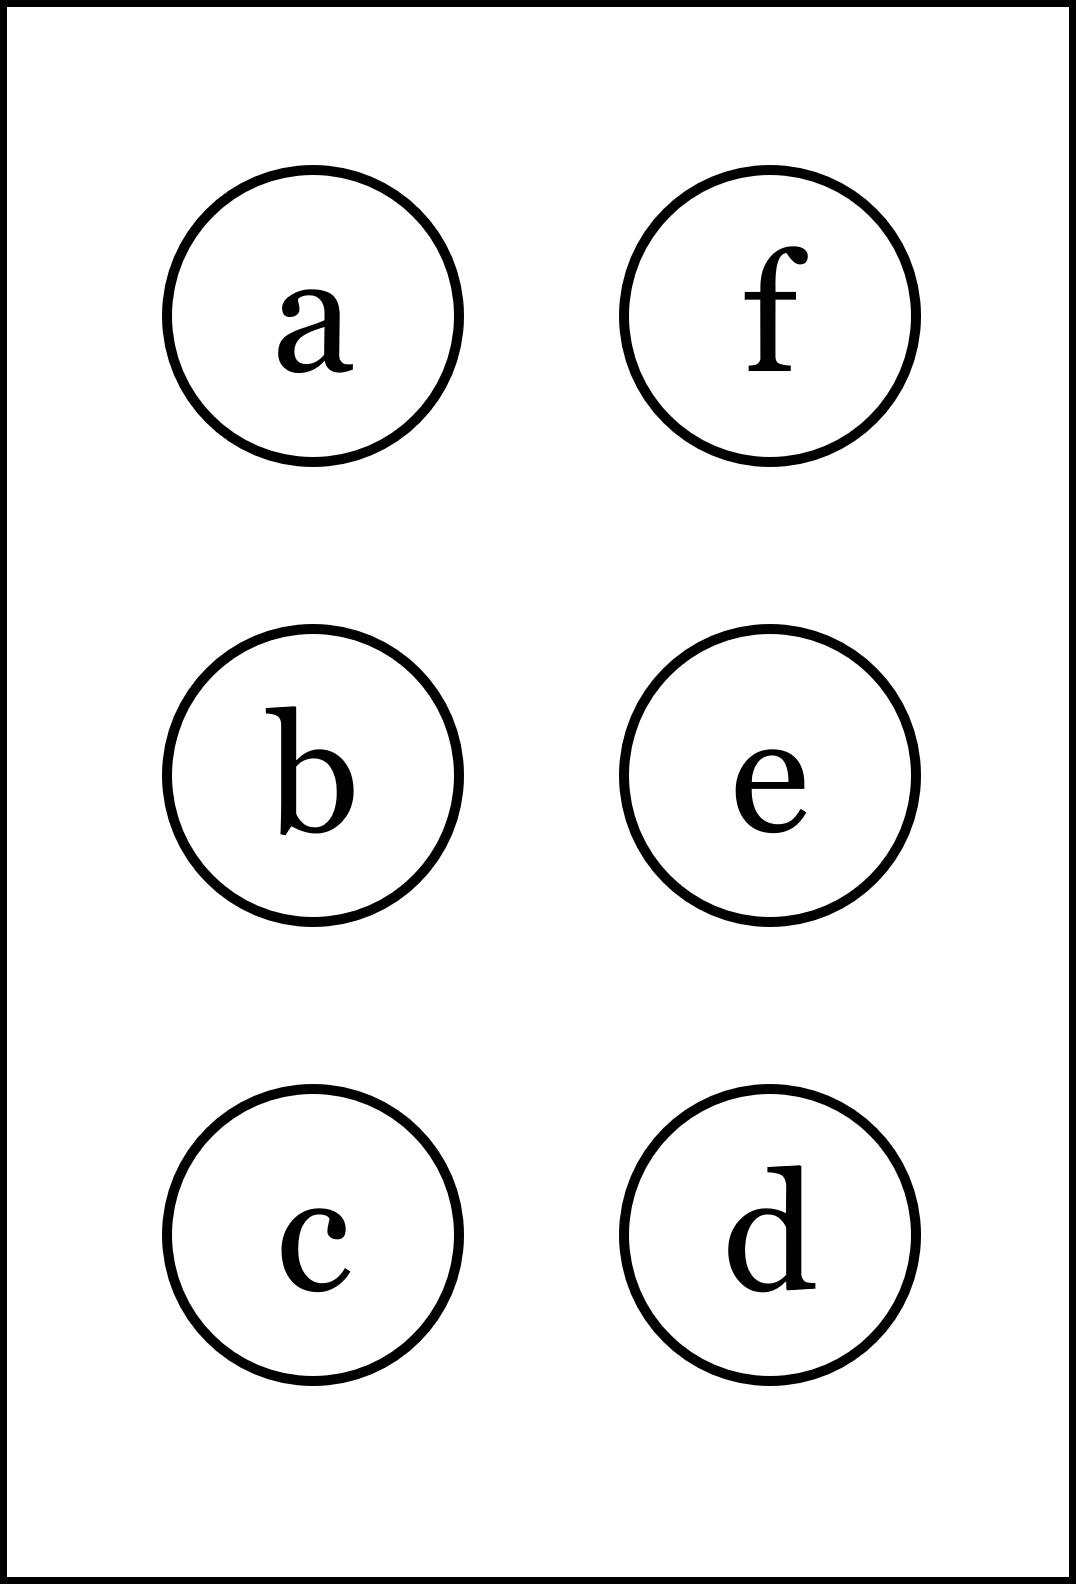
\includegraphics[height=40mm]{../images/braille.png}
{\small Písmeno Braillovej abecedy}
\end{center}
\end{minipage}
\end{center}
\end{minipage}
&
\begin{minipage}[c][104.5mm][t]{0.5\linewidth}
\begin{center}
\vspace{7mm}
{\huge Limity, skupina \textit{Alpha $\alpha$} -\romannumeral2}\\[5mm]
\textit{Meno:}\phantom{xxxxxxxxxxxxxxxxxxxxxxxxxxxxxxxxxxxxxxxxxxxxxxxxxxxxxxxxxxxxxxxxx}\\[5mm]
\begin{minipage}{0.95\linewidth}
\begin{center}
\textbf{Vypočti limity}. Pokud se výsledky shodujú s tými za otazníky, tak napravo\\obarvi příslušející kroužek načerno. \textbf{Spolu odevzdejte výsledné slovo}.
\end{center}
\end{minipage}
\\[1mm]
\begin{minipage}{0.79\linewidth}
\begin{center}
\begin{varwidth}{\linewidth}
\begin{enumerate}
\normalsize
\item $\lim\limits_{n\to\infty}\cfrac{-6+5n}{-2-9n}$\quad \dotfill\; ???\;\dotfill \quad $\nicefrac{-5}{9}$
\item $\lim\limits_{n\to\infty}\cfrac{6(-2+3n)}{(-5n-4)^2}$\quad \dotfill\; ???\;\dotfill \quad $\nicefrac{-3}{5}$
\item $\lim\limits_{n\to\infty}\cfrac{(4+3n)^2}{n^2+2n-2}$\quad \dotfill\; ???\;\dotfill \quad $\nicefrac{3}{2}$
\item $\lim\limits_{n\to\infty}\cfrac{2^{n-2}}{2^{n-2}}$\quad \dotfill\; ???\;\dotfill \quad $1$
\item $\lim\limits_{n\to\infty}\cfrac{\left(\frac{2}{3}\right)^n -2}{3n^{16}}$\quad \dotfill\; ???\;\dotfill \quad $-\infty$
\item $\lim\limits_{n\to\infty}\cfrac{-4\cdot 2^{n-2}-6\cdot 3^{n-2}}{-3\cdot 3^{n-2}-6\cdot 2^{n-1}}$\quad \dotfill\; ???\;\dotfill \quad $1$
\end{enumerate}
\end{varwidth}
\end{center}
\end{minipage}
\begin{minipage}{0.20\linewidth}
\begin{center}
{\Huge\bfseries 2.} \\[2mm]
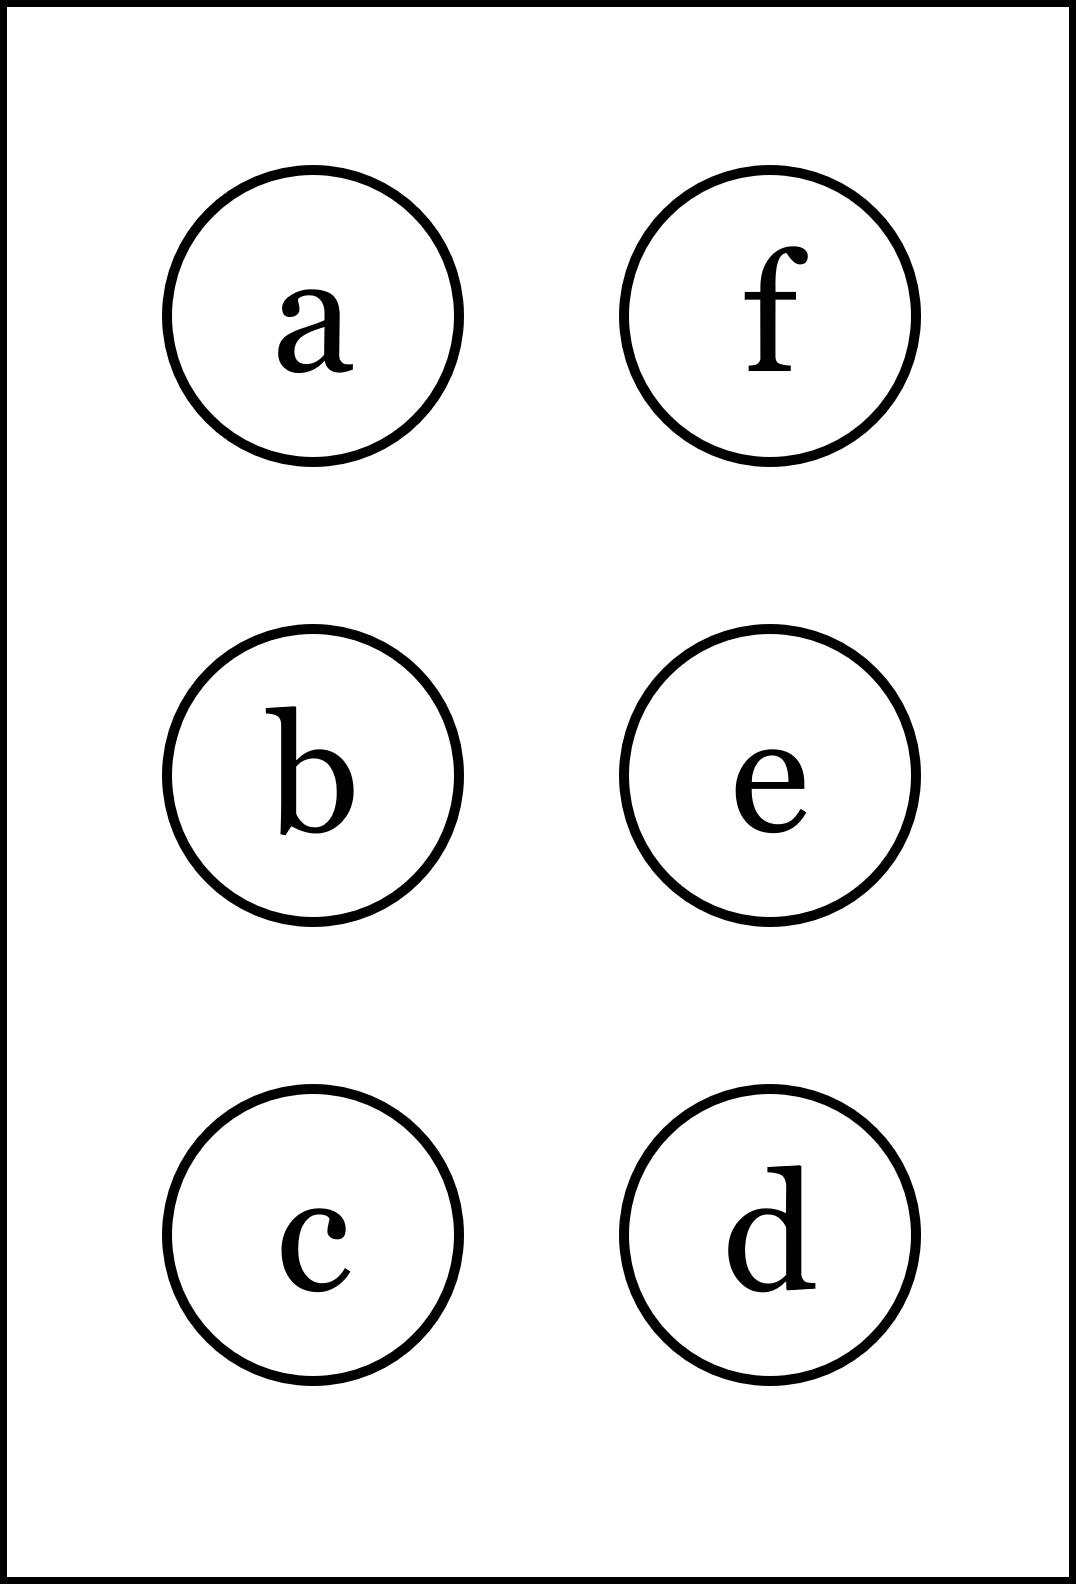
\includegraphics[height=40mm]{../images/braille.png}
{\small Písmeno Braillovej abecedy}
\end{center}
\end{minipage}
\end{center}
\end{minipage}
\\ \hdashline
\begin{minipage}[c][104.5mm][t]{0.5\linewidth}
\begin{center}
\vspace{7mm}
{\huge Limity, skupina \textit{Alpha $\alpha$} -\romannumeral3}\\[5mm]
\textit{Meno:}\phantom{xxxxxxxxxxxxxxxxxxxxxxxxxxxxxxxxxxxxxxxxxxxxxxxxxxxxxxxxxxxxxxxxx}\\[5mm]
\begin{minipage}{0.95\linewidth}
\begin{center}
\textbf{Vypočti limity}. Pokud se výsledky shodujú s tými za otazníky, tak napravo\\obarvi příslušející kroužek načerno. \textbf{Spolu odevzdejte výsledné slovo}.
\end{center}
\end{minipage}
\\[1mm]
\begin{minipage}{0.79\linewidth}
\begin{center}
\begin{varwidth}{\linewidth}
\begin{enumerate}
\normalsize
\item $\lim\limits_{n\to\infty}\cfrac{-5+6n}{3+6n}$\quad \dotfill\; ???\;\dotfill \quad $1$
\item $\lim\limits_{n\to\infty}\cfrac{6(4-2n)}{(-5n+2)^2}$\quad \dotfill\; ???\;\dotfill \quad $0$
\item $\lim\limits_{n\to\infty}\cfrac{(-1+8n)^2}{n^2+2n-8}$\quad \dotfill\; ???\;\dotfill \quad $64$
\item $\lim\limits_{n\to\infty}\cfrac{2^{n-1}}{2^{n+3}}$\quad \dotfill\; ???\;\dotfill \quad $0.5$
\item $\lim\limits_{n\to\infty}\cfrac{\left(\frac{3}{4}\right)^n +4}{-3n^{-6}}$\quad \dotfill\; ???\;\dotfill \quad $\infty$
\item $\lim\limits_{n\to\infty}\cfrac{12\cdot 3^{n+1}+16\cdot 4^{n-1}}{-9\cdot 4^{n-1}+9\cdot 3^{n-2}}$\quad \dotfill\; ???\;\dotfill \quad $\nicefrac{-16}{27}$
\end{enumerate}
\end{varwidth}
\end{center}
\end{minipage}
\begin{minipage}{0.20\linewidth}
\begin{center}
{\Huge\bfseries 3.} \\[2mm]
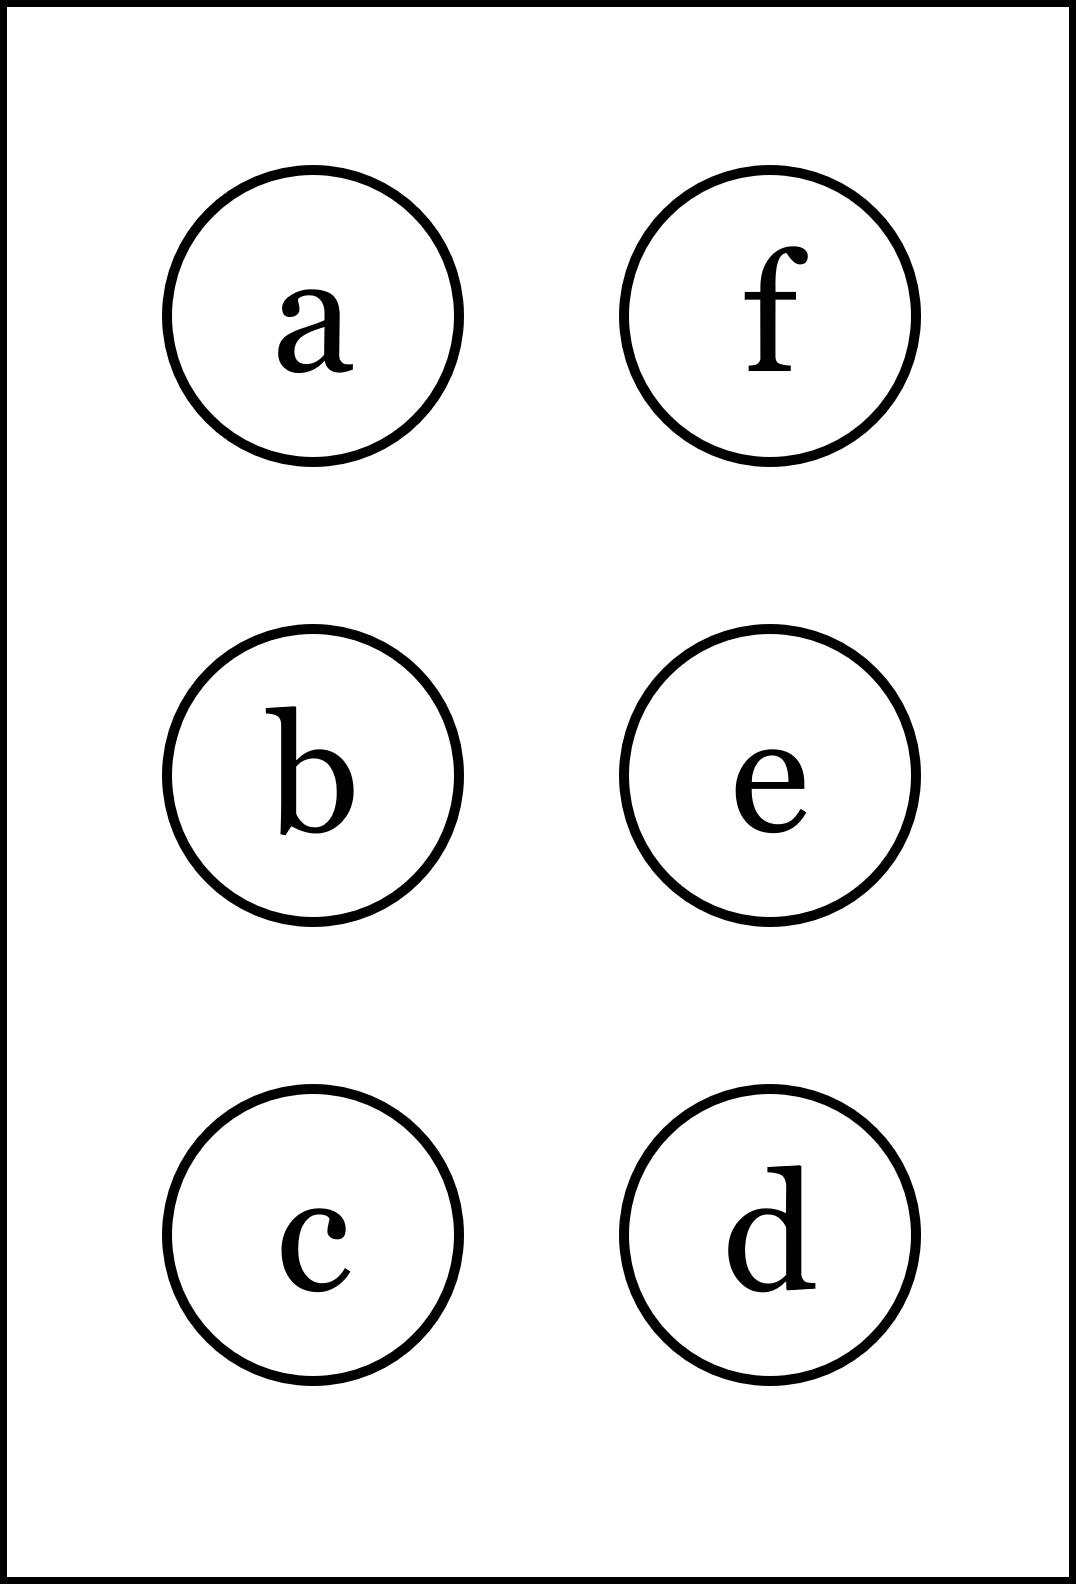
\includegraphics[height=40mm]{../images/braille.png}
{\small Písmeno Braillovej abecedy}
\end{center}
\end{minipage}
\end{center}
\end{minipage}
&
\begin{minipage}[c][104.5mm][t]{0.5\linewidth}
\begin{center}
\vspace{7mm}
{\huge Limity, skupina \textit{Alpha $\alpha$} -\romannumeral4}\\[5mm]
\textit{Meno:}\phantom{xxxxxxxxxxxxxxxxxxxxxxxxxxxxxxxxxxxxxxxxxxxxxxxxxxxxxxxxxxxxxxxxx}\\[5mm]
\begin{minipage}{0.95\linewidth}
\begin{center}
\textbf{Vypočti limity}. Pokud se výsledky shodujú s tými za otazníky, tak napravo\\obarvi příslušející kroužek načerno. \textbf{Spolu odevzdejte výsledné slovo}.
\end{center}
\end{minipage}
\\[1mm]
\begin{minipage}{0.79\linewidth}
\begin{center}
\begin{varwidth}{\linewidth}
\begin{enumerate}
\normalsize
\item $\lim\limits_{n\to\infty}\cfrac{-4+2n}{-6+5n}$\quad \dotfill\; ???\;\dotfill \quad $\nicefrac{2}{5}$
\item $\lim\limits_{n\to\infty}\cfrac{-6(-4+3n)}{(-9n-3)^2}$\quad \dotfill\; ???\;\dotfill \quad $\infty$
\item $\lim\limits_{n\to\infty}\cfrac{(2+4n)^2}{n^2-4n-4}$\quad \dotfill\; ???\;\dotfill \quad $\infty$
\item $\lim\limits_{n\to\infty}\cfrac{2^{n+2}}{2^{n-1}}$\quad \dotfill\; ???\;\dotfill \quad $\nicefrac{1}{8}$
\item $\lim\limits_{n\to\infty}\cfrac{\left(\frac{1}{4}\right)^n +1}{n^{-12}}$\quad \dotfill\; ???\;\dotfill \quad $0$
\item $\lim\limits_{n\to\infty}\cfrac{9\cdot 2^{n-2}+3\cdot 3^{n+1}}{-2\cdot 3^{n-1}-4\cdot 2^{n-1}}$\quad \dotfill\; ???\;\dotfill \quad $\nicefrac{-1}{2}$
\end{enumerate}
\end{varwidth}
\end{center}
\end{minipage}
\begin{minipage}{0.20\linewidth}
\begin{center}
{\Huge\bfseries 4.} \\[2mm]
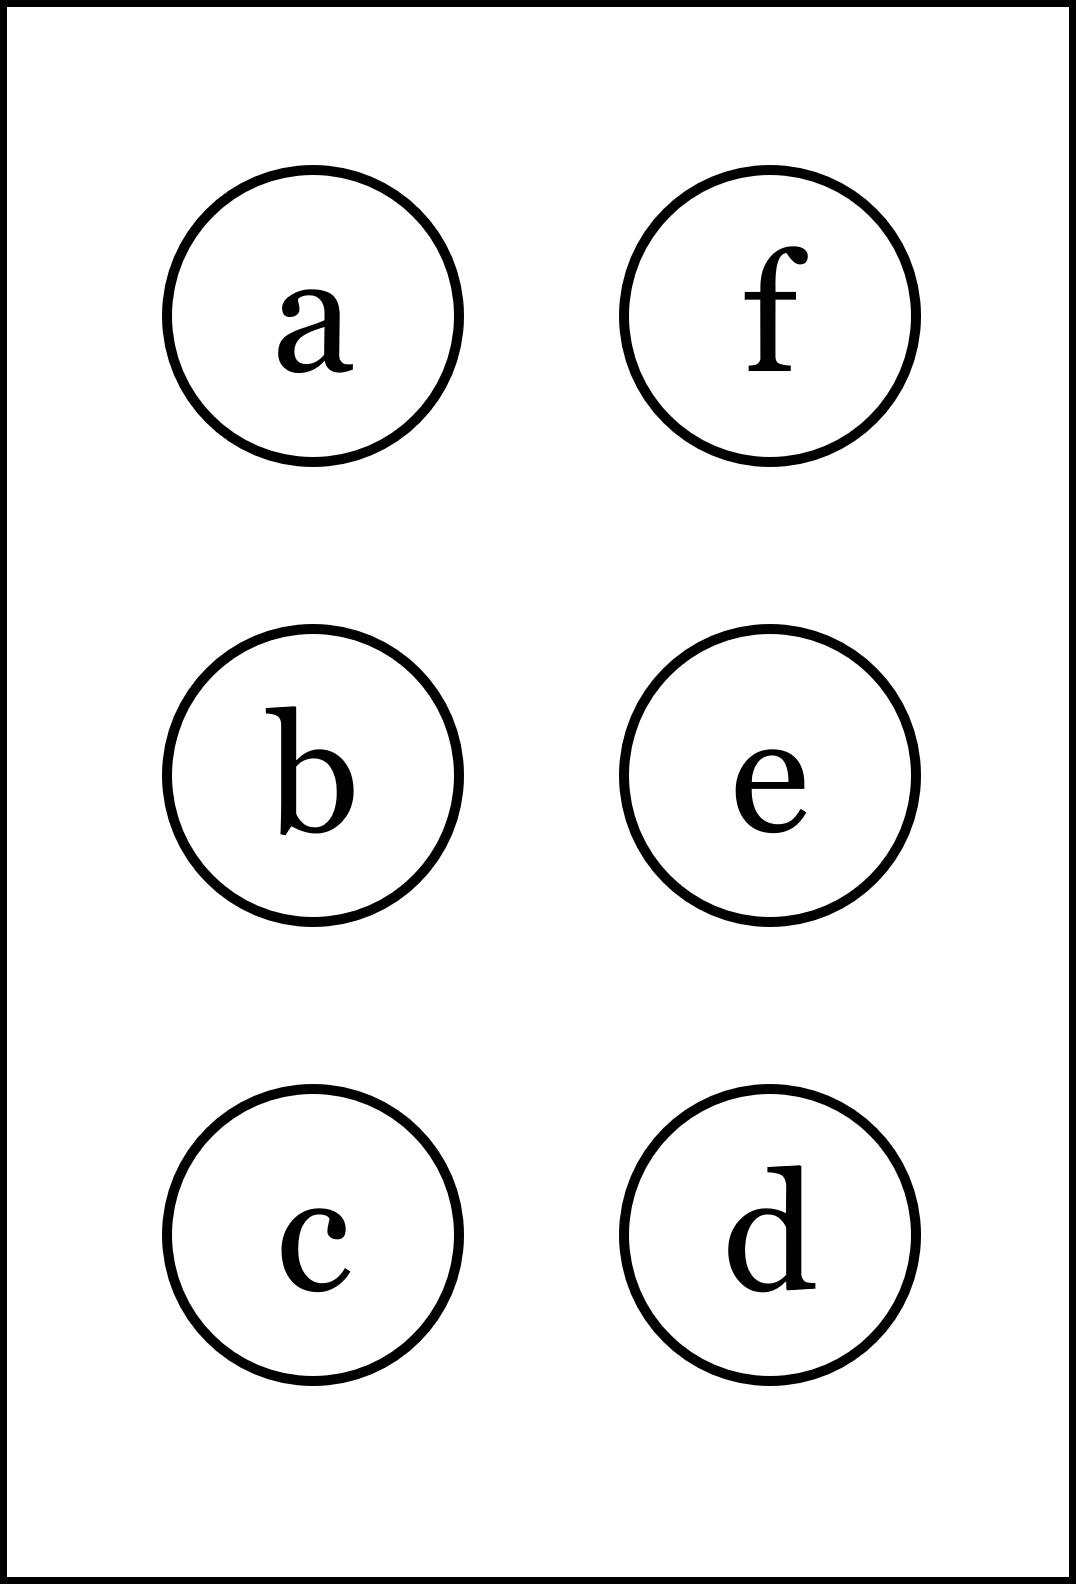
\includegraphics[height=40mm]{../images/braille.png}
{\small Písmeno Braillovej abecedy}
\end{center}
\end{minipage}
\end{center}
\end{minipage}
%
\end{tabular}
\newpage
\thispagestyle{empty}
\begin{tabular}{c:c}
\begin{minipage}[c][104.5mm][t]{0.5\linewidth}
\begin{center}
\vspace{7mm}
{\huge Limity, skupina \textit{Beta $\beta$} -\romannumeral1}\\[5mm]
\textit{Meno:}\phantom{xxxxxxxxxxxxxxxxxxxxxxxxxxxxxxxxxxxxxxxxxxxxxxxxxxxxxxxxxxxxxxxxx}\\[5mm]
\begin{minipage}{0.95\linewidth}
\begin{center}
\textbf{Vypočti limity}. Pokud se výsledky shodujú s tými za otazníky, tak napravo\\obarvi příslušející kroužek načerno. \textbf{Spolu odevzdejte výsledné slovo}.
\end{center}
\end{minipage}
\\[1mm]
\begin{minipage}{0.79\linewidth}
\begin{center}
\begin{varwidth}{\linewidth}
\begin{enumerate}
\normalsize
\item $\lim\limits_{n\to\infty}\cfrac{-5+2n}{-8-n}$\quad \dotfill\; ???\;\dotfill \quad $0$
\item $\lim\limits_{n\to\infty}\cfrac{-5(2-2n)}{(-n+3)^2}$\quad \dotfill\; ???\;\dotfill \quad $0$
\item $\lim\limits_{n\to\infty}\cfrac{(-9+6n)^2}{n^2-4n+9}$\quad \dotfill\; ???\;\dotfill \quad $36$
\item $\lim\limits_{n\to\infty}\cfrac{2^{n-2}}{2^{n-3}}$\quad \dotfill\; ???\;\dotfill \quad $\nicefrac{1}{2}$
\item $\lim\limits_{n\to\infty}\cfrac{\left(\frac{1}{3}\right)^n +3}{-n^{-8}}$\quad \dotfill\; ???\;\dotfill \quad $-\infty$
\item $\lim\limits_{n\to\infty}\cfrac{-2\cdot 2^{n-2}-2\cdot 3^{n+2}}{-6\cdot 3^{n+2}-9\cdot 2^{n-1}}$\quad \dotfill\; ???\;\dotfill \quad $\nicefrac{1}{3}$
\end{enumerate}
\end{varwidth}
\end{center}
\end{minipage}
\begin{minipage}{0.20\linewidth}
\begin{center}
{\Huge\bfseries 1.} \\[2mm]
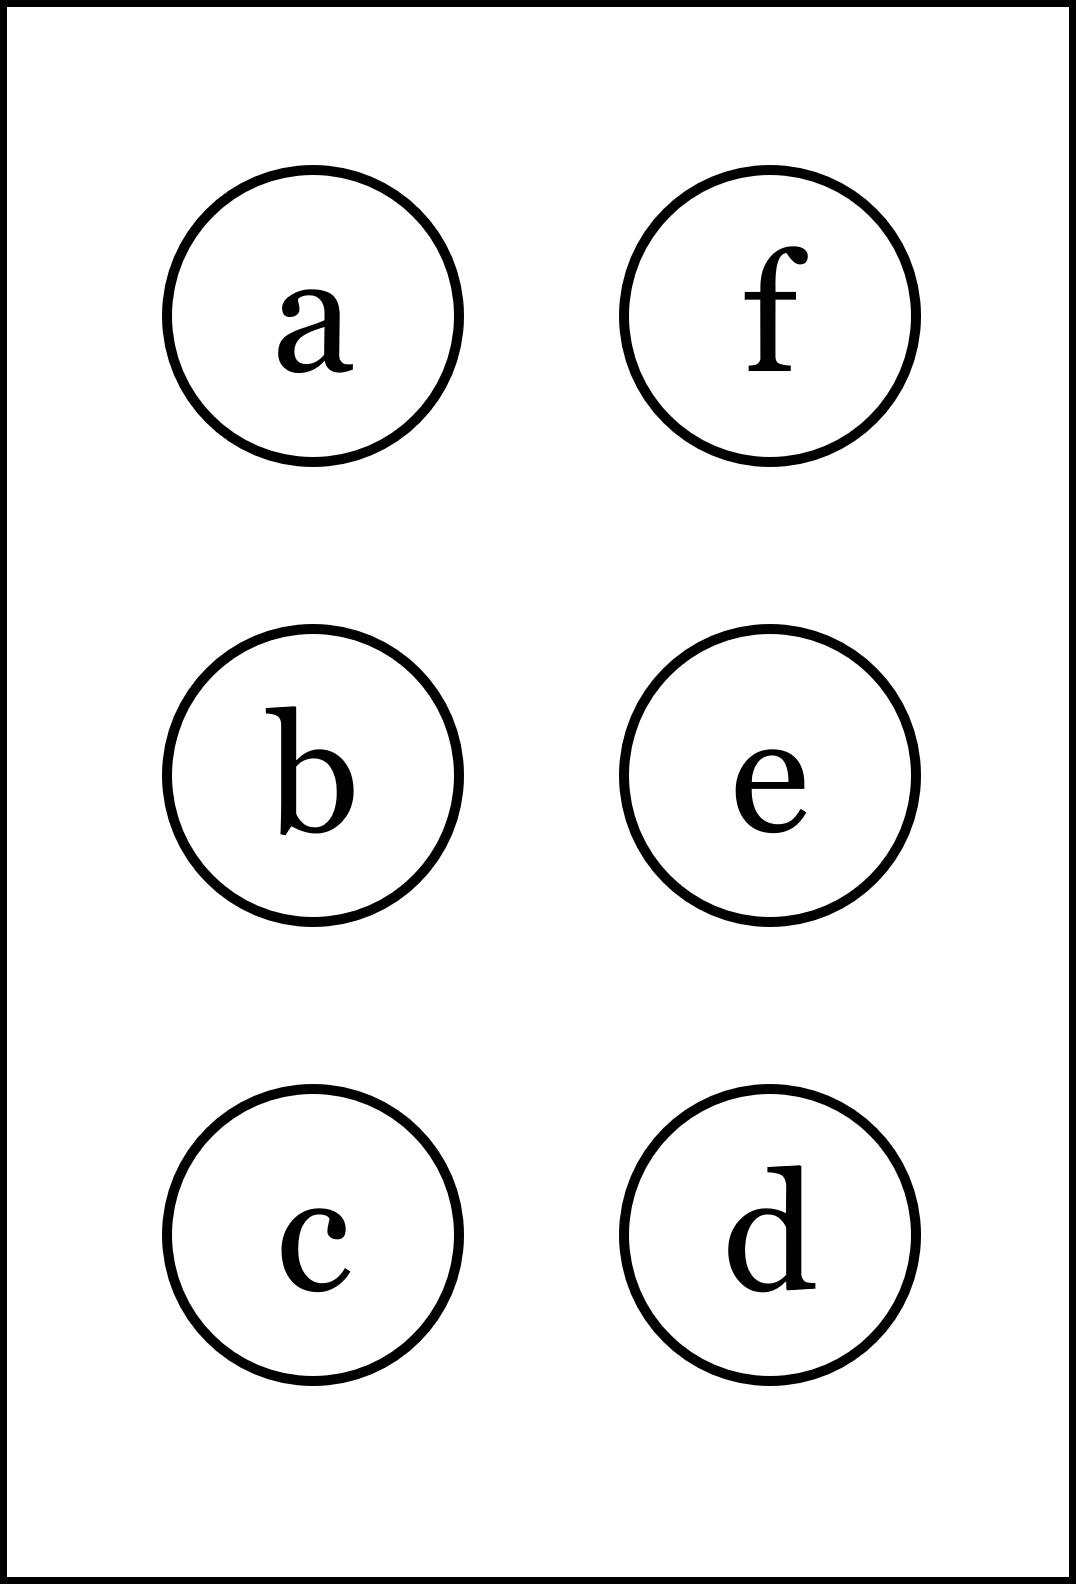
\includegraphics[height=40mm]{../images/braille.png}
{\small Písmeno Braillovej abecedy}
\end{center}
\end{minipage}
\end{center}
\end{minipage}
&
\begin{minipage}[c][104.5mm][t]{0.5\linewidth}
\begin{center}
\vspace{7mm}
{\huge Limity, skupina \textit{Beta $\beta$} -\romannumeral2}\\[5mm]
\textit{Meno:}\phantom{xxxxxxxxxxxxxxxxxxxxxxxxxxxxxxxxxxxxxxxxxxxxxxxxxxxxxxxxxxxxxxxxx}\\[5mm]
\begin{minipage}{0.95\linewidth}
\begin{center}
\textbf{Vypočti limity}. Pokud se výsledky shodujú s tými za otazníky, tak napravo\\obarvi příslušející kroužek načerno. \textbf{Spolu odevzdejte výsledné slovo}.
\end{center}
\end{minipage}
\\[1mm]
\begin{minipage}{0.79\linewidth}
\begin{center}
\begin{varwidth}{\linewidth}
\begin{enumerate}
\normalsize
\item $\lim\limits_{n\to\infty}\cfrac{-1-7n}{4-n}$\quad \dotfill\; ???\;\dotfill \quad $7$
\item $\lim\limits_{n\to\infty}\cfrac{-9(1-5n)}{(4n-1)^2}$\quad \dotfill\; ???\;\dotfill \quad $0$
\item $\lim\limits_{n\to\infty}\cfrac{(-6+3n)^2}{n^2+n-2}$\quad \dotfill\; ???\;\dotfill \quad $9$
\item $\lim\limits_{n\to\infty}\cfrac{3^{n-3}}{3^{n+1}}$\quad \dotfill\; ???\;\dotfill \quad $0$
\item $\lim\limits_{n\to\infty}\cfrac{\left(\frac{4}{2}\right)^n +3}{-3n^{16}}$\quad \dotfill\; ???\;\dotfill \quad $\infty$
\item $\lim\limits_{n\to\infty}\cfrac{3\cdot 2^{n+1}-3\cdot 3^{n+1}}{4\cdot 3^{n+2}+4\cdot 2^{n+2}}$\quad \dotfill\; ???\;\dotfill \quad $\nicefrac{-9}{4}$
\end{enumerate}
\end{varwidth}
\end{center}
\end{minipage}
\begin{minipage}{0.20\linewidth}
\begin{center}
{\Huge\bfseries 2.} \\[2mm]
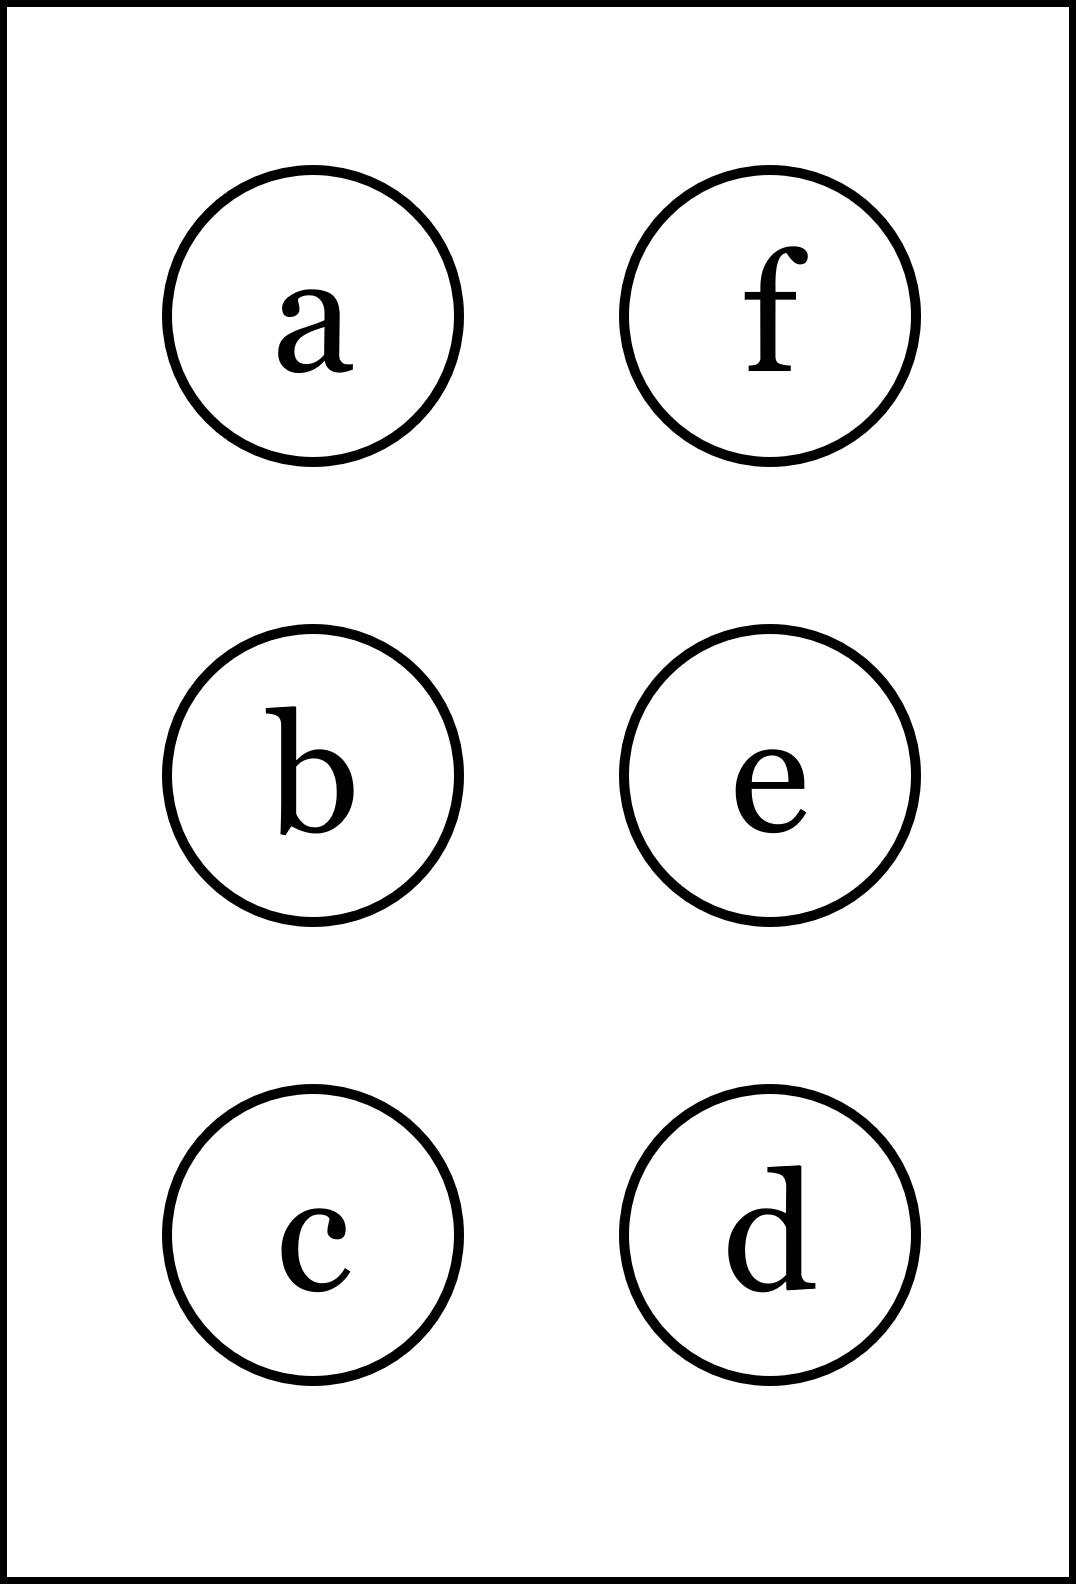
\includegraphics[height=40mm]{../images/braille.png}
{\small Písmeno Braillovej abecedy}
\end{center}
\end{minipage}
\end{center}
\end{minipage}
\\ \hdashline
\begin{minipage}[c][104.5mm][t]{0.5\linewidth}
\begin{center}
\vspace{7mm}
{\huge Limity, skupina \textit{Beta $\beta$} -\romannumeral3}\\[5mm]
\textit{Meno:}\phantom{xxxxxxxxxxxxxxxxxxxxxxxxxxxxxxxxxxxxxxxxxxxxxxxxxxxxxxxxxxxxxxxxx}\\[5mm]
\begin{minipage}{0.95\linewidth}
\begin{center}
\textbf{Vypočti limity}. Pokud se výsledky shodujú s tými za otazníky, tak napravo\\obarvi příslušející kroužek načerno. \textbf{Spolu odevzdejte výsledné slovo}.
\end{center}
\end{minipage}
\\[1mm]
\begin{minipage}{0.79\linewidth}
\begin{center}
\begin{varwidth}{\linewidth}
\begin{enumerate}
\normalsize
\item $\lim\limits_{n\to\infty}\cfrac{6-6n}{-3+6n}$\quad \dotfill\; ???\;\dotfill \quad $-1$
\item $\lim\limits_{n\to\infty}\cfrac{-8(-4-2n)}{(n-1)^2}$\quad \dotfill\; ???\;\dotfill \quad $\infty$
\item $\lim\limits_{n\to\infty}\cfrac{(5-8n)^2}{n^2-2n-3}$\quad \dotfill\; ???\;\dotfill \quad $0$
\item $\lim\limits_{n\to\infty}\cfrac{3^{n+1}}{3^{n-3}}$\quad \dotfill\; ???\;\dotfill \quad $\infty$
\item $\lim\limits_{n\to\infty}\cfrac{\left(\frac{2}{4}\right)^n -2}{-4n^{-6}}$\quad \dotfill\; ???\;\dotfill \quad $-\infty$
\item $\lim\limits_{n\to\infty}\cfrac{-6\cdot 2^{n+1}+3\cdot 3^{n+1}}{2\cdot 3^{n-1}+6\cdot 2^{n+1}}$\quad \dotfill\; ???\;\dotfill \quad $\nicefrac{1}{2}$
\end{enumerate}
\end{varwidth}
\end{center}
\end{minipage}
\begin{minipage}{0.20\linewidth}
\begin{center}
{\Huge\bfseries 3.} \\[2mm]
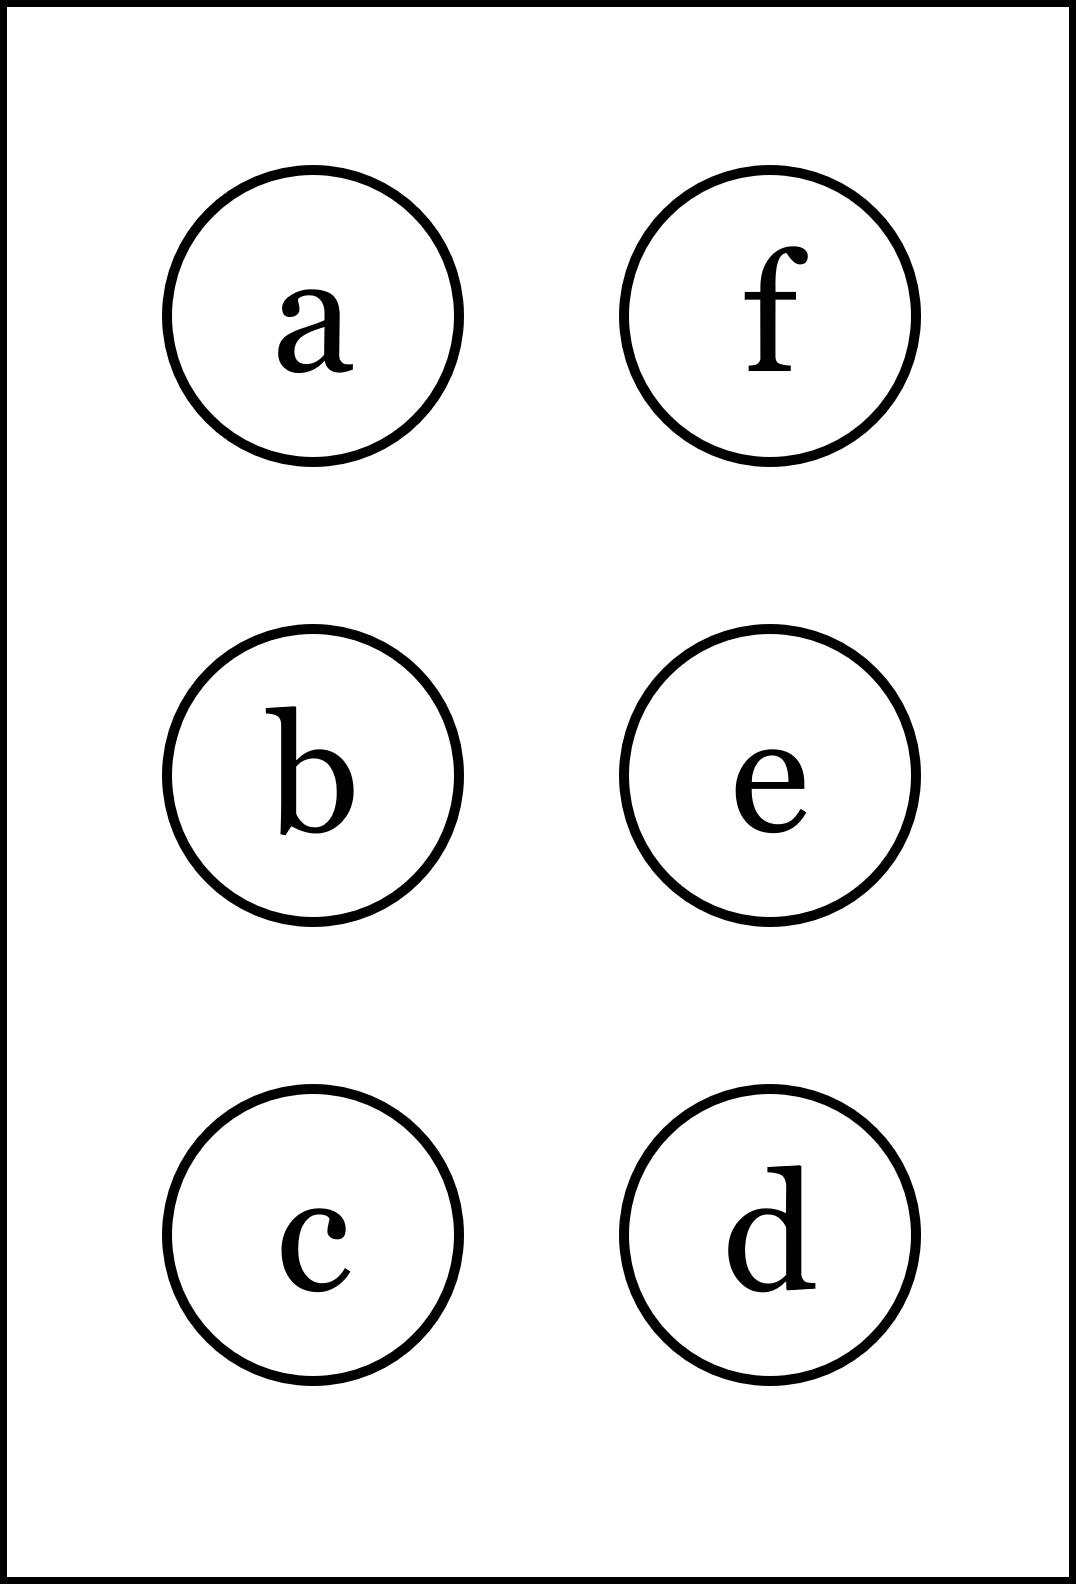
\includegraphics[height=40mm]{../images/braille.png}
{\small Písmeno Braillovej abecedy}
\end{center}
\end{minipage}
\end{center}
\end{minipage}
&
\begin{minipage}[c][104.5mm][t]{0.5\linewidth}
\begin{center}
\vspace{7mm}
{\huge Limity, skupina \textit{Beta $\beta$} -\romannumeral4}\\[5mm]
\textit{Meno:}\phantom{xxxxxxxxxxxxxxxxxxxxxxxxxxxxxxxxxxxxxxxxxxxxxxxxxxxxxxxxxxxxxxxxx}\\[5mm]
\begin{minipage}{0.95\linewidth}
\begin{center}
\textbf{Vypočti limity}. Pokud se výsledky shodujú s tými za otazníky, tak napravo\\obarvi příslušející kroužek načerno. \textbf{Spolu odevzdejte výsledné slovo}.
\end{center}
\end{minipage}
\\[1mm]
\begin{minipage}{0.79\linewidth}
\begin{center}
\begin{varwidth}{\linewidth}
\begin{enumerate}
\normalsize
\item $\lim\limits_{n\to\infty}\cfrac{-1-2n}{-5+3n}$\quad \dotfill\; ???\;\dotfill \quad $\nicefrac{-2}{3}$
\item $\lim\limits_{n\to\infty}\cfrac{-4(-2+2n)}{(-4n+1)^2}$\quad \dotfill\; ???\;\dotfill \quad $\infty$
\item $\lim\limits_{n\to\infty}\cfrac{(-2+4n)^2}{n^2+n+4}$\quad \dotfill\; ???\;\dotfill \quad $16$
\item $\lim\limits_{n\to\infty}\cfrac{3^{n+2}}{3^{n+2}}$\quad \dotfill\; ???\;\dotfill \quad $9$
\item $\lim\limits_{n\to\infty}\cfrac{\left(\frac{2}{4}\right)^n -3}{-n^{-12}}$\quad \dotfill\; ???\;\dotfill \quad $3$
\item $\lim\limits_{n\to\infty}\cfrac{3\cdot 2^{n-1}-9\cdot 3^{n-1}}{2\cdot 3^{n+1}+6\cdot 2^{n+1}}$\quad \dotfill\; ???\;\dotfill \quad $\nicefrac{-27}{2}$
\end{enumerate}
\end{varwidth}
\end{center}
\end{minipage}
\begin{minipage}{0.20\linewidth}
\begin{center}
{\Huge\bfseries 4.} \\[2mm]
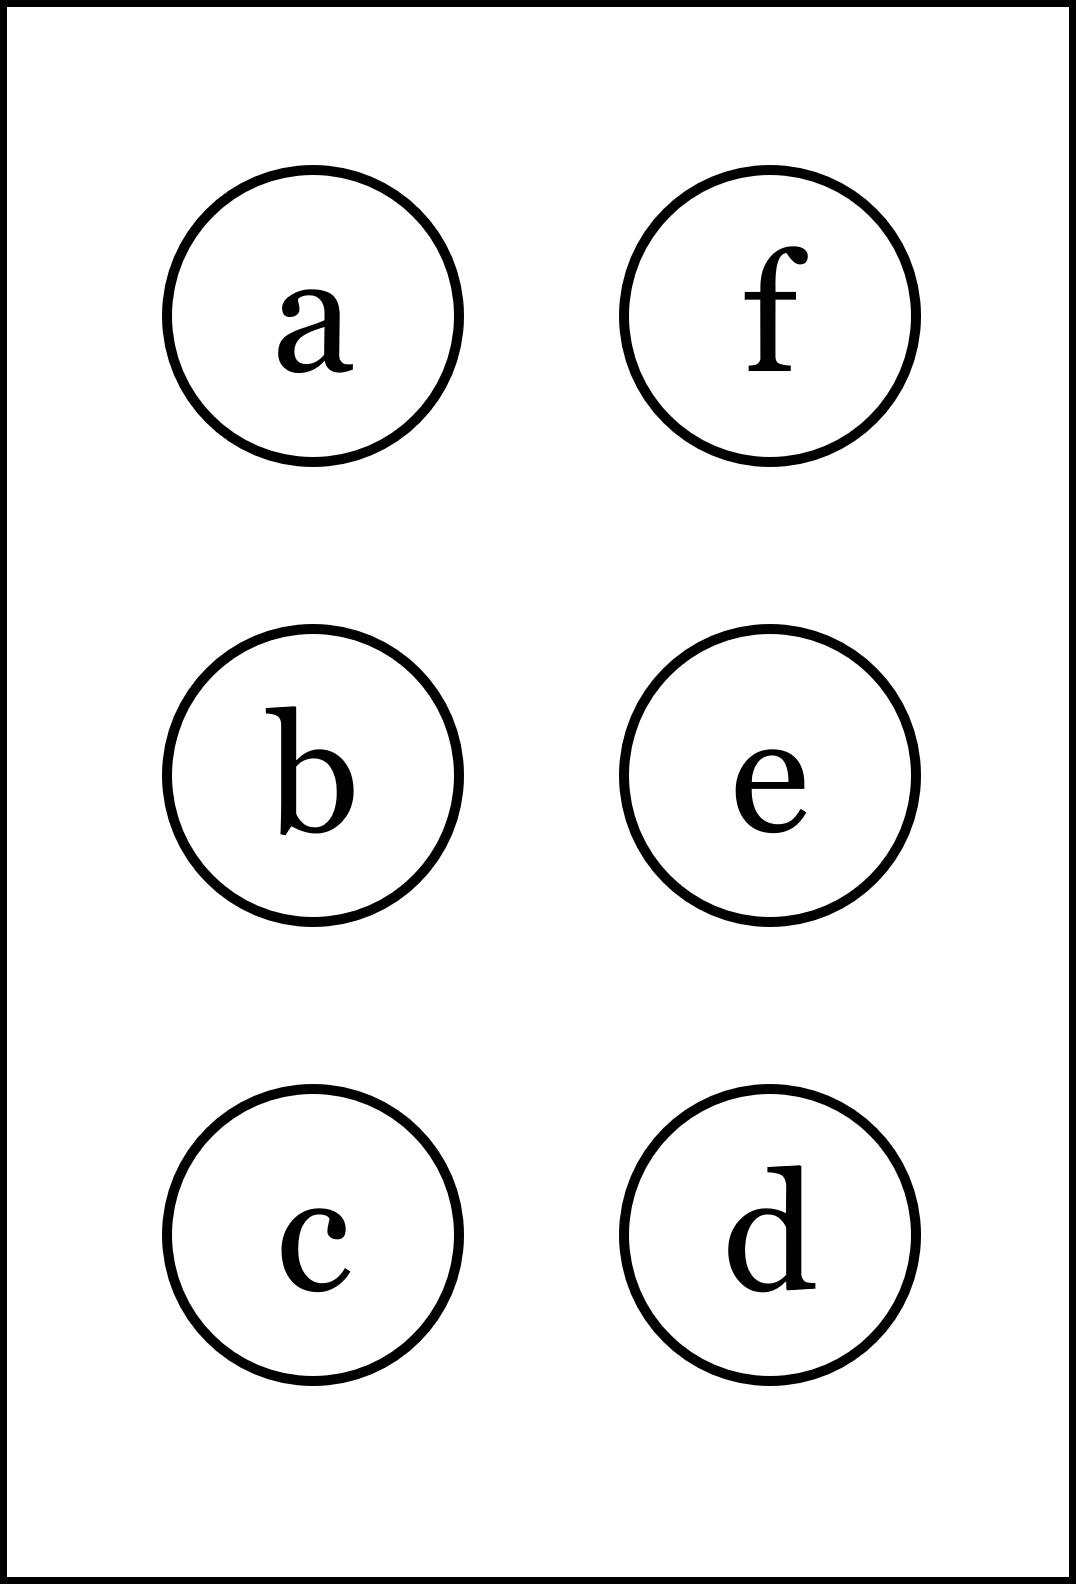
\includegraphics[height=40mm]{../images/braille.png}
{\small Písmeno Braillovej abecedy}
\end{center}
\end{minipage}
\end{center}
\end{minipage}
%
\end{tabular}
\newpage
\thispagestyle{empty}
\begin{tabular}{c:c}
\begin{minipage}[c][104.5mm][t]{0.5\linewidth}
\begin{center}
\vspace{7mm}
{\huge Limity, skupina \textit{Gamma $\gamma$} -\romannumeral1}\\[5mm]
\textit{Meno:}\phantom{xxxxxxxxxxxxxxxxxxxxxxxxxxxxxxxxxxxxxxxxxxxxxxxxxxxxxxxxxxxxxxxxx}\\[5mm]
\begin{minipage}{0.95\linewidth}
\begin{center}
\textbf{Vypočti limity}. Pokud se výsledky shodujú s tými za otazníky, tak napravo\\obarvi příslušející kroužek načerno. \textbf{Spolu odevzdejte výsledné slovo}.
\end{center}
\end{minipage}
\\[1mm]
\begin{minipage}{0.79\linewidth}
\begin{center}
\begin{varwidth}{\linewidth}
\begin{enumerate}
\normalsize
\item $\lim\limits_{n\to\infty}\cfrac{2+6n}{4+8n}$\quad \dotfill\; ???\;\dotfill \quad $\infty$
\item $\lim\limits_{n\to\infty}\cfrac{-5(4-6n)}{(9n-3)^2}$\quad \dotfill\; ???\;\dotfill \quad -5
\item $\lim\limits_{n\to\infty}\cfrac{(-5+4n)^2}{n^2+9n-3}$\quad \dotfill\; ???\;\dotfill \quad $16$
\item $\lim\limits_{n\to\infty}\cfrac{4^{n-2}}{4^{n-1}}$\quad \dotfill\; ???\;\dotfill \quad $\nicefrac{1}{4}$
\item $\lim\limits_{n\to\infty}\cfrac{\left(\frac{1}{3}\right)^n -1}{n^{-12}}$\quad \dotfill\; ???\;\dotfill \quad $-12$
\item $\lim\limits_{n\to\infty}\cfrac{4\cdot 2^{n-2}-3\cdot 3^{n+1}}{6\cdot 3^{n+1}+4\cdot 2^{n+1}}$\quad \dotfill\; ???\;\dotfill \quad $\nicefrac{-1}{2}$
\end{enumerate}
\end{varwidth}
\end{center}
\end{minipage}
\begin{minipage}{0.20\linewidth}
\begin{center}
{\Huge\bfseries 1.} \\[2mm]
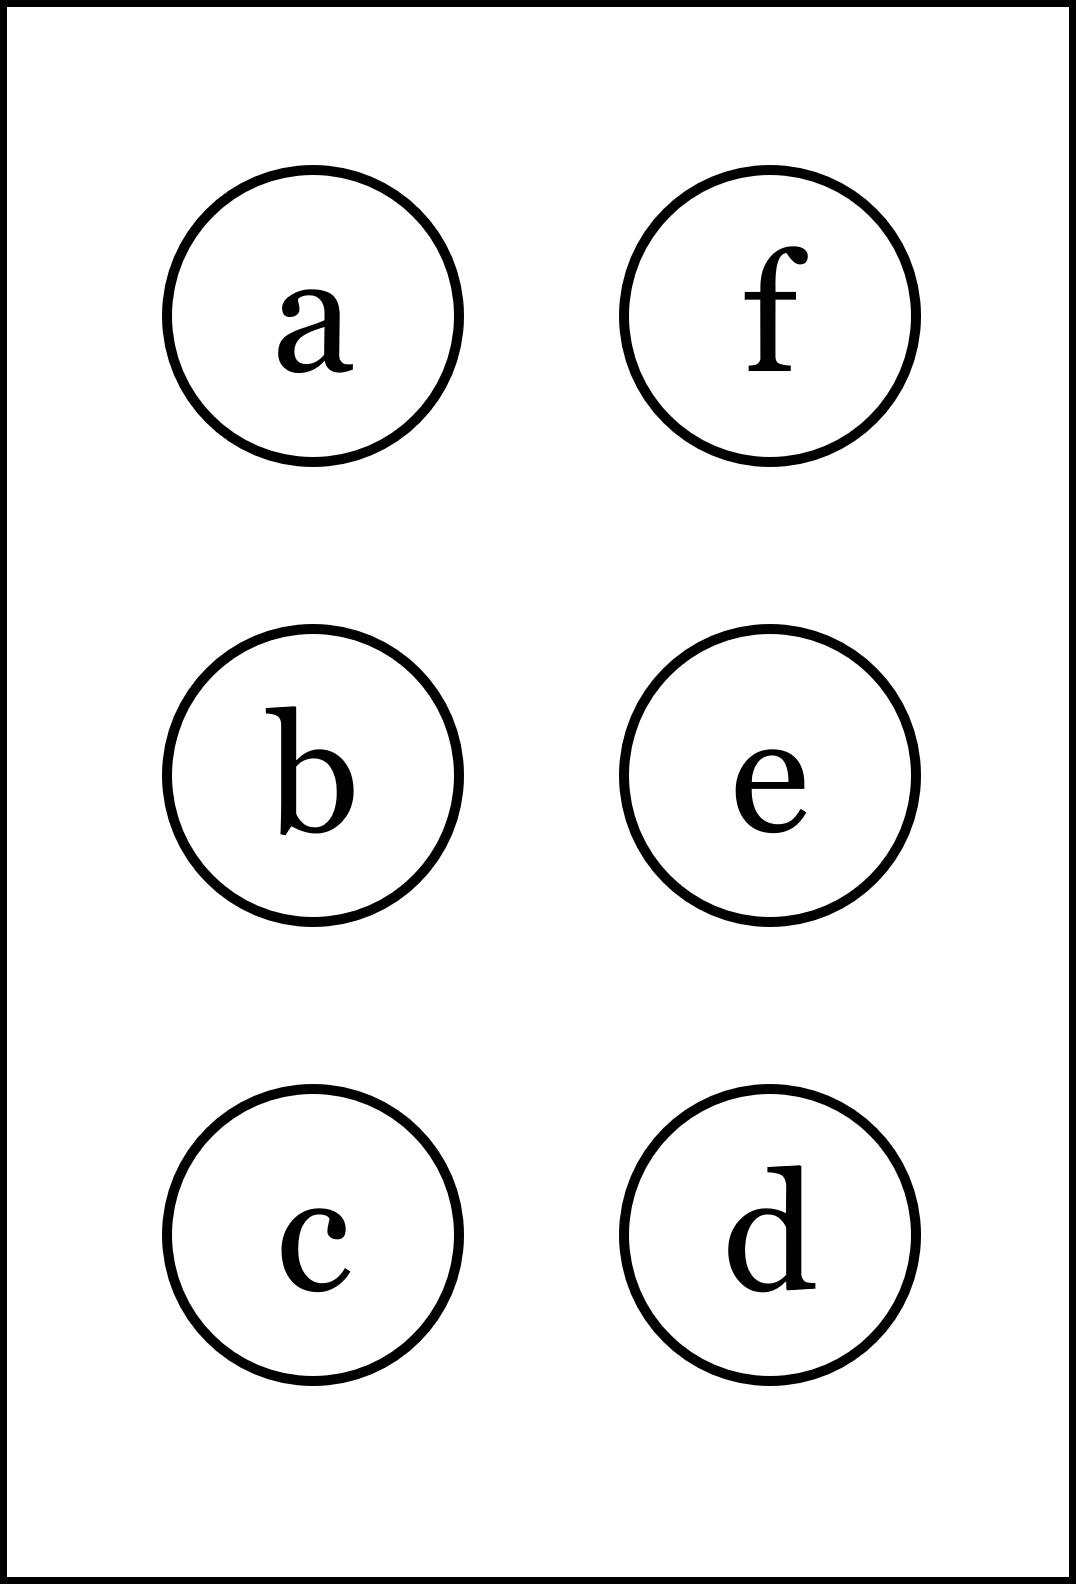
\includegraphics[height=40mm]{../images/braille.png}
{\small Písmeno Braillovej abecedy}
\end{center}
\end{minipage}
\end{center}
\end{minipage}
&
\begin{minipage}[c][104.5mm][t]{0.5\linewidth}
\begin{center}
\vspace{7mm}
{\huge Limity, skupina \textit{Gamma $\gamma$} -\romannumeral2}\\[5mm]
\textit{Meno:}\phantom{xxxxxxxxxxxxxxxxxxxxxxxxxxxxxxxxxxxxxxxxxxxxxxxxxxxxxxxxxxxxxxxxx}\\[5mm]
\begin{minipage}{0.95\linewidth}
\begin{center}
\textbf{Vypočti limity}. Pokud se výsledky shodujú s tými za otazníky, tak napravo\\obarvi příslušející kroužek načerno. \textbf{Spolu odevzdejte výsledné slovo}.
\end{center}
\end{minipage}
\\[1mm]
\begin{minipage}{0.79\linewidth}
\begin{center}
\begin{varwidth}{\linewidth}
\begin{enumerate}
\normalsize
\item $\lim\limits_{n\to\infty}\cfrac{5-5n}{1-2n}$\quad \dotfill\; ???\;\dotfill \quad $\infty$
\item $\lim\limits_{n\to\infty}\cfrac{-1(6-8n)}{(7n-3)^2}$\quad \dotfill\; ???\;\dotfill \quad $0$
\item $\lim\limits_{n\to\infty}\cfrac{(-7-4n)^2}{n^2-3n+1}$\quad \dotfill\; ???\;\dotfill \quad $16$
\item $\lim\limits_{n\to\infty}\cfrac{2^{n-1}}{2^{n+2}}$\quad \dotfill\; ???\;\dotfill \quad $\infty$
\item $\lim\limits_{n\to\infty}\cfrac{\left(\frac{2}{3}\right)^n -2}{-2n^{-6}}$\quad \dotfill\; ???\;\dotfill \quad $-\infty$
\item $\lim\limits_{n\to\infty}\cfrac{2\cdot 2^{n+2}+9\cdot 3^{n+1}}{-9\cdot 3^{n+2}+4\cdot 2^{n+2}}$\quad \dotfill\; ???\;\dotfill \quad $\nicefrac{-1}{3}$
\end{enumerate}
\end{varwidth}
\end{center}
\end{minipage}
\begin{minipage}{0.20\linewidth}
\begin{center}
{\Huge\bfseries 2.} \\[2mm]
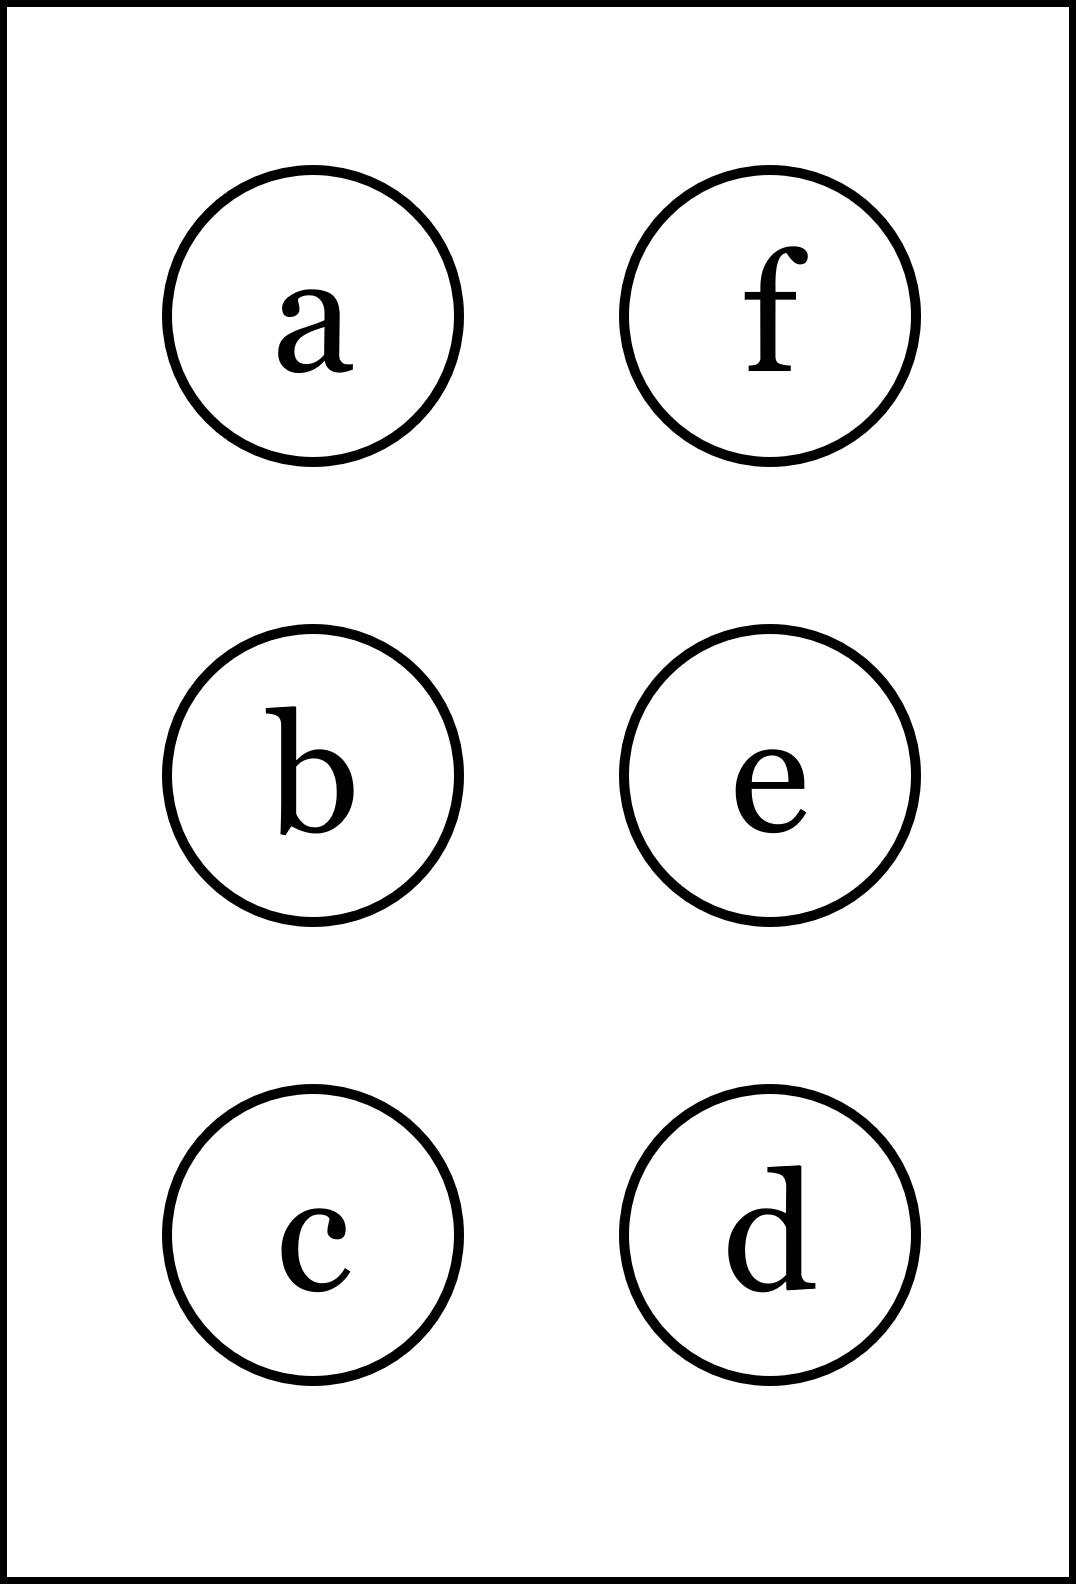
\includegraphics[height=40mm]{../images/braille.png}
{\small Písmeno Braillovej abecedy}
\end{center}
\end{minipage}
\end{center}
\end{minipage}
\\ \hdashline
\begin{minipage}[c][104.5mm][t]{0.5\linewidth}
\begin{center}
\vspace{7mm}
{\huge Limity, skupina \textit{Gamma $\gamma$} -\romannumeral3}\\[5mm]
\textit{Meno:}\phantom{xxxxxxxxxxxxxxxxxxxxxxxxxxxxxxxxxxxxxxxxxxxxxxxxxxxxxxxxxxxxxxxxx}\\[5mm]
\begin{minipage}{0.95\linewidth}
\begin{center}
\textbf{Vypočti limity}. Pokud se výsledky shodujú s tými za otazníky, tak napravo\\obarvi příslušející kroužek načerno. \textbf{Spolu odevzdejte výsledné slovo}.
\end{center}
\end{minipage}
\\[1mm]
\begin{minipage}{0.79\linewidth}
\begin{center}
\begin{varwidth}{\linewidth}
\begin{enumerate}
\normalsize
\item $\lim\limits_{n\to\infty}\cfrac{2+4n}{4+6n}$\quad \dotfill\; ???\;\dotfill \quad $0$
\item $\lim\limits_{n\to\infty}\cfrac{6(6-4n)}{(n-3)^2}$\quad \dotfill\; ???\;\dotfill \quad $0$
\item $\lim\limits_{n\to\infty}\cfrac{(2+2n)^2}{n^2+6n-3}$\quad \dotfill\; ???\;\dotfill \quad $4$
\item $\lim\limits_{n\to\infty}\cfrac{2^{n-2}}{2^{n-4}}$\quad \dotfill\; ???\;\dotfill \quad $0.25$
\item $\lim\limits_{n\to\infty}\cfrac{\left(\frac{1}{2}\right)^n -4}{-4n^{-16}}$\quad \dotfill\; ???\;\dotfill \quad $\infty$
\item $\lim\limits_{n\to\infty}\cfrac{-16\cdot 3^{n+1}+16\cdot 4^{n+1}}{-16\cdot 4^{n-2}+9\cdot 3^{n-2}}$\quad \dotfill\; ???\;\dotfill \quad $-64$
\end{enumerate}
\end{varwidth}
\end{center}
\end{minipage}
\begin{minipage}{0.20\linewidth}
\begin{center}
{\Huge\bfseries 3.} \\[2mm]
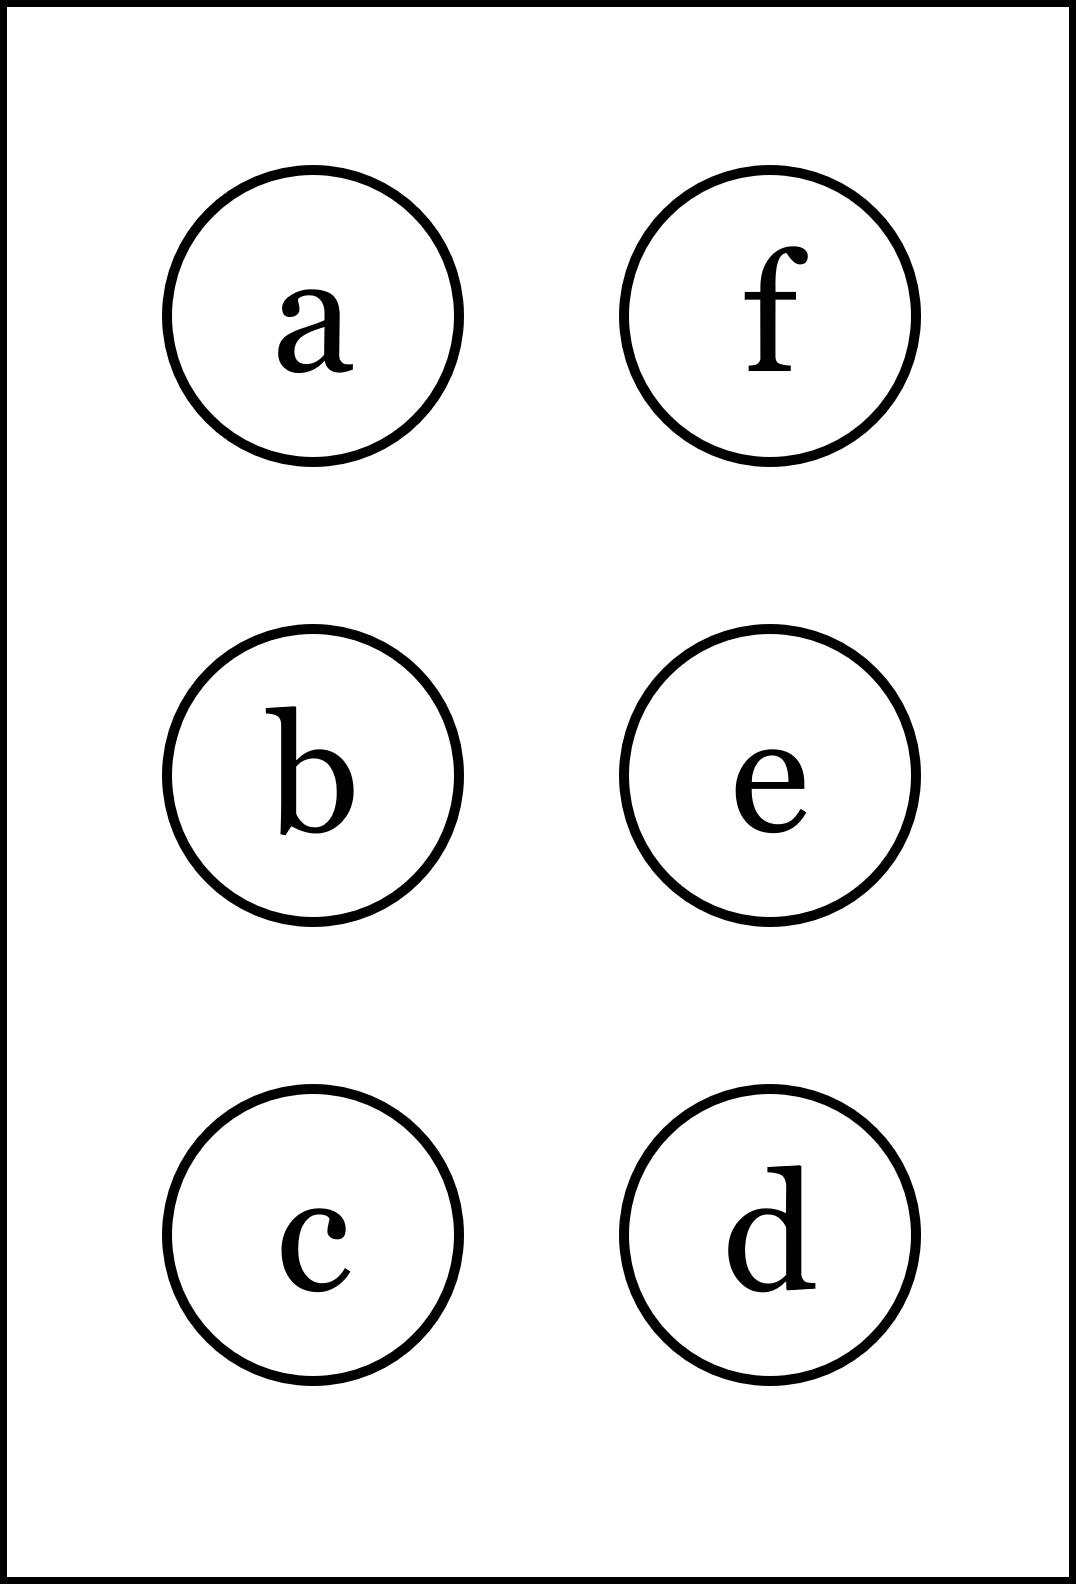
\includegraphics[height=40mm]{../images/braille.png}
{\small Písmeno Braillovej abecedy}
\end{center}
\end{minipage}
\end{center}
\end{minipage}
&
\begin{minipage}[c][104.5mm][t]{0.5\linewidth}
\begin{center}
\vspace{7mm}
{\huge Limity, skupina \textit{Gamma $\gamma$} -\romannumeral4}\\[5mm]
\textit{Meno:}\phantom{xxxxxxxxxxxxxxxxxxxxxxxxxxxxxxxxxxxxxxxxxxxxxxxxxxxxxxxxxxxxxxxxx}\\[5mm]
\begin{minipage}{0.95\linewidth}
\begin{center}
\textbf{Vypočti limity}. Pokud se výsledky shodujú s tými za otazníky, tak napravo\\obarvi příslušející kroužek načerno. \textbf{Spolu odevzdejte výsledné slovo}.
\end{center}
\end{minipage}
\\[1mm]
\begin{minipage}{0.79\linewidth}
\begin{center}
\begin{varwidth}{\linewidth}
\begin{enumerate}
\normalsize
\item $\lim\limits_{n\to\infty}\cfrac{5-6n}{8-n}$\quad \dotfill\; ???\;\dotfill \quad $6$
\item $\lim\limits_{n\to\infty}\cfrac{-3(-1-4n)}{(2n-9)^2}$\quad \dotfill\; ???\;\dotfill \quad $\infty$
\item $\lim\limits_{n\to\infty}\cfrac{(-1+n)^2}{n^2+n+4}$\quad \dotfill\; ???\;\dotfill \quad $\nicefrac{-1}{4}$
\item $\lim\limits_{n\to\infty}\cfrac{2^{n+4}}{2^{n+1}}$\quad \dotfill\; ???\;\dotfill \quad $0$
\item $\lim\limits_{n\to\infty}\cfrac{\left(\frac{3}{2}\right)^n +4}{n^{6}}$\quad \dotfill\; ???\;\dotfill \quad $0$
\item $\lim\limits_{n\to\infty}\cfrac{-2\cdot 2^{n-1}+16\cdot 4^{n-2}}{-4\cdot 4^{n+2}+8\cdot 2^{n-2}}$\quad \dotfill\; ???\;\dotfill \quad $-16$
\end{enumerate}
\end{varwidth}
\end{center}
\end{minipage}
\begin{minipage}{0.20\linewidth}
\begin{center}
{\Huge\bfseries 4.} \\[2mm]
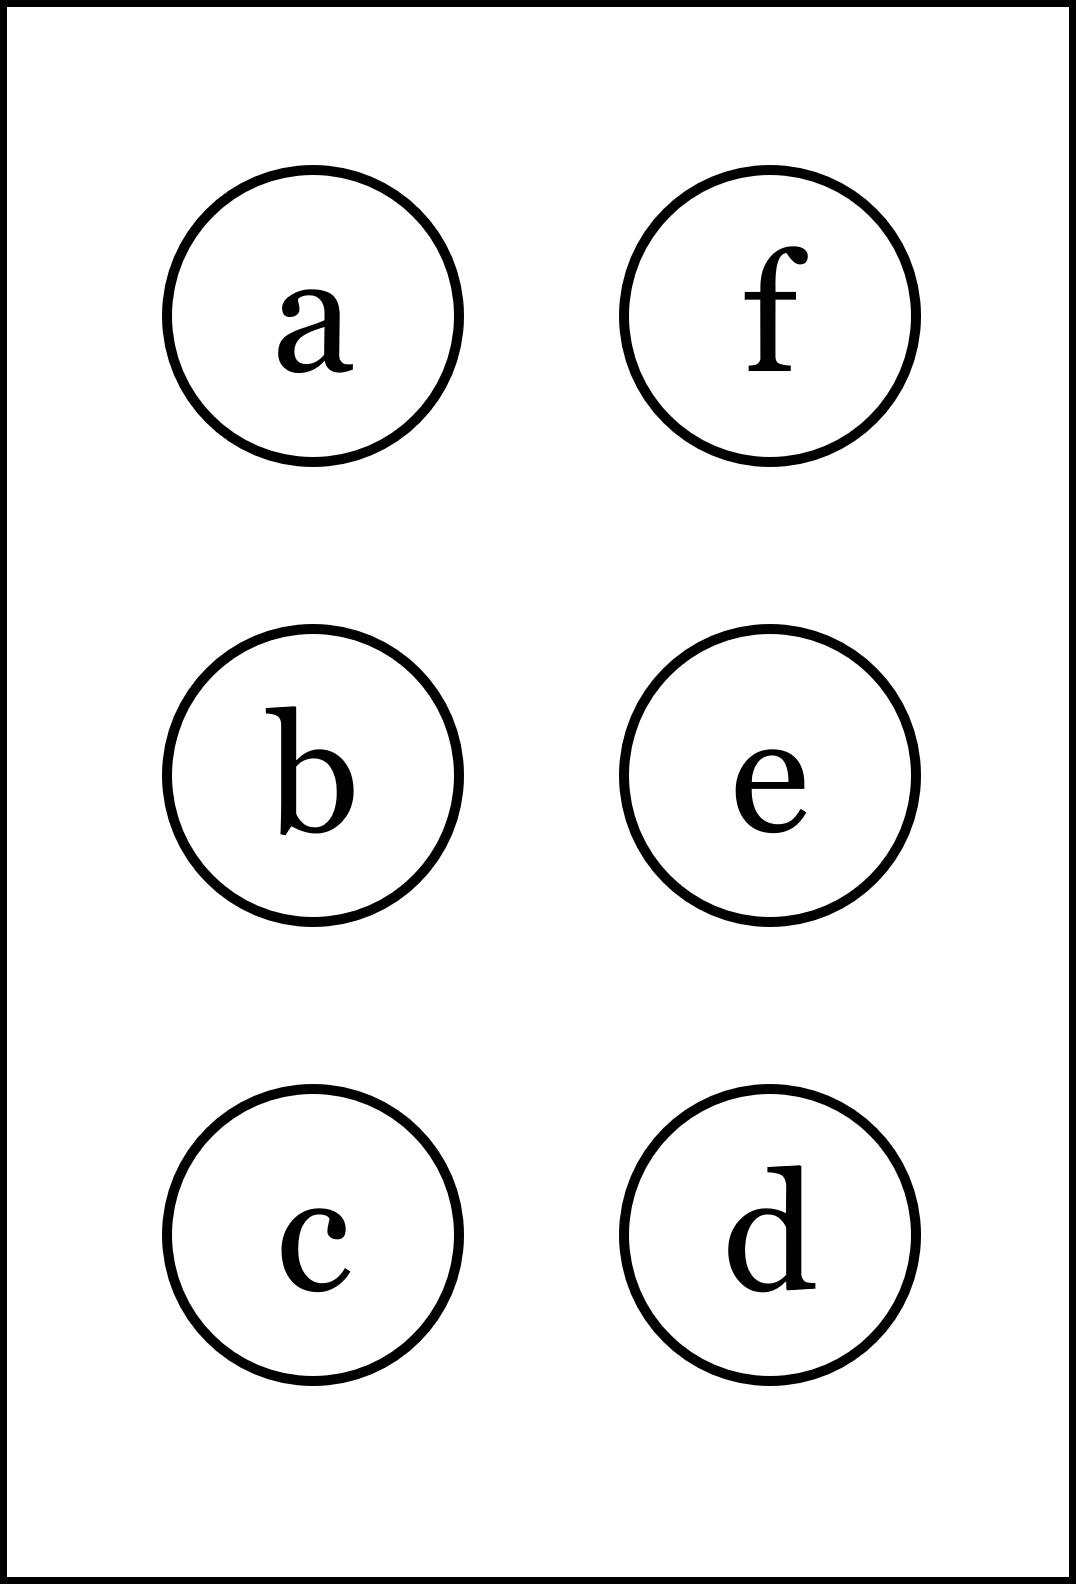
\includegraphics[height=40mm]{../images/braille.png}
{\small Písmeno Braillovej abecedy}
\end{center}
\end{minipage}
\end{center}
\end{minipage}
%
\end{tabular}
\newpage
\thispagestyle{empty}
\begin{tabular}{c:c}
\begin{minipage}[c][104.5mm][t]{0.5\linewidth}
\begin{center}
\vspace{7mm}
{\huge Limity, skupina \textit{Delta $\delta$} -\romannumeral1}\\[5mm]
\textit{Meno:}\phantom{xxxxxxxxxxxxxxxxxxxxxxxxxxxxxxxxxxxxxxxxxxxxxxxxxxxxxxxxxxxxxxxxx}\\[5mm]
\begin{minipage}{0.95\linewidth}
\begin{center}
\textbf{Vypočti limity}. Pokud se výsledky shodujú s tými za otazníky, tak napravo\\obarvi příslušející kroužek načerno. \textbf{Spolu odevzdejte výsledné slovo}.
\end{center}
\end{minipage}
\\[1mm]
\begin{minipage}{0.79\linewidth}
\begin{center}
\begin{varwidth}{\linewidth}
\begin{enumerate}
\normalsize
\item $\lim\limits_{n\to\infty}\cfrac{7+5n}{3-7n}$\quad \dotfill\; ???\;\dotfill \quad $\nicefrac{-5}{7}$
\item $\lim\limits_{n\to\infty}\cfrac{-9(1+2n)}{(-2n+3)^2}$\quad \dotfill\; ???\;\dotfill \quad $\infty$
\item $\lim\limits_{n\to\infty}\cfrac{(-1+6n)^2}{n^2+5n+4}$\quad \dotfill\; ???\;\dotfill \quad $36$
\item $\lim\limits_{n\to\infty}\cfrac{2^{n+1}}{2^{n-3}}$\quad \dotfill\; ???\;\dotfill \quad $2$
\item $\lim\limits_{n\to\infty}\cfrac{\left(\frac{1}{2}\right)^n -2}{-n^{6}}$\quad \dotfill\; ???\;\dotfill \quad $0$
\item $\lim\limits_{n\to\infty}\cfrac{-3\cdot 3^{n+2}-9\cdot 4^{n-1}}{3\cdot 4^{n-2}-16\cdot 3^{n-2}}$\quad \dotfill\; ???\;\dotfill \quad $\nicefrac{-3}{4}$
\end{enumerate}
\end{varwidth}
\end{center}
\end{minipage}
\begin{minipage}{0.20\linewidth}
\begin{center}
{\Huge\bfseries 1.} \\[2mm]
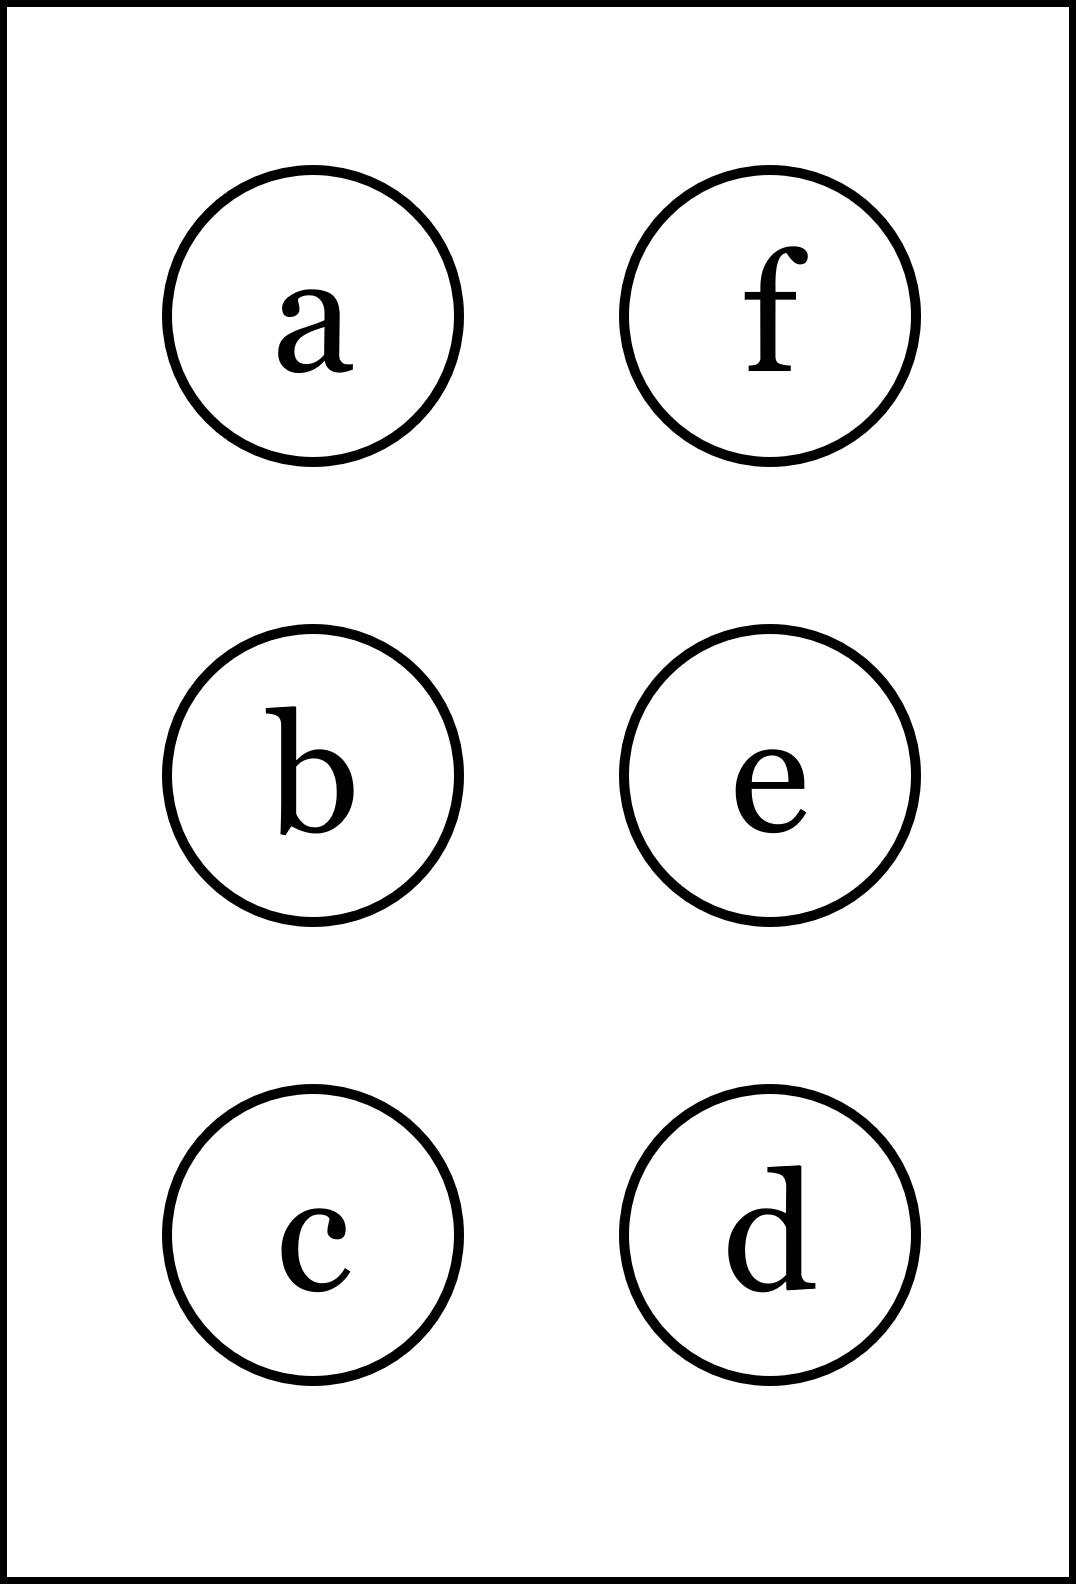
\includegraphics[height=40mm]{../images/braille.png}
{\small Písmeno Braillovej abecedy}
\end{center}
\end{minipage}
\end{center}
\end{minipage}
&
\begin{minipage}[c][104.5mm][t]{0.5\linewidth}
\begin{center}
\vspace{7mm}
{\huge Limity, skupina \textit{Delta $\delta$} -\romannumeral2}\\[5mm]
\textit{Meno:}\phantom{xxxxxxxxxxxxxxxxxxxxxxxxxxxxxxxxxxxxxxxxxxxxxxxxxxxxxxxxxxxxxxxxx}\\[5mm]
\begin{minipage}{0.95\linewidth}
\begin{center}
\textbf{Vypočti limity}. Pokud se výsledky shodujú s tými za otazníky, tak napravo\\obarvi příslušející kroužek načerno. \textbf{Spolu odevzdejte výsledné slovo}.
\end{center}
\end{minipage}
\\[1mm]
\begin{minipage}{0.79\linewidth}
\begin{center}
\begin{varwidth}{\linewidth}
\begin{enumerate}
\normalsize
\item $\lim\limits_{n\to\infty}\cfrac{-2+3n}{2+4n}$\quad \dotfill\; ???\;\dotfill \quad $0$
\item $\lim\limits_{n\to\infty}\cfrac{-3(-3+4n)}{(3n-1)^2}$\quad \dotfill\; ???\;\dotfill \quad $0$
\item $\lim\limits_{n\to\infty}\cfrac{(-7+n)^2}{n^2+8n+4}$\quad \dotfill\; ???\;\dotfill \quad $1$
\item $\lim\limits_{n\to\infty}\cfrac{4^{n+2}}{4^{n+4}}$\quad \dotfill\; ???\;\dotfill \quad $\infty$
\item $\lim\limits_{n\to\infty}\cfrac{\left(\frac{2}{4}\right)^n -3}{-4n^{6}}$\quad \dotfill\; ???\;\dotfill \quad $-\infty$
\item $\lim\limits_{n\to\infty}\cfrac{8\cdot 2^{n+1}+16\cdot 4^{n-2}}{-2\cdot 4^{n-2}+8\cdot 2^{n-1}}$\quad \dotfill\; ???\;\dotfill \quad $-8$
\end{enumerate}
\end{varwidth}
\end{center}
\end{minipage}
\begin{minipage}{0.20\linewidth}
\begin{center}
{\Huge\bfseries 2.} \\[2mm]
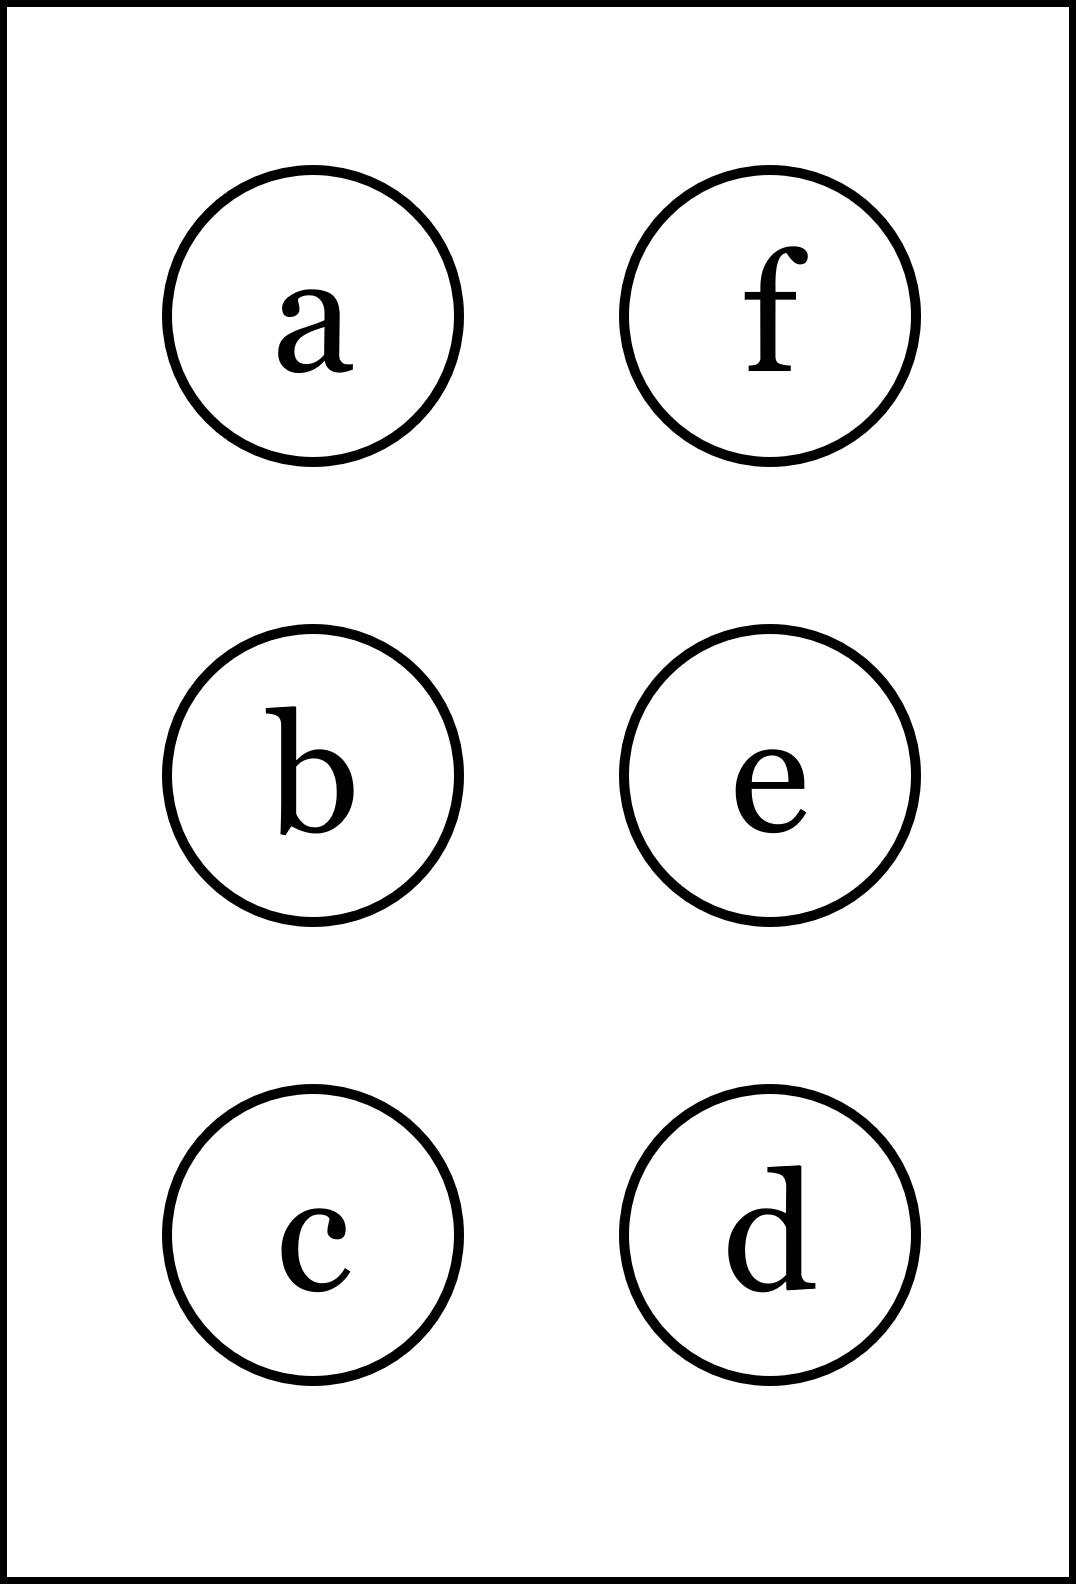
\includegraphics[height=40mm]{../images/braille.png}
{\small Písmeno Braillovej abecedy}
\end{center}
\end{minipage}
\end{center}
\end{minipage}
\\ \hdashline
\begin{minipage}[c][104.5mm][t]{0.5\linewidth}
\begin{center}
\vspace{7mm}
{\huge Limity, skupina \textit{Delta $\delta$} -\romannumeral3}\\[5mm]
\textit{Meno:}\phantom{xxxxxxxxxxxxxxxxxxxxxxxxxxxxxxxxxxxxxxxxxxxxxxxxxxxxxxxxxxxxxxxxx}\\[5mm]
\begin{minipage}{0.95\linewidth}
\begin{center}
\textbf{Vypočti limity}. Pokud se výsledky shodujú s tými za otazníky, tak napravo\\obarvi příslušející kroužek načerno. \textbf{Spolu odevzdejte výsledné slovo}.
\end{center}
\end{minipage}
\\[1mm]
\begin{minipage}{0.79\linewidth}
\begin{center}
\begin{varwidth}{\linewidth}
\begin{enumerate}
\normalsize
\item $\lim\limits_{n\to\infty}\cfrac{-4-5n}{-1-5n}$\quad \dotfill\; ???\;\dotfill \quad $1$
\item $\lim\limits_{n\to\infty}\cfrac{1(2+6n)}{(-6n-5)^2}$\quad \dotfill\; ???\;\dotfill \quad $-1$
\item $\lim\limits_{n\to\infty}\cfrac{(-5+n)^2}{n^2-4n+6}$\quad \dotfill\; ???\;\dotfill \quad $0$
\item $\lim\limits_{n\to\infty}\cfrac{2^{n-1}}{2^{n-3}}$\quad \dotfill\; ???\;\dotfill \quad $\infty$
\item $\lim\limits_{n\to\infty}\cfrac{\left(\frac{1}{2}\right)^n +1}{n^{12}}$\quad \dotfill\; ???\;\dotfill \quad $0$
\item $\lim\limits_{n\to\infty}\cfrac{8\cdot 2^{n+1}-16\cdot 4^{n-1}}{16\cdot 4^{n+1}+2\cdot 2^{n+2}}$\quad \dotfill\; ???\;\dotfill \quad $-4$
\end{enumerate}
\end{varwidth}
\end{center}
\end{minipage}
\begin{minipage}{0.20\linewidth}
\begin{center}
{\Huge\bfseries 3.} \\[2mm]
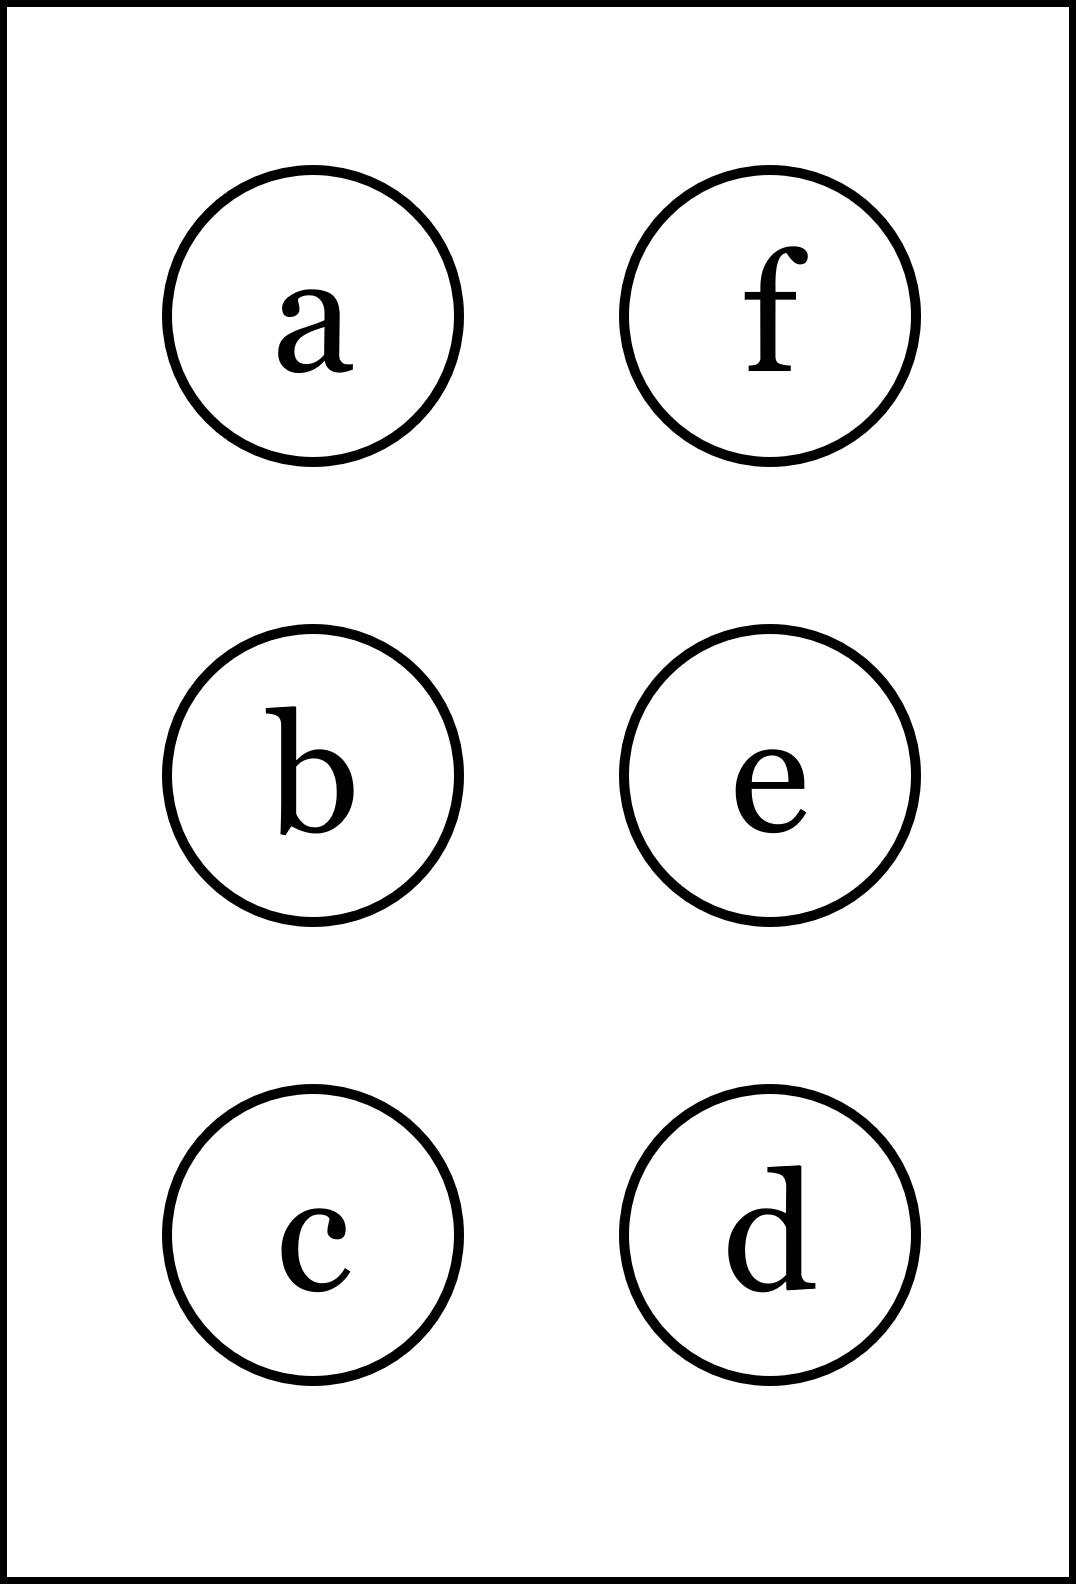
\includegraphics[height=40mm]{../images/braille.png}
{\small Písmeno Braillovej abecedy}
\end{center}
\end{minipage}
\end{center}
\end{minipage}
&
\begin{minipage}[c][104.5mm][t]{0.5\linewidth}
\begin{center}
\vspace{7mm}
{\huge Limity, skupina \textit{Delta $\delta$} -\romannumeral4}\\[5mm]
\textit{Meno:}\phantom{xxxxxxxxxxxxxxxxxxxxxxxxxxxxxxxxxxxxxxxxxxxxxxxxxxxxxxxxxxxxxxxxx}\\[5mm]
\begin{minipage}{0.95\linewidth}
\begin{center}
\textbf{Vypočti limity}. Pokud se výsledky shodujú s tými za otazníky, tak napravo\\obarvi příslušející kroužek načerno. \textbf{Spolu odevzdejte výsledné slovo}.
\end{center}
\end{minipage}
\\[1mm]
\begin{minipage}{0.79\linewidth}
\begin{center}
\begin{varwidth}{\linewidth}
\begin{enumerate}
\normalsize
\item $\lim\limits_{n\to\infty}\cfrac{7+8n}{4-4n}$\quad \dotfill\; ???\;\dotfill \quad $-2$
\item $\lim\limits_{n\to\infty}\cfrac{4(1-8n)}{(-3n+5)^2}$\quad \dotfill\; ???\;\dotfill \quad $0$
\item $\lim\limits_{n\to\infty}\cfrac{(-5-3n)^2}{n^2-4n+5}$\quad \dotfill\; ???\;\dotfill \quad $9$
\item $\lim\limits_{n\to\infty}\cfrac{3^{n-2}}{3^{n-1}}$\quad \dotfill\; ???\;\dotfill \quad $0$
\item $\lim\limits_{n\to\infty}\cfrac{\left(\frac{1}{4}\right)^n -3}{n^{-8}}$\quad \dotfill\; ???\;\dotfill \quad $-3$
\item $\lim\limits_{n\to\infty}\cfrac{-6\cdot 2^{n+1}+9\cdot 3^{n-2}}{-4\cdot 3^{n-2}+2\cdot 2^{n+2}}$\quad \dotfill\; ???\;\dotfill \quad $\nicefrac{-9}{8}$
\end{enumerate}
\end{varwidth}
\end{center}
\end{minipage}
\begin{minipage}{0.20\linewidth}
\begin{center}
{\Huge\bfseries 4.} \\[2mm]
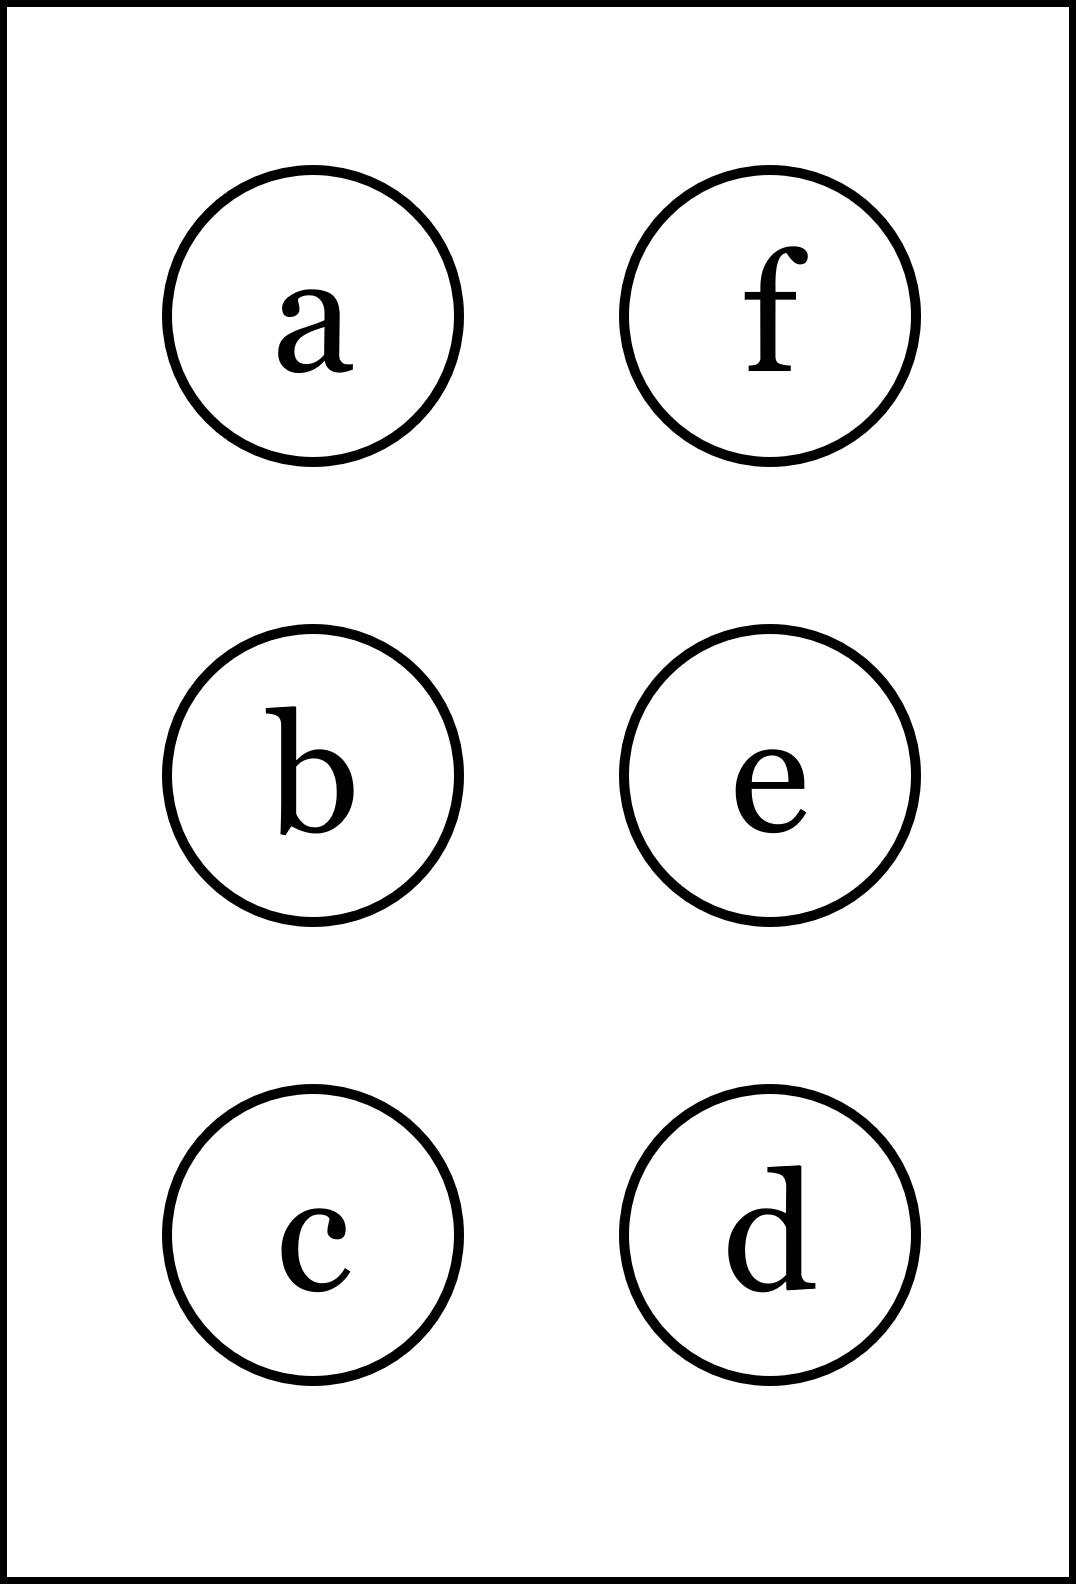
\includegraphics[height=40mm]{../images/braille.png}
{\small Písmeno Braillovej abecedy}
\end{center}
\end{minipage}
\end{center}
\end{minipage}
%
\end{tabular}
\newpage
\thispagestyle{empty}
\begin{tabular}{c:c}
\begin{minipage}[c][104.5mm][t]{0.5\linewidth}
\begin{center}
\vspace{7mm}
{\huge Limity, skupina \textit{Epsilon $\epsilon$} -\romannumeral1}\\[5mm]
\textit{Meno:}\phantom{xxxxxxxxxxxxxxxxxxxxxxxxxxxxxxxxxxxxxxxxxxxxxxxxxxxxxxxxxxxxxxxxx}\\[5mm]
\begin{minipage}{0.95\linewidth}
\begin{center}
\textbf{Vypočti limity}. Pokud se výsledky shodujú s tými za otazníky, tak napravo\\obarvi příslušející kroužek načerno. \textbf{Spolu odevzdejte výsledné slovo}.
\end{center}
\end{minipage}
\\[1mm]
\begin{minipage}{0.79\linewidth}
\begin{center}
\begin{varwidth}{\linewidth}
\begin{enumerate}
\normalsize
\item $\lim\limits_{n\to\infty}\cfrac{-2-6n}{4+9n}$\quad \dotfill\; ???\;\dotfill \quad $\nicefrac{-2}{3}$
\item $\lim\limits_{n\to\infty}\cfrac{3(-2+3n)}{(6n+3)^2}$\quad \dotfill\; ???\;\dotfill \quad $0$
\item $\lim\limits_{n\to\infty}\cfrac{(-2-2n)^2}{n^2-8n+2}$\quad \dotfill\; ???\;\dotfill \quad $4$
\item $\lim\limits_{n\to\infty}\cfrac{3^{n+2}}{3^{n+3}}$\quad \dotfill\; ???\;\dotfill \quad $\nicefrac{1}{3}$
\item $\lim\limits_{n\to\infty}\cfrac{\left(\frac{4}{2}\right)^n +2}{-3n^{-12}}$\quad \dotfill\; ???\;\dotfill \quad $-\infty$
\item $\lim\limits_{n\to\infty}\cfrac{-3\cdot 3^{n+1}-16\cdot 4^{n-1}}{4\cdot 4^{n+1}-4\cdot 3^{n+2}}$\quad \dotfill\; ???\;\dotfill \quad $-16$
\end{enumerate}
\end{varwidth}
\end{center}
\end{minipage}
\begin{minipage}{0.20\linewidth}
\begin{center}
{\Huge\bfseries 1.} \\[2mm]
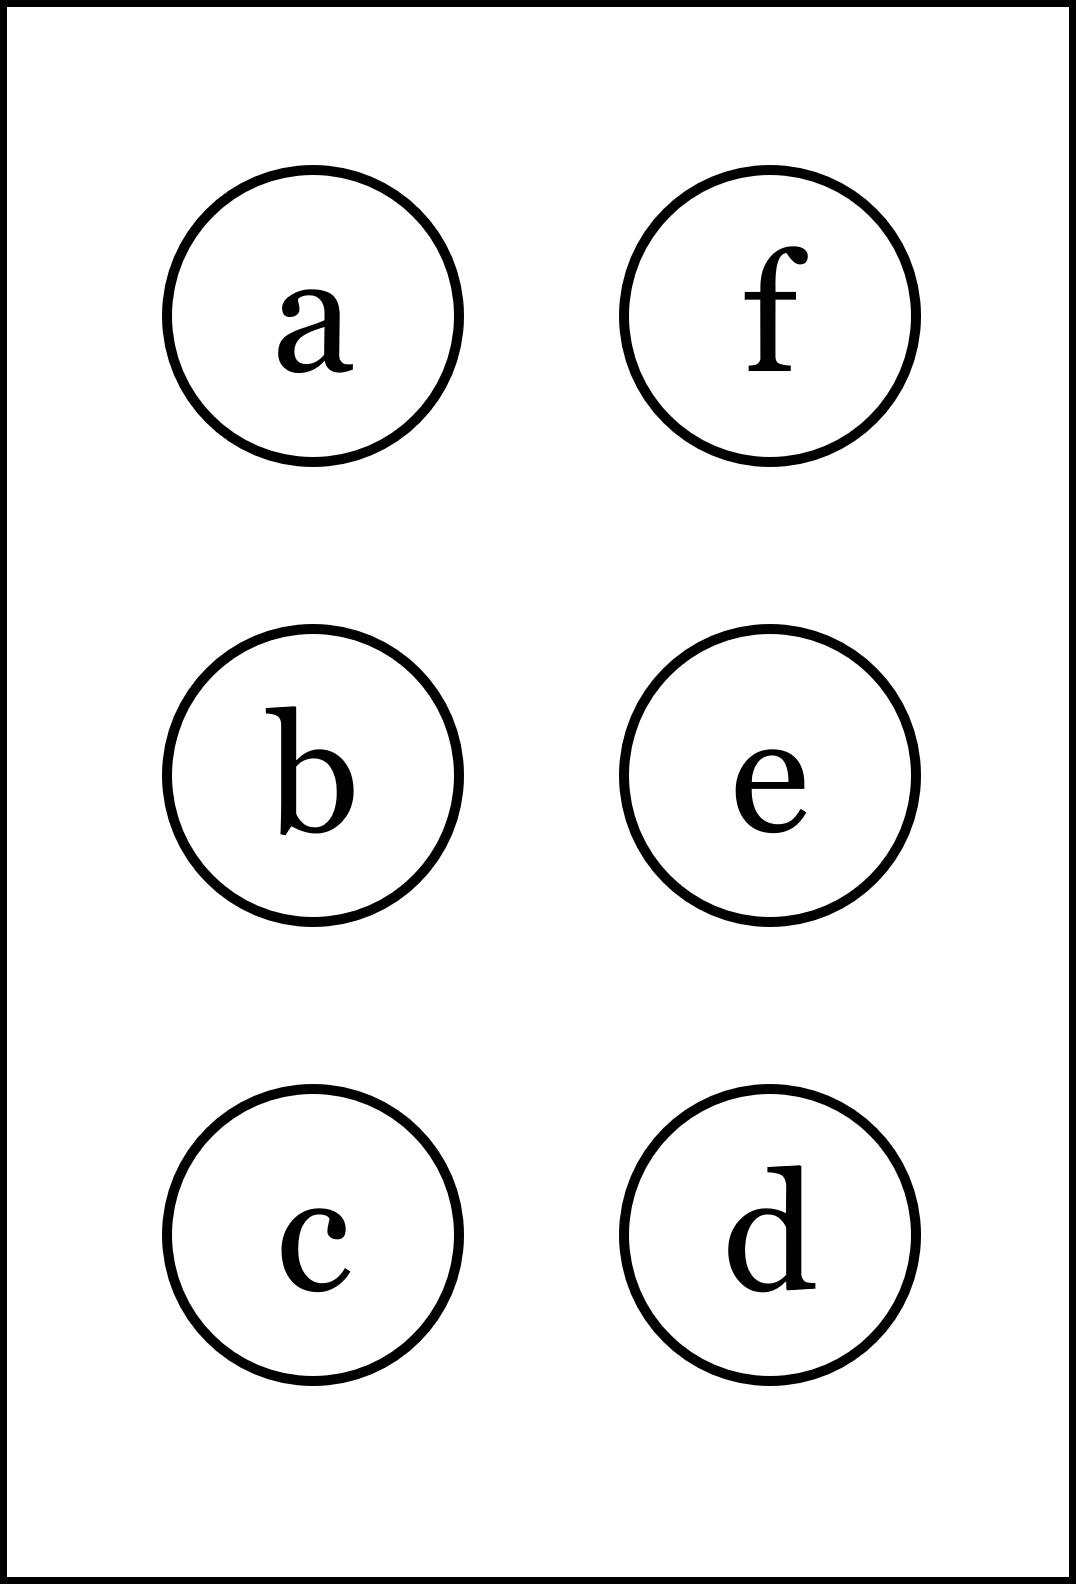
\includegraphics[height=40mm]{../images/braille.png}
{\small Písmeno Braillovej abecedy}
\end{center}
\end{minipage}
\end{center}
\end{minipage}
&
\begin{minipage}[c][104.5mm][t]{0.5\linewidth}
\begin{center}
\vspace{7mm}
{\huge Limity, skupina \textit{Epsilon $\epsilon$} -\romannumeral2}\\[5mm]
\textit{Meno:}\phantom{xxxxxxxxxxxxxxxxxxxxxxxxxxxxxxxxxxxxxxxxxxxxxxxxxxxxxxxxxxxxxxxxx}\\[5mm]
\begin{minipage}{0.95\linewidth}
\begin{center}
\textbf{Vypočti limity}. Pokud se výsledky shodujú s tými za otazníky, tak napravo\\obarvi příslušející kroužek načerno. \textbf{Spolu odevzdejte výsledné slovo}.
\end{center}
\end{minipage}
\\[1mm]
\begin{minipage}{0.79\linewidth}
\begin{center}
\begin{varwidth}{\linewidth}
\begin{enumerate}
\normalsize
\item $\lim\limits_{n\to\infty}\cfrac{-7+4n}{-6-8n}$\quad \dotfill\; ???\;\dotfill \quad $\nicefrac{-1}{2}$
\item $\lim\limits_{n\to\infty}\cfrac{3(-1+8n)}{(-n-4)^2}$\quad \dotfill\; ???\;\dotfill \quad $-\infty$
\item $\lim\limits_{n\to\infty}\cfrac{(1-4n)^2}{n^2+n+4}$\quad \dotfill\; ???\;\dotfill \quad $\infty$
\item $\lim\limits_{n\to\infty}\cfrac{2^{n+1}}{2^{n+2}}$\quad \dotfill\; ???\;\dotfill \quad $-\infty$
\item $\lim\limits_{n\to\infty}\cfrac{\left(\frac{2}{3}\right)^n +3}{-2n^{-8}}$\quad \dotfill\; ???\;\dotfill \quad $0$
\item $\lim\limits_{n\to\infty}\cfrac{-4\cdot 2^{n-2}-4\cdot 4^{n+1}}{16\cdot 4^{n-2}+4\cdot 2^{n-2}}$\quad \dotfill\; ???\;\dotfill \quad $\nicefrac{-1}{16}$
\end{enumerate}
\end{varwidth}
\end{center}
\end{minipage}
\begin{minipage}{0.20\linewidth}
\begin{center}
{\Huge\bfseries 2.} \\[2mm]
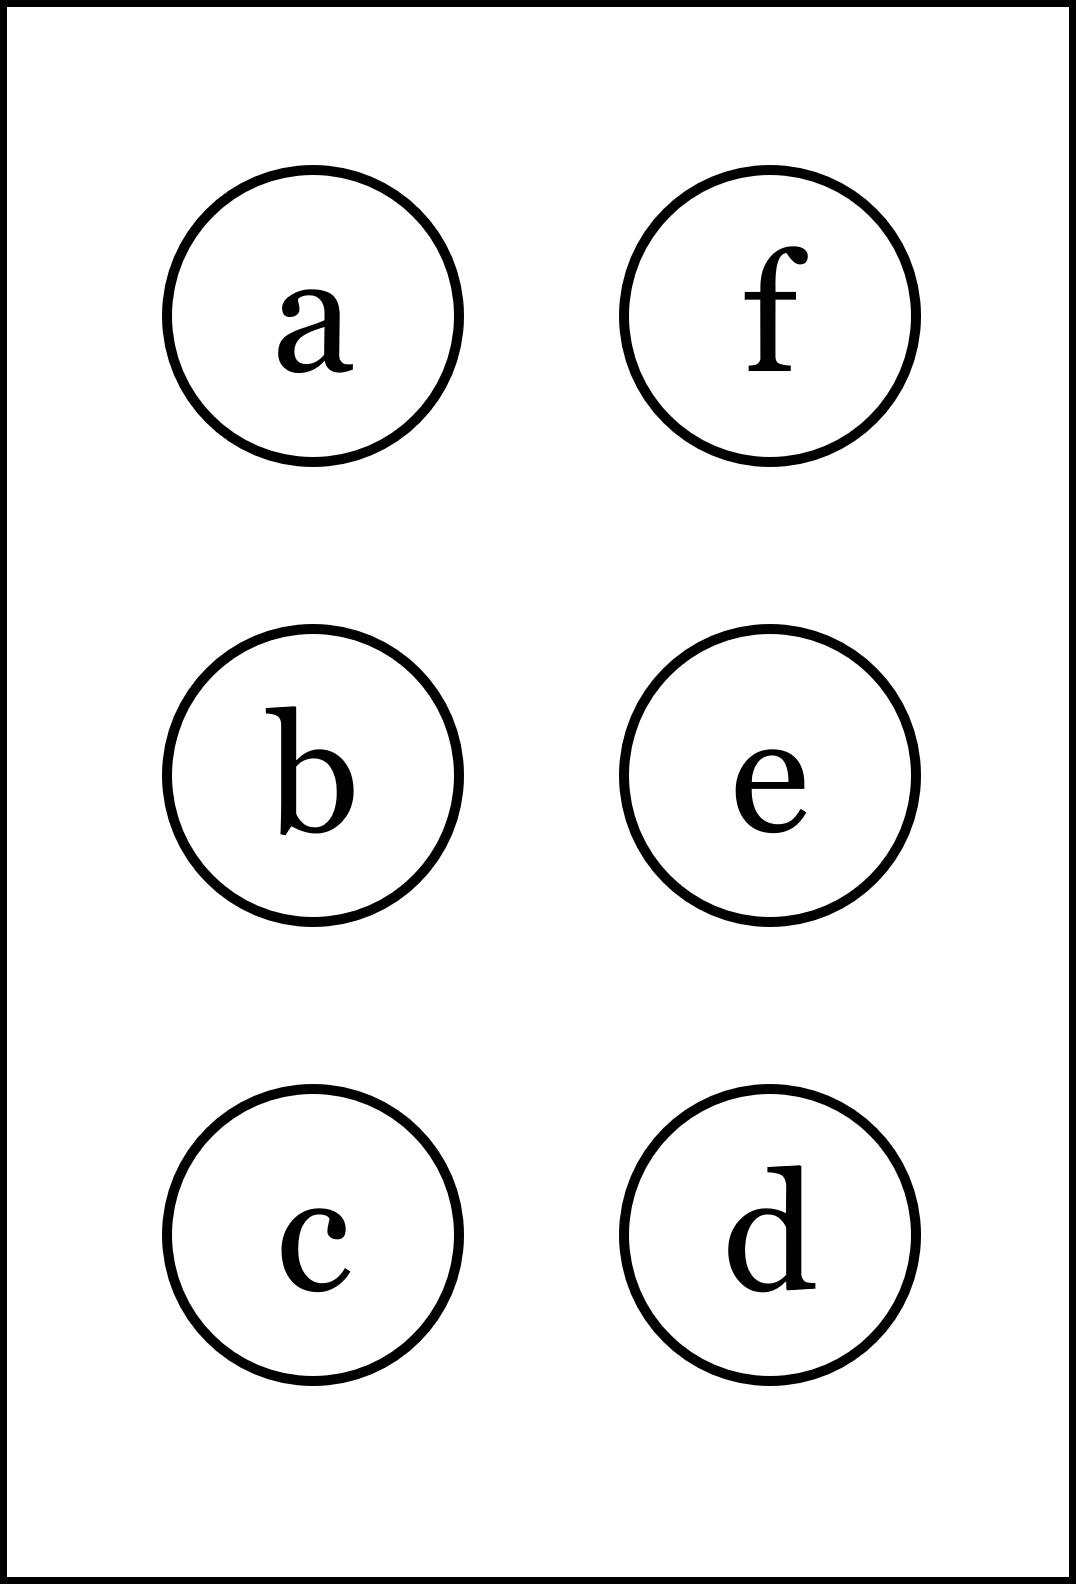
\includegraphics[height=40mm]{../images/braille.png}
{\small Písmeno Braillovej abecedy}
\end{center}
\end{minipage}
\end{center}
\end{minipage}
\\ \hdashline
\begin{minipage}[c][104.5mm][t]{0.5\linewidth}
\begin{center}
\vspace{7mm}
{\huge Limity, skupina \textit{Epsilon $\epsilon$} -\romannumeral3}\\[5mm]
\textit{Meno:}\phantom{xxxxxxxxxxxxxxxxxxxxxxxxxxxxxxxxxxxxxxxxxxxxxxxxxxxxxxxxxxxxxxxxx}\\[5mm]
\begin{minipage}{0.95\linewidth}
\begin{center}
\textbf{Vypočti limity}. Pokud se výsledky shodujú s tými za otazníky, tak napravo\\obarvi příslušející kroužek načerno. \textbf{Spolu odevzdejte výsledné slovo}.
\end{center}
\end{minipage}
\\[1mm]
\begin{minipage}{0.79\linewidth}
\begin{center}
\begin{varwidth}{\linewidth}
\begin{enumerate}
\normalsize
\item $\lim\limits_{n\to\infty}\cfrac{2+n}{2-3n}$\quad \dotfill\; ???\;\dotfill \quad $\infty$
\item $\lim\limits_{n\to\infty}\cfrac{-2(-7+9n)}{(-n+8)^2}$\quad \dotfill\; ???\;\dotfill \quad $0$
\item $\lim\limits_{n\to\infty}\cfrac{(7+n)^2}{n^2+2n-9}$\quad \dotfill\; ???\;\dotfill \quad $1$
\item $\lim\limits_{n\to\infty}\cfrac{3^{n+2}}{3^{n-2}}$\quad \dotfill\; ???\;\dotfill \quad $9$
\item $\lim\limits_{n\to\infty}\cfrac{\left(\frac{1}{3}\right)^n +2}{3n^{8}}$\quad \dotfill\; ???\;\dotfill \quad $0$
\item $\lim\limits_{n\to\infty}\cfrac{-2\cdot 2^{n+1}-2\cdot 3^{n-2}}{-6\cdot 3^{n+2}-2\cdot 2^{n+1}}$\quad \dotfill\; ???\;\dotfill \quad $\nicefrac{1}{243}$
\end{enumerate}
\end{varwidth}
\end{center}
\end{minipage}
\begin{minipage}{0.20\linewidth}
\begin{center}
{\Huge\bfseries 3.} \\[2mm]
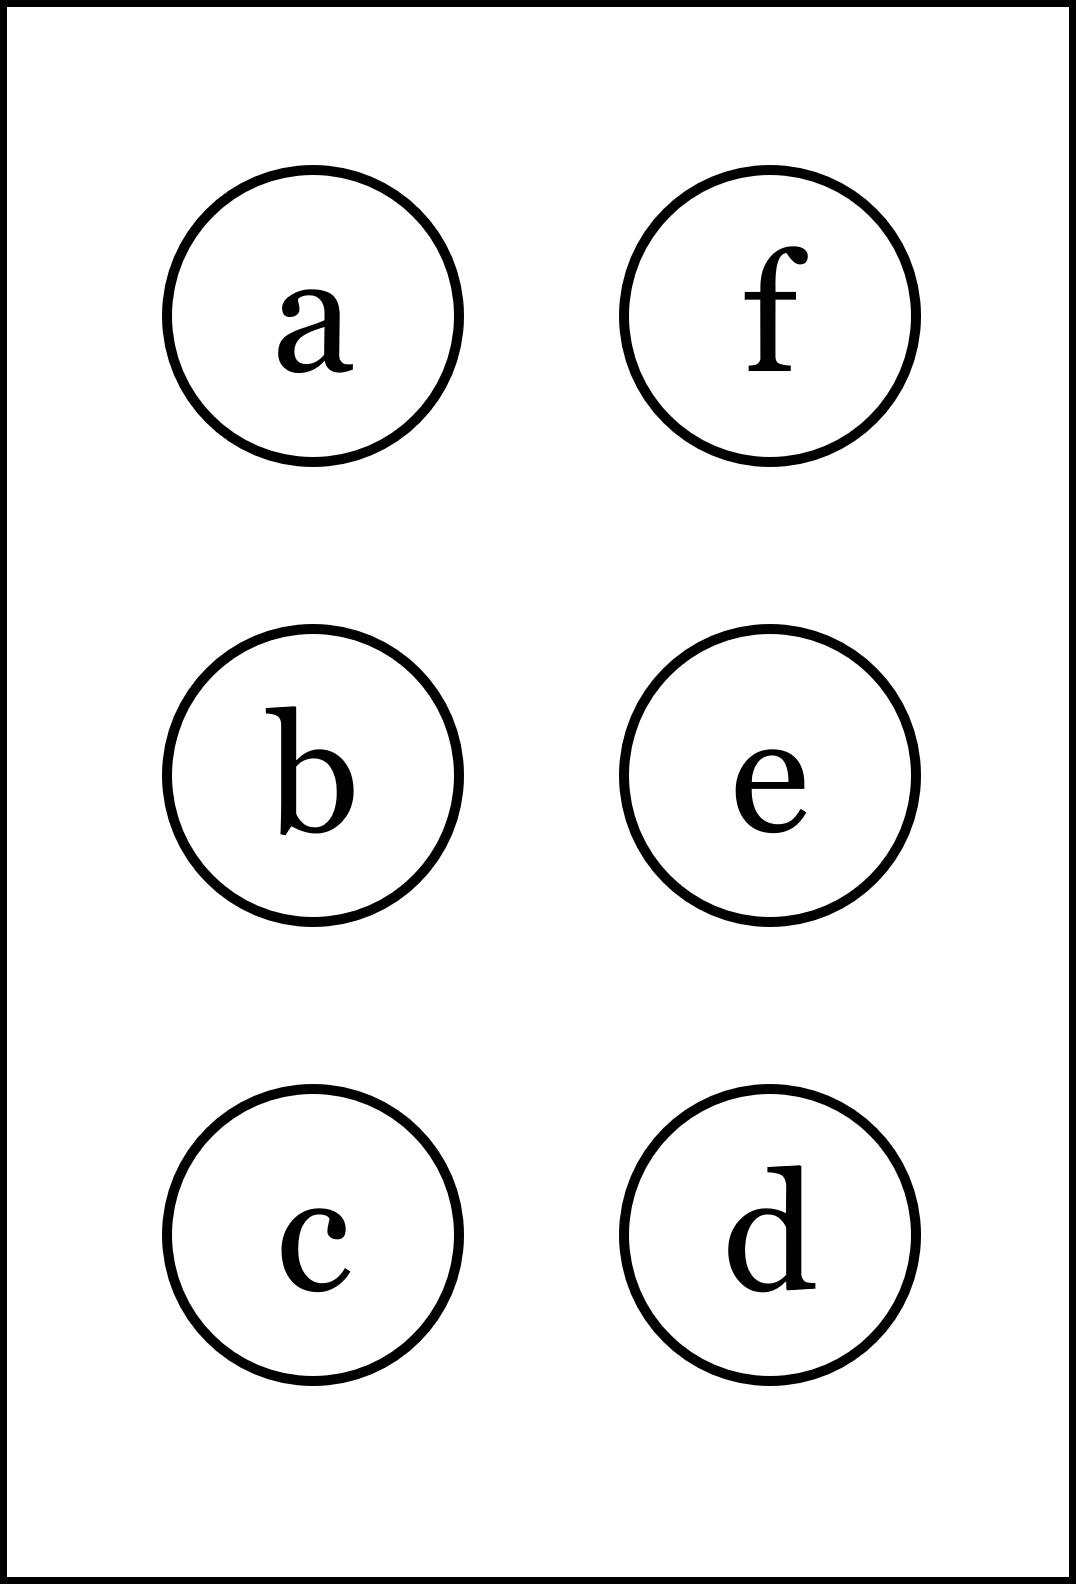
\includegraphics[height=40mm]{../images/braille.png}
{\small Písmeno Braillovej abecedy}
\end{center}
\end{minipage}
\end{center}
\end{minipage}
&
\begin{minipage}[c][104.5mm][t]{0.5\linewidth}
\begin{center}
\vspace{7mm}
{\huge Limity, skupina \textit{Epsilon $\epsilon$} -\romannumeral4}\\[5mm]
\textit{Meno:}\phantom{xxxxxxxxxxxxxxxxxxxxxxxxxxxxxxxxxxxxxxxxxxxxxxxxxxxxxxxxxxxxxxxxx}\\[5mm]
\begin{minipage}{0.95\linewidth}
\begin{center}
\textbf{Vypočti limity}. Pokud se výsledky shodujú s tými za otazníky, tak napravo\\obarvi příslušející kroužek načerno. \textbf{Spolu odevzdejte výsledné slovo}.
\end{center}
\end{minipage}
\\[1mm]
\begin{minipage}{0.79\linewidth}
\begin{center}
\begin{varwidth}{\linewidth}
\begin{enumerate}
\normalsize
\item $\lim\limits_{n\to\infty}\cfrac{-1-3n}{-3+3n}$\quad \dotfill\; ???\;\dotfill \quad $0$
\item $\lim\limits_{n\to\infty}\cfrac{4(4+6n)}{(3n+2)^2}$\quad \dotfill\; ???\;\dotfill \quad $0$
\item $\lim\limits_{n\to\infty}\cfrac{(2-4n)^2}{n^2-n+6}$\quad \dotfill\; ???\;\dotfill \quad $16$
\item $\lim\limits_{n\to\infty}\cfrac{4^{n+1}}{4^{n+1}}$\quad \dotfill\; ???\;\dotfill \quad $-\infty$
\item $\lim\limits_{n\to\infty}\cfrac{\left(\frac{3}{2}\right)^n -3}{-2n^{-6}}$\quad \dotfill\; ???\;\dotfill \quad $-\infty$
\item $\lim\limits_{n\to\infty}\cfrac{2\cdot 2^{n+2}+6\cdot 3^{n-2}}{2\cdot 3^{n-2}-6\cdot 2^{n-1}}$\quad \dotfill\; ???\;\dotfill \quad $3$
\end{enumerate}
\end{varwidth}
\end{center}
\end{minipage}
\begin{minipage}{0.20\linewidth}
\begin{center}
{\Huge\bfseries 4.} \\[2mm]
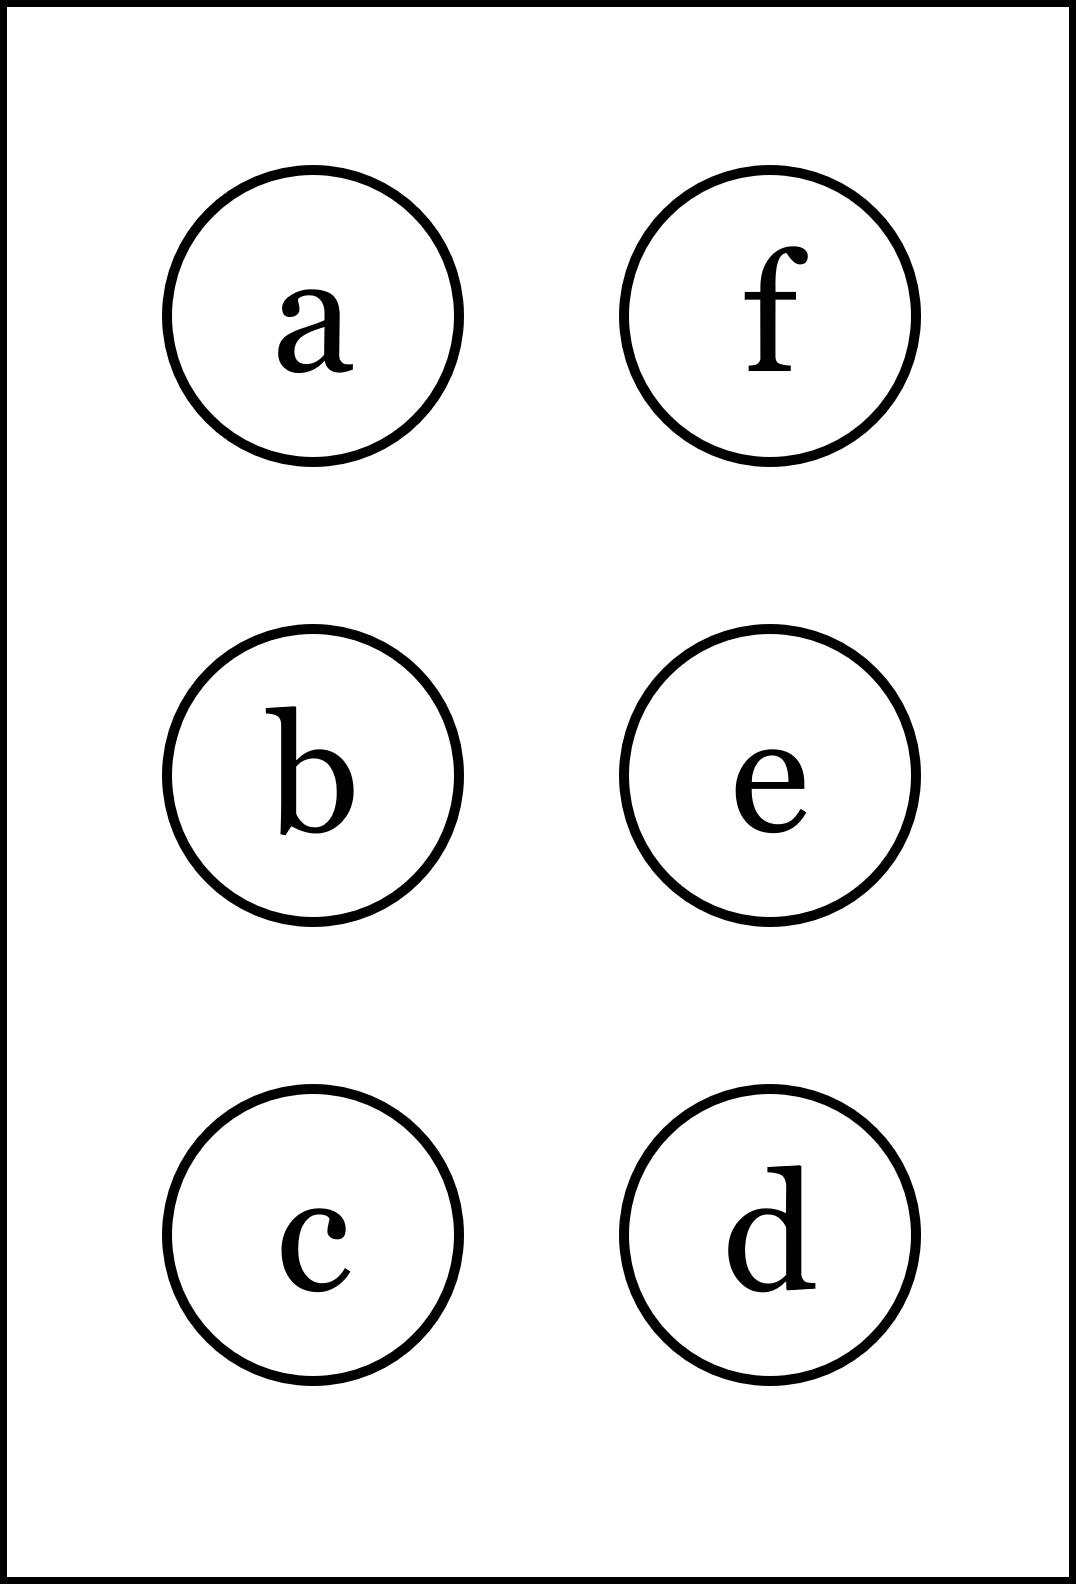
\includegraphics[height=40mm]{../images/braille.png}
{\small Písmeno Braillovej abecedy}
\end{center}
\end{minipage}
\end{center}
\end{minipage}
%
\end{tabular}
\newpage
\thispagestyle{empty}
\begin{tabular}{c:c}
\begin{minipage}[c][104.5mm][t]{0.5\linewidth}
\begin{center}
\vspace{7mm}
{\huge Limity, skupina \textit{Zeta $\zeta$} -\romannumeral1}\\[5mm]
\textit{Meno:}\phantom{xxxxxxxxxxxxxxxxxxxxxxxxxxxxxxxxxxxxxxxxxxxxxxxxxxxxxxxxxxxxxxxxx}\\[5mm]
\begin{minipage}{0.95\linewidth}
\begin{center}
\textbf{Vypočti limity}. Pokud se výsledky shodujú s tými za otazníky, tak napravo\\obarvi příslušející kroužek načerno. \textbf{Spolu odevzdejte výsledné slovo}.
\end{center}
\end{minipage}
\\[1mm]
\begin{minipage}{0.79\linewidth}
\begin{center}
\begin{varwidth}{\linewidth}
\begin{enumerate}
\normalsize
\item $\lim\limits_{n\to\infty}\cfrac{-1+n}{2-n}$\quad \dotfill\; ???\;\dotfill \quad $-1$
\item $\lim\limits_{n\to\infty}\cfrac{4(-5+7n)}{(n-2)^2}$\quad \dotfill\; ???\;\dotfill \quad $\nicefrac{-7}{4}$
\item $\lim\limits_{n\to\infty}\cfrac{(-9-6n)^2}{n^2+3n-4}$\quad \dotfill\; ???\;\dotfill \quad $-\infty$
\item $\lim\limits_{n\to\infty}\cfrac{3^{n-3}}{3^{n-4}}$\quad \dotfill\; ???\;\dotfill \quad $-\infty$
\item $\lim\limits_{n\to\infty}\cfrac{\left(\frac{1}{2}\right)^n -1}{-2n^{12}}$\quad \dotfill\; ???\;\dotfill \quad $0$
\item $\lim\limits_{n\to\infty}\cfrac{-4\cdot 2^{n+1}+4\cdot 4^{n-2}}{8\cdot 4^{n-1}-8\cdot 2^{n+1}}$\quad \dotfill\; ???\;\dotfill \quad $2$
\end{enumerate}
\end{varwidth}
\end{center}
\end{minipage}
\begin{minipage}{0.20\linewidth}
\begin{center}
{\Huge\bfseries 1.} \\[2mm]
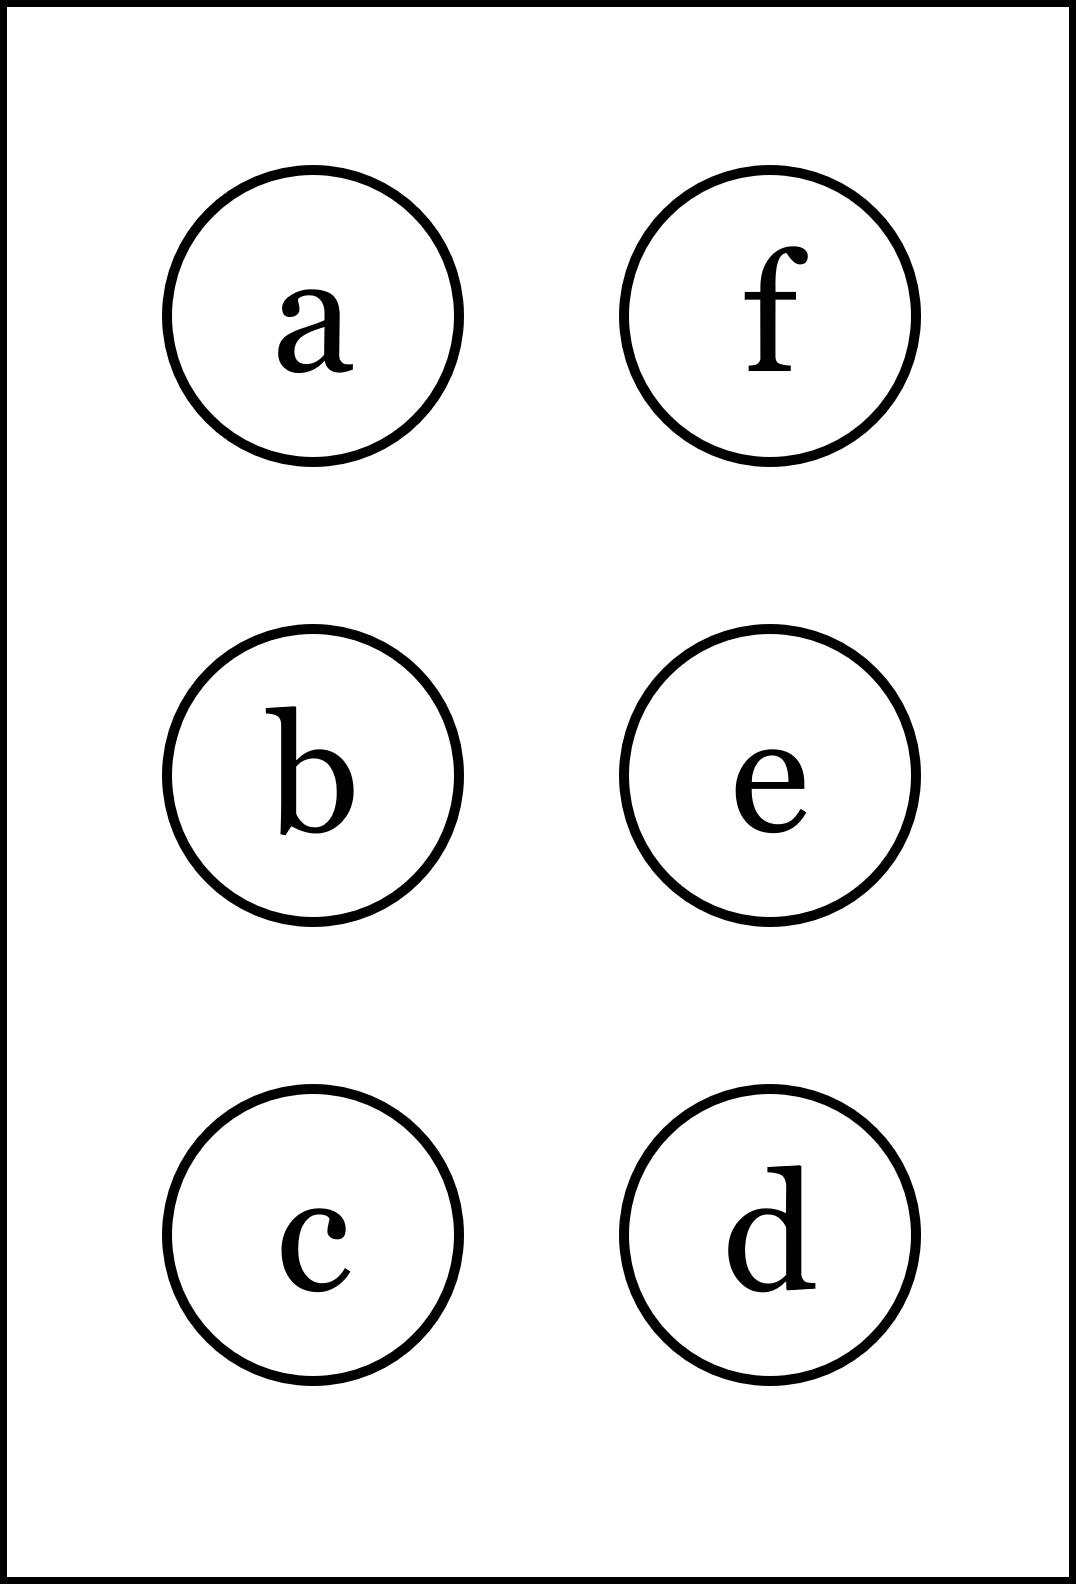
\includegraphics[height=40mm]{../images/braille.png}
{\small Písmeno Braillovej abecedy}
\end{center}
\end{minipage}
\end{center}
\end{minipage}
&
\begin{minipage}[c][104.5mm][t]{0.5\linewidth}
\begin{center}
\vspace{7mm}
{\huge Limity, skupina \textit{Zeta $\zeta$} -\romannumeral2}\\[5mm]
\textit{Meno:}\phantom{xxxxxxxxxxxxxxxxxxxxxxxxxxxxxxxxxxxxxxxxxxxxxxxxxxxxxxxxxxxxxxxxx}\\[5mm]
\begin{minipage}{0.95\linewidth}
\begin{center}
\textbf{Vypočti limity}. Pokud se výsledky shodujú s tými za otazníky, tak napravo\\obarvi příslušející kroužek načerno. \textbf{Spolu odevzdejte výsledné slovo}.
\end{center}
\end{minipage}
\\[1mm]
\begin{minipage}{0.79\linewidth}
\begin{center}
\begin{varwidth}{\linewidth}
\begin{enumerate}
\normalsize
\item $\lim\limits_{n\to\infty}\cfrac{1+5n}{1-n}$\quad \dotfill\; ???\;\dotfill \quad $-5$
\item $\lim\limits_{n\to\infty}\cfrac{-4(-8+6n)}{(-n+6)^2}$\quad \dotfill\; ???\;\dotfill \quad $\nicefrac{-1}{2}$
\item $\lim\limits_{n\to\infty}\cfrac{(-3+5n)^2}{n^2-n-8}$\quad \dotfill\; ???\;\dotfill \quad $25$
\item $\lim\limits_{n\to\infty}\cfrac{3^{n+3}}{3^{n+3}}$\quad \dotfill\; ???\;\dotfill \quad $1$
\item $\lim\limits_{n\to\infty}\cfrac{\left(\frac{2}{3}\right)^n +2}{-4n^{12}}$\quad \dotfill\; ???\;\dotfill \quad $12$
\item $\lim\limits_{n\to\infty}\cfrac{6\cdot 2^{n-2}-6\cdot 3^{n-2}}{2\cdot 3^{n-2}+9\cdot 2^{n+1}}$\quad \dotfill\; ???\;\dotfill \quad $\nicefrac{-3}{2}$
\end{enumerate}
\end{varwidth}
\end{center}
\end{minipage}
\begin{minipage}{0.20\linewidth}
\begin{center}
{\Huge\bfseries 2.} \\[2mm]
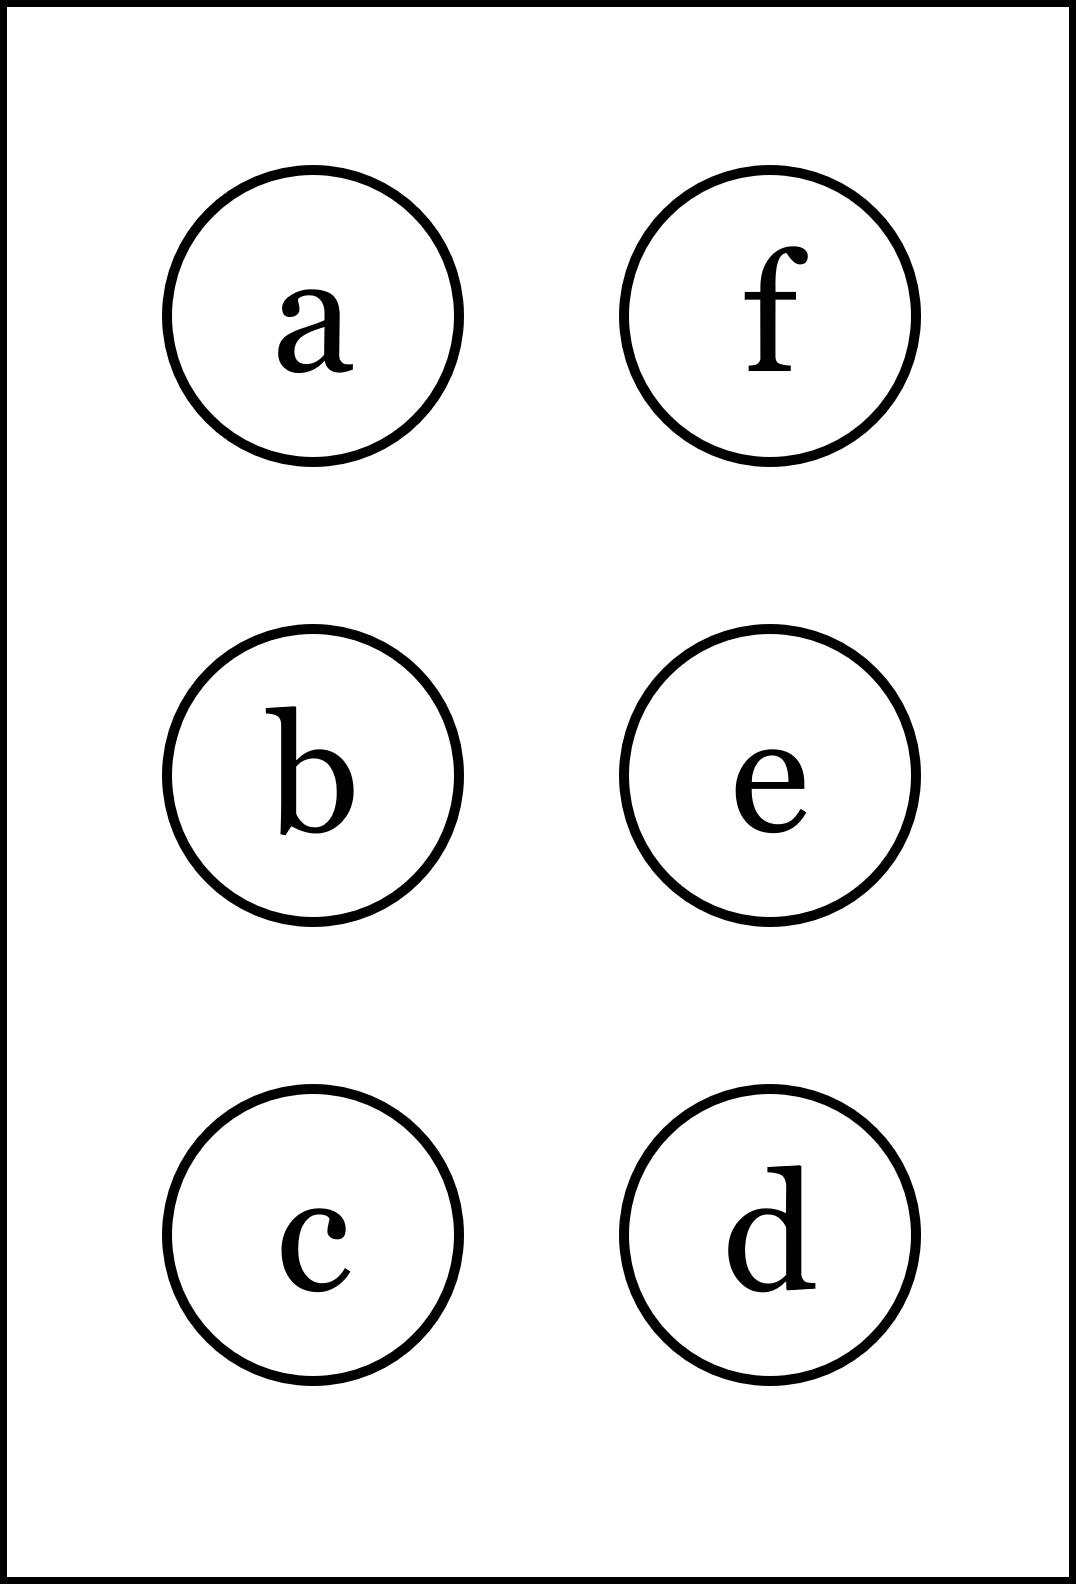
\includegraphics[height=40mm]{../images/braille.png}
{\small Písmeno Braillovej abecedy}
\end{center}
\end{minipage}
\end{center}
\end{minipage}
\\ \hdashline
\begin{minipage}[c][104.5mm][t]{0.5\linewidth}
\begin{center}
\vspace{7mm}
{\huge Limity, skupina \textit{Zeta $\zeta$} -\romannumeral3}\\[5mm]
\textit{Meno:}\phantom{xxxxxxxxxxxxxxxxxxxxxxxxxxxxxxxxxxxxxxxxxxxxxxxxxxxxxxxxxxxxxxxxx}\\[5mm]
\begin{minipage}{0.95\linewidth}
\begin{center}
\textbf{Vypočti limity}. Pokud se výsledky shodujú s tými za otazníky, tak napravo\\obarvi příslušející kroužek načerno. \textbf{Spolu odevzdejte výsledné slovo}.
\end{center}
\end{minipage}
\\[1mm]
\begin{minipage}{0.79\linewidth}
\begin{center}
\begin{varwidth}{\linewidth}
\begin{enumerate}
\normalsize
\item $\lim\limits_{n\to\infty}\cfrac{4+2n}{-3-n}$\quad \dotfill\; ???\;\dotfill \quad $-2$
\item $\lim\limits_{n\to\infty}\cfrac{-4(2-6n)}{(2n-5)^2}$\quad \dotfill\; ???\;\dotfill \quad $0$
\item $\lim\limits_{n\to\infty}\cfrac{(-5+2n)^2}{n^2-8n+2}$\quad \dotfill\; ???\;\dotfill \quad $4$
\item $\lim\limits_{n\to\infty}\cfrac{2^{n-2}}{2^{n-3}}$\quad \dotfill\; ???\;\dotfill \quad $-\infty$
\item $\lim\limits_{n\to\infty}\cfrac{\left(\frac{3}{2}\right)^n -2}{-4n^{-4}}$\quad \dotfill\; ???\;\dotfill \quad $-\infty$
\item $\lim\limits_{n\to\infty}\cfrac{-2\cdot 2^{n+2}+2\cdot 3^{n-2}}{-9\cdot 3^{n+1}+6\cdot 2^{n-2}}$\quad \dotfill\; ???\;\dotfill \quad $\nicefrac{-2}{3}$
\end{enumerate}
\end{varwidth}
\end{center}
\end{minipage}
\begin{minipage}{0.20\linewidth}
\begin{center}
{\Huge\bfseries 3.} \\[2mm]
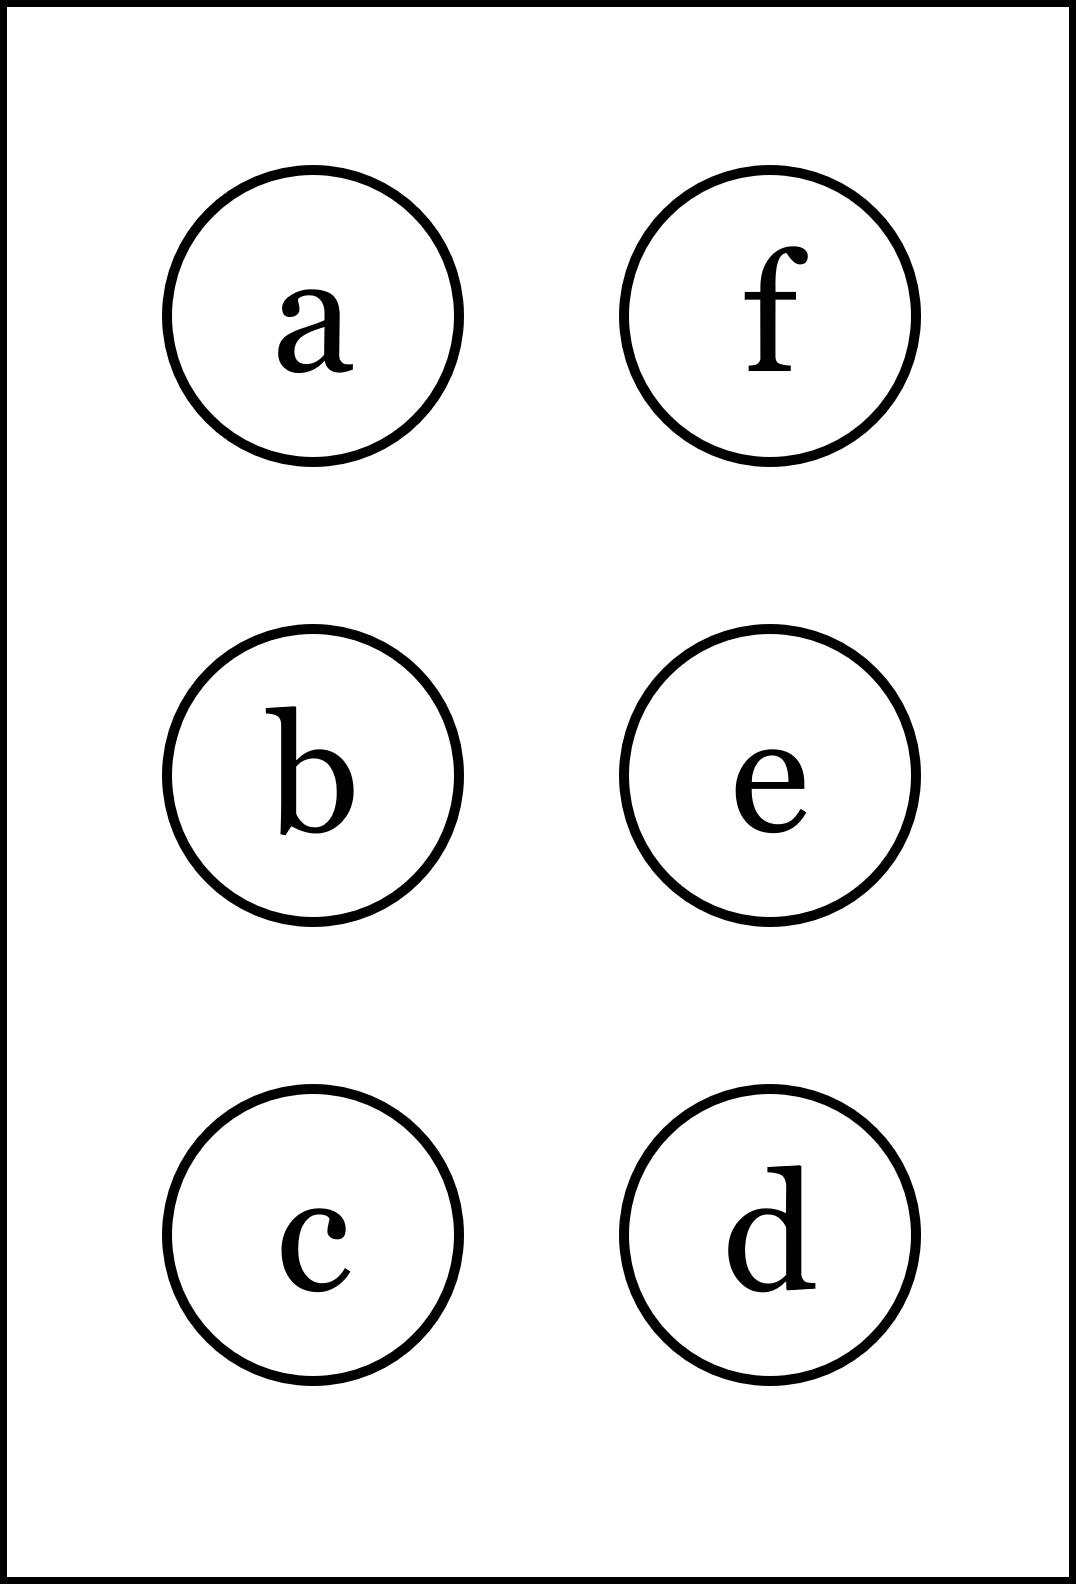
\includegraphics[height=40mm]{../images/braille.png}
{\small Písmeno Braillovej abecedy}
\end{center}
\end{minipage}
\end{center}
\end{minipage}
&
\begin{minipage}[c][104.5mm][t]{0.5\linewidth}
\begin{center}
\vspace{7mm}
{\huge Limity, skupina \textit{Zeta $\zeta$} -\romannumeral4}\\[5mm]
\textit{Meno:}\phantom{xxxxxxxxxxxxxxxxxxxxxxxxxxxxxxxxxxxxxxxxxxxxxxxxxxxxxxxxxxxxxxxxx}\\[5mm]
\begin{minipage}{0.95\linewidth}
\begin{center}
\textbf{Vypočti limity}. Pokud se výsledky shodujú s tými za otazníky, tak napravo\\obarvi příslušející kroužek načerno. \textbf{Spolu odevzdejte výsledné slovo}.
\end{center}
\end{minipage}
\\[1mm]
\begin{minipage}{0.79\linewidth}
\begin{center}
\begin{varwidth}{\linewidth}
\begin{enumerate}
\normalsize
\item $\lim\limits_{n\to\infty}\cfrac{-7-3n}{-5-2n}$\quad \dotfill\; ???\;\dotfill \quad $\nicefrac{3}{2}$
\item $\lim\limits_{n\to\infty}\cfrac{-3(-5-6n)}{(n+2)^2}$\quad \dotfill\; ???\;\dotfill \quad $-\infty$
\item $\lim\limits_{n\to\infty}\cfrac{(5+2n)^2}{n^2+4n+4}$\quad \dotfill\; ???\;\dotfill \quad $4$
\item $\lim\limits_{n\to\infty}\cfrac{4^{n+4}}{4^{n+3}}$\quad \dotfill\; ???\;\dotfill \quad $256$
\item $\lim\limits_{n\to\infty}\cfrac{\left(\frac{2}{3}\right)^n -1}{-4n^{-8}}$\quad \dotfill\; ???\;\dotfill \quad $\infty$
\item $\lim\limits_{n\to\infty}\cfrac{8\cdot 2^{n-2}-2\cdot 4^{n+1}}{4\cdot 4^{n+1}-2\cdot 2^{n-1}}$\quad \dotfill\; ???\;\dotfill \quad $\nicefrac{-1}{4}$
\end{enumerate}
\end{varwidth}
\end{center}
\end{minipage}
\begin{minipage}{0.20\linewidth}
\begin{center}
{\Huge\bfseries 4.} \\[2mm]
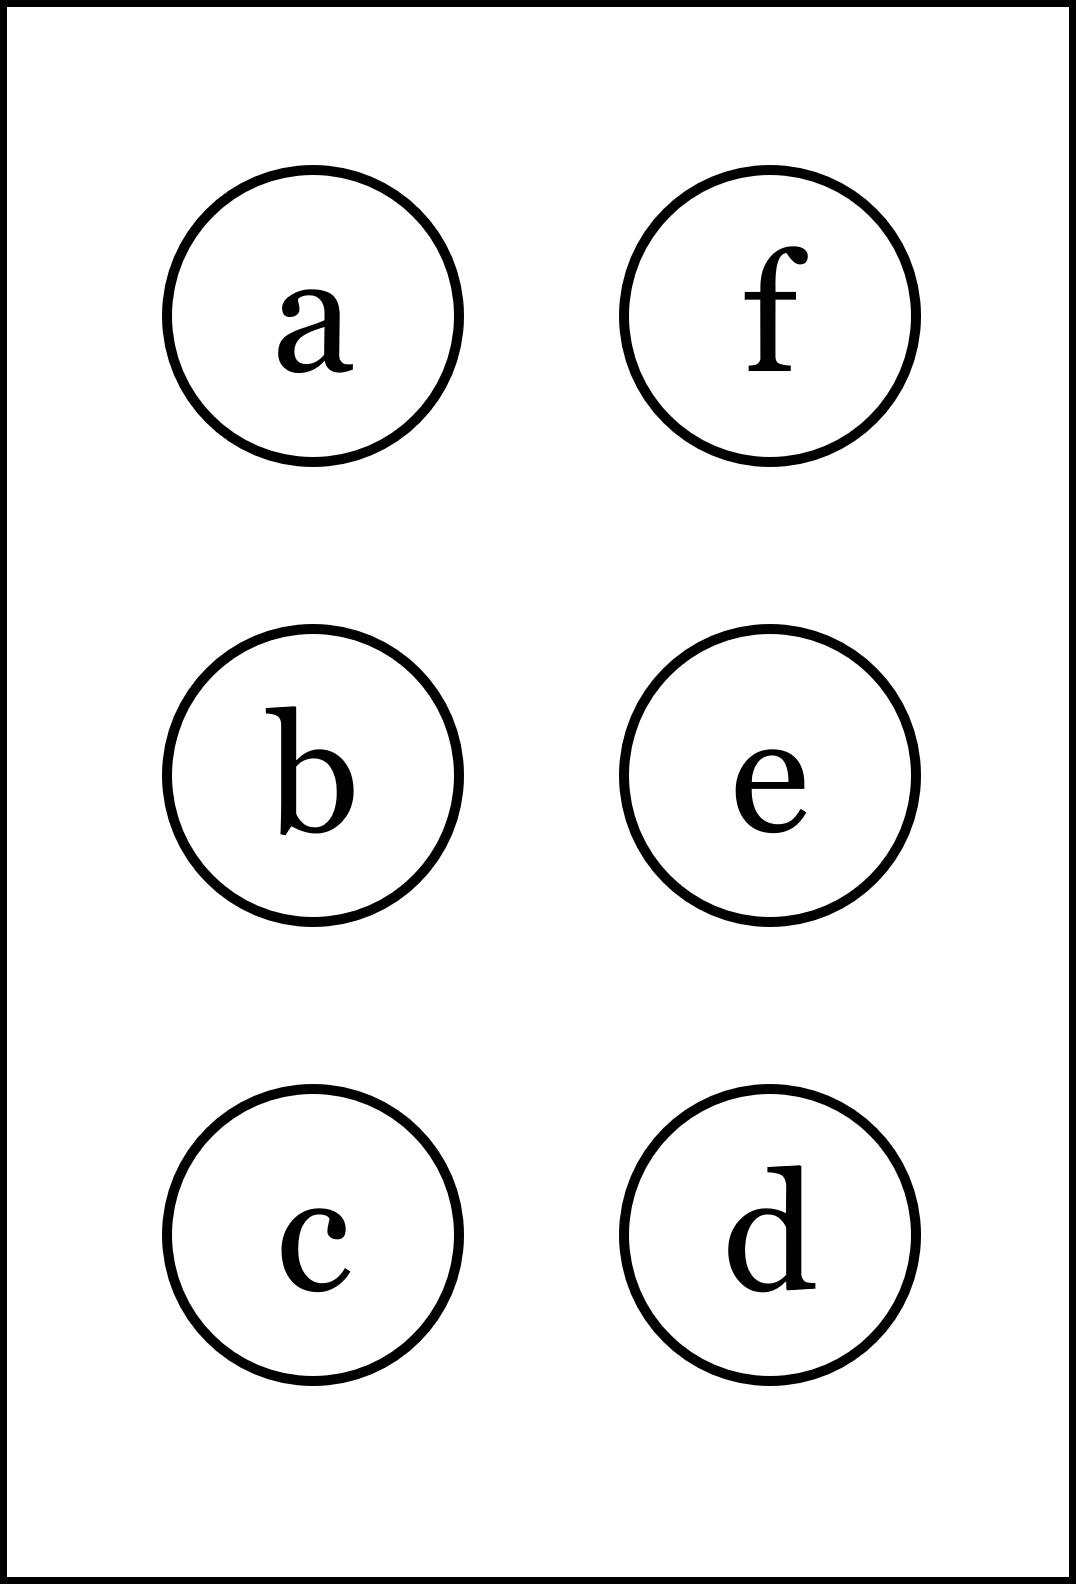
\includegraphics[height=40mm]{../images/braille.png}
{\small Písmeno Braillovej abecedy}
\end{center}
\end{minipage}
\end{center}
\end{minipage}
%
\end{tabular}
\newpage
\thispagestyle{empty}
\begin{tabular}{c:c}
\begin{minipage}[c][104.5mm][t]{0.5\linewidth}
\begin{center}
\vspace{7mm}
{\huge Limity, skupina \textit{Eta $\eta$} -\romannumeral1}\\[5mm]
\textit{Meno:}\phantom{xxxxxxxxxxxxxxxxxxxxxxxxxxxxxxxxxxxxxxxxxxxxxxxxxxxxxxxxxxxxxxxxx}\\[5mm]
\begin{minipage}{0.95\linewidth}
\begin{center}
\textbf{Vypočti limity}. Pokud se výsledky shodujú s tými za otazníky, tak napravo\\obarvi příslušející kroužek načerno. \textbf{Spolu odevzdejte výsledné slovo}.
\end{center}
\end{minipage}
\\[1mm]
\begin{minipage}{0.79\linewidth}
\begin{center}
\begin{varwidth}{\linewidth}
\begin{enumerate}
\normalsize
\item $\lim\limits_{n\to\infty}\cfrac{4+3n}{-3-n}$\quad \dotfill\; ???\;\dotfill \quad $0$
\item $\lim\limits_{n\to\infty}\cfrac{2(-5+4n)}{(-6n+6)^2}$\quad \dotfill\; ???\;\dotfill \quad $0$
\item $\lim\limits_{n\to\infty}\cfrac{(4-3n)^2}{n^2-2n-3}$\quad \dotfill\; ???\;\dotfill \quad $-\infty$
\item $\lim\limits_{n\to\infty}\cfrac{4^{n+2}}{4^{n+1}}$\quad \dotfill\; ???\;\dotfill \quad $-\infty$
\item $\lim\limits_{n\to\infty}\cfrac{\left(\frac{3}{4}\right)^n -3}{n^{-8}}$\quad \dotfill\; ???\;\dotfill \quad $-\infty$
\item $\lim\limits_{n\to\infty}\cfrac{4\cdot 2^{n+2}+6\cdot 3^{n-2}}{4\cdot 3^{n-1}+6\cdot 2^{n-1}}$\quad \dotfill\; ???\;\dotfill \quad $\nicefrac{1}{2}$
\end{enumerate}
\end{varwidth}
\end{center}
\end{minipage}
\begin{minipage}{0.20\linewidth}
\begin{center}
{\Huge\bfseries 1.} \\[2mm]
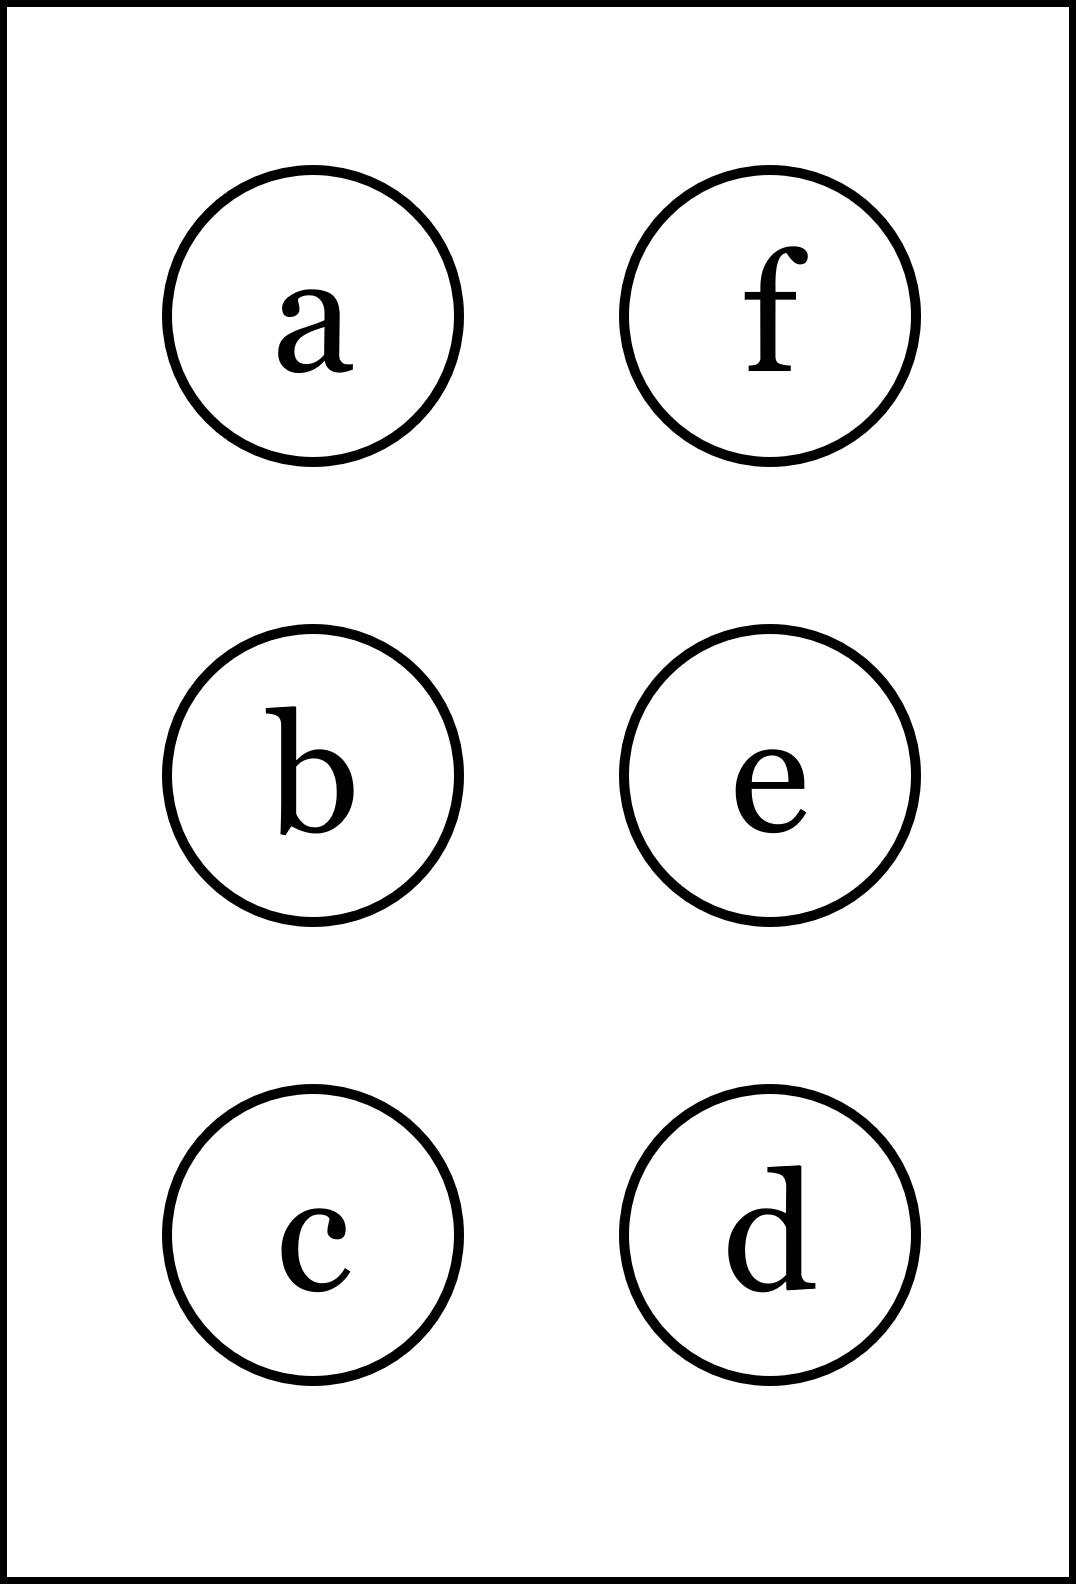
\includegraphics[height=40mm]{../images/braille.png}
{\small Písmeno Braillovej abecedy}
\end{center}
\end{minipage}
\end{center}
\end{minipage}
&
\begin{minipage}[c][104.5mm][t]{0.5\linewidth}
\begin{center}
\vspace{7mm}
{\huge Limity, skupina \textit{Eta $\eta$} -\romannumeral2}\\[5mm]
\textit{Meno:}\phantom{xxxxxxxxxxxxxxxxxxxxxxxxxxxxxxxxxxxxxxxxxxxxxxxxxxxxxxxxxxxxxxxxx}\\[5mm]
\begin{minipage}{0.95\linewidth}
\begin{center}
\textbf{Vypočti limity}. Pokud se výsledky shodujú s tými za otazníky, tak napravo\\obarvi příslušející kroužek načerno. \textbf{Spolu odevzdejte výsledné slovo}.
\end{center}
\end{minipage}
\\[1mm]
\begin{minipage}{0.79\linewidth}
\begin{center}
\begin{varwidth}{\linewidth}
\begin{enumerate}
\normalsize
\item $\lim\limits_{n\to\infty}\cfrac{6+7n}{2-5n}$\quad \dotfill\; ???\;\dotfill \quad $\nicefrac{-7}{5}$
\item $\lim\limits_{n\to\infty}\cfrac{-3(-6-8n)}{(-3n+6)^2}$\quad \dotfill\; ???\;\dotfill \quad $-\infty$
\item $\lim\limits_{n\to\infty}\cfrac{(5+n)^2}{n^2+3n+1}$\quad \dotfill\; ???\;\dotfill \quad $0$
\item $\lim\limits_{n\to\infty}\cfrac{3^{n-2}}{3^{n-3}}$\quad \dotfill\; ???\;\dotfill \quad $0$
\item $\lim\limits_{n\to\infty}\cfrac{\left(\frac{3}{2}\right)^n -2}{-2n^{-4}}$\quad \dotfill\; ???\;\dotfill \quad $0$
\item $\lim\limits_{n\to\infty}\cfrac{-4\cdot 2^{n+1}-4\cdot 4^{n+2}}{8\cdot 4^{n-2}+4\cdot 2^{n+2}}$\quad \dotfill\; ???\;\dotfill \quad $\nicefrac{-1}{8}$
\end{enumerate}
\end{varwidth}
\end{center}
\end{minipage}
\begin{minipage}{0.20\linewidth}
\begin{center}
{\Huge\bfseries 2.} \\[2mm]
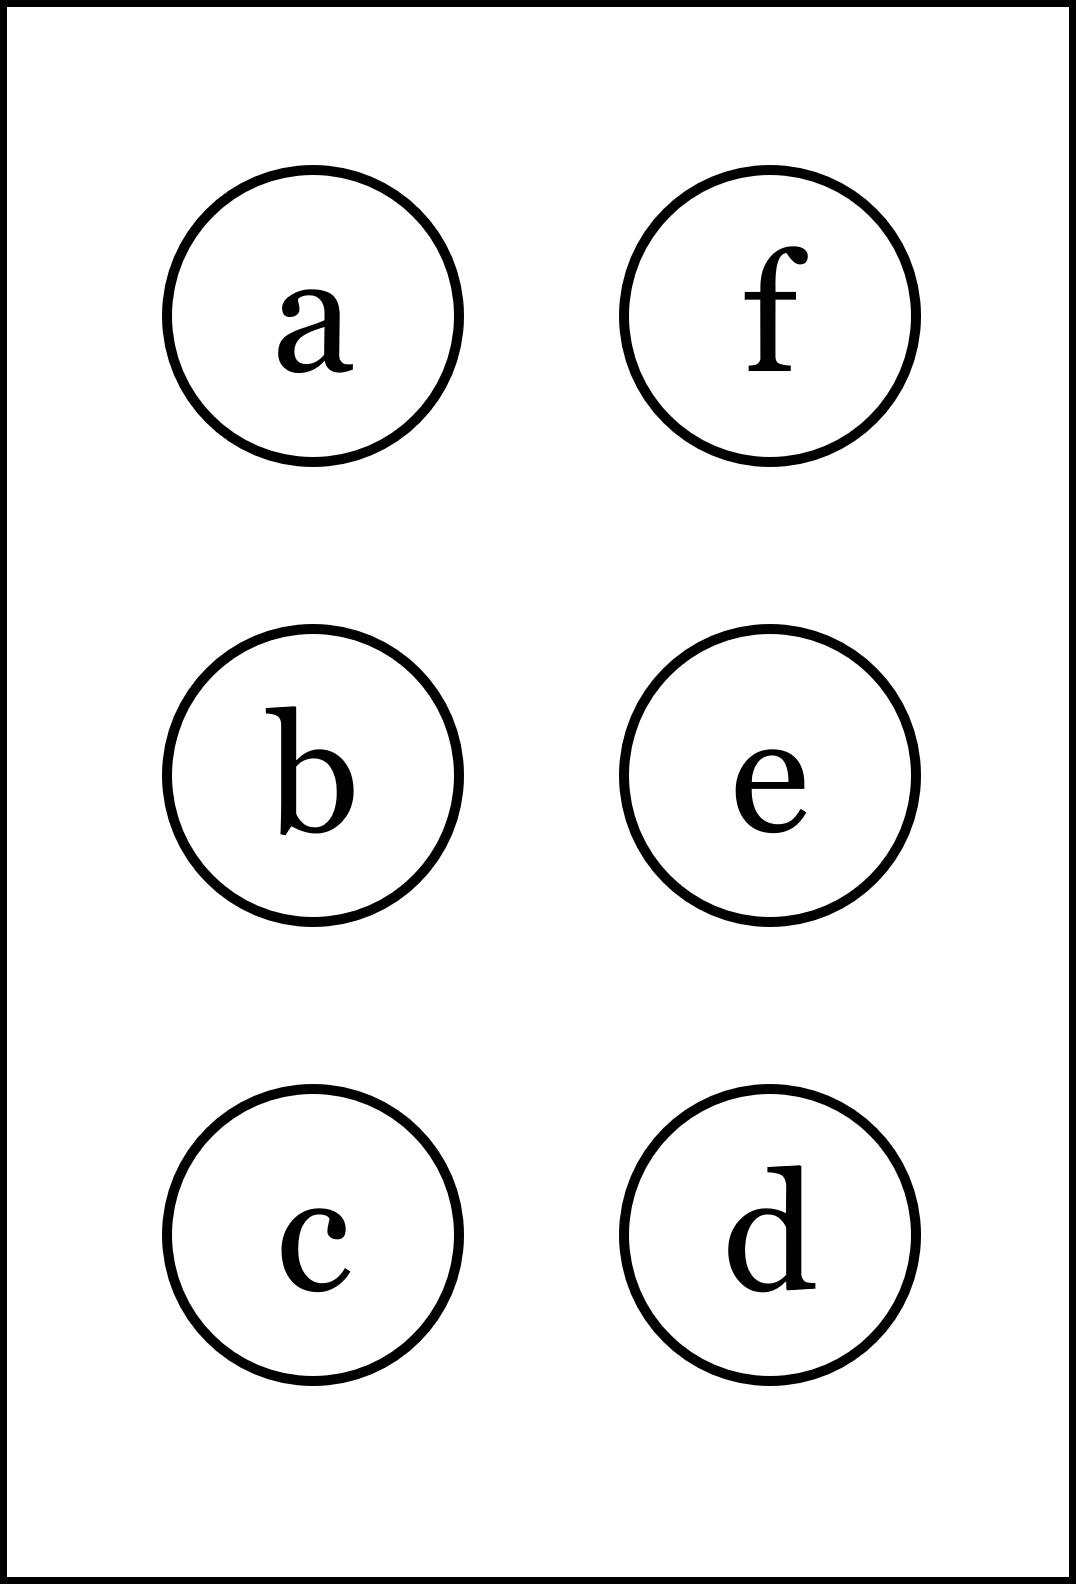
\includegraphics[height=40mm]{../images/braille.png}
{\small Písmeno Braillovej abecedy}
\end{center}
\end{minipage}
\end{center}
\end{minipage}
\\ \hdashline
\begin{minipage}[c][104.5mm][t]{0.5\linewidth}
\begin{center}
\vspace{7mm}
{\huge Limity, skupina \textit{Eta $\eta$} -\romannumeral3}\\[5mm]
\textit{Meno:}\phantom{xxxxxxxxxxxxxxxxxxxxxxxxxxxxxxxxxxxxxxxxxxxxxxxxxxxxxxxxxxxxxxxxx}\\[5mm]
\begin{minipage}{0.95\linewidth}
\begin{center}
\textbf{Vypočti limity}. Pokud se výsledky shodujú s tými za otazníky, tak napravo\\obarvi příslušející kroužek načerno. \textbf{Spolu odevzdejte výsledné slovo}.
\end{center}
\end{minipage}
\\[1mm]
\begin{minipage}{0.79\linewidth}
\begin{center}
\begin{varwidth}{\linewidth}
\begin{enumerate}
\normalsize
\item $\lim\limits_{n\to\infty}\cfrac{-7-2n}{5+4n}$\quad \dotfill\; ???\;\dotfill \quad $\nicefrac{-1}{2}$
\item $\lim\limits_{n\to\infty}\cfrac{-5(-8-2n)}{(-5n-5)^2}$\quad \dotfill\; ???\;\dotfill \quad $-\infty$
\item $\lim\limits_{n\to\infty}\cfrac{(-9+6n)^2}{n^2+5n-3}$\quad \dotfill\; ???\;\dotfill \quad $36$
\item $\lim\limits_{n\to\infty}\cfrac{2^{n+1}}{2^{n-1}}$\quad \dotfill\; ???\;\dotfill \quad $2$
\item $\lim\limits_{n\to\infty}\cfrac{\left(\frac{2}{4}\right)^n +4}{2n^{-9}}$\quad \dotfill\; ???\;\dotfill \quad $\infty$
\item $\lim\limits_{n\to\infty}\cfrac{-4\cdot 3^{n+2}+12\cdot 4^{n-1}}{-12\cdot 4^{n-1}-4\cdot 3^{n-2}}$\quad \dotfill\; ???\;\dotfill \quad $-1$
\end{enumerate}
\end{varwidth}
\end{center}
\end{minipage}
\begin{minipage}{0.20\linewidth}
\begin{center}
{\Huge\bfseries 3.} \\[2mm]
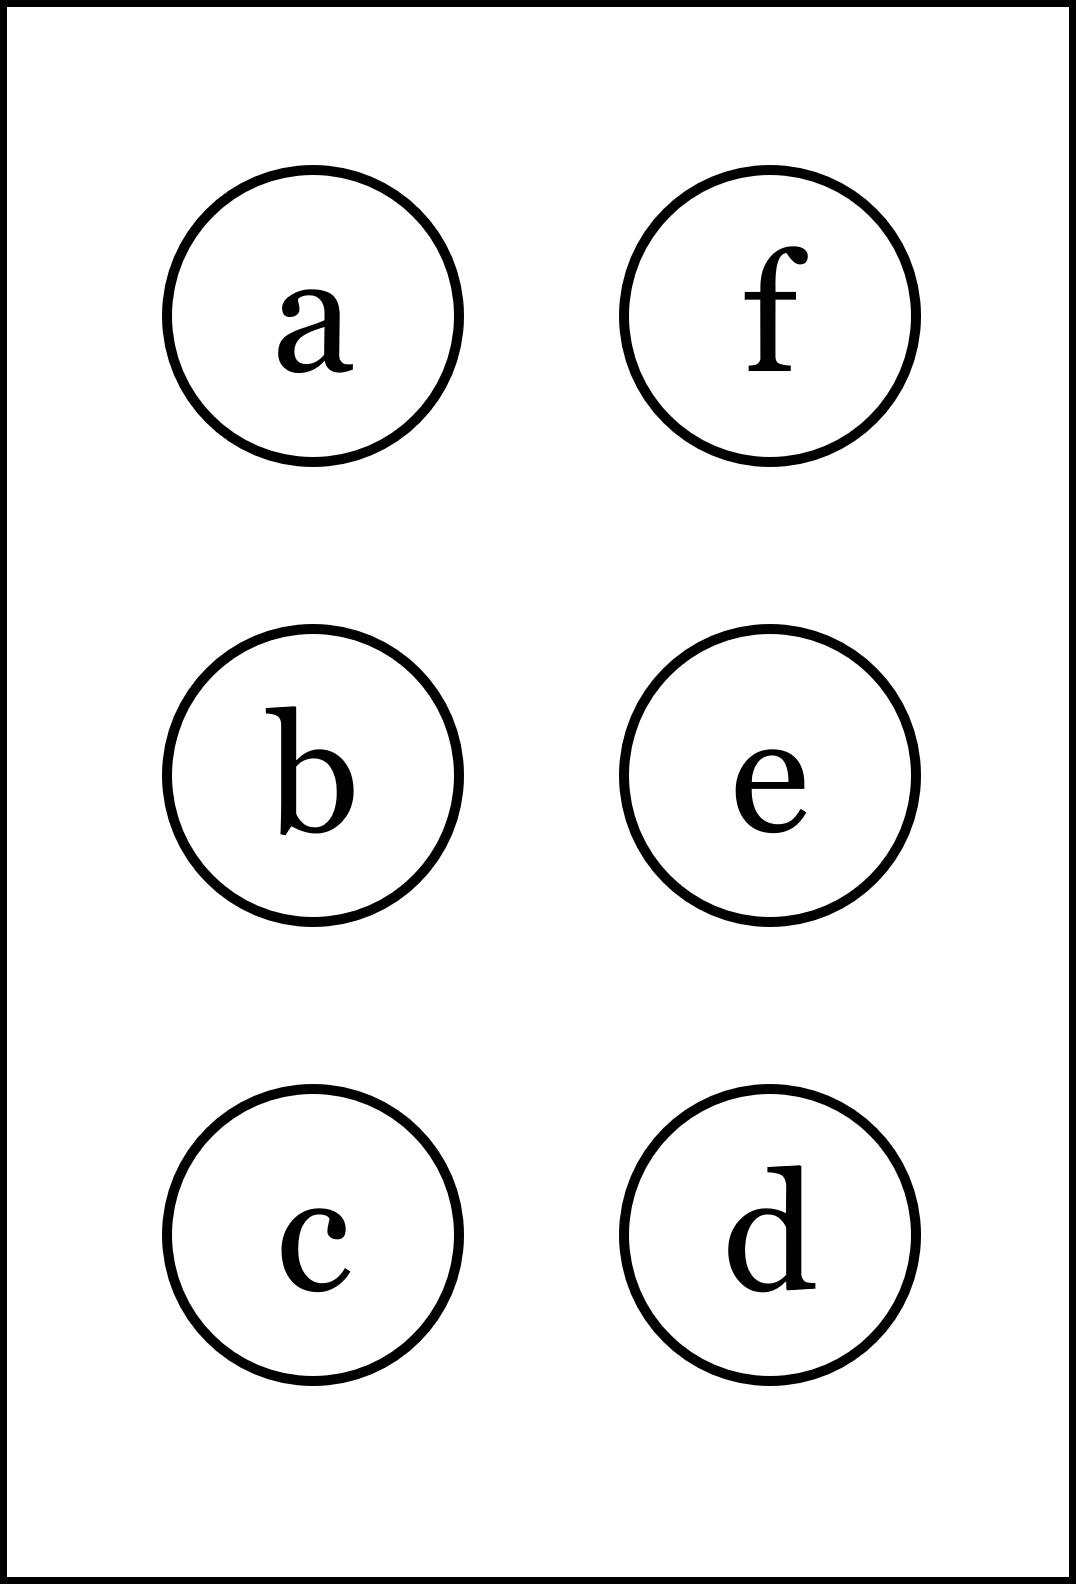
\includegraphics[height=40mm]{../images/braille.png}
{\small Písmeno Braillovej abecedy}
\end{center}
\end{minipage}
\end{center}
\end{minipage}
&
\begin{minipage}[c][104.5mm][t]{0.5\linewidth}
\begin{center}
\vspace{7mm}
{\huge Limity, skupina \textit{Eta $\eta$} -\romannumeral4}\\[5mm]
\textit{Meno:}\phantom{xxxxxxxxxxxxxxxxxxxxxxxxxxxxxxxxxxxxxxxxxxxxxxxxxxxxxxxxxxxxxxxxx}\\[5mm]
\begin{minipage}{0.95\linewidth}
\begin{center}
\textbf{Vypočti limity}. Pokud se výsledky shodujú s tými za otazníky, tak napravo\\obarvi příslušející kroužek načerno. \textbf{Spolu odevzdejte výsledné slovo}.
\end{center}
\end{minipage}
\\[1mm]
\begin{minipage}{0.79\linewidth}
\begin{center}
\begin{varwidth}{\linewidth}
\begin{enumerate}
\normalsize
\item $\lim\limits_{n\to\infty}\cfrac{4+2n}{-1+3n}$\quad \dotfill\; ???\;\dotfill \quad $\nicefrac{2}{3}$
\item $\lim\limits_{n\to\infty}\cfrac{-3(-3-2n)}{(5n-5)^2}$\quad \dotfill\; ???\;\dotfill \quad $\infty$
\item $\lim\limits_{n\to\infty}\cfrac{(3+4n)^2}{n^2+2n-4}$\quad \dotfill\; ???\;\dotfill \quad $\nicefrac{-3}{4}$
\item $\lim\limits_{n\to\infty}\cfrac{3^{n+2}}{3^{n+2}}$\quad \dotfill\; ???\;\dotfill \quad $\infty$
\item $\lim\limits_{n\to\infty}\cfrac{\left(\frac{2}{4}\right)^n +1}{2n^{-4}}$\quad \dotfill\; ???\;\dotfill \quad $0$
\item $\lim\limits_{n\to\infty}\cfrac{6\cdot 2^{n+1}-9\cdot 3^{n+2}}{2\cdot 3^{n-2}+2\cdot 2^{n+2}}$\quad \dotfill\; ???\;\dotfill \quad $\nicefrac{-3}{2}$
\end{enumerate}
\end{varwidth}
\end{center}
\end{minipage}
\begin{minipage}{0.20\linewidth}
\begin{center}
{\Huge\bfseries 4.} \\[2mm]
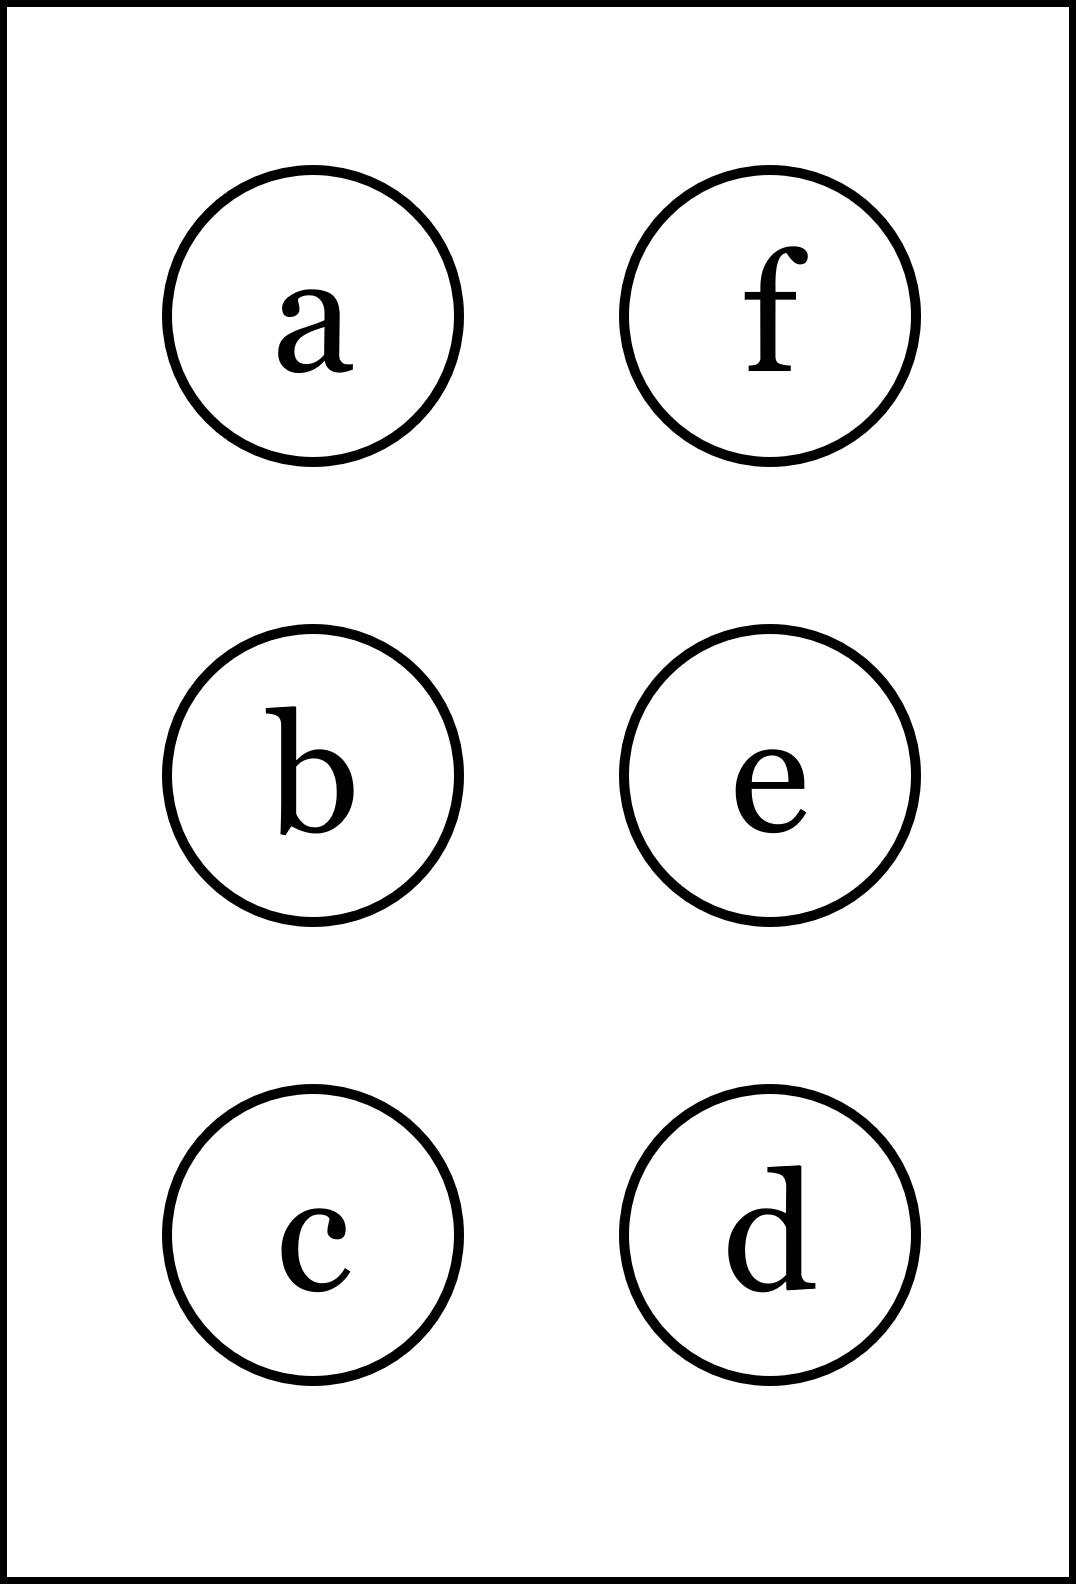
\includegraphics[height=40mm]{../images/braille.png}
{\small Písmeno Braillovej abecedy}
\end{center}
\end{minipage}
\end{center}
\end{minipage}
%
\end{tabular}
\newpage
\thispagestyle{empty}
\begin{tabular}{c:c}
\begin{minipage}[c][104.5mm][t]{0.5\linewidth}
\begin{center}
\vspace{7mm}
{\huge Limity, skupina \textit{Theta $\theta$} -\romannumeral1}\\[5mm]
\textit{Meno:}\phantom{xxxxxxxxxxxxxxxxxxxxxxxxxxxxxxxxxxxxxxxxxxxxxxxxxxxxxxxxxxxxxxxxx}\\[5mm]
\begin{minipage}{0.95\linewidth}
\begin{center}
\textbf{Vypočti limity}. Pokud se výsledky shodujú s tými za otazníky, tak napravo\\obarvi příslušející kroužek načerno. \textbf{Spolu odevzdejte výsledné slovo}.
\end{center}
\end{minipage}
\\[1mm]
\begin{minipage}{0.79\linewidth}
\begin{center}
\begin{varwidth}{\linewidth}
\begin{enumerate}
\normalsize
\item $\lim\limits_{n\to\infty}\cfrac{-4+2n}{-5-2n}$\quad \dotfill\; ???\;\dotfill \quad $-1$
\item $\lim\limits_{n\to\infty}\cfrac{7(-7-n)}{(4n+1)^2}$\quad \dotfill\; ???\;\dotfill \quad $0$
\item $\lim\limits_{n\to\infty}\cfrac{(-3-3n)^2}{n^2+8n+6}$\quad \dotfill\; ???\;\dotfill \quad $9$
\item $\lim\limits_{n\to\infty}\cfrac{3^{n-1}}{3^{n+2}}$\quad \dotfill\; ???\;\dotfill \quad $0$
\item $\lim\limits_{n\to\infty}\cfrac{\left(\frac{1}{3}\right)^n -2}{3n^{6}}$\quad \dotfill\; ???\;\dotfill \quad $0$
\item $\lim\limits_{n\to\infty}\cfrac{4\cdot 2^{n-2}-16\cdot 4^{n-1}}{-16\cdot 4^{n+2}+16\cdot 2^{n-2}}$\quad \dotfill\; ???\;\dotfill \quad $4$
\end{enumerate}
\end{varwidth}
\end{center}
\end{minipage}
\begin{minipage}{0.20\linewidth}
\begin{center}
{\Huge\bfseries 1.} \\[2mm]
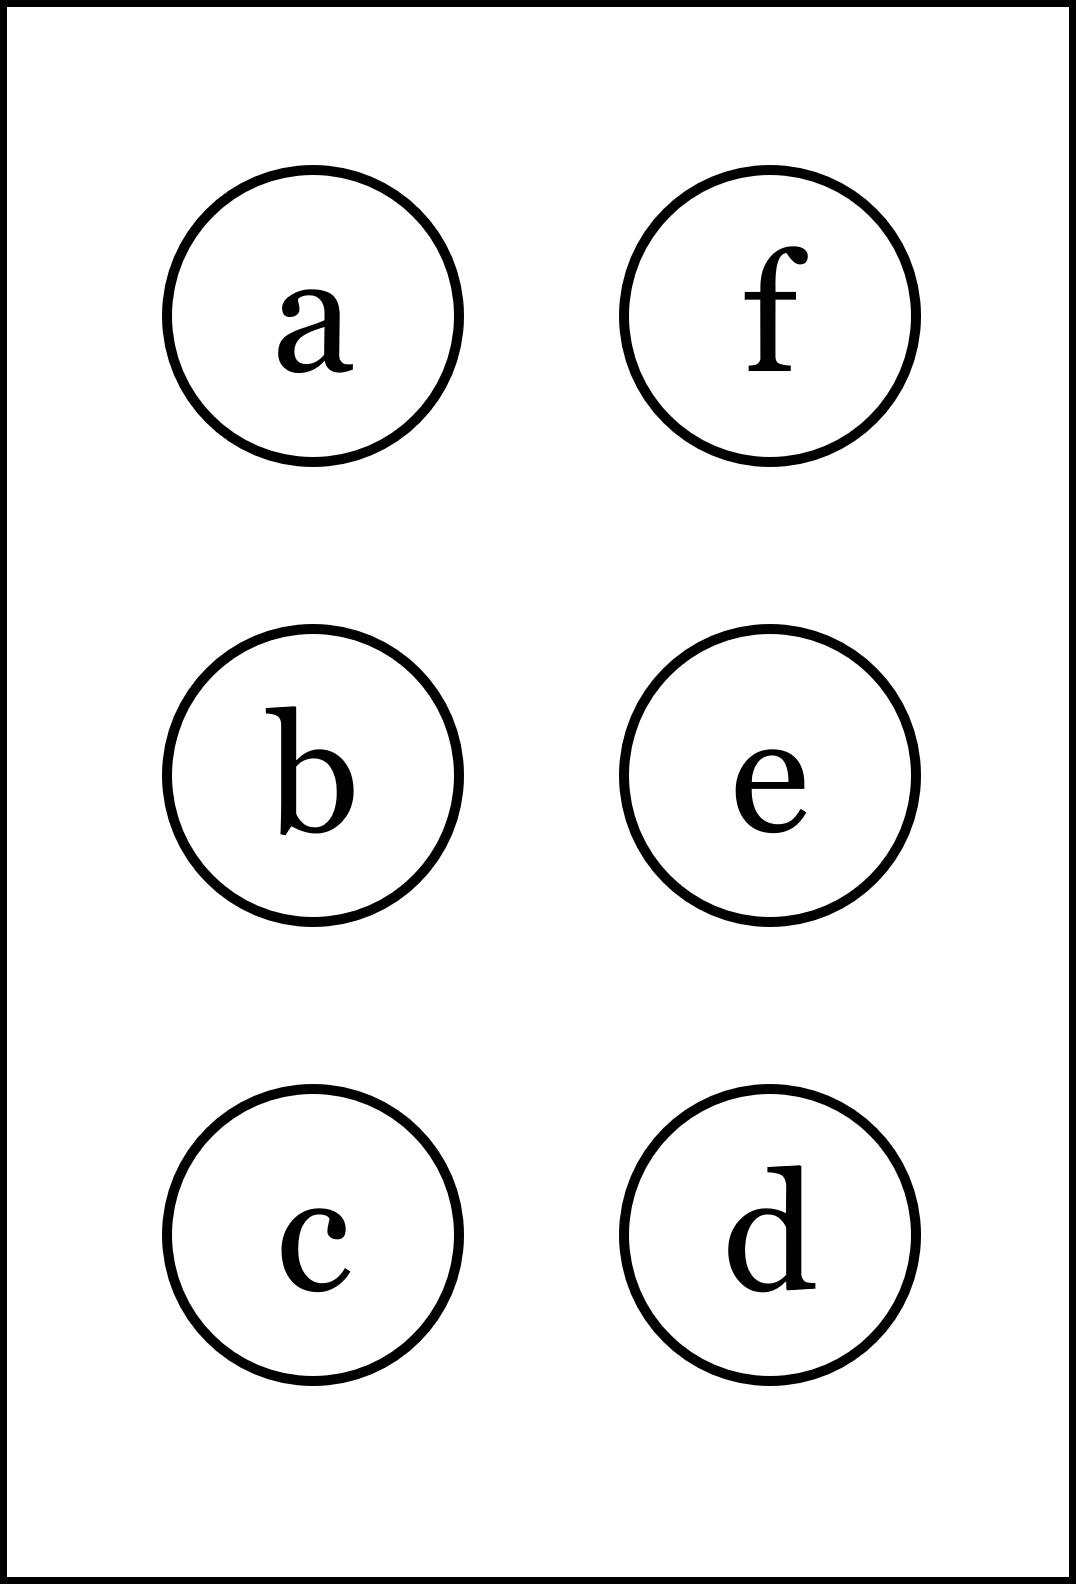
\includegraphics[height=40mm]{../images/braille.png}
{\small Písmeno Braillovej abecedy}
\end{center}
\end{minipage}
\end{center}
\end{minipage}
&
\begin{minipage}[c][104.5mm][t]{0.5\linewidth}
\begin{center}
\vspace{7mm}
{\huge Limity, skupina \textit{Theta $\theta$} -\romannumeral2}\\[5mm]
\textit{Meno:}\phantom{xxxxxxxxxxxxxxxxxxxxxxxxxxxxxxxxxxxxxxxxxxxxxxxxxxxxxxxxxxxxxxxxx}\\[5mm]
\begin{minipage}{0.95\linewidth}
\begin{center}
\textbf{Vypočti limity}. Pokud se výsledky shodujú s tými za otazníky, tak napravo\\obarvi příslušející kroužek načerno. \textbf{Spolu odevzdejte výsledné slovo}.
\end{center}
\end{minipage}
\\[1mm]
\begin{minipage}{0.79\linewidth}
\begin{center}
\begin{varwidth}{\linewidth}
\begin{enumerate}
\normalsize
\item $\lim\limits_{n\to\infty}\cfrac{1+7n}{-6-n}$\quad \dotfill\; ???\;\dotfill \quad $-7$
\item $\lim\limits_{n\to\infty}\cfrac{-4(8+4n)}{(n+9)^2}$\quad \dotfill\; ???\;\dotfill \quad $\infty$
\item $\lim\limits_{n\to\infty}\cfrac{(6-3n)^2}{n^2-3n-4}$\quad \dotfill\; ???\;\dotfill \quad $-\infty$
\item $\lim\limits_{n\to\infty}\cfrac{2^{n+3}}{2^{n+1}}$\quad \dotfill\; ???\;\dotfill \quad $\nicefrac{1}{4}$
\item $\lim\limits_{n\to\infty}\cfrac{\left(\frac{1}{3}\right)^n -2}{3n^{-4}}$\quad \dotfill\; ???\;\dotfill \quad $\infty$
\item $\lim\limits_{n\to\infty}\cfrac{8\cdot 2^{n+1}-8\cdot 4^{n-2}}{2\cdot 4^{n-1}-2\cdot 2^{n-2}}$\quad \dotfill\; ???\;\dotfill \quad $-16$
\end{enumerate}
\end{varwidth}
\end{center}
\end{minipage}
\begin{minipage}{0.20\linewidth}
\begin{center}
{\Huge\bfseries 2.} \\[2mm]
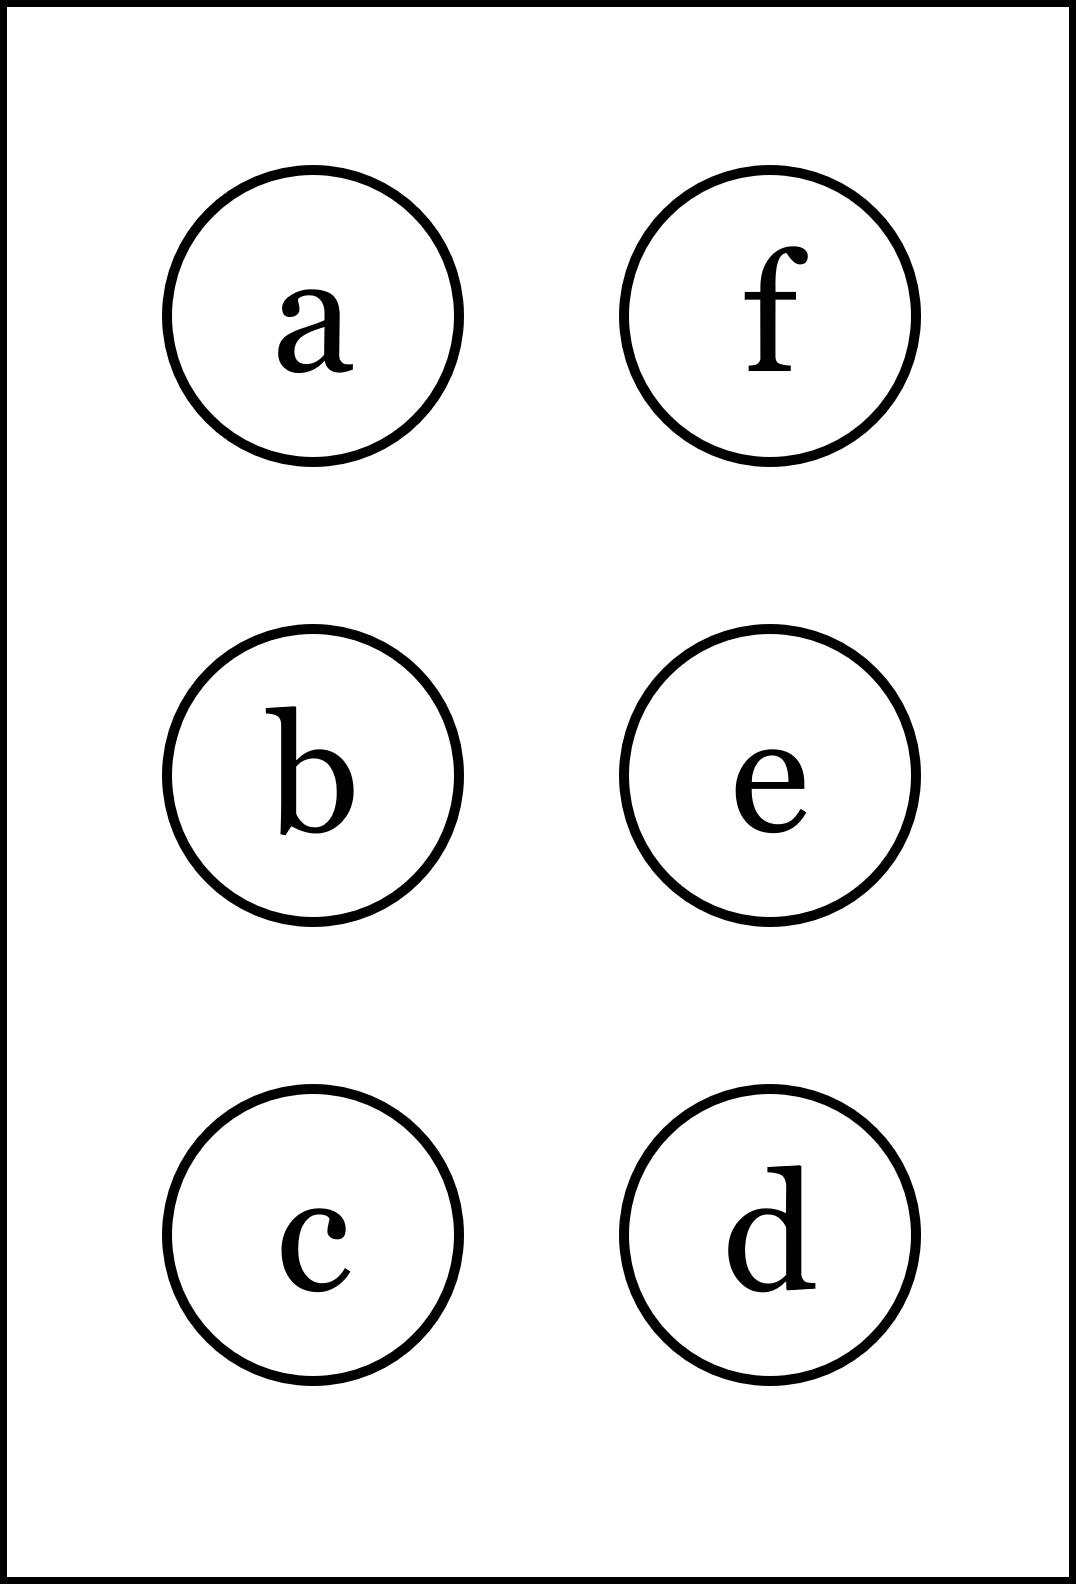
\includegraphics[height=40mm]{../images/braille.png}
{\small Písmeno Braillovej abecedy}
\end{center}
\end{minipage}
\end{center}
\end{minipage}
\\ \hdashline
\begin{minipage}[c][104.5mm][t]{0.5\linewidth}
\begin{center}
\vspace{7mm}
{\huge Limity, skupina \textit{Theta $\theta$} -\romannumeral3}\\[5mm]
\textit{Meno:}\phantom{xxxxxxxxxxxxxxxxxxxxxxxxxxxxxxxxxxxxxxxxxxxxxxxxxxxxxxxxxxxxxxxxx}\\[5mm]
\begin{minipage}{0.95\linewidth}
\begin{center}
\textbf{Vypočti limity}. Pokud se výsledky shodujú s tými za otazníky, tak napravo\\obarvi příslušející kroužek načerno. \textbf{Spolu odevzdejte výsledné slovo}.
\end{center}
\end{minipage}
\\[1mm]
\begin{minipage}{0.79\linewidth}
\begin{center}
\begin{varwidth}{\linewidth}
\begin{enumerate}
\normalsize
\item $\lim\limits_{n\to\infty}\cfrac{5+7n}{-4-4n}$\quad \dotfill\; ???\;\dotfill \quad $\nicefrac{-7}{4}$
\item $\lim\limits_{n\to\infty}\cfrac{1(1+2n)}{(3n-4)^2}$\quad \dotfill\; ???\;\dotfill \quad $\nicefrac{-1}{12}$
\item $\lim\limits_{n\to\infty}\cfrac{(6+3n)^2}{n^2+2n-5}$\quad \dotfill\; ???\;\dotfill \quad $-\infty$
\item $\lim\limits_{n\to\infty}\cfrac{3^{n+2}}{3^{n+1}}$\quad \dotfill\; ???\;\dotfill \quad $\nicefrac{1}{3}$
\item $\lim\limits_{n\to\infty}\cfrac{\left(\frac{1}{4}\right)^n +1}{-n^{-4}}$\quad \dotfill\; ???\;\dotfill \quad $-\infty$
\item $\lim\limits_{n\to\infty}\cfrac{3\cdot 2^{n-2}+9\cdot 3^{n+2}}{-3\cdot 3^{n+1}-2\cdot 2^{n+1}}$\quad \dotfill\; ???\;\dotfill \quad $-9$
\end{enumerate}
\end{varwidth}
\end{center}
\end{minipage}
\begin{minipage}{0.20\linewidth}
\begin{center}
{\Huge\bfseries 3.} \\[2mm]
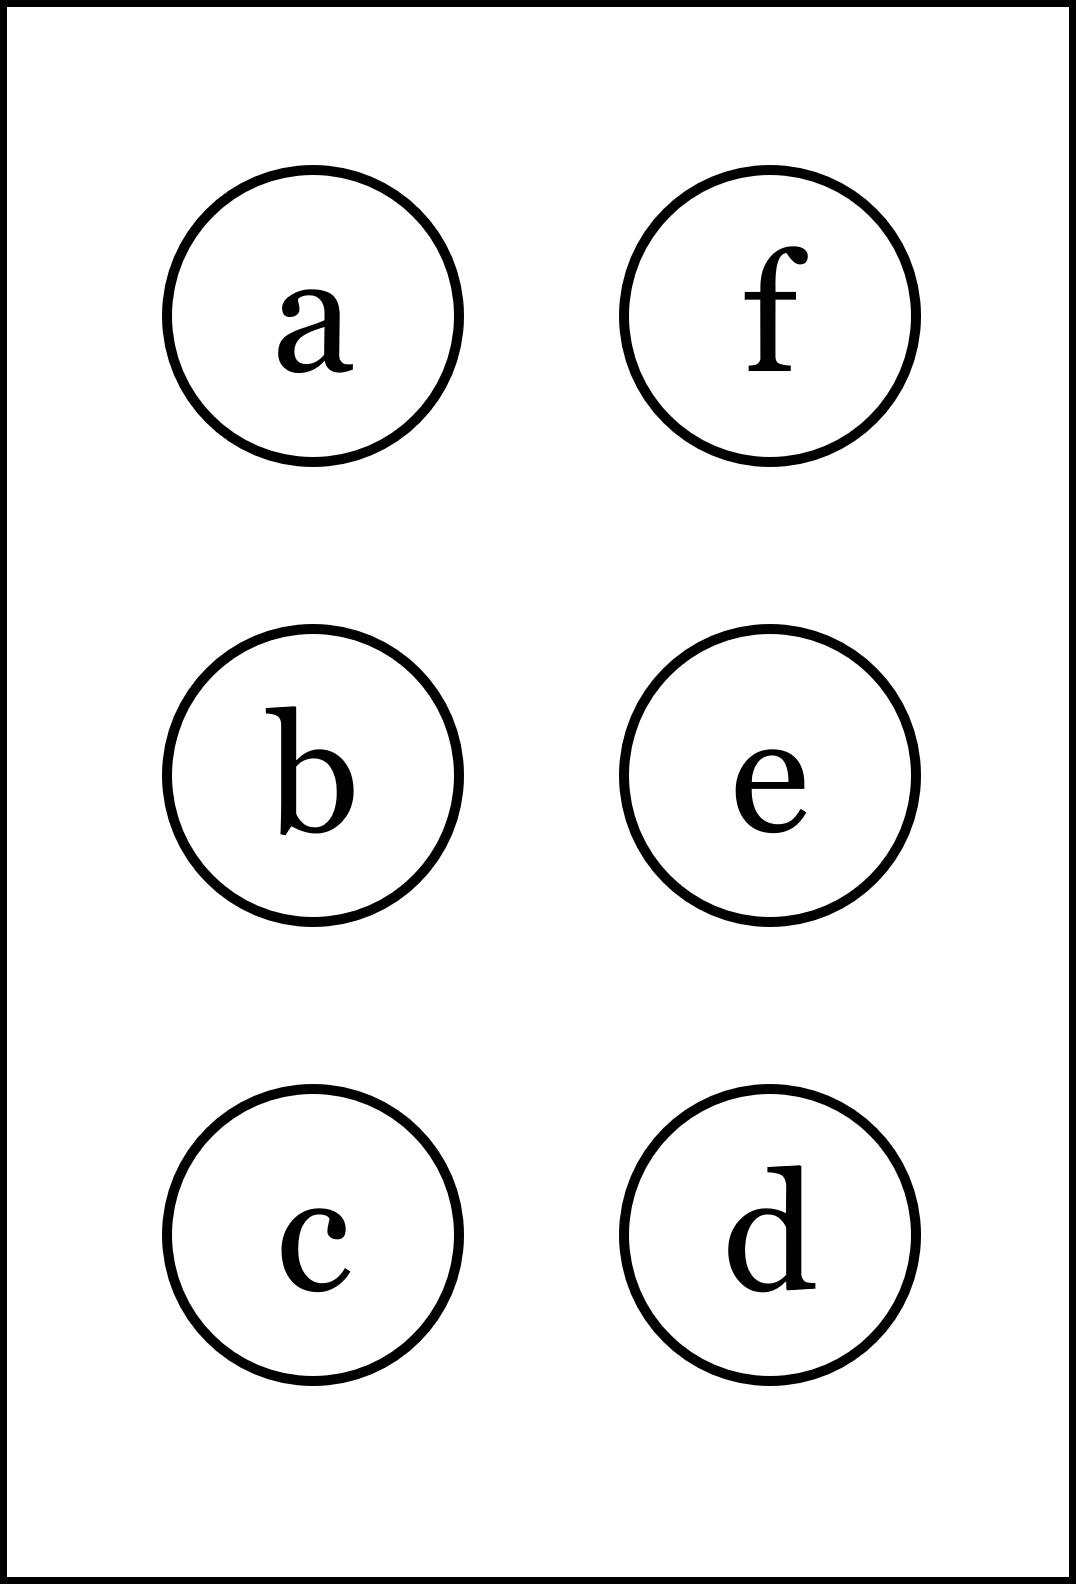
\includegraphics[height=40mm]{../images/braille.png}
{\small Písmeno Braillovej abecedy}
\end{center}
\end{minipage}
\end{center}
\end{minipage}
&
\begin{minipage}[c][104.5mm][t]{0.5\linewidth}
\begin{center}
\vspace{7mm}
{\huge Limity, skupina \textit{Theta $\theta$} -\romannumeral4}\\[5mm]
\textit{Meno:}\phantom{xxxxxxxxxxxxxxxxxxxxxxxxxxxxxxxxxxxxxxxxxxxxxxxxxxxxxxxxxxxxxxxxx}\\[5mm]
\begin{minipage}{0.95\linewidth}
\begin{center}
\textbf{Vypočti limity}. Pokud se výsledky shodujú s tými za otazníky, tak napravo\\obarvi příslušející kroužek načerno. \textbf{Spolu odevzdejte výsledné slovo}.
\end{center}
\end{minipage}
\\[1mm]
\begin{minipage}{0.79\linewidth}
\begin{center}
\begin{varwidth}{\linewidth}
\begin{enumerate}
\normalsize
\item $\lim\limits_{n\to\infty}\cfrac{7-4n}{-2-7n}$\quad \dotfill\; ???\;\dotfill \quad $\nicefrac{4}{7}$
\item $\lim\limits_{n\to\infty}\cfrac{6(1+4n)}{(3n+5)^2}$\quad \dotfill\; ???\;\dotfill \quad $\nicefrac{4}{3}$
\item $\lim\limits_{n\to\infty}\cfrac{(-2+4n)^2}{n^2+6n+7}$\quad \dotfill\; ???\;\dotfill \quad $\infty$
\item $\lim\limits_{n\to\infty}\cfrac{4^{n+2}}{4^{n-2}}$\quad \dotfill\; ???\;\dotfill \quad $-\infty$
\item $\lim\limits_{n\to\infty}\cfrac{\left(\frac{1}{3}\right)^n -2}{-n^{-12}}$\quad \dotfill\; ???\;\dotfill \quad $2$
\item $\lim\limits_{n\to\infty}\cfrac{-6\cdot 2^{n-2}-2\cdot 3^{n-2}}{-9\cdot 3^{n-2}+2\cdot 2^{n-2}}$\quad \dotfill\; ???\;\dotfill \quad $\nicefrac{1}{9}$
\end{enumerate}
\end{varwidth}
\end{center}
\end{minipage}
\begin{minipage}{0.20\linewidth}
\begin{center}
{\Huge\bfseries 4.} \\[2mm]
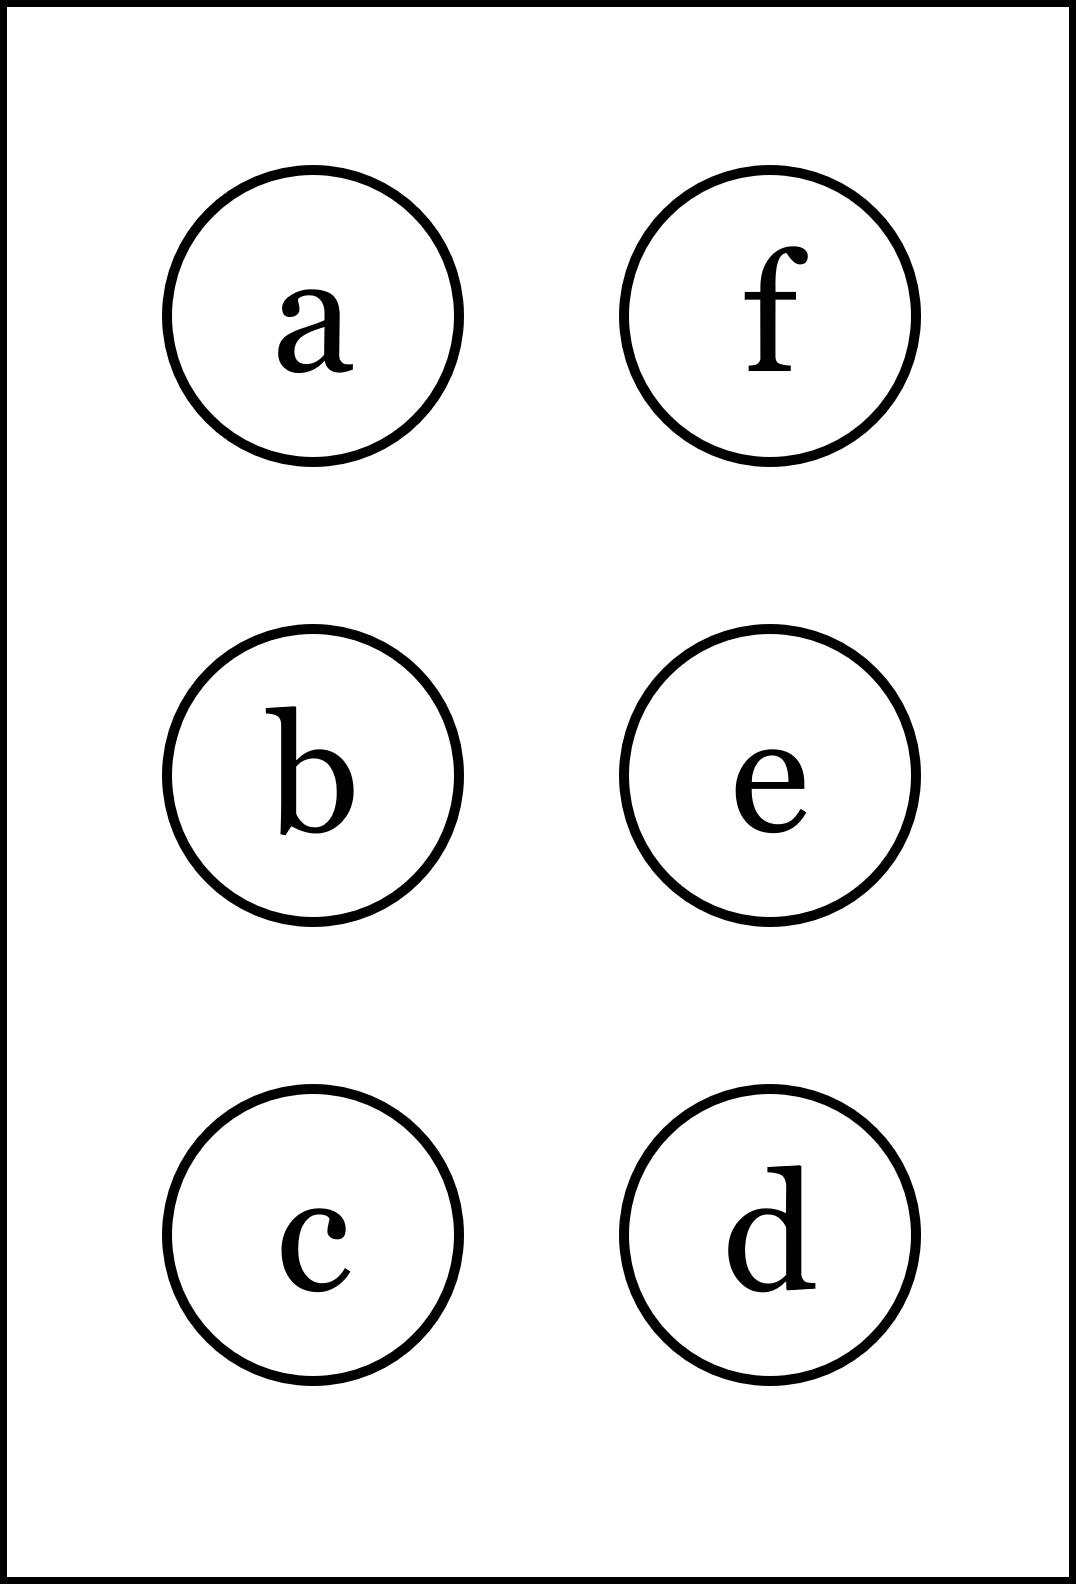
\includegraphics[height=40mm]{../images/braille.png}
{\small Písmeno Braillovej abecedy}
\end{center}
\end{minipage}
\end{center}
\end{minipage}
%
\end{tabular}
\newpage
\thispagestyle{empty}
\begin{tabular}{c:c}
\begin{minipage}[c][104.5mm][t]{0.5\linewidth}
\begin{center}
\vspace{7mm}
{\huge Limity, skupina \textit{Iota $\iota$} -\romannumeral1}\\[5mm]
\textit{Meno:}\phantom{xxxxxxxxxxxxxxxxxxxxxxxxxxxxxxxxxxxxxxxxxxxxxxxxxxxxxxxxxxxxxxxxx}\\[5mm]
\begin{minipage}{0.95\linewidth}
\begin{center}
\textbf{Vypočti limity}. Pokud se výsledky shodujú s tými za otazníky, tak napravo\\obarvi příslušející kroužek načerno. \textbf{Spolu odevzdejte výsledné slovo}.
\end{center}
\end{minipage}
\\[1mm]
\begin{minipage}{0.79\linewidth}
\begin{center}
\begin{varwidth}{\linewidth}
\begin{enumerate}
\normalsize
\item $\lim\limits_{n\to\infty}\cfrac{-1-n}{7+4n}$\quad \dotfill\; ???\;\dotfill \quad $\nicefrac{-1}{7}$
\item $\lim\limits_{n\to\infty}\cfrac{-2(-3-6n)}{(-n-1)^2}$\quad \dotfill\; ???\;\dotfill \quad $0$
\item $\lim\limits_{n\to\infty}\cfrac{(-6+n)^2}{n^2+n-3}$\quad \dotfill\; ???\;\dotfill \quad $1$
\item $\lim\limits_{n\to\infty}\cfrac{2^{n+2}}{2^{n+3}}$\quad \dotfill\; ???\;\dotfill \quad $\infty$
\item $\lim\limits_{n\to\infty}\cfrac{\left(\frac{1}{4}\right)^n +2}{-2n^{-6}}$\quad \dotfill\; ???\;\dotfill \quad $\infty$
\item $\lim\limits_{n\to\infty}\cfrac{4\cdot 2^{n-2}-6\cdot 3^{n+2}}{9\cdot 3^{n+2}-4\cdot 2^{n-1}}$\quad \dotfill\; ???\;\dotfill \quad $\nicefrac{-2}{3}$
\end{enumerate}
\end{varwidth}
\end{center}
\end{minipage}
\begin{minipage}{0.20\linewidth}
\begin{center}
{\Huge\bfseries 1.} \\[2mm]
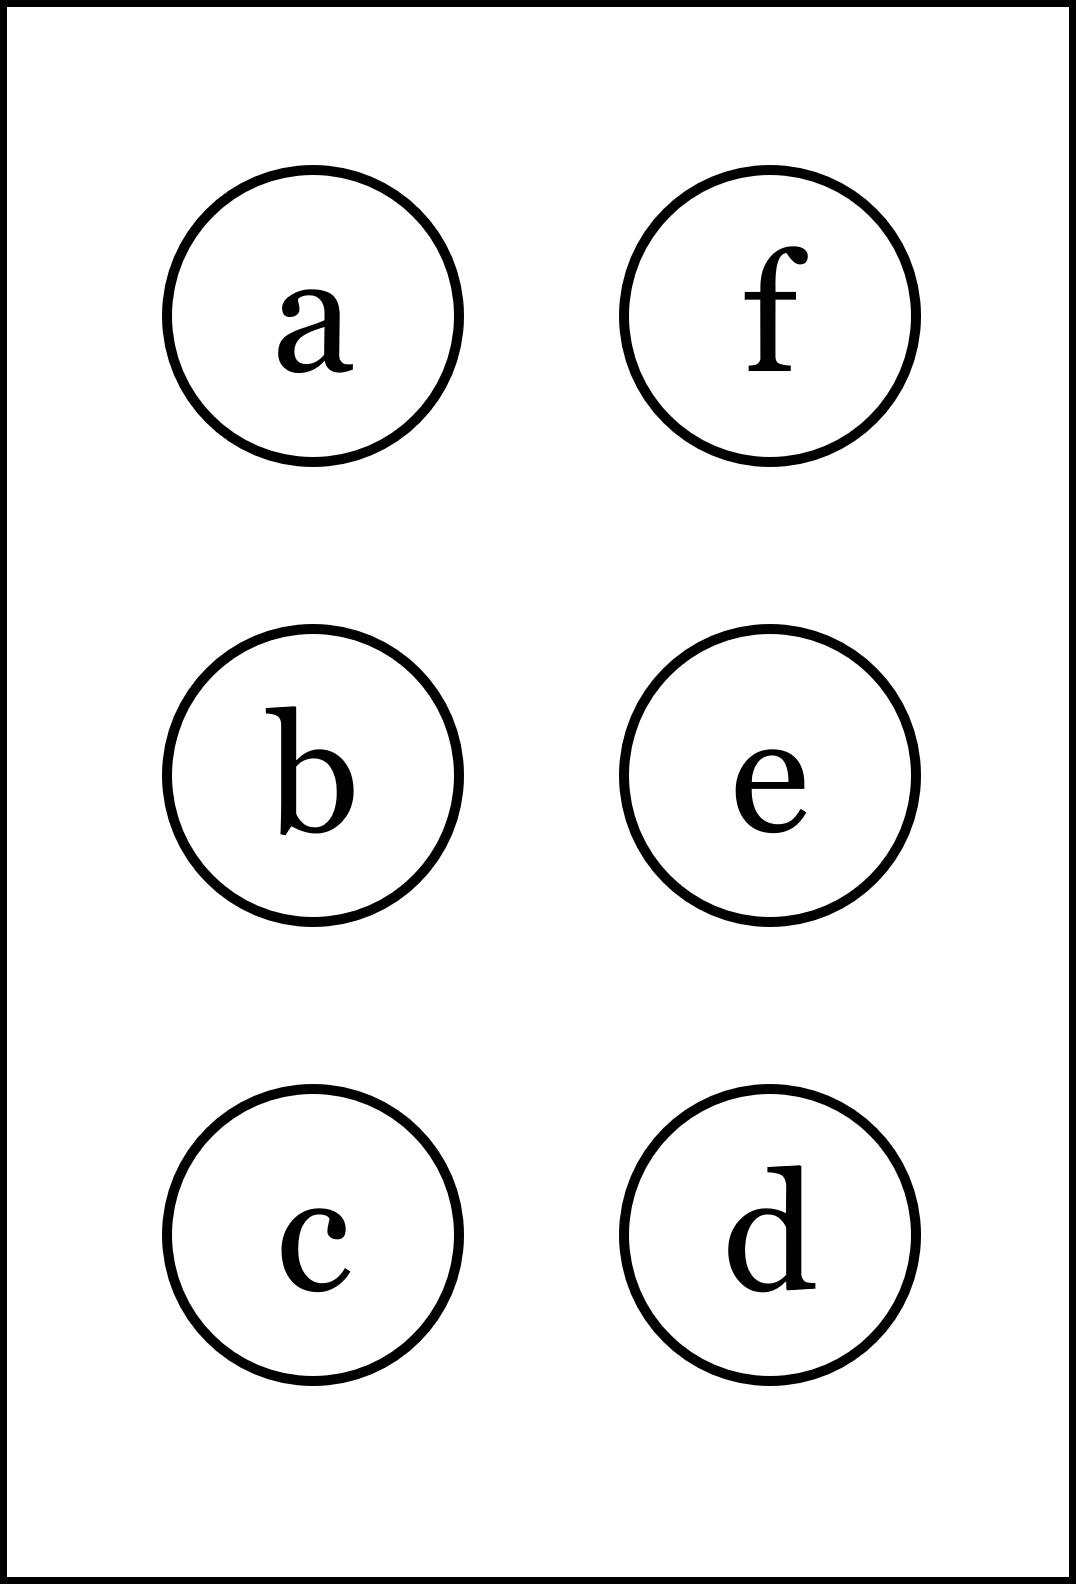
\includegraphics[height=40mm]{../images/braille.png}
{\small Písmeno Braillovej abecedy}
\end{center}
\end{minipage}
\end{center}
\end{minipage}
&
\begin{minipage}[c][104.5mm][t]{0.5\linewidth}
\begin{center}
\vspace{7mm}
{\huge Limity, skupina \textit{Iota $\iota$} -\romannumeral2}\\[5mm]
\textit{Meno:}\phantom{xxxxxxxxxxxxxxxxxxxxxxxxxxxxxxxxxxxxxxxxxxxxxxxxxxxxxxxxxxxxxxxxx}\\[5mm]
\begin{minipage}{0.95\linewidth}
\begin{center}
\textbf{Vypočti limity}. Pokud se výsledky shodujú s tými za otazníky, tak napravo\\obarvi příslušející kroužek načerno. \textbf{Spolu odevzdejte výsledné slovo}.
\end{center}
\end{minipage}
\\[1mm]
\begin{minipage}{0.79\linewidth}
\begin{center}
\begin{varwidth}{\linewidth}
\begin{enumerate}
\normalsize
\item $\lim\limits_{n\to\infty}\cfrac{-4+7n}{-3+6n}$\quad \dotfill\; ???\;\dotfill \quad $\nicefrac{7}{6}$
\item $\lim\limits_{n\to\infty}\cfrac{-7(1+4n)}{(-4n-9)^2}$\quad \dotfill\; ???\;\dotfill \quad $0$
\item $\lim\limits_{n\to\infty}\cfrac{(8-3n)^2}{n^2-6n+5}$\quad \dotfill\; ???\;\dotfill \quad $9$
\item $\lim\limits_{n\to\infty}\cfrac{3^{n+1}}{3^{n-1}}$\quad \dotfill\; ???\;\dotfill \quad $3$
\item $\lim\limits_{n\to\infty}\cfrac{\left(\frac{1}{2}\right)^n -2}{-3n^{6}}$\quad \dotfill\; ???\;\dotfill \quad $\nicefrac{2}{3}$
\item $\lim\limits_{n\to\infty}\cfrac{9\cdot 3^{n+1}-16\cdot 4^{n+1}}{9\cdot 4^{n+2}-4\cdot 3^{n+2}}$\quad \dotfill\; ???\;\dotfill \quad $\nicefrac{-64}{9}$
\end{enumerate}
\end{varwidth}
\end{center}
\end{minipage}
\begin{minipage}{0.20\linewidth}
\begin{center}
{\Huge\bfseries 2.} \\[2mm]
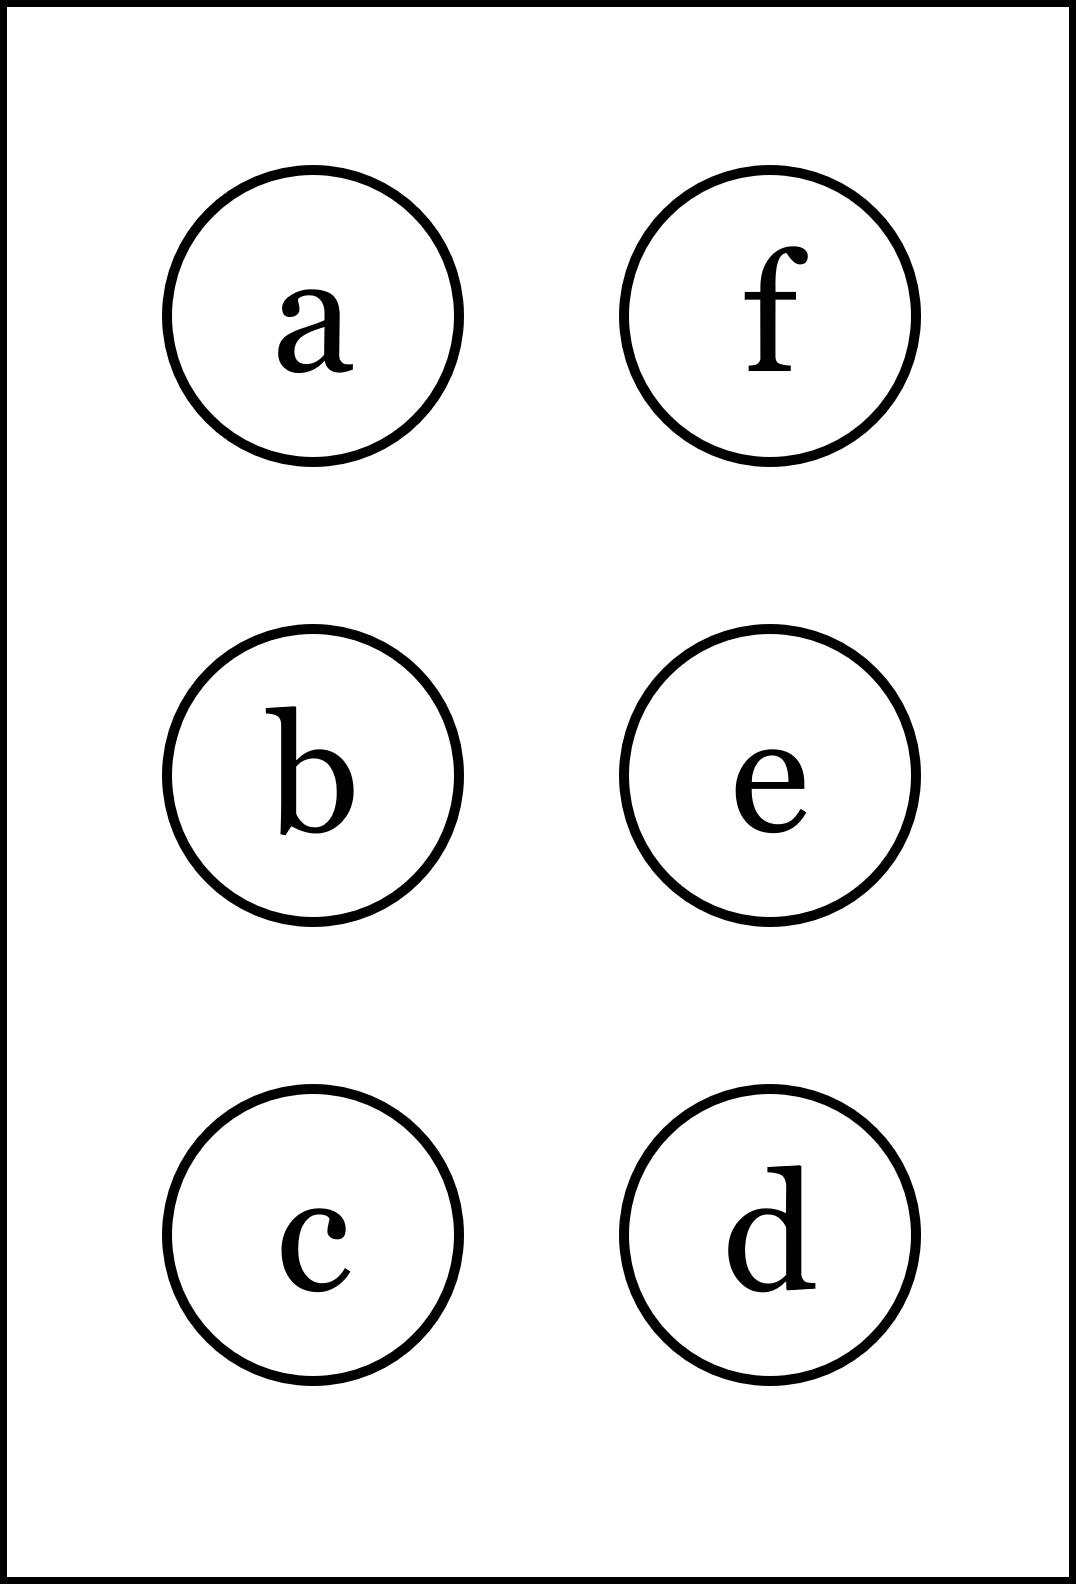
\includegraphics[height=40mm]{../images/braille.png}
{\small Písmeno Braillovej abecedy}
\end{center}
\end{minipage}
\end{center}
\end{minipage}
\\ \hdashline
\begin{minipage}[c][104.5mm][t]{0.5\linewidth}
\begin{center}
\vspace{7mm}
{\huge Limity, skupina \textit{Iota $\iota$} -\romannumeral3}\\[5mm]
\textit{Meno:}\phantom{xxxxxxxxxxxxxxxxxxxxxxxxxxxxxxxxxxxxxxxxxxxxxxxxxxxxxxxxxxxxxxxxx}\\[5mm]
\begin{minipage}{0.95\linewidth}
\begin{center}
\textbf{Vypočti limity}. Pokud se výsledky shodujú s tými za otazníky, tak napravo\\obarvi příslušející kroužek načerno. \textbf{Spolu odevzdejte výsledné slovo}.
\end{center}
\end{minipage}
\\[1mm]
\begin{minipage}{0.79\linewidth}
\begin{center}
\begin{varwidth}{\linewidth}
\begin{enumerate}
\normalsize
\item $\lim\limits_{n\to\infty}\cfrac{-1+5n}{-5+5n}$\quad \dotfill\; ???\;\dotfill \quad $1$
\item $\lim\limits_{n\to\infty}\cfrac{5(-3-n)}{(4n-1)^2}$\quad \dotfill\; ???\;\dotfill \quad $-\infty$
\item $\lim\limits_{n\to\infty}\cfrac{(1-n)^2}{n^2-3n-7}$\quad \dotfill\; ???\;\dotfill \quad $1$
\item $\lim\limits_{n\to\infty}\cfrac{3^{n-2}}{3^{n-1}}$\quad \dotfill\; ???\;\dotfill \quad $0.1111111111111111$
\item $\lim\limits_{n\to\infty}\cfrac{\left(\frac{3}{2}\right)^n -1}{4n^{-4}}$\quad \dotfill\; ???\;\dotfill \quad $\infty$
\item $\lim\limits_{n\to\infty}\cfrac{16\cdot 2^{n+2}-2\cdot 4^{n+1}}{-8\cdot 4^{n-1}-16\cdot 2^{n+2}}$\quad \dotfill\; ???\;\dotfill \quad $\nicefrac{1}{16}$
\end{enumerate}
\end{varwidth}
\end{center}
\end{minipage}
\begin{minipage}{0.20\linewidth}
\begin{center}
{\Huge\bfseries 3.} \\[2mm]
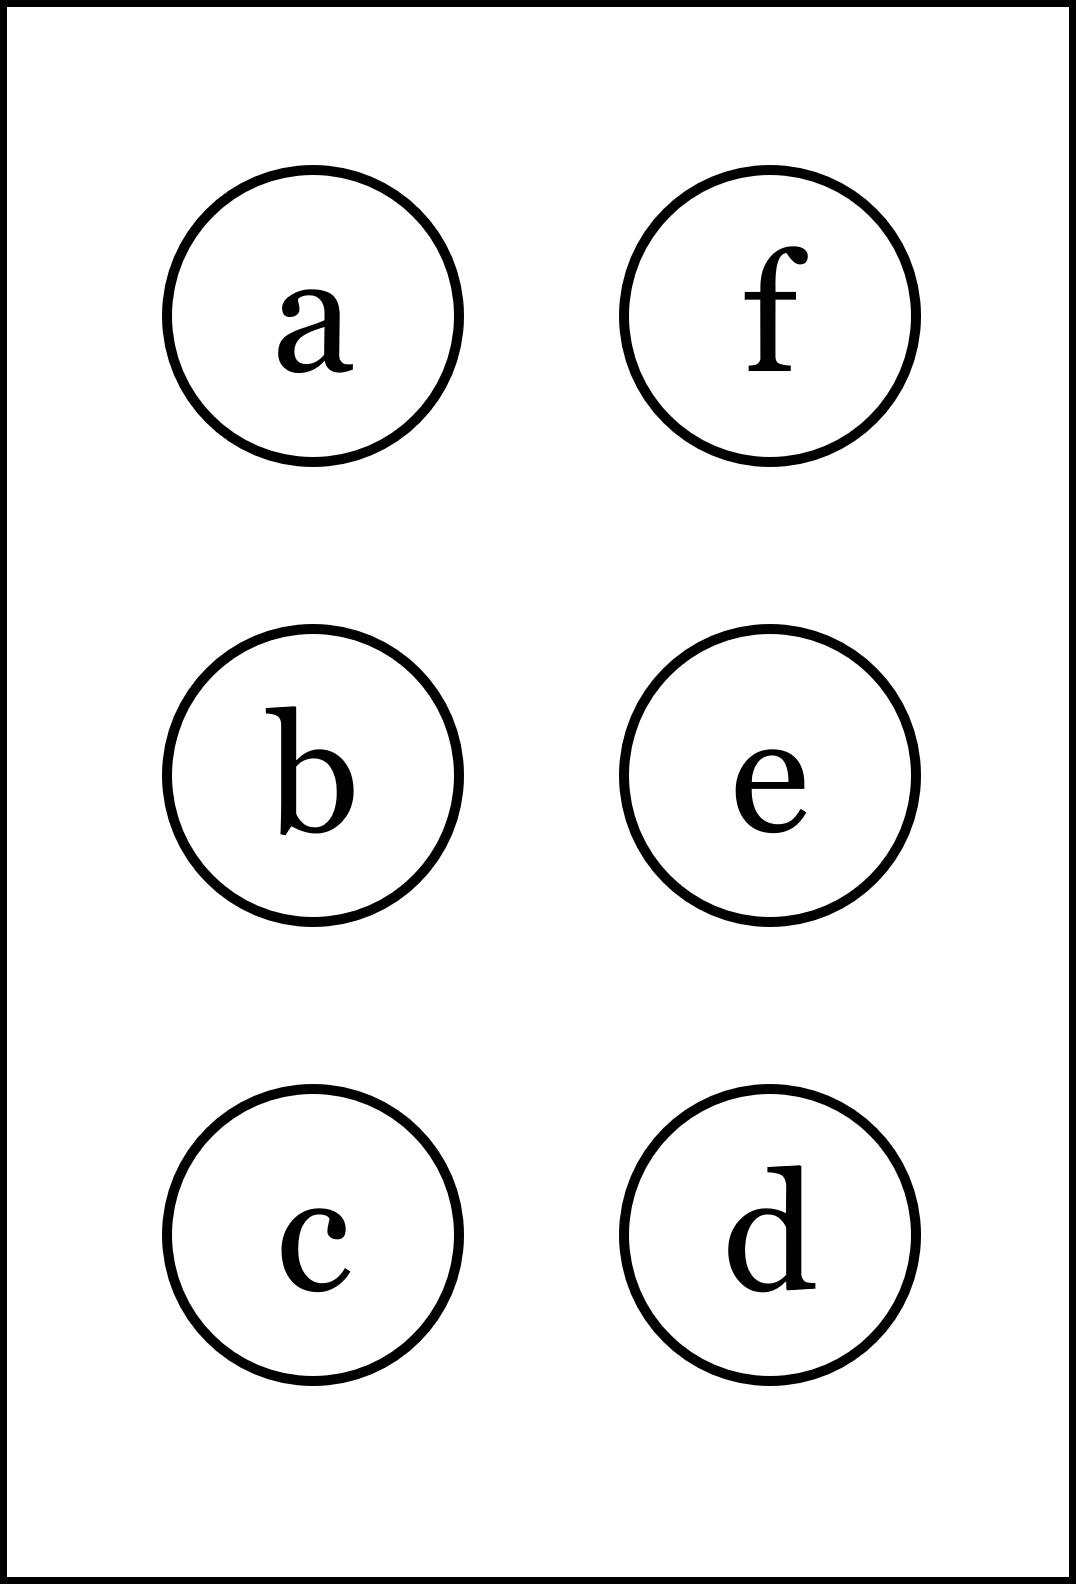
\includegraphics[height=40mm]{../images/braille.png}
{\small Písmeno Braillovej abecedy}
\end{center}
\end{minipage}
\end{center}
\end{minipage}
&
\begin{minipage}[c][104.5mm][t]{0.5\linewidth}
\begin{center}
\vspace{7mm}
{\huge Limity, skupina \textit{Iota $\iota$} -\romannumeral4}\\[5mm]
\textit{Meno:}\phantom{xxxxxxxxxxxxxxxxxxxxxxxxxxxxxxxxxxxxxxxxxxxxxxxxxxxxxxxxxxxxxxxxx}\\[5mm]
\begin{minipage}{0.95\linewidth}
\begin{center}
\textbf{Vypočti limity}. Pokud se výsledky shodujú s tými za otazníky, tak napravo\\obarvi příslušející kroužek načerno. \textbf{Spolu odevzdejte výsledné slovo}.
\end{center}
\end{minipage}
\\[1mm]
\begin{minipage}{0.79\linewidth}
\begin{center}
\begin{varwidth}{\linewidth}
\begin{enumerate}
\normalsize
\item $\lim\limits_{n\to\infty}\cfrac{2-5n}{-6+2n}$\quad \dotfill\; ???\;\dotfill \quad $\nicefrac{-5}{2}$
\item $\lim\limits_{n\to\infty}\cfrac{5(-3-5n)}{(n-1)^2}$\quad \dotfill\; ???\;\dotfill \quad $\infty$
\item $\lim\limits_{n\to\infty}\cfrac{(-8-5n)^2}{n^2+6n-2}$\quad \dotfill\; ???\;\dotfill \quad $25$
\item $\lim\limits_{n\to\infty}\cfrac{3^{n+2}}{3^{n+1}}$\quad \dotfill\; ???\;\dotfill \quad $\infty$
\item $\lim\limits_{n\to\infty}\cfrac{\left(\frac{1}{4}\right)^n +1}{3n^{-8}}$\quad \dotfill\; ???\;\dotfill \quad $\infty$
\item $\lim\limits_{n\to\infty}\cfrac{8\cdot 2^{n+1}+16\cdot 4^{n-2}}{4\cdot 4^{n+1}+4\cdot 2^{n-1}}$\quad \dotfill\; ???\;\dotfill \quad $\nicefrac{1}{16}$
\end{enumerate}
\end{varwidth}
\end{center}
\end{minipage}
\begin{minipage}{0.20\linewidth}
\begin{center}
{\Huge\bfseries 4.} \\[2mm]
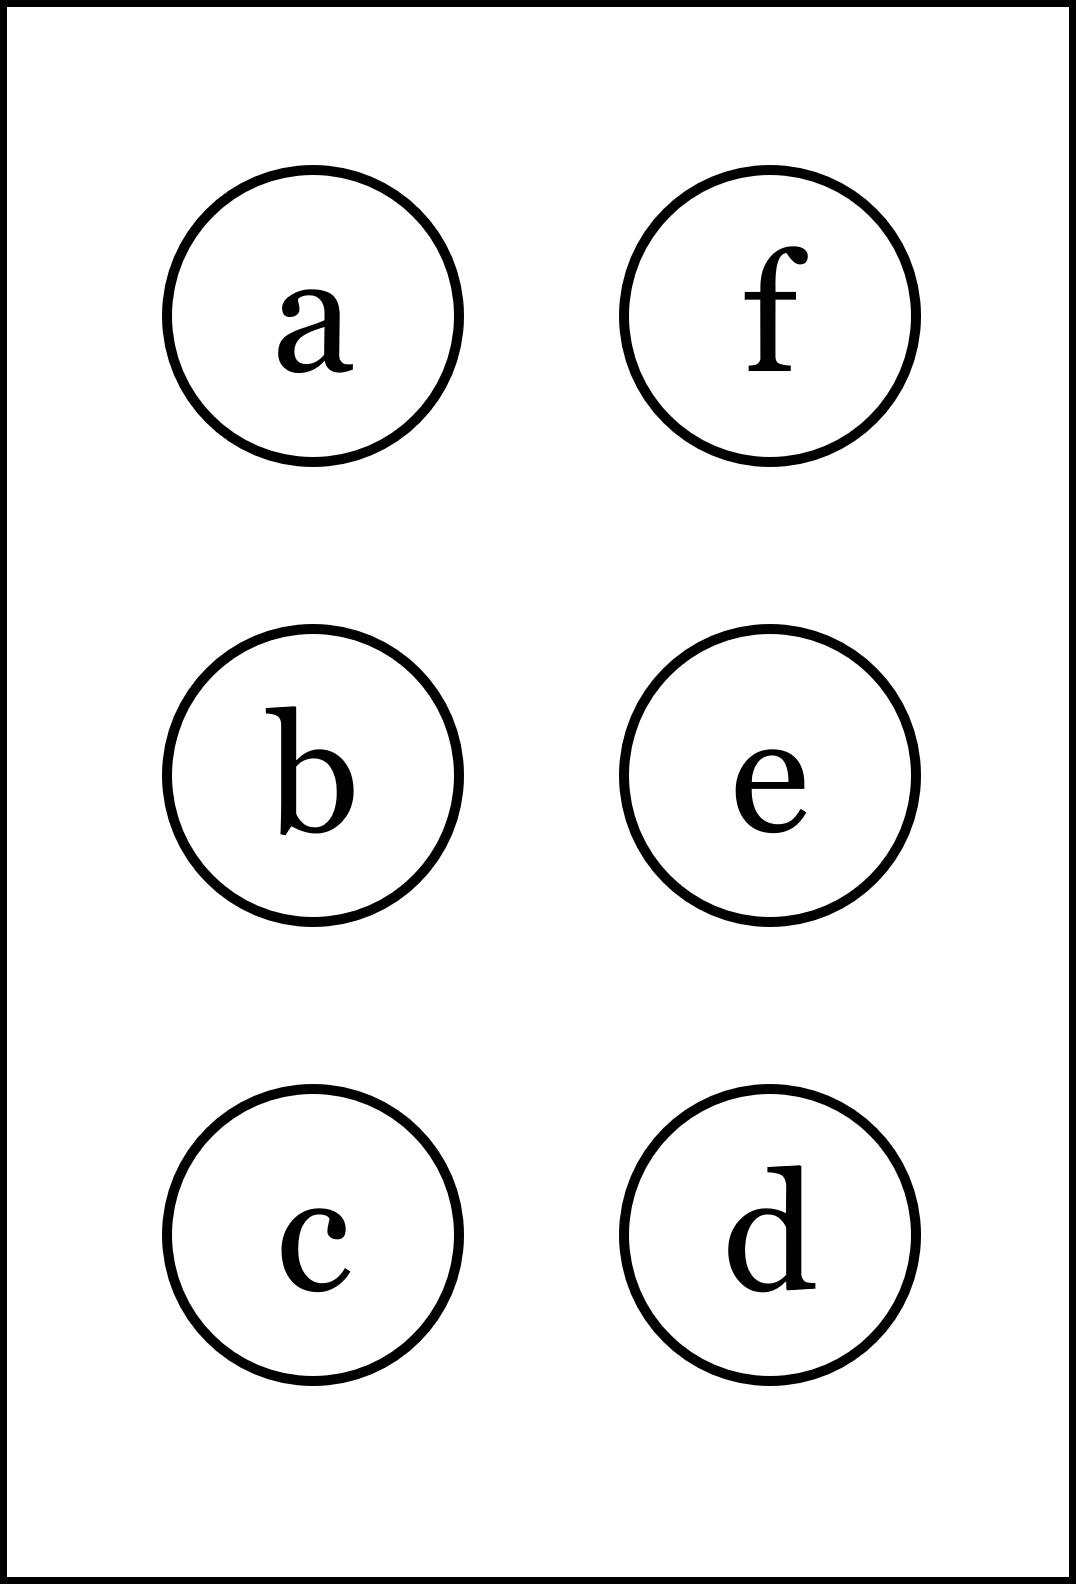
\includegraphics[height=40mm]{../images/braille.png}
{\small Písmeno Braillovej abecedy}
\end{center}
\end{minipage}
\end{center}
\end{minipage}
%
\end{tabular}
\newpage
\thispagestyle{empty}
\begin{tabular}{c:c}
\begin{minipage}[c][104.5mm][t]{0.5\linewidth}
\begin{center}
\vspace{7mm}
{\huge Limity, skupina \textit{Kappa $\kappa$} -\romannumeral1}\\[5mm]
\textit{Meno:}\phantom{xxxxxxxxxxxxxxxxxxxxxxxxxxxxxxxxxxxxxxxxxxxxxxxxxxxxxxxxxxxxxxxxx}\\[5mm]
\begin{minipage}{0.95\linewidth}
\begin{center}
\textbf{Vypočti limity}. Pokud se výsledky shodujú s tými za otazníky, tak napravo\\obarvi příslušející kroužek načerno. \textbf{Spolu odevzdejte výsledné slovo}.
\end{center}
\end{minipage}
\\[1mm]
\begin{minipage}{0.79\linewidth}
\begin{center}
\begin{varwidth}{\linewidth}
\begin{enumerate}
\normalsize
\item $\lim\limits_{n\to\infty}\cfrac{-1-3n}{-1-5n}$\quad \dotfill\; ???\;\dotfill \quad $\nicefrac{3}{5}$
\item $\lim\limits_{n\to\infty}\cfrac{3(-7-5n)}{(-n+2)^2}$\quad \dotfill\; ???\;\dotfill \quad $0$
\item $\lim\limits_{n\to\infty}\cfrac{(-6+7n)^2}{n^2+3n-1}$\quad \dotfill\; ???\;\dotfill \quad $49$
\item $\lim\limits_{n\to\infty}\cfrac{2^{n-3}}{2^{n+1}}$\quad \dotfill\; ???\;\dotfill \quad $16$
\item $\lim\limits_{n\to\infty}\cfrac{\left(\frac{4}{2}\right)^n -2}{-2n^{16}}$\quad \dotfill\; ???\;\dotfill \quad $-\infty$
\item $\lim\limits_{n\to\infty}\cfrac{-3\cdot 2^{n+1}+6\cdot 3^{n-1}}{-4\cdot 3^{n-2}+4\cdot 2^{n+1}}$\quad \dotfill\; ???\;\dotfill \quad $\nicefrac{-1}{2}$
\end{enumerate}
\end{varwidth}
\end{center}
\end{minipage}
\begin{minipage}{0.20\linewidth}
\begin{center}
{\Huge\bfseries 1.} \\[2mm]
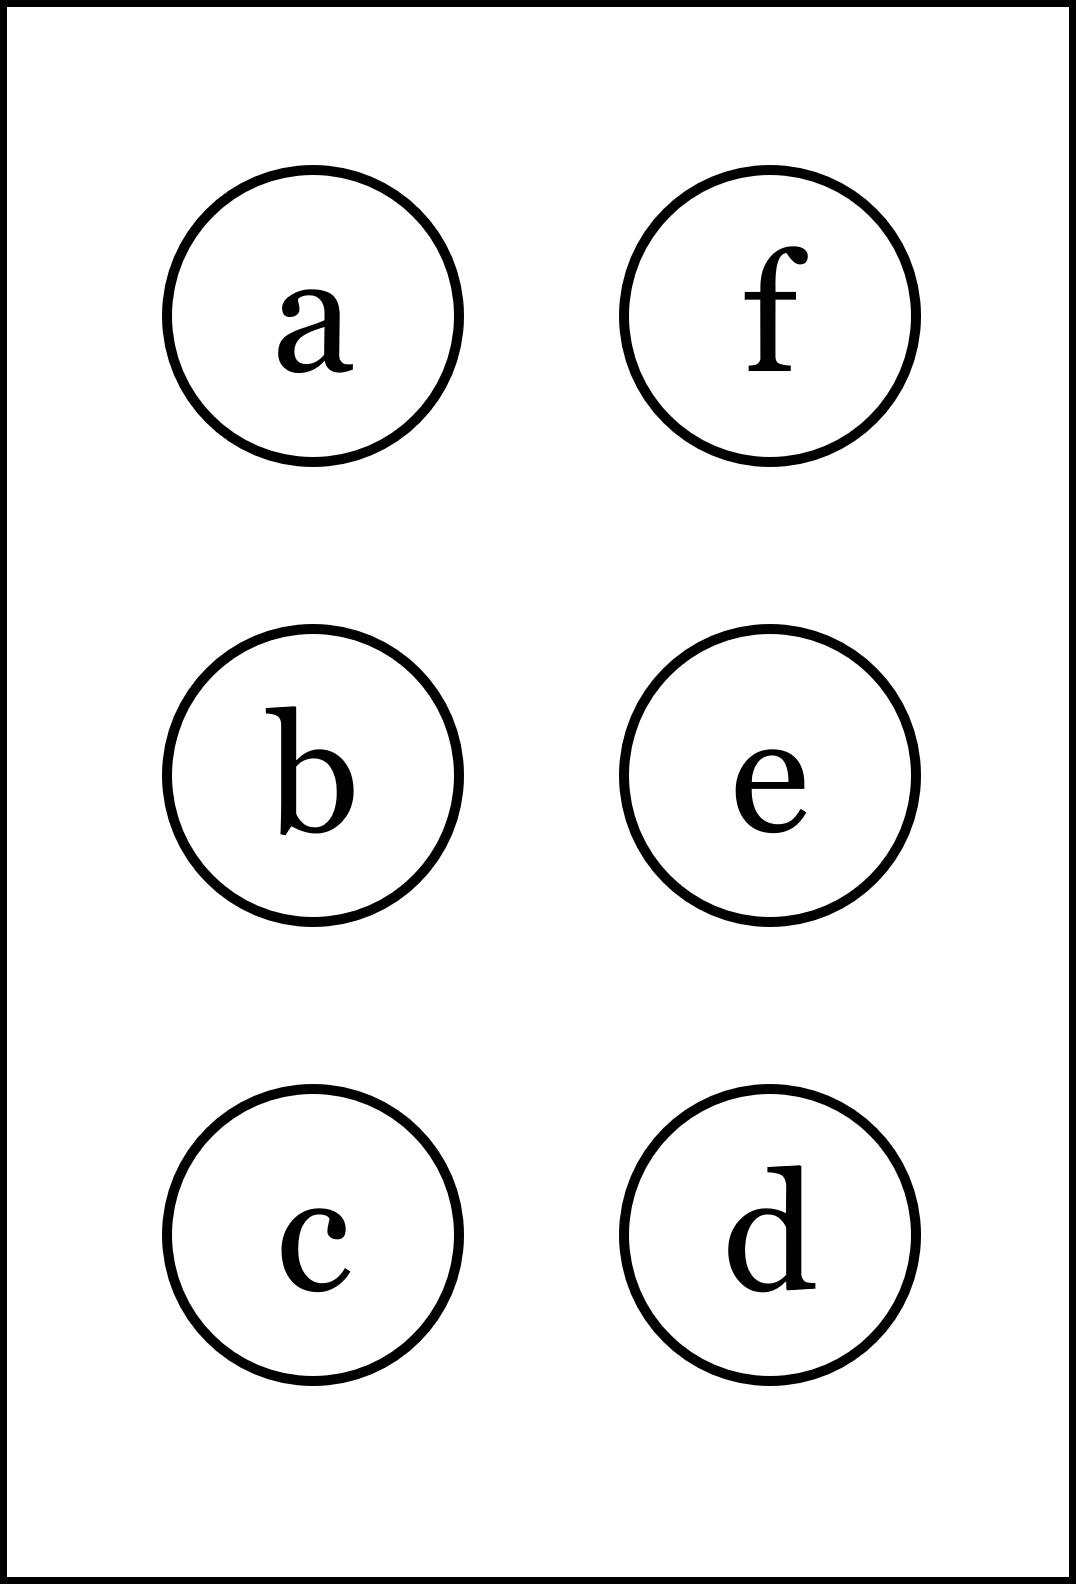
\includegraphics[height=40mm]{../images/braille.png}
{\small Písmeno Braillovej abecedy}
\end{center}
\end{minipage}
\end{center}
\end{minipage}
&
\begin{minipage}[c][104.5mm][t]{0.5\linewidth}
\begin{center}
\vspace{7mm}
{\huge Limity, skupina \textit{Kappa $\kappa$} -\romannumeral2}\\[5mm]
\textit{Meno:}\phantom{xxxxxxxxxxxxxxxxxxxxxxxxxxxxxxxxxxxxxxxxxxxxxxxxxxxxxxxxxxxxxxxxx}\\[5mm]
\begin{minipage}{0.95\linewidth}
\begin{center}
\textbf{Vypočti limity}. Pokud se výsledky shodujú s tými za otazníky, tak napravo\\obarvi příslušející kroužek načerno. \textbf{Spolu odevzdejte výsledné slovo}.
\end{center}
\end{minipage}
\\[1mm]
\begin{minipage}{0.79\linewidth}
\begin{center}
\begin{varwidth}{\linewidth}
\begin{enumerate}
\normalsize
\item $\lim\limits_{n\to\infty}\cfrac{3-3n}{1+7n}$\quad \dotfill\; ???\;\dotfill \quad $\nicefrac{-3}{7}$
\item $\lim\limits_{n\to\infty}\cfrac{-5(-1+2n)}{(3n+2)^2}$\quad \dotfill\; ???\;\dotfill \quad $\nicefrac{1}{6}$
\item $\lim\limits_{n\to\infty}\cfrac{(-4+3n)^2}{n^2+n+7}$\quad \dotfill\; ???\;\dotfill \quad $9$
\item $\lim\limits_{n\to\infty}\cfrac{2^{n+4}}{2^{n+4}}$\quad \dotfill\; ???\;\dotfill \quad $1$
\item $\lim\limits_{n\to\infty}\cfrac{\left(\frac{1}{3}\right)^n -1}{-2n^{-6}}$\quad \dotfill\; ???\;\dotfill \quad $\infty$
\item $\lim\limits_{n\to\infty}\cfrac{6\cdot 2^{n-2}+4\cdot 3^{n+1}}{-3\cdot 3^{n-2}-4\cdot 2^{n-1}}$\quad \dotfill\; ???\;\dotfill \quad $-36$
\end{enumerate}
\end{varwidth}
\end{center}
\end{minipage}
\begin{minipage}{0.20\linewidth}
\begin{center}
{\Huge\bfseries 2.} \\[2mm]
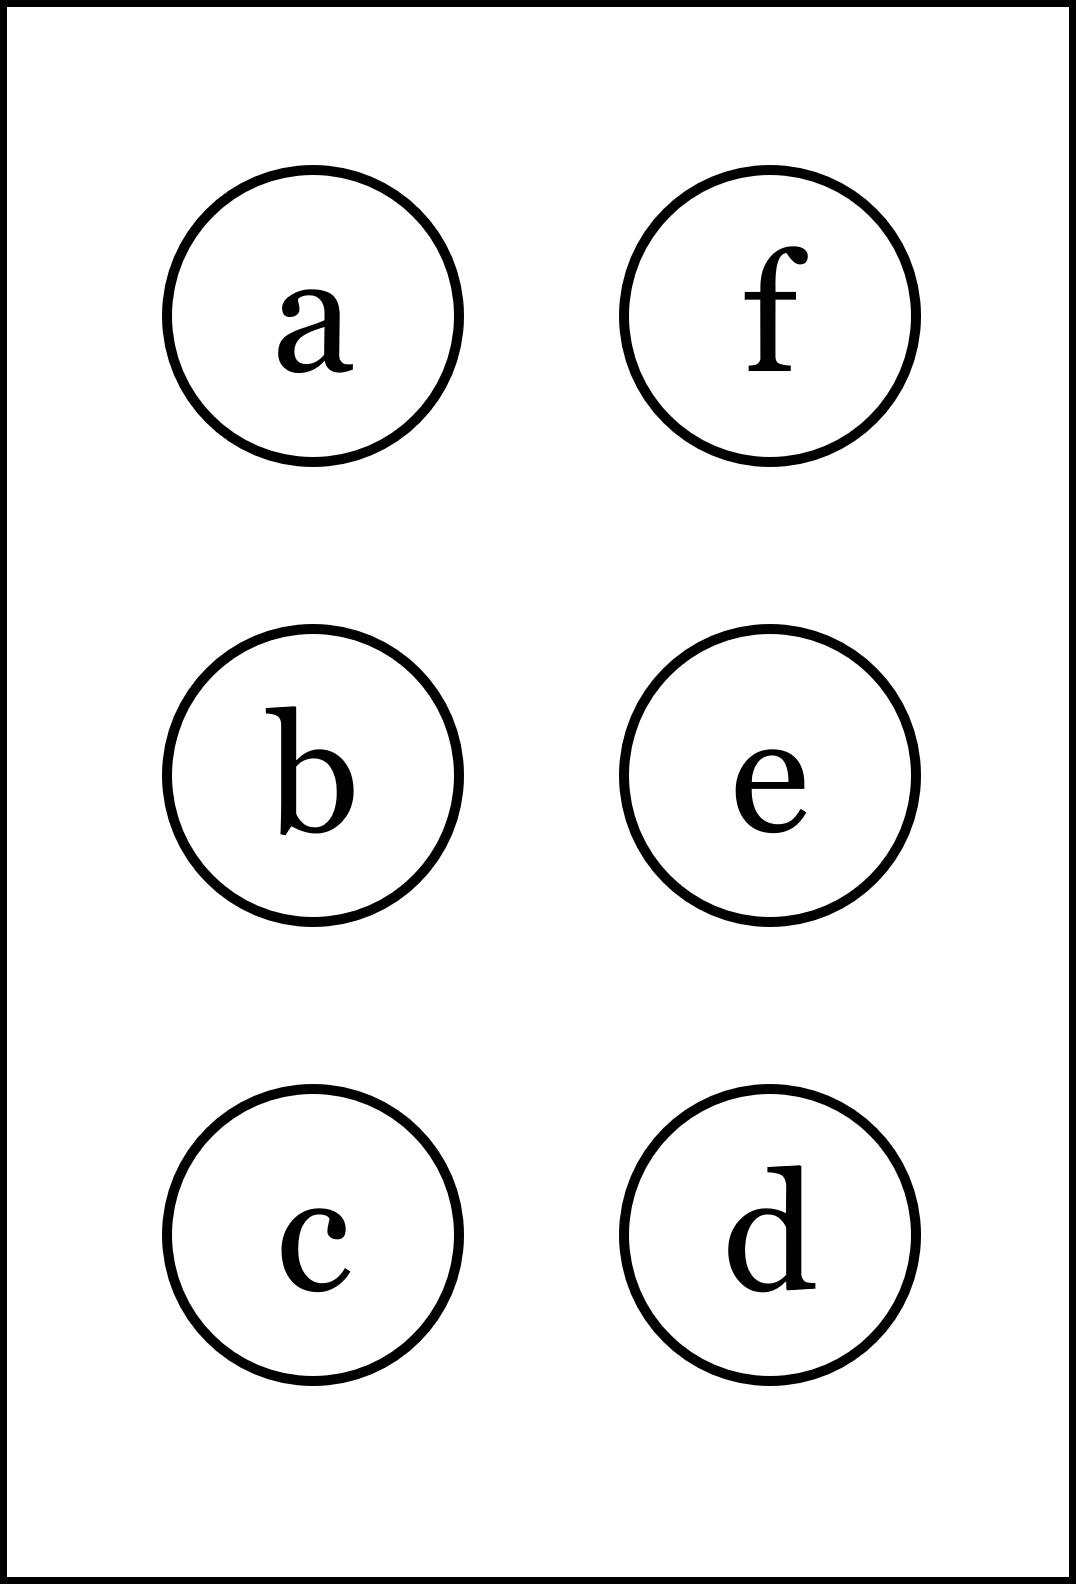
\includegraphics[height=40mm]{../images/braille.png}
{\small Písmeno Braillovej abecedy}
\end{center}
\end{minipage}
\end{center}
\end{minipage}
\\ \hdashline
\begin{minipage}[c][104.5mm][t]{0.5\linewidth}
\begin{center}
\vspace{7mm}
{\huge Limity, skupina \textit{Kappa $\kappa$} -\romannumeral3}\\[5mm]
\textit{Meno:}\phantom{xxxxxxxxxxxxxxxxxxxxxxxxxxxxxxxxxxxxxxxxxxxxxxxxxxxxxxxxxxxxxxxxx}\\[5mm]
\begin{minipage}{0.95\linewidth}
\begin{center}
\textbf{Vypočti limity}. Pokud se výsledky shodujú s tými za otazníky, tak napravo\\obarvi příslušející kroužek načerno. \textbf{Spolu odevzdejte výsledné slovo}.
\end{center}
\end{minipage}
\\[1mm]
\begin{minipage}{0.79\linewidth}
\begin{center}
\begin{varwidth}{\linewidth}
\begin{enumerate}
\normalsize
\item $\lim\limits_{n\to\infty}\cfrac{1+2n}{2-3n}$\quad \dotfill\; ???\;\dotfill \quad $\nicefrac{-2}{3}$
\item $\lim\limits_{n\to\infty}\cfrac{9(-4-n)}{(-3n-1)^2}$\quad \dotfill\; ???\;\dotfill \quad $0$
\item $\lim\limits_{n\to\infty}\cfrac{(-3-2n)^2}{n^2-5n+4}$\quad \dotfill\; ???\;\dotfill \quad $-\infty$
\item $\lim\limits_{n\to\infty}\cfrac{3^{n+1}}{3^{n-2}}$\quad \dotfill\; ???\;\dotfill \quad $-\infty$
\item $\lim\limits_{n\to\infty}\cfrac{\left(\frac{1}{3}\right)^n +2}{2n^{4}}$\quad \dotfill\; ???\;\dotfill \quad $-\infty$
\item $\lim\limits_{n\to\infty}\cfrac{-4\cdot 2^{n+2}-4\cdot 4^{n-1}}{-4\cdot 4^{n+2}+8\cdot 2^{n+1}}$\quad \dotfill\; ???\;\dotfill \quad $4$
\end{enumerate}
\end{varwidth}
\end{center}
\end{minipage}
\begin{minipage}{0.20\linewidth}
\begin{center}
{\Huge\bfseries 3.} \\[2mm]
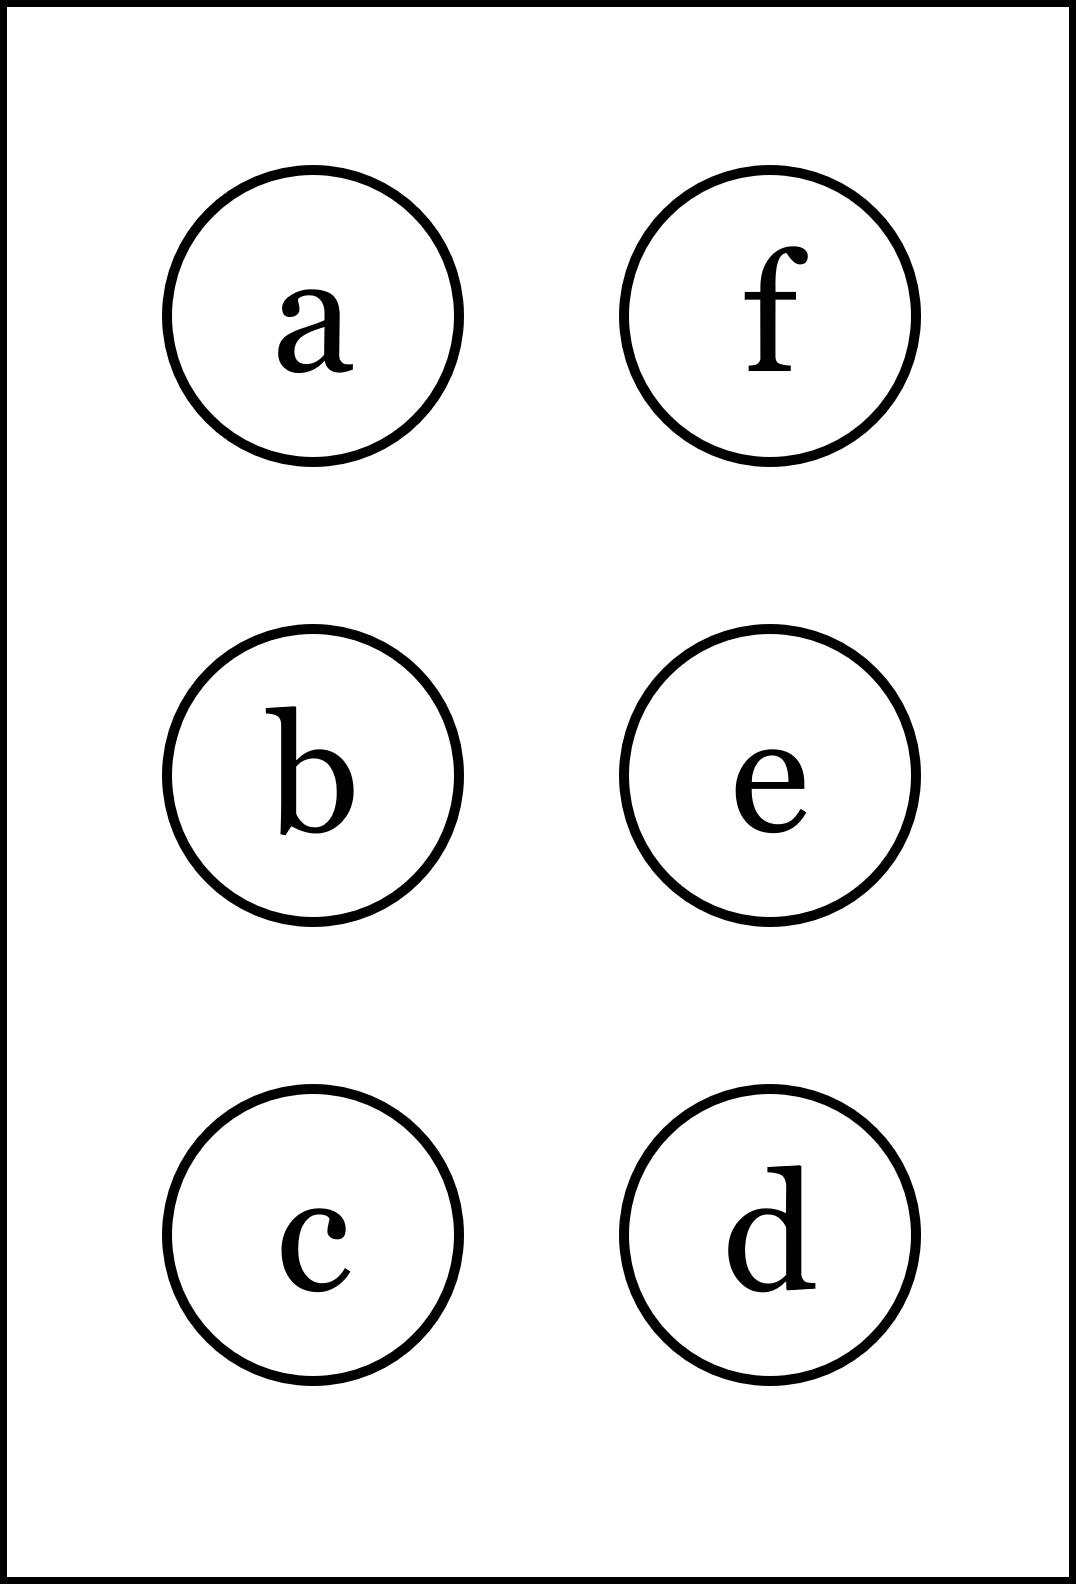
\includegraphics[height=40mm]{../images/braille.png}
{\small Písmeno Braillovej abecedy}
\end{center}
\end{minipage}
\end{center}
\end{minipage}
&
\begin{minipage}[c][104.5mm][t]{0.5\linewidth}
\begin{center}
\vspace{7mm}
{\huge Limity, skupina \textit{Kappa $\kappa$} -\romannumeral4}\\[5mm]
\textit{Meno:}\phantom{xxxxxxxxxxxxxxxxxxxxxxxxxxxxxxxxxxxxxxxxxxxxxxxxxxxxxxxxxxxxxxxxx}\\[5mm]
\begin{minipage}{0.95\linewidth}
\begin{center}
\textbf{Vypočti limity}. Pokud se výsledky shodujú s tými za otazníky, tak napravo\\obarvi příslušející kroužek načerno. \textbf{Spolu odevzdejte výsledné slovo}.
\end{center}
\end{minipage}
\\[1mm]
\begin{minipage}{0.79\linewidth}
\begin{center}
\begin{varwidth}{\linewidth}
\begin{enumerate}
\normalsize
\item $\lim\limits_{n\to\infty}\cfrac{4+2n}{8-9n}$\quad \dotfill\; ???\;\dotfill \quad $\nicefrac{-2}{9}$
\item $\lim\limits_{n\to\infty}\cfrac{1(-6+2n)}{(-9n+1)^2}$\quad \dotfill\; ???\;\dotfill \quad $\nicefrac{-2}{9}$
\item $\lim\limits_{n\to\infty}\cfrac{(2-4n)^2}{n^2-2n-3}$\quad \dotfill\; ???\;\dotfill \quad $\infty$
\item $\lim\limits_{n\to\infty}\cfrac{3^{n+3}}{3^{n-1}}$\quad \dotfill\; ???\;\dotfill \quad $\nicefrac{1}{81}$
\item $\lim\limits_{n\to\infty}\cfrac{\left(\frac{1}{2}\right)^n -1}{-n^{-6}}$\quad \dotfill\; ???\;\dotfill \quad $-6$
\item $\lim\limits_{n\to\infty}\cfrac{4\cdot 2^{n-1}-4\cdot 4^{n-1}}{-8\cdot 4^{n-2}-8\cdot 2^{n+1}}$\quad \dotfill\; ???\;\dotfill \quad $\nicefrac{1}{8}$
\end{enumerate}
\end{varwidth}
\end{center}
\end{minipage}
\begin{minipage}{0.20\linewidth}
\begin{center}
{\Huge\bfseries 4.} \\[2mm]
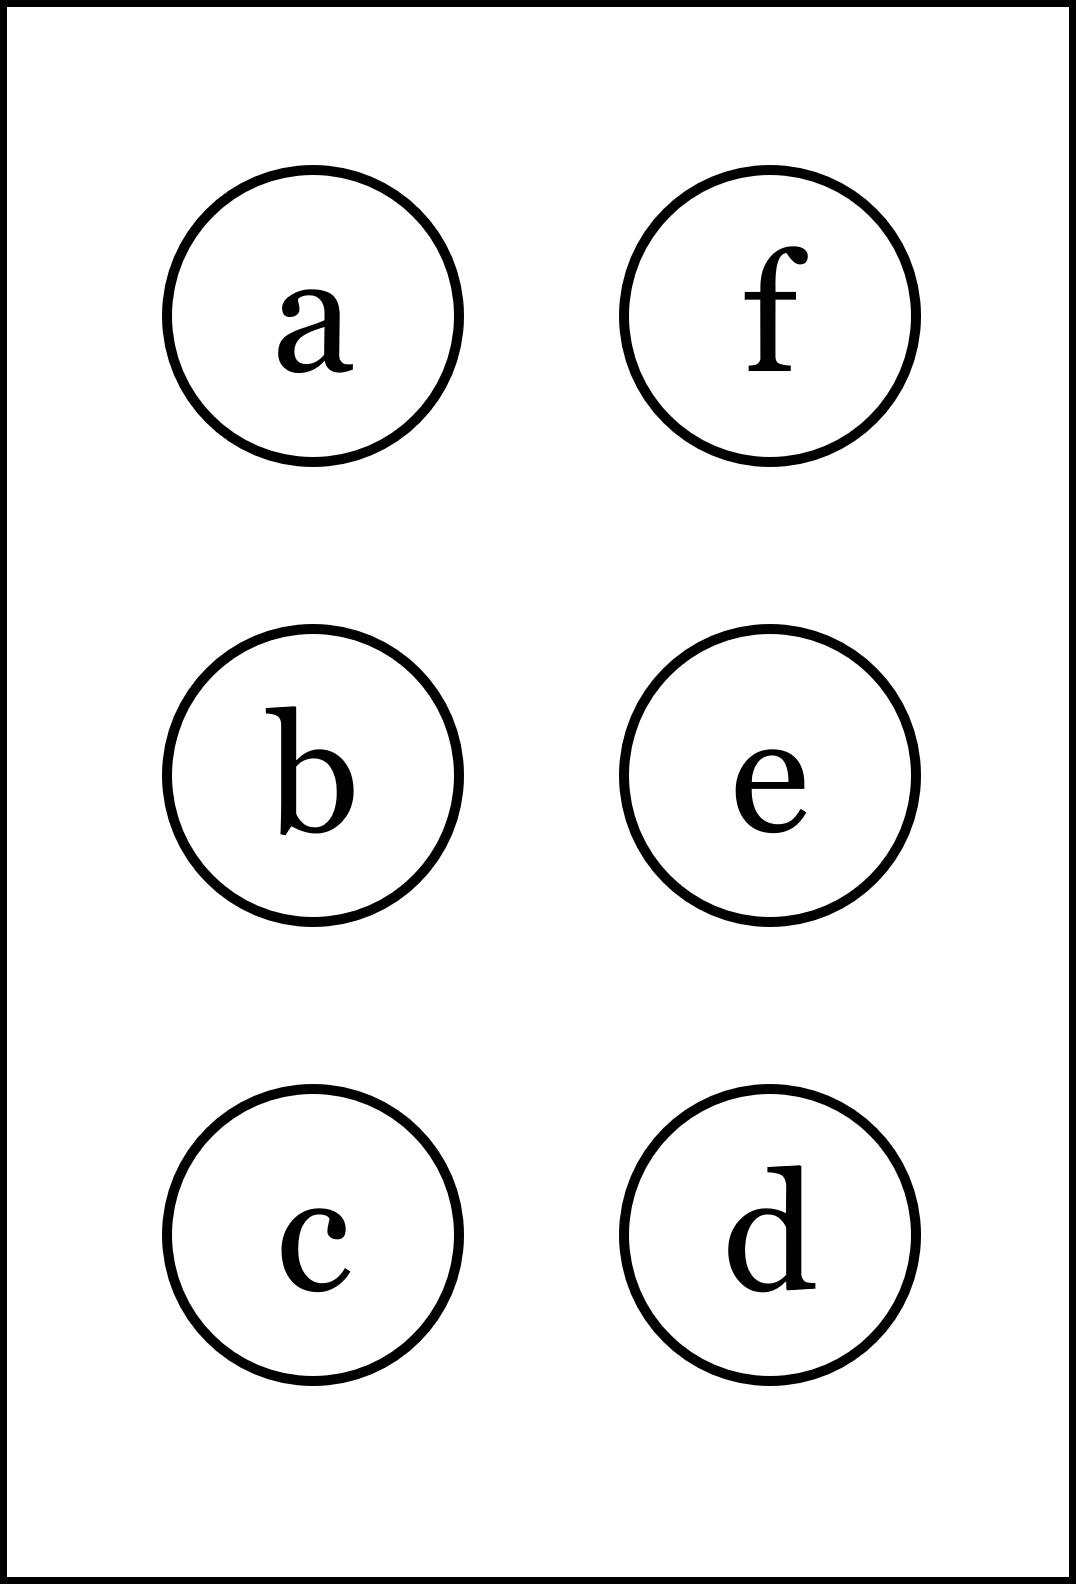
\includegraphics[height=40mm]{../images/braille.png}
{\small Písmeno Braillovej abecedy}
\end{center}
\end{minipage}
\end{center}
\end{minipage}
%
\end{tabular}
\newpage
\thispagestyle{empty}
\begin{tabular}{c:c}
\begin{minipage}[c][104.5mm][t]{0.5\linewidth}
\begin{center}
\vspace{7mm}
{\huge Limity, skupina \textit{Lambda $\lambda$} -\romannumeral1}\\[5mm]
\textit{Meno:}\phantom{xxxxxxxxxxxxxxxxxxxxxxxxxxxxxxxxxxxxxxxxxxxxxxxxxxxxxxxxxxxxxxxxx}\\[5mm]
\begin{minipage}{0.95\linewidth}
\begin{center}
\textbf{Vypočti limity}. Pokud se výsledky shodujú s tými za otazníky, tak napravo\\obarvi příslušející kroužek načerno. \textbf{Spolu odevzdejte výsledné slovo}.
\end{center}
\end{minipage}
\\[1mm]
\begin{minipage}{0.79\linewidth}
\begin{center}
\begin{varwidth}{\linewidth}
\begin{enumerate}
\normalsize
\item $\lim\limits_{n\to\infty}\cfrac{-1-3n}{1+4n}$\quad \dotfill\; ???\;\dotfill \quad $\nicefrac{-3}{4}$
\item $\lim\limits_{n\to\infty}\cfrac{3(5+5n)}{(-3n-3)^2}$\quad \dotfill\; ???\;\dotfill \quad $0$
\item $\lim\limits_{n\to\infty}\cfrac{(-1+4n)^2}{n^2-2n+3}$\quad \dotfill\; ???\;\dotfill \quad $16$
\item $\lim\limits_{n\to\infty}\cfrac{2^{n-1}}{2^{n+1}}$\quad \dotfill\; ???\;\dotfill \quad $\nicefrac{1}{4}$
\item $\lim\limits_{n\to\infty}\cfrac{\left(\frac{3}{4}\right)^n +1}{3n^{-4}}$\quad \dotfill\; ???\;\dotfill \quad $\nicefrac{1}{3}$
\item $\lim\limits_{n\to\infty}\cfrac{-3\cdot 2^{n+2}-9\cdot 3^{n-2}}{2\cdot 3^{n-1}+2\cdot 2^{n-2}}$\quad \dotfill\; ???\;\dotfill \quad $\nicefrac{-27}{2}$
\end{enumerate}
\end{varwidth}
\end{center}
\end{minipage}
\begin{minipage}{0.20\linewidth}
\begin{center}
{\Huge\bfseries 1.} \\[2mm]
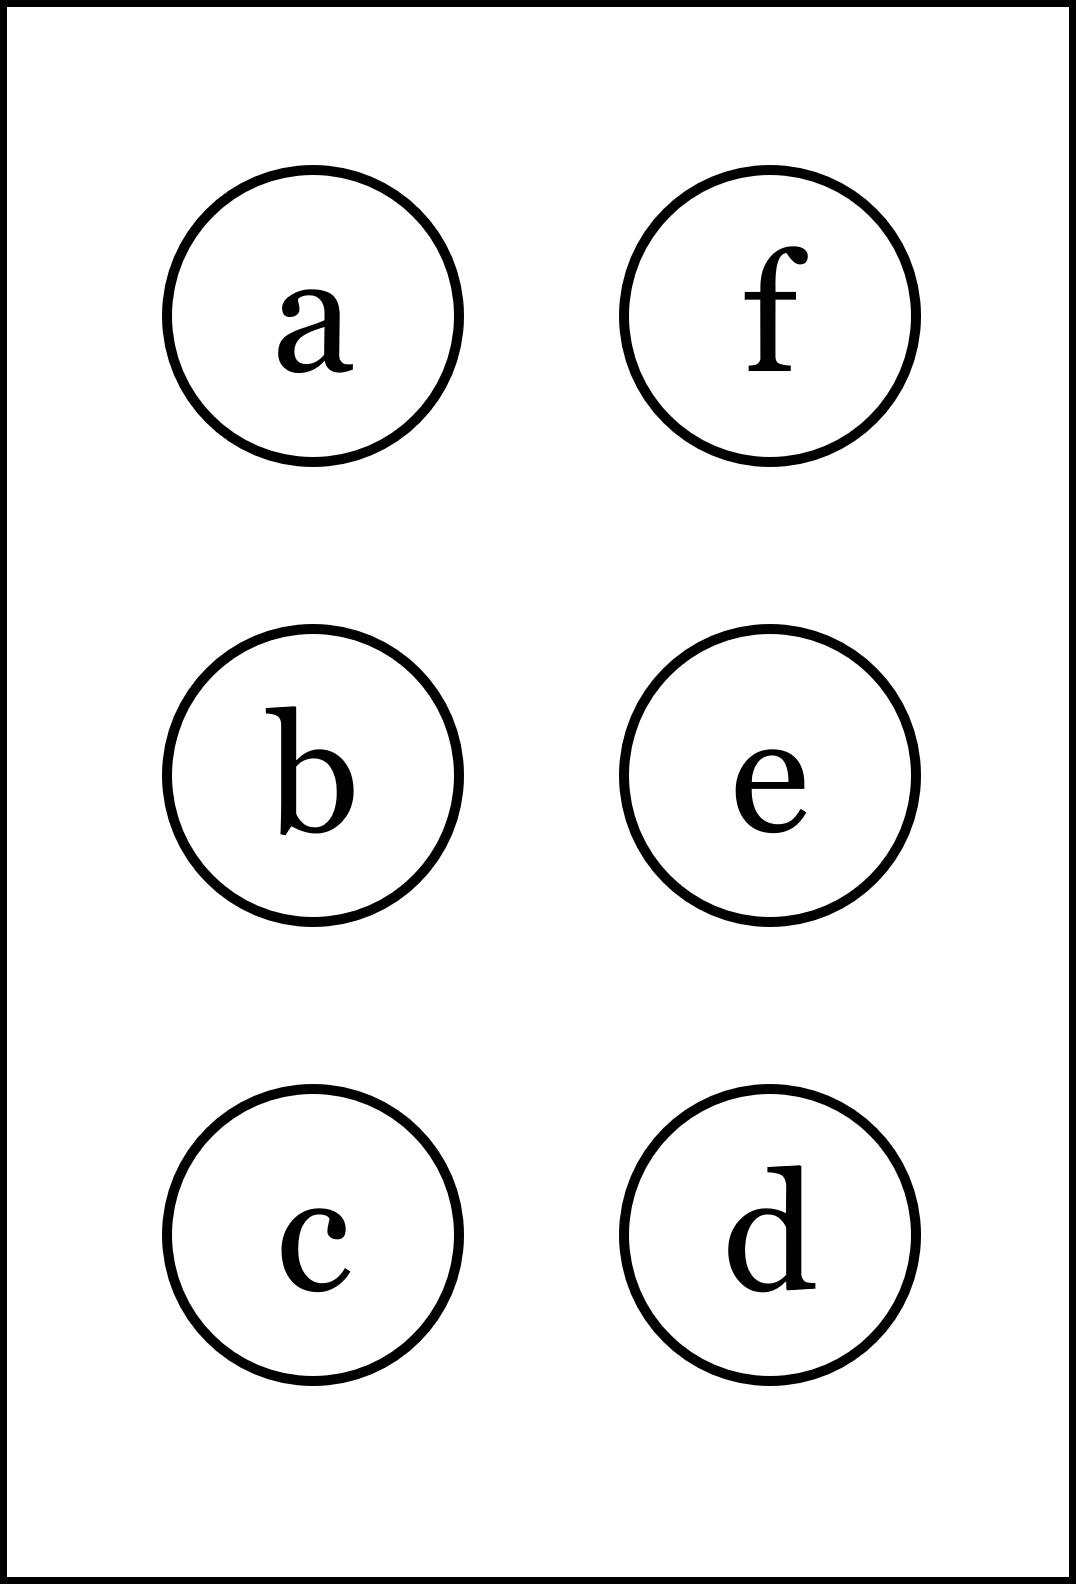
\includegraphics[height=40mm]{../images/braille.png}
{\small Písmeno Braillovej abecedy}
\end{center}
\end{minipage}
\end{center}
\end{minipage}
&
\begin{minipage}[c][104.5mm][t]{0.5\linewidth}
\begin{center}
\vspace{7mm}
{\huge Limity, skupina \textit{Lambda $\lambda$} -\romannumeral2}\\[5mm]
\textit{Meno:}\phantom{xxxxxxxxxxxxxxxxxxxxxxxxxxxxxxxxxxxxxxxxxxxxxxxxxxxxxxxxxxxxxxxxx}\\[5mm]
\begin{minipage}{0.95\linewidth}
\begin{center}
\textbf{Vypočti limity}. Pokud se výsledky shodujú s tými za otazníky, tak napravo\\obarvi příslušející kroužek načerno. \textbf{Spolu odevzdejte výsledné slovo}.
\end{center}
\end{minipage}
\\[1mm]
\begin{minipage}{0.79\linewidth}
\begin{center}
\begin{varwidth}{\linewidth}
\begin{enumerate}
\normalsize
\item $\lim\limits_{n\to\infty}\cfrac{-7+4n}{1+6n}$\quad \dotfill\; ???\;\dotfill \quad $\nicefrac{2}{3}$
\item $\lim\limits_{n\to\infty}\cfrac{7(7+2n)}{(3n+3)^2}$\quad \dotfill\; ???\;\dotfill \quad $0$
\item $\lim\limits_{n\to\infty}\cfrac{(5+5n)^2}{n^2-5n-6}$\quad \dotfill\; ???\;\dotfill \quad $25$
\item $\lim\limits_{n\to\infty}\cfrac{2^{n-2}}{2^{n-1}}$\quad \dotfill\; ???\;\dotfill \quad $0.25$
\item $\lim\limits_{n\to\infty}\cfrac{\left(\frac{4}{3}\right)^n -4}{n^{-8}}$\quad \dotfill\; ???\;\dotfill \quad $-4$
\item $\lim\limits_{n\to\infty}\cfrac{-4\cdot 2^{n-2}-4\cdot 4^{n+2}}{4\cdot 4^{n+2}-8\cdot 2^{n+2}}$\quad \dotfill\; ???\;\dotfill \quad $\nicefrac{-1}{2}$
\end{enumerate}
\end{varwidth}
\end{center}
\end{minipage}
\begin{minipage}{0.20\linewidth}
\begin{center}
{\Huge\bfseries 2.} \\[2mm]
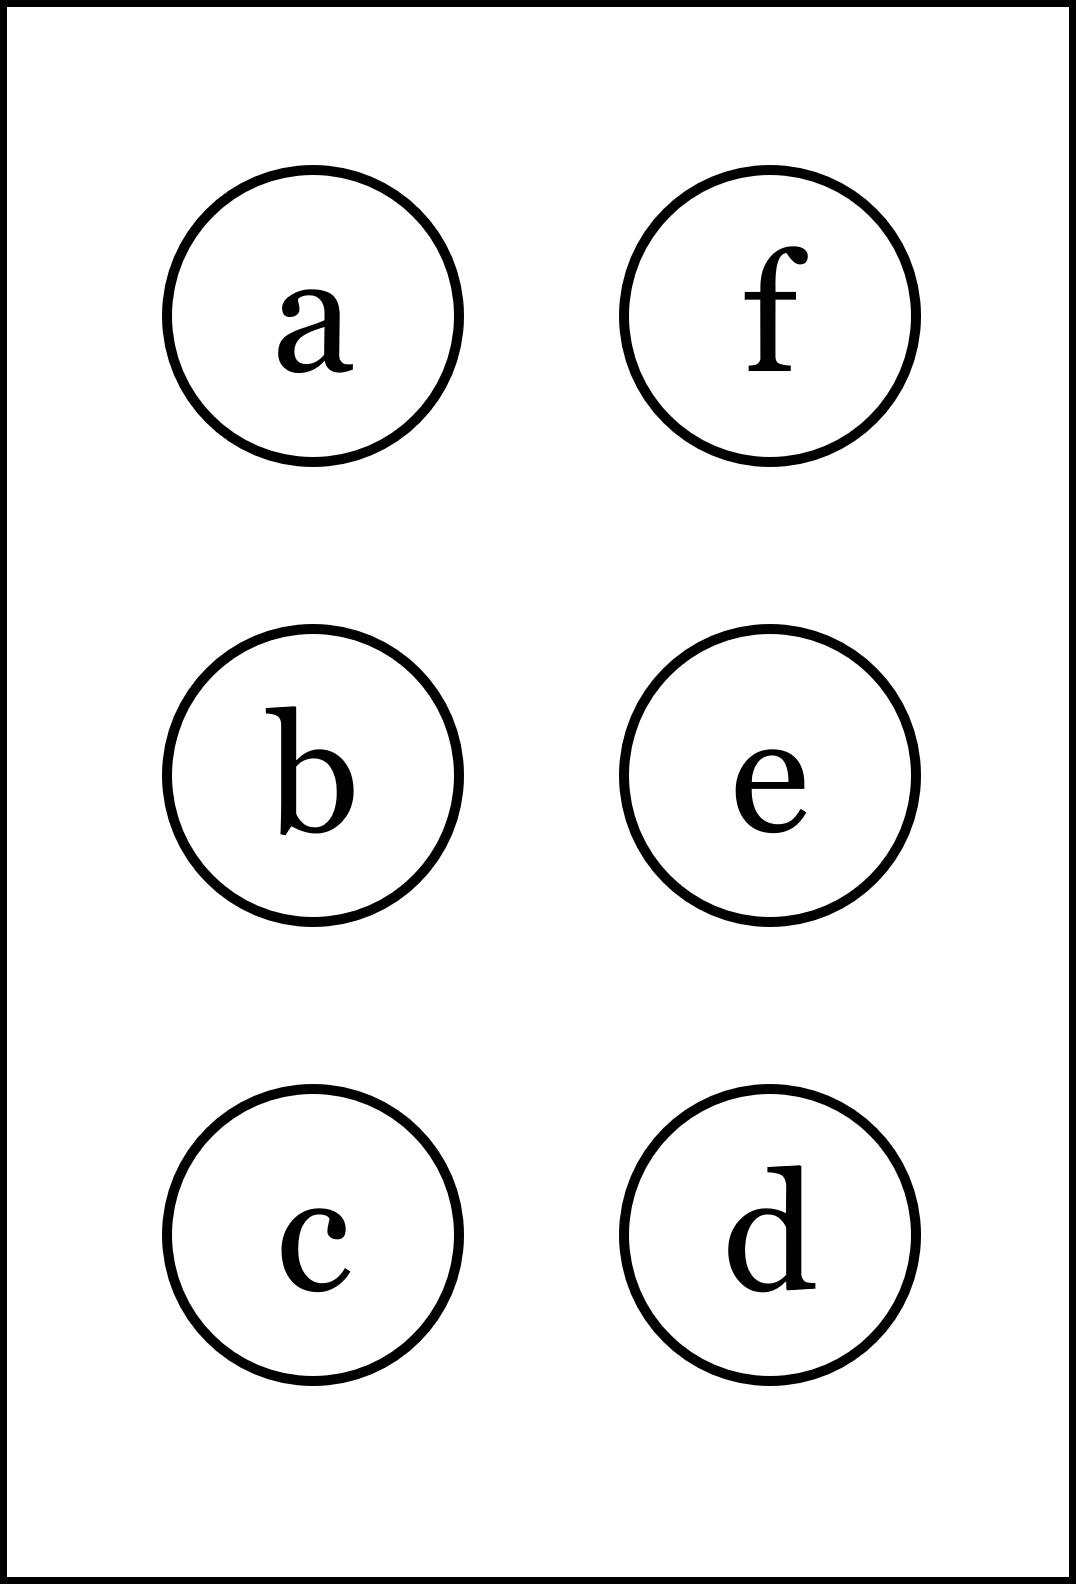
\includegraphics[height=40mm]{../images/braille.png}
{\small Písmeno Braillovej abecedy}
\end{center}
\end{minipage}
\end{center}
\end{minipage}
\\ \hdashline
\begin{minipage}[c][104.5mm][t]{0.5\linewidth}
\begin{center}
\vspace{7mm}
{\huge Limity, skupina \textit{Lambda $\lambda$} -\romannumeral3}\\[5mm]
\textit{Meno:}\phantom{xxxxxxxxxxxxxxxxxxxxxxxxxxxxxxxxxxxxxxxxxxxxxxxxxxxxxxxxxxxxxxxxx}\\[5mm]
\begin{minipage}{0.95\linewidth}
\begin{center}
\textbf{Vypočti limity}. Pokud se výsledky shodujú s tými za otazníky, tak napravo\\obarvi příslušející kroužek načerno. \textbf{Spolu odevzdejte výsledné slovo}.
\end{center}
\end{minipage}
\\[1mm]
\begin{minipage}{0.79\linewidth}
\begin{center}
\begin{varwidth}{\linewidth}
\begin{enumerate}
\normalsize
\item $\lim\limits_{n\to\infty}\cfrac{-9-4n}{-2+6n}$\quad \dotfill\; ???\;\dotfill \quad $\nicefrac{-2}{3}$
\item $\lim\limits_{n\to\infty}\cfrac{3(5-3n)}{(n-5)^2}$\quad \dotfill\; ???\;\dotfill \quad $\infty$
\item $\lim\limits_{n\to\infty}\cfrac{(1+2n)^2}{n^2+2n-3}$\quad \dotfill\; ???\;\dotfill \quad $\nicefrac{-1}{3}$
\item $\lim\limits_{n\to\infty}\cfrac{3^{n+2}}{3^{n+1}}$\quad \dotfill\; ???\;\dotfill \quad $-\infty$
\item $\lim\limits_{n\to\infty}\cfrac{\left(\frac{1}{2}\right)^n -1}{-2n^{6}}$\quad \dotfill\; ???\;\dotfill \quad $\nicefrac{1}{2}$
\item $\lim\limits_{n\to\infty}\cfrac{4\cdot 2^{n-1}+4\cdot 4^{n+1}}{8\cdot 4^{n-1}+16\cdot 2^{n-2}}$\quad \dotfill\; ???\;\dotfill \quad $\nicefrac{1}{8}$
\end{enumerate}
\end{varwidth}
\end{center}
\end{minipage}
\begin{minipage}{0.20\linewidth}
\begin{center}
{\Huge\bfseries 3.} \\[2mm]
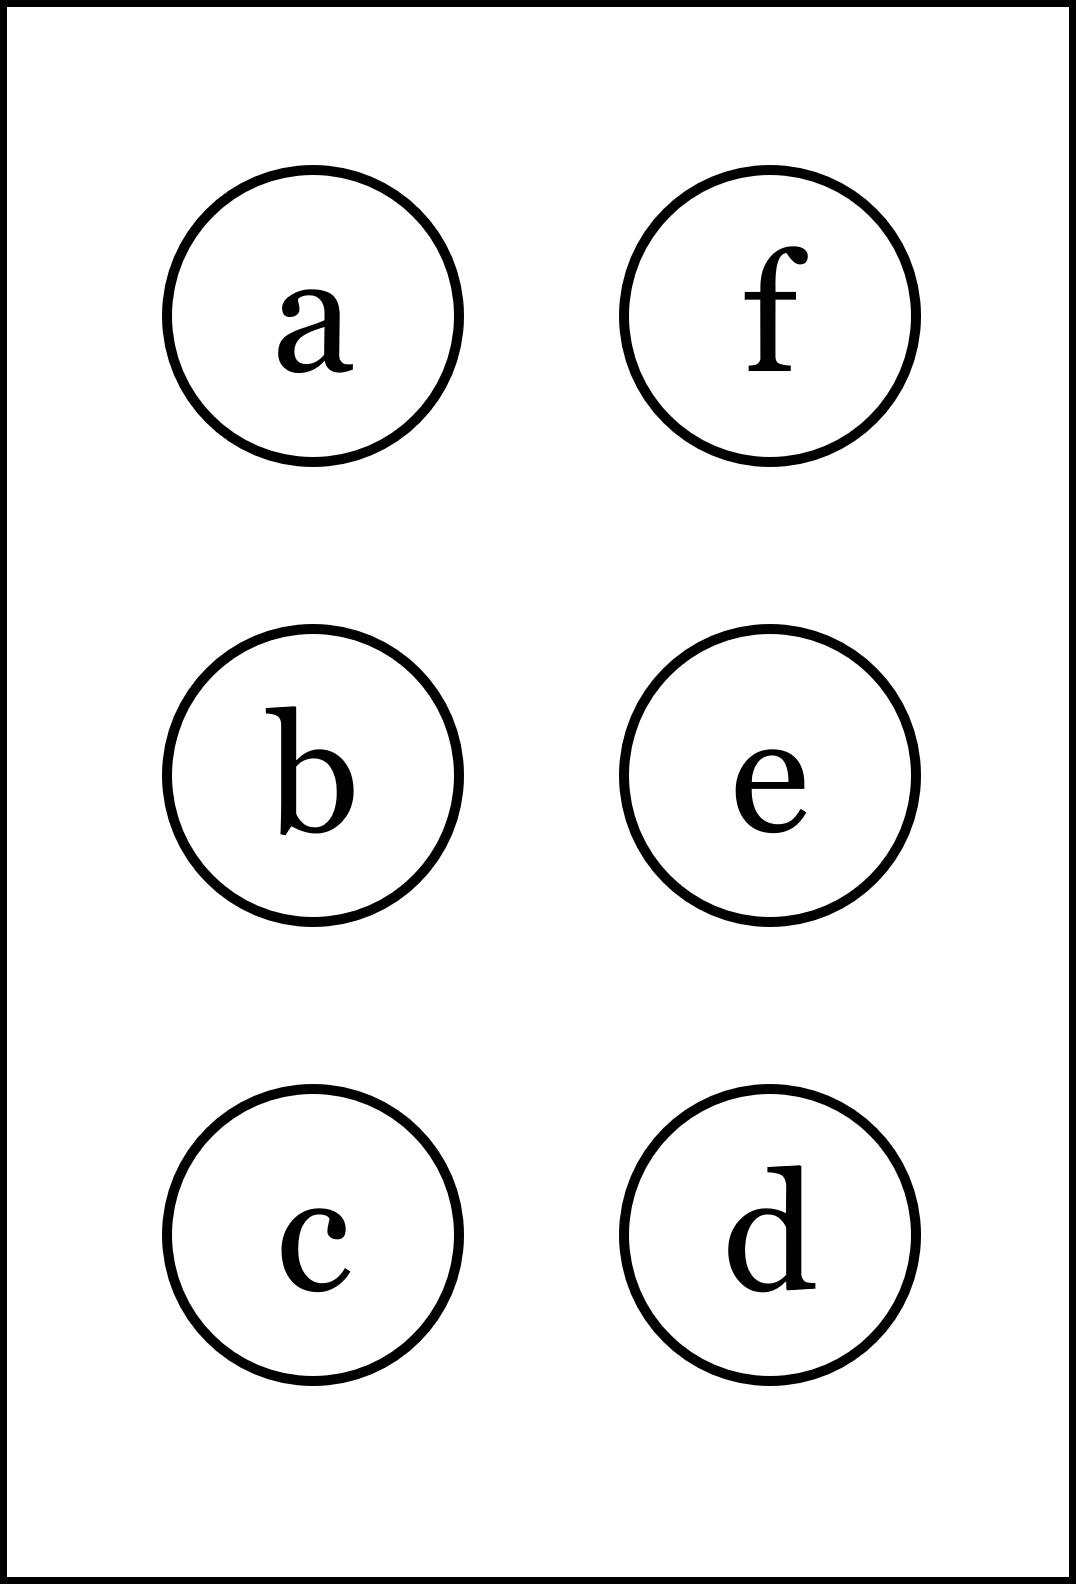
\includegraphics[height=40mm]{../images/braille.png}
{\small Písmeno Braillovej abecedy}
\end{center}
\end{minipage}
\end{center}
\end{minipage}
&
\begin{minipage}[c][104.5mm][t]{0.5\linewidth}
\begin{center}
\vspace{7mm}
{\huge Limity, skupina \textit{Lambda $\lambda$} -\romannumeral4}\\[5mm]
\textit{Meno:}\phantom{xxxxxxxxxxxxxxxxxxxxxxxxxxxxxxxxxxxxxxxxxxxxxxxxxxxxxxxxxxxxxxxxx}\\[5mm]
\begin{minipage}{0.95\linewidth}
\begin{center}
\textbf{Vypočti limity}. Pokud se výsledky shodujú s tými za otazníky, tak napravo\\obarvi příslušející kroužek načerno. \textbf{Spolu odevzdejte výsledné slovo}.
\end{center}
\end{minipage}
\\[1mm]
\begin{minipage}{0.79\linewidth}
\begin{center}
\begin{varwidth}{\linewidth}
\begin{enumerate}
\normalsize
\item $\lim\limits_{n\to\infty}\cfrac{4+5n}{-4-3n}$\quad \dotfill\; ???\;\dotfill \quad $\nicefrac{-5}{3}$
\item $\lim\limits_{n\to\infty}\cfrac{-2(-7-4n)}{(4n+9)^2}$\quad \dotfill\; ???\;\dotfill \quad -2
\item $\lim\limits_{n\to\infty}\cfrac{(-1-4n)^2}{n^2-3n+8}$\quad \dotfill\; ???\;\dotfill \quad $16$
\item $\lim\limits_{n\to\infty}\cfrac{3^{n-4}}{3^{n-2}}$\quad \dotfill\; ???\;\dotfill \quad $0.012345679012345678$
\item $\lim\limits_{n\to\infty}\cfrac{\left(\frac{1}{4}\right)^n +2}{-n^{6}}$\quad \dotfill\; ???\;\dotfill \quad $-2$
\item $\lim\limits_{n\to\infty}\cfrac{-2\cdot 2^{n-2}-8\cdot 4^{n-1}}{4\cdot 4^{n-2}+4\cdot 2^{n-2}}$\quad \dotfill\; ???\;\dotfill \quad $\nicefrac{-1}{2}$
\end{enumerate}
\end{varwidth}
\end{center}
\end{minipage}
\begin{minipage}{0.20\linewidth}
\begin{center}
{\Huge\bfseries 4.} \\[2mm]
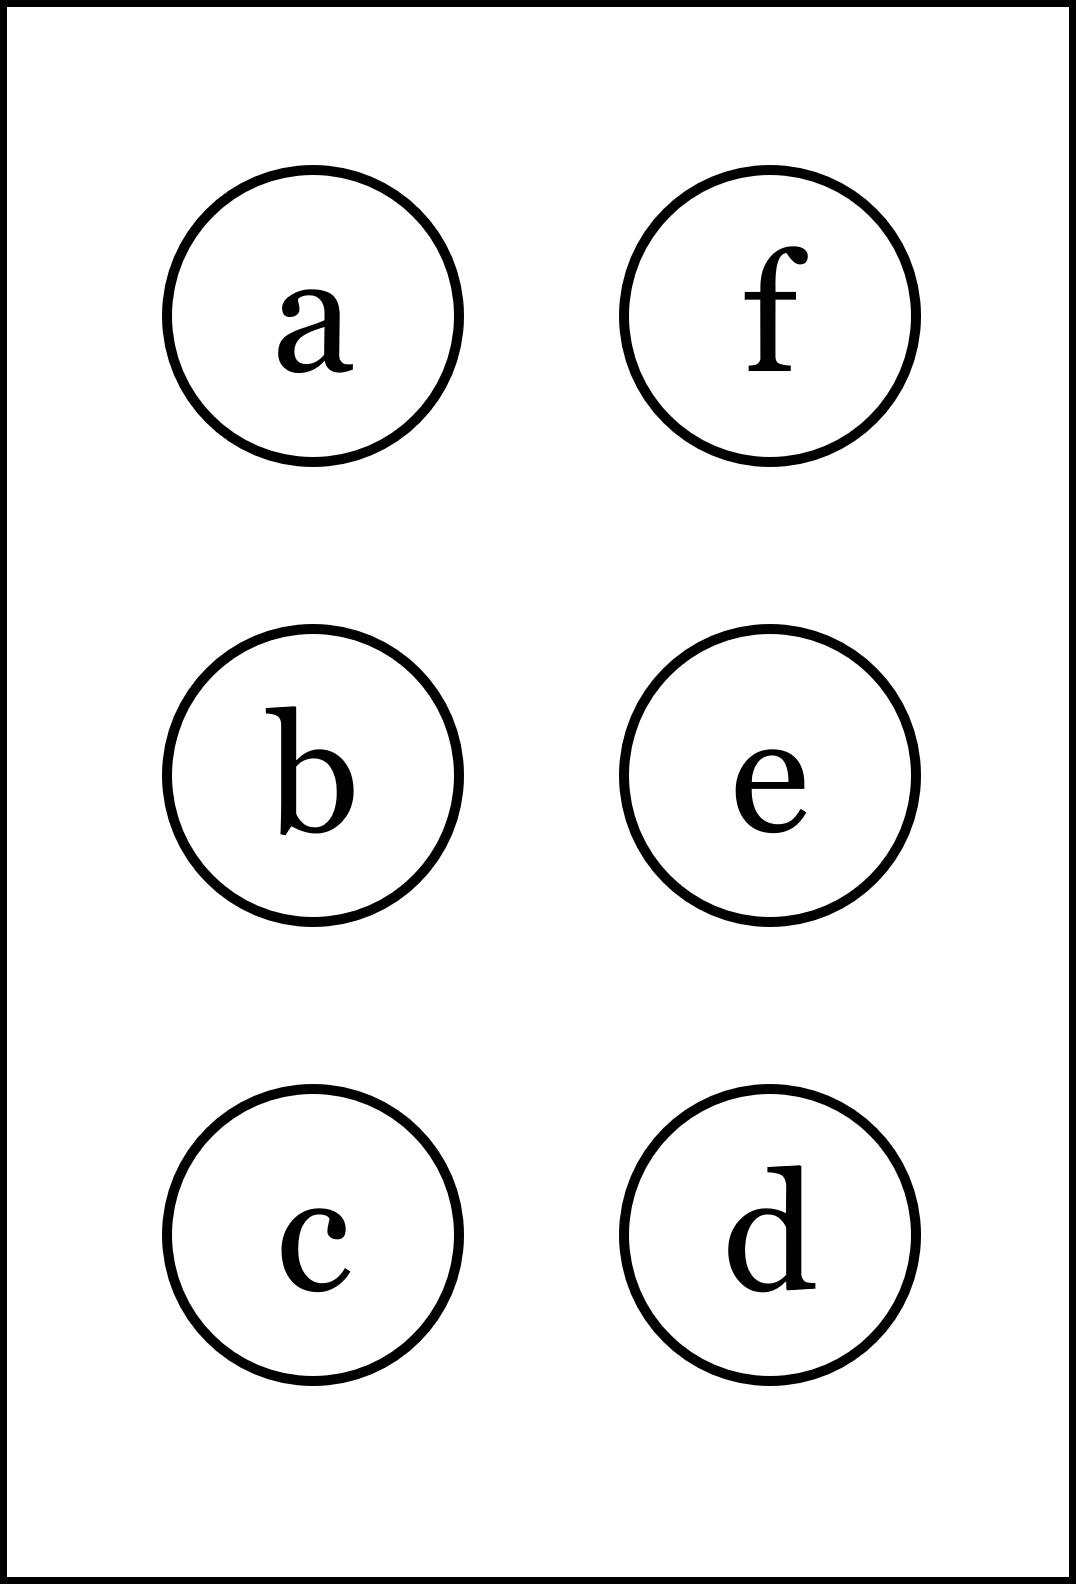
\includegraphics[height=40mm]{../images/braille.png}
{\small Písmeno Braillovej abecedy}
\end{center}
\end{minipage}
\end{center}
\end{minipage}
%
\end{tabular}
\newpage
\thispagestyle{empty}
\begin{tabular}{c:c}
\begin{minipage}[c][104.5mm][t]{0.5\linewidth}
\begin{center}
\vspace{7mm}
{\huge Limity, skupina \textit{Mu $\mu$} -\romannumeral1}\\[5mm]
\textit{Meno:}\phantom{xxxxxxxxxxxxxxxxxxxxxxxxxxxxxxxxxxxxxxxxxxxxxxxxxxxxxxxxxxxxxxxxx}\\[5mm]
\begin{minipage}{0.95\linewidth}
\begin{center}
\textbf{Vypočti limity}. Pokud se výsledky shodujú s tými za otazníky, tak napravo\\obarvi příslušející kroužek načerno. \textbf{Spolu odevzdejte výsledné slovo}.
\end{center}
\end{minipage}
\\[1mm]
\begin{minipage}{0.79\linewidth}
\begin{center}
\begin{varwidth}{\linewidth}
\begin{enumerate}
\normalsize
\item $\lim\limits_{n\to\infty}\cfrac{6+4n}{4+3n}$\quad \dotfill\; ???\;\dotfill \quad $\nicefrac{4}{3}$
\item $\lim\limits_{n\to\infty}\cfrac{-9(-2-4n)}{(n+7)^2}$\quad \dotfill\; ???\;\dotfill \quad $0$
\item $\lim\limits_{n\to\infty}\cfrac{(-1+2n)^2}{n^2-n+2}$\quad \dotfill\; ???\;\dotfill \quad $\infty$
\item $\lim\limits_{n\to\infty}\cfrac{3^{n-3}}{3^{n-3}}$\quad \dotfill\; ???\;\dotfill \quad $-\infty$
\item $\lim\limits_{n\to\infty}\cfrac{\left(\frac{1}{3}\right)^n +4}{-n^{-4}}$\quad \dotfill\; ???\;\dotfill \quad $0$
\item $\lim\limits_{n\to\infty}\cfrac{2\cdot 2^{n+1}+4\cdot 3^{n-2}}{6\cdot 3^{n+2}+9\cdot 2^{n+1}}$\quad \dotfill\; ???\;\dotfill \quad $2$
\end{enumerate}
\end{varwidth}
\end{center}
\end{minipage}
\begin{minipage}{0.20\linewidth}
\begin{center}
{\Huge\bfseries 1.} \\[2mm]
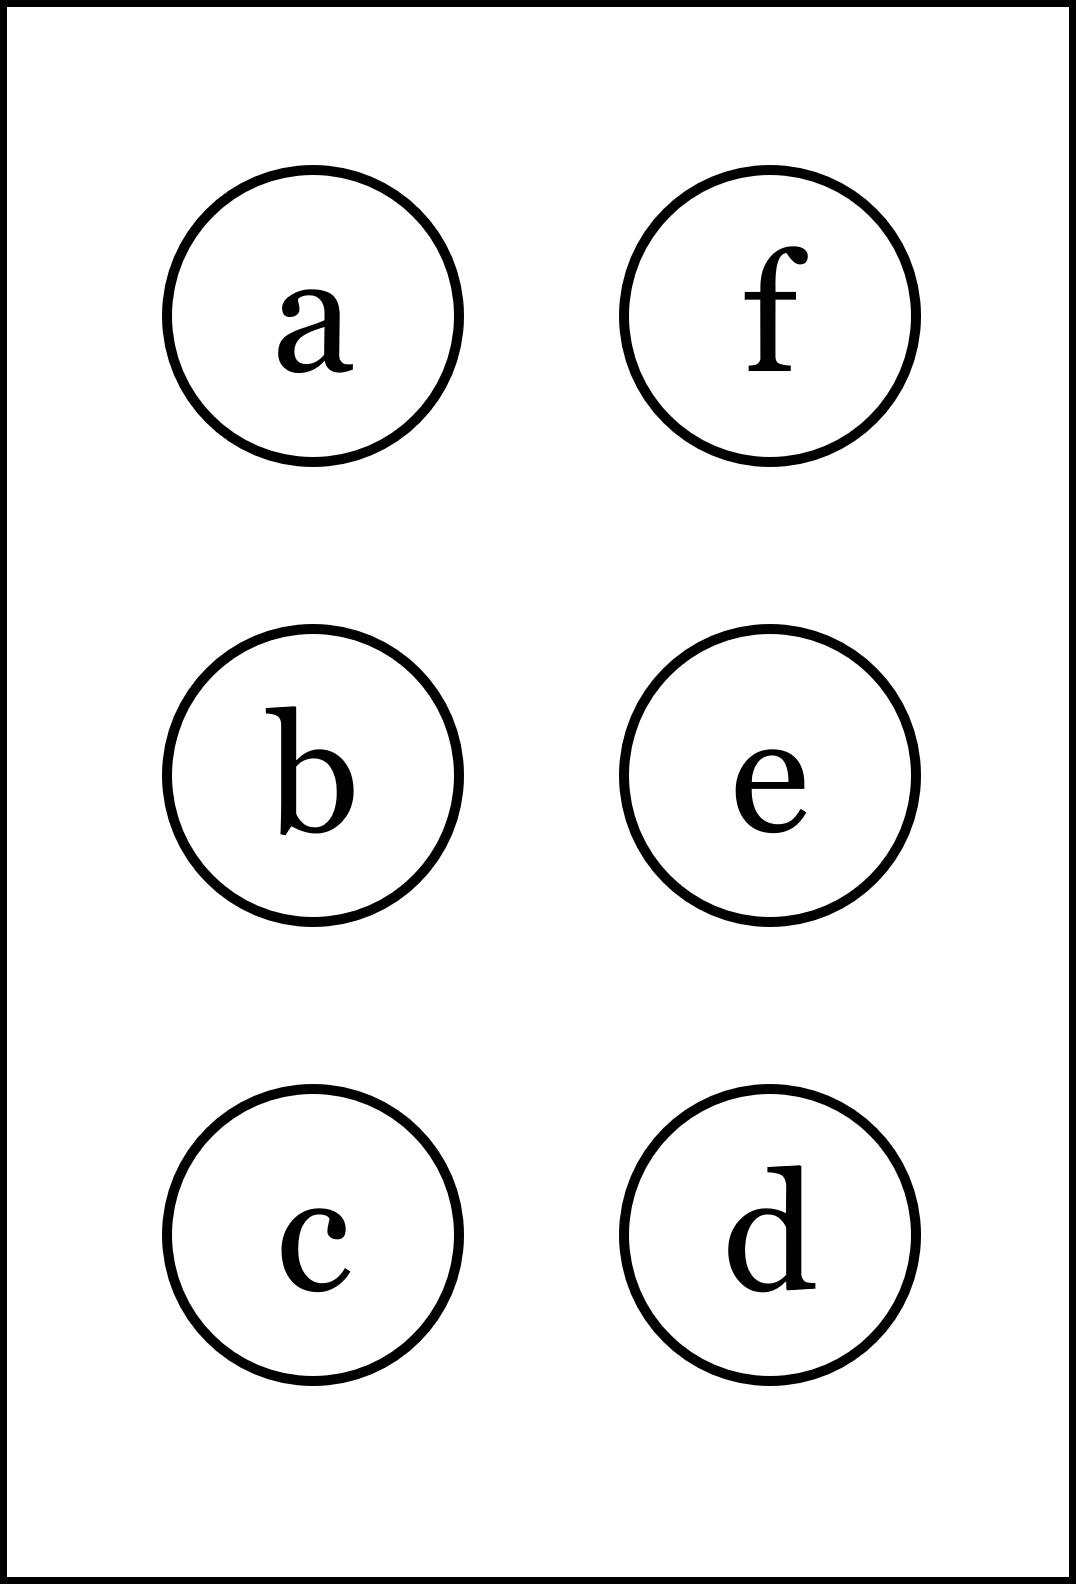
\includegraphics[height=40mm]{../images/braille.png}
{\small Písmeno Braillovej abecedy}
\end{center}
\end{minipage}
\end{center}
\end{minipage}
&
\begin{minipage}[c][104.5mm][t]{0.5\linewidth}
\begin{center}
\vspace{7mm}
{\huge Limity, skupina \textit{Mu $\mu$} -\romannumeral2}\\[5mm]
\textit{Meno:}\phantom{xxxxxxxxxxxxxxxxxxxxxxxxxxxxxxxxxxxxxxxxxxxxxxxxxxxxxxxxxxxxxxxxx}\\[5mm]
\begin{minipage}{0.95\linewidth}
\begin{center}
\textbf{Vypočti limity}. Pokud se výsledky shodujú s tými za otazníky, tak napravo\\obarvi příslušející kroužek načerno. \textbf{Spolu odevzdejte výsledné slovo}.
\end{center}
\end{minipage}
\\[1mm]
\begin{minipage}{0.79\linewidth}
\begin{center}
\begin{varwidth}{\linewidth}
\begin{enumerate}
\normalsize
\item $\lim\limits_{n\to\infty}\cfrac{1-n}{6-9n}$\quad \dotfill\; ???\;\dotfill \quad $\nicefrac{1}{9}$
\item $\lim\limits_{n\to\infty}\cfrac{5(-1+2n)}{(n+6)^2}$\quad \dotfill\; ???\;\dotfill \quad $2$
\item $\lim\limits_{n\to\infty}\cfrac{(-6+n)^2}{n^2-5n-1}$\quad \dotfill\; ???\;\dotfill \quad $1$
\item $\lim\limits_{n\to\infty}\cfrac{4^{n-1}}{4^{n+1}}$\quad \dotfill\; ???\;\dotfill \quad $\infty$
\item $\lim\limits_{n\to\infty}\cfrac{\left(\frac{4}{2}\right)^n +1}{n^{-6}}$\quad \dotfill\; ???\;\dotfill \quad $\infty$
\item $\lim\limits_{n\to\infty}\cfrac{-12\cdot 3^{n+2}-4\cdot 4^{n-2}}{-16\cdot 4^{n+1}+9\cdot 3^{n+2}}$\quad \dotfill\; ???\;\dotfill \quad $1$
\end{enumerate}
\end{varwidth}
\end{center}
\end{minipage}
\begin{minipage}{0.20\linewidth}
\begin{center}
{\Huge\bfseries 2.} \\[2mm]
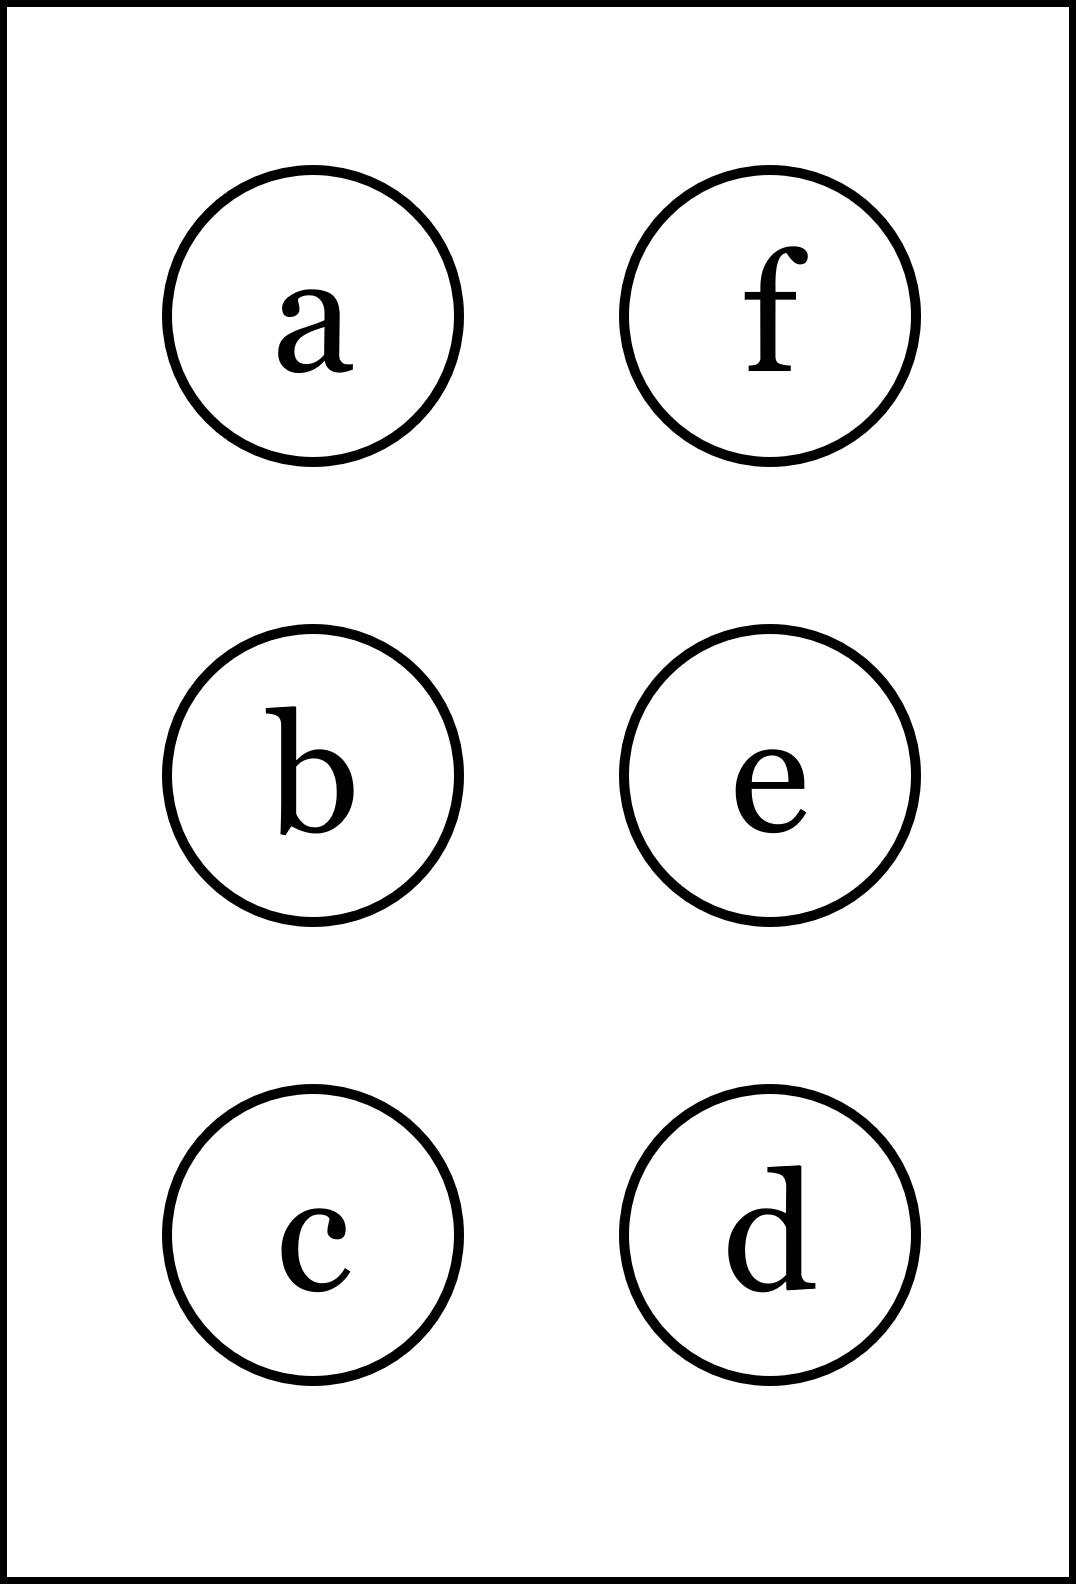
\includegraphics[height=40mm]{../images/braille.png}
{\small Písmeno Braillovej abecedy}
\end{center}
\end{minipage}
\end{center}
\end{minipage}
\\ \hdashline
\begin{minipage}[c][104.5mm][t]{0.5\linewidth}
\begin{center}
\vspace{7mm}
{\huge Limity, skupina \textit{Mu $\mu$} -\romannumeral3}\\[5mm]
\textit{Meno:}\phantom{xxxxxxxxxxxxxxxxxxxxxxxxxxxxxxxxxxxxxxxxxxxxxxxxxxxxxxxxxxxxxxxxx}\\[5mm]
\begin{minipage}{0.95\linewidth}
\begin{center}
\textbf{Vypočti limity}. Pokud se výsledky shodujú s tými za otazníky, tak napravo\\obarvi příslušející kroužek načerno. \textbf{Spolu odevzdejte výsledné slovo}.
\end{center}
\end{minipage}
\\[1mm]
\begin{minipage}{0.79\linewidth}
\begin{center}
\begin{varwidth}{\linewidth}
\begin{enumerate}
\normalsize
\item $\lim\limits_{n\to\infty}\cfrac{3-n}{5+3n}$\quad \dotfill\; ???\;\dotfill \quad $\infty$
\item $\lim\limits_{n\to\infty}\cfrac{1(2-7n)}{(-3n+3)^2}$\quad \dotfill\; ???\;\dotfill \quad $0$
\item $\lim\limits_{n\to\infty}\cfrac{(-6-4n)^2}{n^2-n-1}$\quad \dotfill\; ???\;\dotfill \quad $16$
\item $\lim\limits_{n\to\infty}\cfrac{3^{n+1}}{3^{n+1}}$\quad \dotfill\; ???\;\dotfill \quad $\infty$
\item $\lim\limits_{n\to\infty}\cfrac{\left(\frac{3}{2}\right)^n -2}{-2n^{-12}}$\quad \dotfill\; ???\;\dotfill \quad $-\infty$
\item $\lim\limits_{n\to\infty}\cfrac{12\cdot 3^{n+2}+4\cdot 4^{n+2}}{4\cdot 4^{n-2}+16\cdot 3^{n-2}}$\quad \dotfill\; ???\;\dotfill \quad $256$
\end{enumerate}
\end{varwidth}
\end{center}
\end{minipage}
\begin{minipage}{0.20\linewidth}
\begin{center}
{\Huge\bfseries 3.} \\[2mm]
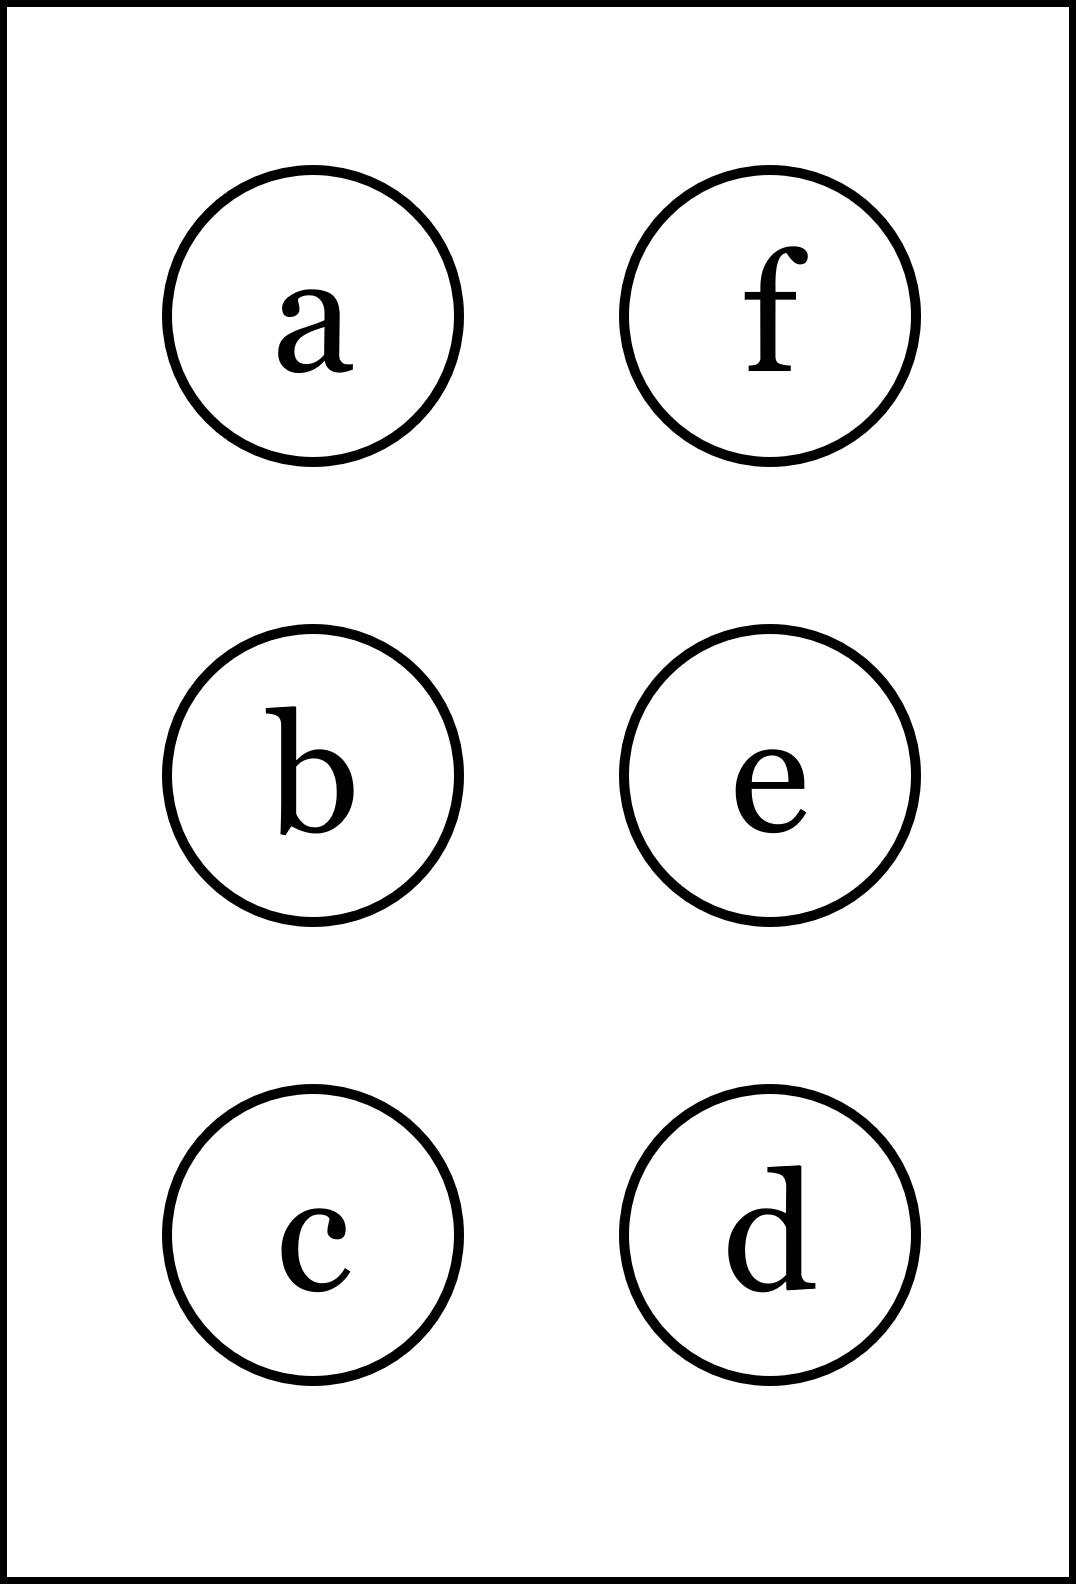
\includegraphics[height=40mm]{../images/braille.png}
{\small Písmeno Braillovej abecedy}
\end{center}
\end{minipage}
\end{center}
\end{minipage}
&
\begin{minipage}[c][104.5mm][t]{0.5\linewidth}
\begin{center}
\vspace{7mm}
{\huge Limity, skupina \textit{Mu $\mu$} -\romannumeral4}\\[5mm]
\textit{Meno:}\phantom{xxxxxxxxxxxxxxxxxxxxxxxxxxxxxxxxxxxxxxxxxxxxxxxxxxxxxxxxxxxxxxxxx}\\[5mm]
\begin{minipage}{0.95\linewidth}
\begin{center}
\textbf{Vypočti limity}. Pokud se výsledky shodujú s tými za otazníky, tak napravo\\obarvi příslušející kroužek načerno. \textbf{Spolu odevzdejte výsledné slovo}.
\end{center}
\end{minipage}
\\[1mm]
\begin{minipage}{0.79\linewidth}
\begin{center}
\begin{varwidth}{\linewidth}
\begin{enumerate}
\normalsize
\item $\lim\limits_{n\to\infty}\cfrac{-1-7n}{-2-n}$\quad \dotfill\; ???\;\dotfill \quad $7$
\item $\lim\limits_{n\to\infty}\cfrac{3(-3+2n)}{(-2n-3)^2}$\quad \dotfill\; ???\;\dotfill \quad $\infty$
\item $\lim\limits_{n\to\infty}\cfrac{(2-4n)^2}{n^2+3n-4}$\quad \dotfill\; ???\;\dotfill \quad $\nicefrac{-4}{3}$
\item $\lim\limits_{n\to\infty}\cfrac{3^{n-1}}{3^{n-3}}$\quad \dotfill\; ???\;\dotfill \quad $-\infty$
\item $\lim\limits_{n\to\infty}\cfrac{\left(\frac{3}{4}\right)^n +2}{-2n^{-9}}$\quad \dotfill\; ???\;\dotfill \quad $-1$
\item $\lim\limits_{n\to\infty}\cfrac{-4\cdot 2^{n-1}-6\cdot 3^{n-2}}{9\cdot 3^{n-1}-3\cdot 2^{n-1}}$\quad \dotfill\; ???\;\dotfill \quad $-2$
\end{enumerate}
\end{varwidth}
\end{center}
\end{minipage}
\begin{minipage}{0.20\linewidth}
\begin{center}
{\Huge\bfseries 4.} \\[2mm]
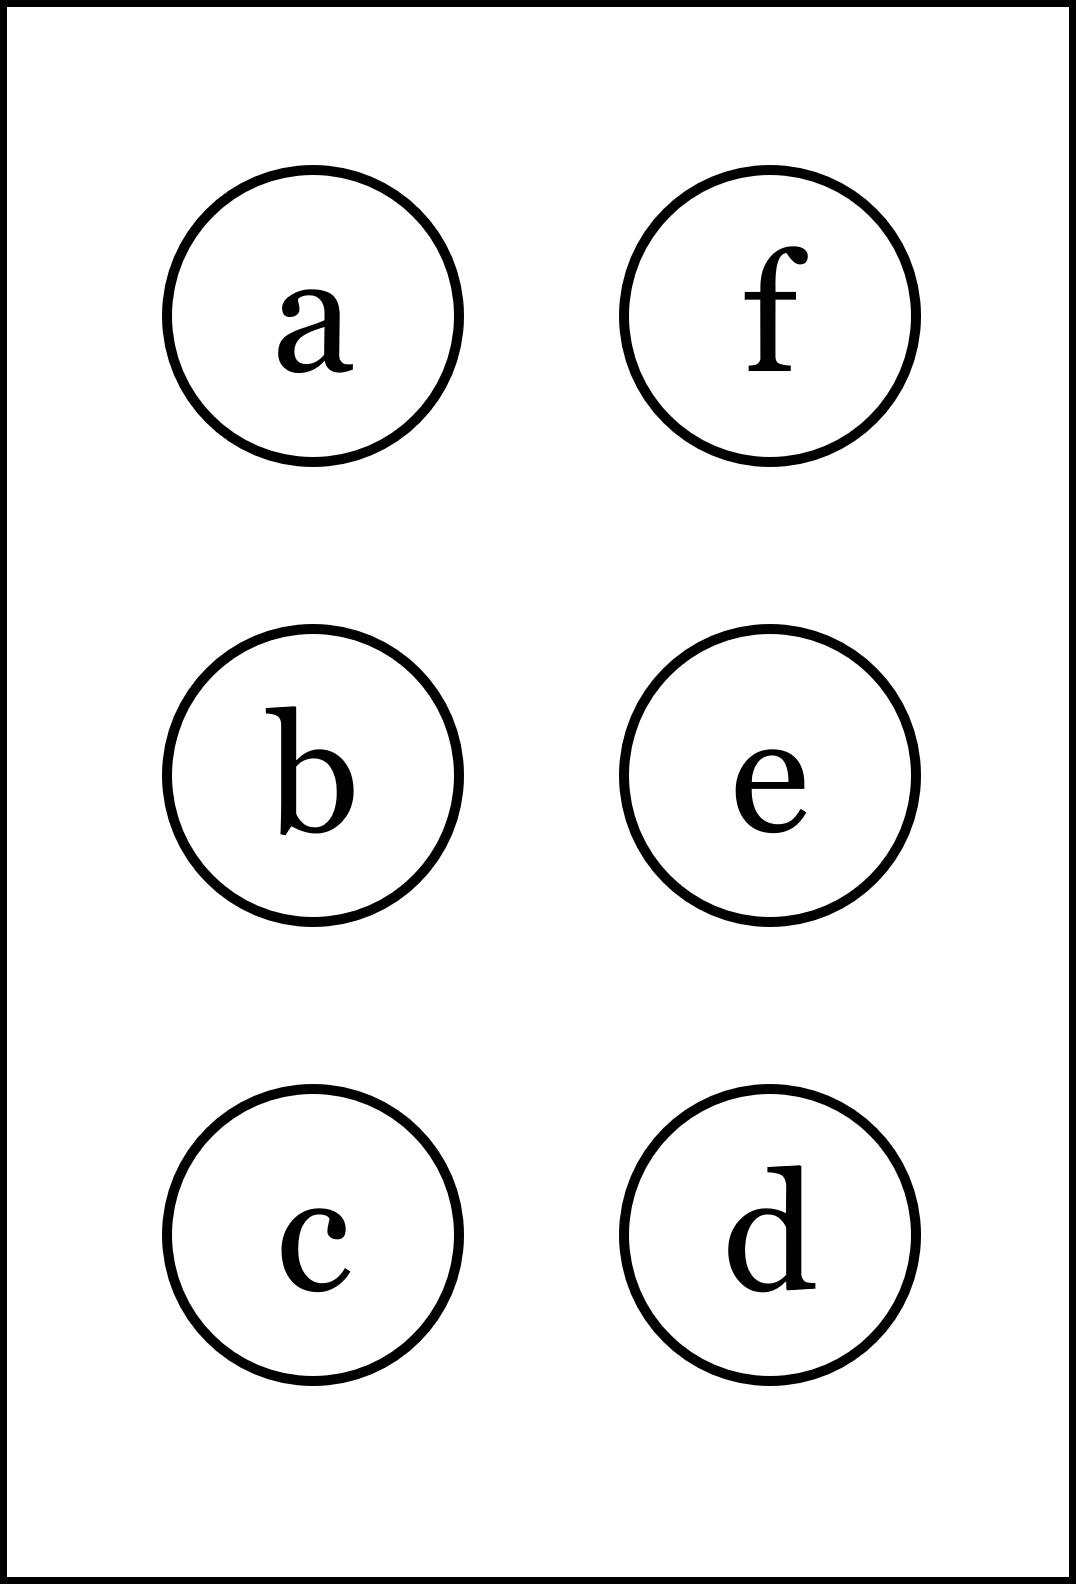
\includegraphics[height=40mm]{../images/braille.png}
{\small Písmeno Braillovej abecedy}
\end{center}
\end{minipage}
\end{center}
\end{minipage}
%
\end{tabular}
\newpage
\thispagestyle{empty}
\begin{tabular}{c:c}
\begin{minipage}[c][104.5mm][t]{0.5\linewidth}
\begin{center}
\vspace{7mm}
{\huge Limity, skupina \textit{Nu $\nu$} -\romannumeral1}\\[5mm]
\textit{Meno:}\phantom{xxxxxxxxxxxxxxxxxxxxxxxxxxxxxxxxxxxxxxxxxxxxxxxxxxxxxxxxxxxxxxxxx}\\[5mm]
\begin{minipage}{0.95\linewidth}
\begin{center}
\textbf{Vypočti limity}. Pokud se výsledky shodujú s tými za otazníky, tak napravo\\obarvi příslušející kroužek načerno. \textbf{Spolu odevzdejte výsledné slovo}.
\end{center}
\end{minipage}
\\[1mm]
\begin{minipage}{0.79\linewidth}
\begin{center}
\begin{varwidth}{\linewidth}
\begin{enumerate}
\normalsize
\item $\lim\limits_{n\to\infty}\cfrac{5+6n}{2-2n}$\quad \dotfill\; ???\;\dotfill \quad $-3$
\item $\lim\limits_{n\to\infty}\cfrac{3(-5-4n)}{(n-5)^2}$\quad \dotfill\; ???\;\dotfill \quad $0$
\item $\lim\limits_{n\to\infty}\cfrac{(-2+3n)^2}{n^2+5n-2}$\quad \dotfill\; ???\;\dotfill \quad $9$
\item $\lim\limits_{n\to\infty}\cfrac{2^{n+3}}{2^{n+1}}$\quad \dotfill\; ???\;\dotfill \quad $4$
\item $\lim\limits_{n\to\infty}\cfrac{\left(\frac{1}{2}\right)^n +4}{2n^{-4}}$\quad \dotfill\; ???\;\dotfill \quad $-\infty$
\item $\lim\limits_{n\to\infty}\cfrac{4\cdot 2^{n+2}+6\cdot 3^{n-2}}{6\cdot 3^{n+2}+2\cdot 2^{n+1}}$\quad \dotfill\; ???\;\dotfill \quad $3$
\end{enumerate}
\end{varwidth}
\end{center}
\end{minipage}
\begin{minipage}{0.20\linewidth}
\begin{center}
{\Huge\bfseries 1.} \\[2mm]
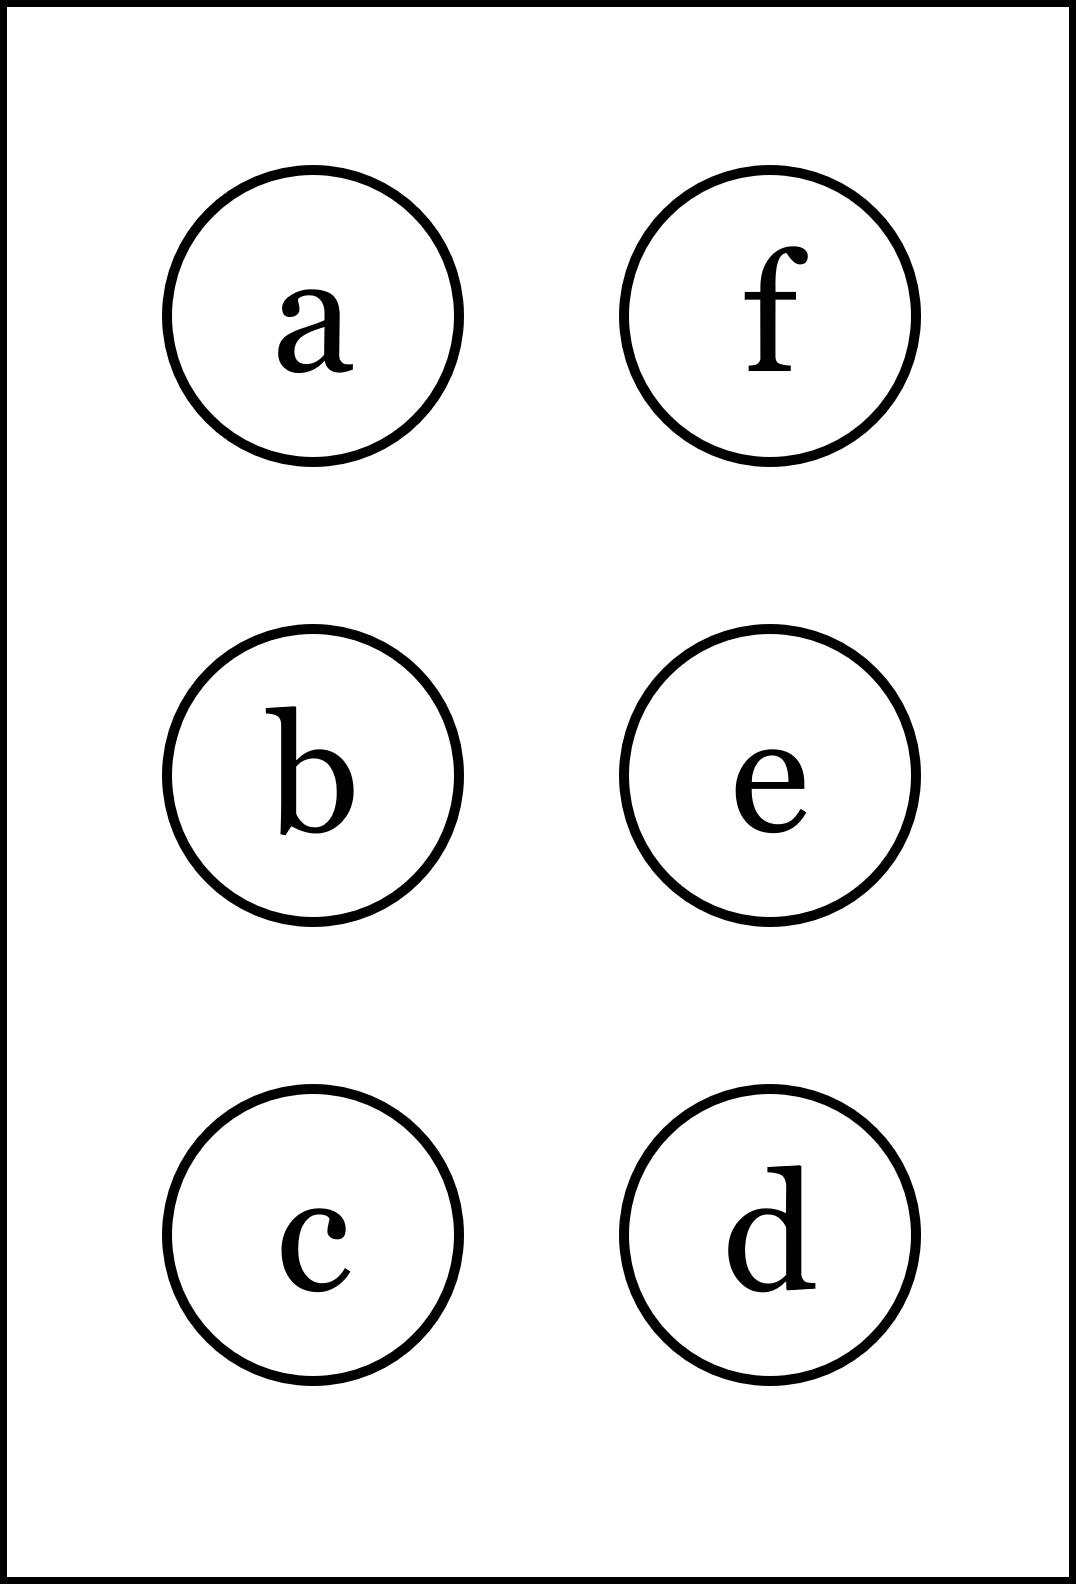
\includegraphics[height=40mm]{../images/braille.png}
{\small Písmeno Braillovej abecedy}
\end{center}
\end{minipage}
\end{center}
\end{minipage}
&
\begin{minipage}[c][104.5mm][t]{0.5\linewidth}
\begin{center}
\vspace{7mm}
{\huge Limity, skupina \textit{Nu $\nu$} -\romannumeral2}\\[5mm]
\textit{Meno:}\phantom{xxxxxxxxxxxxxxxxxxxxxxxxxxxxxxxxxxxxxxxxxxxxxxxxxxxxxxxxxxxxxxxxx}\\[5mm]
\begin{minipage}{0.95\linewidth}
\begin{center}
\textbf{Vypočti limity}. Pokud se výsledky shodujú s tými za otazníky, tak napravo\\obarvi příslušející kroužek načerno. \textbf{Spolu odevzdejte výsledné slovo}.
\end{center}
\end{minipage}
\\[1mm]
\begin{minipage}{0.79\linewidth}
\begin{center}
\begin{varwidth}{\linewidth}
\begin{enumerate}
\normalsize
\item $\lim\limits_{n\to\infty}\cfrac{-4-4n}{2+7n}$\quad \dotfill\; ???\;\dotfill \quad $\nicefrac{-4}{7}$
\item $\lim\limits_{n\to\infty}\cfrac{3(-4-2n)}{(-n+2)^2}$\quad \dotfill\; ???\;\dotfill \quad 3
\item $\lim\limits_{n\to\infty}\cfrac{(-3+n)^2}{n^2+5n+4}$\quad \dotfill\; ???\;\dotfill \quad $\infty$
\item $\lim\limits_{n\to\infty}\cfrac{2^{n+1}}{2^{n-2}}$\quad \dotfill\; ???\;\dotfill \quad $\infty$
\item $\lim\limits_{n\to\infty}\cfrac{\left(\frac{2}{3}\right)^n -4}{n^{-6}}$\quad \dotfill\; ???\;\dotfill \quad $0$
\item $\lim\limits_{n\to\infty}\cfrac{-4\cdot 2^{n-1}+4\cdot 4^{n-1}}{2\cdot 4^{n+2}-4\cdot 2^{n+2}}$\quad \dotfill\; ???\;\dotfill \quad $8$
\end{enumerate}
\end{varwidth}
\end{center}
\end{minipage}
\begin{minipage}{0.20\linewidth}
\begin{center}
{\Huge\bfseries 2.} \\[2mm]
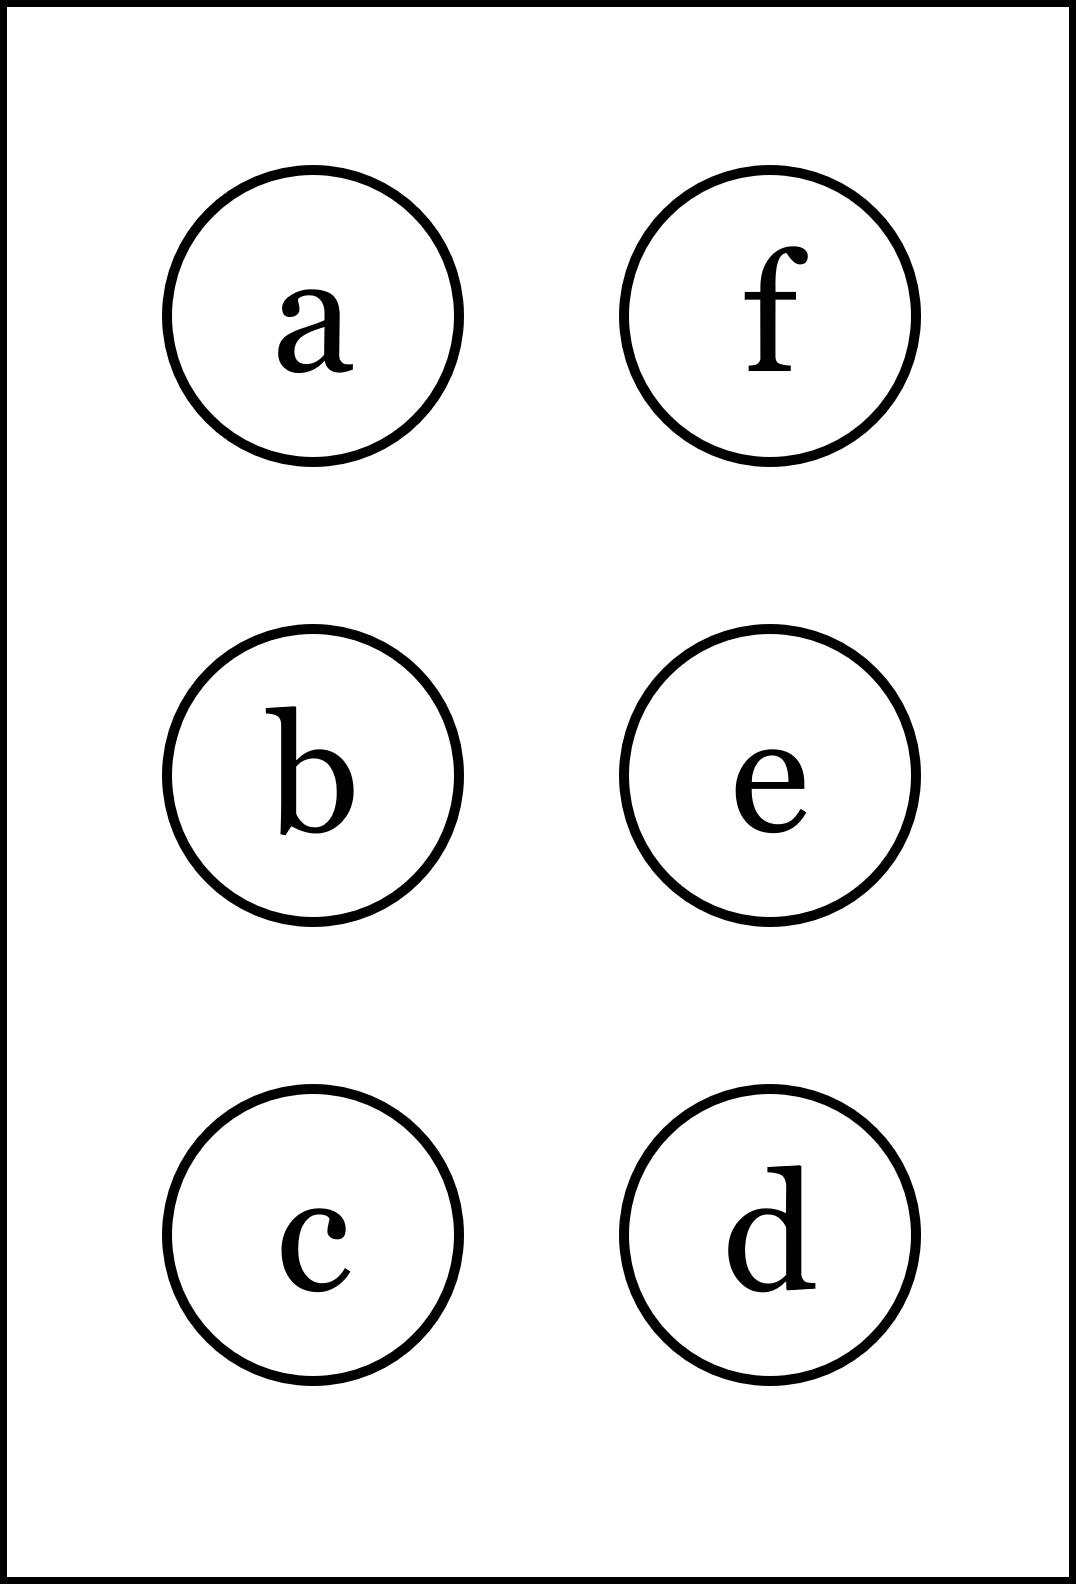
\includegraphics[height=40mm]{../images/braille.png}
{\small Písmeno Braillovej abecedy}
\end{center}
\end{minipage}
\end{center}
\end{minipage}
\\ \hdashline
\begin{minipage}[c][104.5mm][t]{0.5\linewidth}
\begin{center}
\vspace{7mm}
{\huge Limity, skupina \textit{Nu $\nu$} -\romannumeral3}\\[5mm]
\textit{Meno:}\phantom{xxxxxxxxxxxxxxxxxxxxxxxxxxxxxxxxxxxxxxxxxxxxxxxxxxxxxxxxxxxxxxxxx}\\[5mm]
\begin{minipage}{0.95\linewidth}
\begin{center}
\textbf{Vypočti limity}. Pokud se výsledky shodujú s tými za otazníky, tak napravo\\obarvi příslušející kroužek načerno. \textbf{Spolu odevzdejte výsledné slovo}.
\end{center}
\end{minipage}
\\[1mm]
\begin{minipage}{0.79\linewidth}
\begin{center}
\begin{varwidth}{\linewidth}
\begin{enumerate}
\normalsize
\item $\lim\limits_{n\to\infty}\cfrac{-1-6n}{4-n}$\quad \dotfill\; ???\;\dotfill \quad $6$
\item $\lim\limits_{n\to\infty}\cfrac{-2(7+n)}{(-8n-5)^2}$\quad \dotfill\; ???\;\dotfill \quad -2
\item $\lim\limits_{n\to\infty}\cfrac{(-3+n)^2}{n^2+5n-3}$\quad \dotfill\; ???\;\dotfill \quad $1$
\item $\lim\limits_{n\to\infty}\cfrac{2^{n+2}}{2^{n-1}}$\quad \dotfill\; ???\;\dotfill \quad $0$
\item $\lim\limits_{n\to\infty}\cfrac{\left(\frac{2}{3}\right)^n +4}{n^{9}}$\quad \dotfill\; ???\;\dotfill \quad $0$
\item $\lim\limits_{n\to\infty}\cfrac{-8\cdot 2^{n-2}-4\cdot 4^{n+2}}{16\cdot 4^{n-2}-2\cdot 2^{n-1}}$\quad \dotfill\; ???\;\dotfill \quad $-64$
\end{enumerate}
\end{varwidth}
\end{center}
\end{minipage}
\begin{minipage}{0.20\linewidth}
\begin{center}
{\Huge\bfseries 3.} \\[2mm]
\includegraphics[height=40mm]{../images/braille.png}
{\small Písmeno Braillovej abecedy}
\end{center}
\end{minipage}
\end{center}
\end{minipage}
&
\begin{minipage}[c][104.5mm][t]{0.5\linewidth}
\begin{center}
\vspace{7mm}
{\huge Limity, skupina \textit{Nu $\nu$} -\romannumeral4}\\[5mm]
\textit{Meno:}\phantom{xxxxxxxxxxxxxxxxxxxxxxxxxxxxxxxxxxxxxxxxxxxxxxxxxxxxxxxxxxxxxxxxx}\\[5mm]
\begin{minipage}{0.95\linewidth}
\begin{center}
\textbf{Vypočti limity}. Pokud se výsledky shodujú s tými za otazníky, tak napravo\\obarvi příslušející kroužek načerno. \textbf{Spolu odevzdejte výsledné slovo}.
\end{center}
\end{minipage}
\\[1mm]
\begin{minipage}{0.79\linewidth}
\begin{center}
\begin{varwidth}{\linewidth}
\begin{enumerate}
\normalsize
\item $\lim\limits_{n\to\infty}\cfrac{1+2n}{4+4n}$\quad \dotfill\; ???\;\dotfill \quad $\nicefrac{1}{2}$
\item $\lim\limits_{n\to\infty}\cfrac{-3(-3-3n)}{(-2n+4)^2}$\quad \dotfill\; ???\;\dotfill \quad $\infty$
\item $\lim\limits_{n\to\infty}\cfrac{(-2+2n)^2}{n^2-3n-8}$\quad \dotfill\; ???\;\dotfill \quad $-\infty$
\item $\lim\limits_{n\to\infty}\cfrac{3^{n-2}}{3^{n-3}}$\quad \dotfill\; ???\;\dotfill \quad $-\infty$
\item $\lim\limits_{n\to\infty}\cfrac{\left(\frac{2}{3}\right)^n +3}{3n^{9}}$\quad \dotfill\; ???\;\dotfill \quad $9$
\item $\lim\limits_{n\to\infty}\cfrac{4\cdot 2^{n-2}-16\cdot 4^{n-1}}{2\cdot 4^{n-2}-4\cdot 2^{n+2}}$\quad \dotfill\; ???\;\dotfill \quad $-2$
\end{enumerate}
\end{varwidth}
\end{center}
\end{minipage}
\begin{minipage}{0.20\linewidth}
\begin{center}
{\Huge\bfseries 4.} \\[2mm]
\includegraphics[height=40mm]{../images/braille.png}
{\small Písmeno Braillovej abecedy}
\end{center}
\end{minipage}
\end{center}
\end{minipage}
%
\end{tabular}
\newpage
\thispagestyle{empty}
\begin{tabular}{c:c}
\begin{minipage}[c][104.5mm][t]{0.5\linewidth}
\begin{center}
\vspace{7mm}
{\huge Limity, skupina \textit{Xi $\xi$} -\romannumeral1}\\[5mm]
\textit{Meno:}\phantom{xxxxxxxxxxxxxxxxxxxxxxxxxxxxxxxxxxxxxxxxxxxxxxxxxxxxxxxxxxxxxxxxx}\\[5mm]
\begin{minipage}{0.95\linewidth}
\begin{center}
\textbf{Vypočti limity}. Pokud se výsledky shodujú s tými za otazníky, tak napravo\\obarvi příslušející kroužek načerno. \textbf{Spolu odevzdejte výsledné slovo}.
\end{center}
\end{minipage}
\\[1mm]
\begin{minipage}{0.79\linewidth}
\begin{center}
\begin{varwidth}{\linewidth}
\begin{enumerate}
\normalsize
\item $\lim\limits_{n\to\infty}\cfrac{2+2n}{2+6n}$\quad \dotfill\; ???\;\dotfill \quad $\nicefrac{1}{3}$
\item $\lim\limits_{n\to\infty}\cfrac{-2(-7-9n)}{(2n-4)^2}$\quad \dotfill\; ???\;\dotfill \quad -2
\item $\lim\limits_{n\to\infty}\cfrac{(-8-4n)^2}{n^2+5n+4}$\quad \dotfill\; ???\;\dotfill \quad $16$
\item $\lim\limits_{n\to\infty}\cfrac{2^{n+1}}{2^{n+4}}$\quad \dotfill\; ???\;\dotfill \quad $\nicefrac{1}{8}$
\item $\lim\limits_{n\to\infty}\cfrac{\left(\frac{2}{3}\right)^n +1}{-2n^{16}}$\quad \dotfill\; ???\;\dotfill \quad $0$
\item $\lim\limits_{n\to\infty}\cfrac{2\cdot 2^{n+2}-6\cdot 3^{n+1}}{2\cdot 3^{n+1}-2\cdot 2^{n-2}}$\quad \dotfill\; ???\;\dotfill \quad $\nicefrac{-3}{2}$
\end{enumerate}
\end{varwidth}
\end{center}
\end{minipage}
\begin{minipage}{0.20\linewidth}
\begin{center}
{\Huge\bfseries 1.} \\[2mm]
\includegraphics[height=40mm]{../images/braille.png}
{\small Písmeno Braillovej abecedy}
\end{center}
\end{minipage}
\end{center}
\end{minipage}
&
\begin{minipage}[c][104.5mm][t]{0.5\linewidth}
\begin{center}
\vspace{7mm}
{\huge Limity, skupina \textit{Xi $\xi$} -\romannumeral2}\\[5mm]
\textit{Meno:}\phantom{xxxxxxxxxxxxxxxxxxxxxxxxxxxxxxxxxxxxxxxxxxxxxxxxxxxxxxxxxxxxxxxxx}\\[5mm]
\begin{minipage}{0.95\linewidth}
\begin{center}
\textbf{Vypočti limity}. Pokud se výsledky shodujú s tými za otazníky, tak napravo\\obarvi příslušející kroužek načerno. \textbf{Spolu odevzdejte výsledné slovo}.
\end{center}
\end{minipage}
\\[1mm]
\begin{minipage}{0.79\linewidth}
\begin{center}
\begin{varwidth}{\linewidth}
\begin{enumerate}
\normalsize
\item $\lim\limits_{n\to\infty}\cfrac{6-2n}{-2-4n}$\quad \dotfill\; ???\;\dotfill \quad $\nicefrac{1}{2}$
\item $\lim\limits_{n\to\infty}\cfrac{-5(4-3n)}{(4n+9)^2}$\quad \dotfill\; ???\;\dotfill \quad $-\infty$
\item $\lim\limits_{n\to\infty}\cfrac{(-3+5n)^2}{n^2-2n-1}$\quad \dotfill\; ???\;\dotfill \quad $25$
\item $\lim\limits_{n\to\infty}\cfrac{2^{n+3}}{2^{n-1}}$\quad \dotfill\; ???\;\dotfill \quad $16$
\item $\lim\limits_{n\to\infty}\cfrac{\left(\frac{2}{3}\right)^n -3}{3n^{-12}}$\quad \dotfill\; ???\;\dotfill \quad $-1$
\item $\lim\limits_{n\to\infty}\cfrac{2\cdot 2^{n+2}+6\cdot 3^{n+1}}{3\cdot 3^{n+2}-9\cdot 2^{n+1}}$\quad \dotfill\; ???\;\dotfill \quad $6$
\end{enumerate}
\end{varwidth}
\end{center}
\end{minipage}
\begin{minipage}{0.20\linewidth}
\begin{center}
{\Huge\bfseries 2.} \\[2mm]
\includegraphics[height=40mm]{../images/braille.png}
{\small Písmeno Braillovej abecedy}
\end{center}
\end{minipage}
\end{center}
\end{minipage}
\\ \hdashline
\begin{minipage}[c][104.5mm][t]{0.5\linewidth}
\begin{center}
\vspace{7mm}
{\huge Limity, skupina \textit{Xi $\xi$} -\romannumeral3}\\[5mm]
\textit{Meno:}\phantom{xxxxxxxxxxxxxxxxxxxxxxxxxxxxxxxxxxxxxxxxxxxxxxxxxxxxxxxxxxxxxxxxx}\\[5mm]
\begin{minipage}{0.95\linewidth}
\begin{center}
\textbf{Vypočti limity}. Pokud se výsledky shodujú s tými za otazníky, tak napravo\\obarvi příslušející kroužek načerno. \textbf{Spolu odevzdejte výsledné slovo}.
\end{center}
\end{minipage}
\\[1mm]
\begin{minipage}{0.79\linewidth}
\begin{center}
\begin{varwidth}{\linewidth}
\begin{enumerate}
\normalsize
\item $\lim\limits_{n\to\infty}\cfrac{-2+5n}{1-n}$\quad \dotfill\; ???\;\dotfill \quad $-5$
\item $\lim\limits_{n\to\infty}\cfrac{2(3-n)}{(-2n+4)^2}$\quad \dotfill\; ???\;\dotfill \quad $0$
\item $\lim\limits_{n\to\infty}\cfrac{(3-3n)^2}{n^2+n+6}$\quad \dotfill\; ???\;\dotfill \quad $\infty$
\item $\lim\limits_{n\to\infty}\cfrac{2^{n+4}}{2^{n+1}}$\quad \dotfill\; ???\;\dotfill \quad $\nicefrac{1}{8}$
\item $\lim\limits_{n\to\infty}\cfrac{\left(\frac{2}{3}\right)^n +3}{-n^{6}}$\quad \dotfill\; ???\;\dotfill \quad $-\infty$
\item $\lim\limits_{n\to\infty}\cfrac{4\cdot 2^{n-1}+2\cdot 4^{n+1}}{-2\cdot 4^{n+2}+2\cdot 2^{n+2}}$\quad \dotfill\; ???\;\dotfill \quad $-4$
\end{enumerate}
\end{varwidth}
\end{center}
\end{minipage}
\begin{minipage}{0.20\linewidth}
\begin{center}
{\Huge\bfseries 3.} \\[2mm]
\includegraphics[height=40mm]{../images/braille.png}
{\small Písmeno Braillovej abecedy}
\end{center}
\end{minipage}
\end{center}
\end{minipage}
&
\begin{minipage}[c][104.5mm][t]{0.5\linewidth}
\begin{center}
\vspace{7mm}
{\huge Limity, skupina \textit{Xi $\xi$} -\romannumeral4}\\[5mm]
\textit{Meno:}\phantom{xxxxxxxxxxxxxxxxxxxxxxxxxxxxxxxxxxxxxxxxxxxxxxxxxxxxxxxxxxxxxxxxx}\\[5mm]
\begin{minipage}{0.95\linewidth}
\begin{center}
\textbf{Vypočti limity}. Pokud se výsledky shodujú s tými za otazníky, tak napravo\\obarvi příslušející kroužek načerno. \textbf{Spolu odevzdejte výsledné slovo}.
\end{center}
\end{minipage}
\\[1mm]
\begin{minipage}{0.79\linewidth}
\begin{center}
\begin{varwidth}{\linewidth}
\begin{enumerate}
\normalsize
\item $\lim\limits_{n\to\infty}\cfrac{4-5n}{5+7n}$\quad \dotfill\; ???\;\dotfill \quad $\nicefrac{-5}{7}$
\item $\lim\limits_{n\to\infty}\cfrac{-8(-2+5n)}{(4n+8)^2}$\quad \dotfill\; ???\;\dotfill \quad $0$
\item $\lim\limits_{n\to\infty}\cfrac{(6-5n)^2}{n^2-8n+5}$\quad \dotfill\; ???\;\dotfill \quad $25$
\item $\lim\limits_{n\to\infty}\cfrac{3^{n+2}}{3^{n+2}}$\quad \dotfill\; ???\;\dotfill \quad $\infty$
\item $\lim\limits_{n\to\infty}\cfrac{\left(\frac{2}{3}\right)^n -1}{-4n^{12}}$\quad \dotfill\; ???\;\dotfill \quad $0$
\item $\lim\limits_{n\to\infty}\cfrac{4\cdot 2^{n+1}-6\cdot 3^{n-1}}{-4\cdot 3^{n+2}+9\cdot 2^{n+1}}$\quad \dotfill\; ???\;\dotfill \quad $\nicefrac{9}{2}$
\end{enumerate}
\end{varwidth}
\end{center}
\end{minipage}
\begin{minipage}{0.20\linewidth}
\begin{center}
{\Huge\bfseries 4.} \\[2mm]
\includegraphics[height=40mm]{../images/braille.png}
{\small Písmeno Braillovej abecedy}
\end{center}
\end{minipage}
\end{center}
\end{minipage}
%
\end{tabular}
\newpage
\thispagestyle{empty}
\begin{tabular}{c:c}
\begin{minipage}[c][104.5mm][t]{0.5\linewidth}
\begin{center}
\vspace{7mm}
{\huge Limity, skupina \textit{Omicron $\omicron$} -\romannumeral1}\\[5mm]
\textit{Meno:}\phantom{xxxxxxxxxxxxxxxxxxxxxxxxxxxxxxxxxxxxxxxxxxxxxxxxxxxxxxxxxxxxxxxxx}\\[5mm]
\begin{minipage}{0.95\linewidth}
\begin{center}
\textbf{Vypočti limity}. Pokud se výsledky shodujú s tými za otazníky, tak napravo\\obarvi příslušející kroužek načerno. \textbf{Spolu odevzdejte výsledné slovo}.
\end{center}
\end{minipage}
\\[1mm]
\begin{minipage}{0.79\linewidth}
\begin{center}
\begin{varwidth}{\linewidth}
\begin{enumerate}
\normalsize
\item $\lim\limits_{n\to\infty}\cfrac{-8+8n}{4-3n}$\quad \dotfill\; ???\;\dotfill \quad $\nicefrac{-8}{3}$
\item $\lim\limits_{n\to\infty}\cfrac{4(-6-5n)}{(3n+6)^2}$\quad \dotfill\; ???\;\dotfill \quad $-\infty$
\item $\lim\limits_{n\to\infty}\cfrac{(-3+5n)^2}{n^2+n+2}$\quad \dotfill\; ???\;\dotfill \quad $0$
\item $\lim\limits_{n\to\infty}\cfrac{4^{n+1}}{4^{n-2}}$\quad \dotfill\; ???\;\dotfill \quad $4$
\item $\lim\limits_{n\to\infty}\cfrac{\left(\frac{1}{2}\right)^n +3}{2n^{8}}$\quad \dotfill\; ???\;\dotfill \quad $\nicefrac{3}{2}$
\item $\lim\limits_{n\to\infty}\cfrac{9\cdot 2^{n-1}-4\cdot 3^{n-2}}{-9\cdot 3^{n+1}+9\cdot 2^{n-2}}$\quad \dotfill\; ???\;\dotfill \quad $\nicefrac{4}{243}$
\end{enumerate}
\end{varwidth}
\end{center}
\end{minipage}
\begin{minipage}{0.20\linewidth}
\begin{center}
{\Huge\bfseries 1.} \\[2mm]
\includegraphics[height=40mm]{../images/braille.png}
{\small Písmeno Braillovej abecedy}
\end{center}
\end{minipage}
\end{center}
\end{minipage}
&
\begin{minipage}[c][104.5mm][t]{0.5\linewidth}
\begin{center}
\vspace{7mm}
{\huge Limity, skupina \textit{Omicron $\omicron$} -\romannumeral2}\\[5mm]
\textit{Meno:}\phantom{xxxxxxxxxxxxxxxxxxxxxxxxxxxxxxxxxxxxxxxxxxxxxxxxxxxxxxxxxxxxxxxxx}\\[5mm]
\begin{minipage}{0.95\linewidth}
\begin{center}
\textbf{Vypočti limity}. Pokud se výsledky shodujú s tými za otazníky, tak napravo\\obarvi příslušející kroužek načerno. \textbf{Spolu odevzdejte výsledné slovo}.
\end{center}
\end{minipage}
\\[1mm]
\begin{minipage}{0.79\linewidth}
\begin{center}
\begin{varwidth}{\linewidth}
\begin{enumerate}
\normalsize
\item $\lim\limits_{n\to\infty}\cfrac{-4-4n}{-1+5n}$\quad \dotfill\; ???\;\dotfill \quad $\nicefrac{-4}{5}$
\item $\lim\limits_{n\to\infty}\cfrac{1(5+6n)}{(-2n-1)^2}$\quad \dotfill\; ???\;\dotfill \quad $\infty$
\item $\lim\limits_{n\to\infty}\cfrac{(-7-4n)^2}{n^2+n+1}$\quad \dotfill\; ???\;\dotfill \quad $-\infty$
\item $\lim\limits_{n\to\infty}\cfrac{3^{n-1}}{3^{n-4}}$\quad \dotfill\; ???\;\dotfill \quad $\infty$
\item $\lim\limits_{n\to\infty}\cfrac{\left(\frac{2}{4}\right)^n +1}{-4n^{8}}$\quad \dotfill\; ???\;\dotfill \quad $0$
\item $\lim\limits_{n\to\infty}\cfrac{8\cdot 2^{n-1}-4\cdot 4^{n+1}}{4\cdot 4^{n-1}+8\cdot 2^{n-1}}$\quad \dotfill\; ???\;\dotfill \quad $\nicefrac{-1}{4}$
\end{enumerate}
\end{varwidth}
\end{center}
\end{minipage}
\begin{minipage}{0.20\linewidth}
\begin{center}
{\Huge\bfseries 2.} \\[2mm]
\includegraphics[height=40mm]{../images/braille.png}
{\small Písmeno Braillovej abecedy}
\end{center}
\end{minipage}
\end{center}
\end{minipage}
\\ \hdashline
\begin{minipage}[c][104.5mm][t]{0.5\linewidth}
\begin{center}
\vspace{7mm}
{\huge Limity, skupina \textit{Omicron $\omicron$} -\romannumeral3}\\[5mm]
\textit{Meno:}\phantom{xxxxxxxxxxxxxxxxxxxxxxxxxxxxxxxxxxxxxxxxxxxxxxxxxxxxxxxxxxxxxxxxx}\\[5mm]
\begin{minipage}{0.95\linewidth}
\begin{center}
\textbf{Vypočti limity}. Pokud se výsledky shodujú s tými za otazníky, tak napravo\\obarvi příslušející kroužek načerno. \textbf{Spolu odevzdejte výsledné slovo}.
\end{center}
\end{minipage}
\\[1mm]
\begin{minipage}{0.79\linewidth}
\begin{center}
\begin{varwidth}{\linewidth}
\begin{enumerate}
\normalsize
\item $\lim\limits_{n\to\infty}\cfrac{-5-2n}{8+4n}$\quad \dotfill\; ???\;\dotfill \quad $\nicefrac{-1}{2}$
\item $\lim\limits_{n\to\infty}\cfrac{-7(-1+4n)}{(2n+1)^2}$\quad \dotfill\; ???\;\dotfill \quad $-\infty$
\item $\lim\limits_{n\to\infty}\cfrac{(4-2n)^2}{n^2-3n-4}$\quad \dotfill\; ???\;\dotfill \quad $4$
\item $\lim\limits_{n\to\infty}\cfrac{2^{n+3}}{2^{n+2}}$\quad \dotfill\; ???\;\dotfill \quad $-\infty$
\item $\lim\limits_{n\to\infty}\cfrac{\left(\frac{3}{2}\right)^n +2}{n^{4}}$\quad \dotfill\; ???\;\dotfill \quad $\infty$
\item $\lim\limits_{n\to\infty}\cfrac{-9\cdot 2^{n+1}+6\cdot 3^{n-1}}{-6\cdot 3^{n+1}-6\cdot 2^{n-1}}$\quad \dotfill\; ???\;\dotfill \quad $\nicefrac{-1}{9}$
\end{enumerate}
\end{varwidth}
\end{center}
\end{minipage}
\begin{minipage}{0.20\linewidth}
\begin{center}
{\Huge\bfseries 3.} \\[2mm]
\includegraphics[height=40mm]{../images/braille.png}
{\small Písmeno Braillovej abecedy}
\end{center}
\end{minipage}
\end{center}
\end{minipage}
&
\begin{minipage}[c][104.5mm][t]{0.5\linewidth}
\begin{center}
\vspace{7mm}
{\huge Limity, skupina \textit{Omicron $\omicron$} -\romannumeral4}\\[5mm]
\textit{Meno:}\phantom{xxxxxxxxxxxxxxxxxxxxxxxxxxxxxxxxxxxxxxxxxxxxxxxxxxxxxxxxxxxxxxxxx}\\[5mm]
\begin{minipage}{0.95\linewidth}
\begin{center}
\textbf{Vypočti limity}. Pokud se výsledky shodujú s tými za otazníky, tak napravo\\obarvi příslušející kroužek načerno. \textbf{Spolu odevzdejte výsledné slovo}.
\end{center}
\end{minipage}
\\[1mm]
\begin{minipage}{0.79\linewidth}
\begin{center}
\begin{varwidth}{\linewidth}
\begin{enumerate}
\normalsize
\item $\lim\limits_{n\to\infty}\cfrac{-3+7n}{-4+6n}$\quad \dotfill\; ???\;\dotfill \quad $\nicefrac{7}{6}$
\item $\lim\limits_{n\to\infty}\cfrac{-2(3-2n)}{(n-1)^2}$\quad \dotfill\; ???\;\dotfill \quad $-\infty$
\item $\lim\limits_{n\to\infty}\cfrac{(-4+n)^2}{n^2-4n-1}$\quad \dotfill\; ???\;\dotfill \quad $4$
\item $\lim\limits_{n\to\infty}\cfrac{3^{n+2}}{3^{n+1}}$\quad \dotfill\; ???\;\dotfill \quad $\infty$
\item $\lim\limits_{n\to\infty}\cfrac{\left(\frac{2}{4}\right)^n +1}{3n^{-6}}$\quad \dotfill\; ???\;\dotfill \quad $0$
\item $\lim\limits_{n\to\infty}\cfrac{6\cdot 2^{n-2}-2\cdot 3^{n+2}}{-2\cdot 3^{n+2}-3\cdot 2^{n+2}}$\quad \dotfill\; ???\;\dotfill \quad $\nicefrac{1}{2}$
\end{enumerate}
\end{varwidth}
\end{center}
\end{minipage}
\begin{minipage}{0.20\linewidth}
\begin{center}
{\Huge\bfseries 4.} \\[2mm]
\includegraphics[height=40mm]{../images/braille.png}
{\small Písmeno Braillovej abecedy}
\end{center}
\end{minipage}
\end{center}
\end{minipage}
%
\end{tabular}
\newpage
\thispagestyle{empty}
\begin{tabular}{c:c}
\begin{minipage}[c][104.5mm][t]{0.5\linewidth}
\begin{center}
\vspace{7mm}
{\huge Limity, skupina \textit{Pi $\pi$} -\romannumeral1}\\[5mm]
\textit{Meno:}\phantom{xxxxxxxxxxxxxxxxxxxxxxxxxxxxxxxxxxxxxxxxxxxxxxxxxxxxxxxxxxxxxxxxx}\\[5mm]
\begin{minipage}{0.95\linewidth}
\begin{center}
\textbf{Vypočti limity}. Pokud se výsledky shodujú s tými za otazníky, tak napravo\\obarvi příslušející kroužek načerno. \textbf{Spolu odevzdejte výsledné slovo}.
\end{center}
\end{minipage}
\\[1mm]
\begin{minipage}{0.79\linewidth}
\begin{center}
\begin{varwidth}{\linewidth}
\begin{enumerate}
\normalsize
\item $\lim\limits_{n\to\infty}\cfrac{-5-3n}{6-7n}$\quad \dotfill\; ???\;\dotfill \quad $\nicefrac{-5}{6}$
\item $\lim\limits_{n\to\infty}\cfrac{-5(-3+n)}{(8n-6)^2}$\quad \dotfill\; ???\;\dotfill \quad $0$
\item $\lim\limits_{n\to\infty}\cfrac{(2-6n)^2}{n^2-n+6}$\quad \dotfill\; ???\;\dotfill \quad $\infty$
\item $\lim\limits_{n\to\infty}\cfrac{2^{n-1}}{2^{n-3}}$\quad \dotfill\; ???\;\dotfill \quad $0$
\item $\lim\limits_{n\to\infty}\cfrac{\left(\frac{1}{2}\right)^n +1}{3n^{-6}}$\quad \dotfill\; ???\;\dotfill \quad $0$
\item $\lim\limits_{n\to\infty}\cfrac{9\cdot 2^{n-1}+3\cdot 3^{n-1}}{9\cdot 3^{n-2}-6\cdot 2^{n+2}}$\quad \dotfill\; ???\;\dotfill \quad $1$
\end{enumerate}
\end{varwidth}
\end{center}
\end{minipage}
\begin{minipage}{0.20\linewidth}
\begin{center}
{\Huge\bfseries 1.} \\[2mm]
\includegraphics[height=40mm]{../images/braille.png}
{\small Písmeno Braillovej abecedy}
\end{center}
\end{minipage}
\end{center}
\end{minipage}
&
\begin{minipage}[c][104.5mm][t]{0.5\linewidth}
\begin{center}
\vspace{7mm}
{\huge Limity, skupina \textit{Pi $\pi$} -\romannumeral2}\\[5mm]
\textit{Meno:}\phantom{xxxxxxxxxxxxxxxxxxxxxxxxxxxxxxxxxxxxxxxxxxxxxxxxxxxxxxxxxxxxxxxxx}\\[5mm]
\begin{minipage}{0.95\linewidth}
\begin{center}
\textbf{Vypočti limity}. Pokud se výsledky shodujú s tými za otazníky, tak napravo\\obarvi příslušející kroužek načerno. \textbf{Spolu odevzdejte výsledné slovo}.
\end{center}
\end{minipage}
\\[1mm]
\begin{minipage}{0.79\linewidth}
\begin{center}
\begin{varwidth}{\linewidth}
\begin{enumerate}
\normalsize
\item $\lim\limits_{n\to\infty}\cfrac{3-4n}{7+n}$\quad \dotfill\; ???\;\dotfill \quad $-4$
\item $\lim\limits_{n\to\infty}\cfrac{-5(-4-3n)}{(-3n+5)^2}$\quad \dotfill\; ???\;\dotfill \quad $0$
\item $\lim\limits_{n\to\infty}\cfrac{(-7+5n)^2}{n^2-4n+2}$\quad \dotfill\; ???\;\dotfill \quad $\infty$
\item $\lim\limits_{n\to\infty}\cfrac{2^{n-2}}{2^{n+1}}$\quad \dotfill\; ???\;\dotfill \quad $\infty$
\item $\lim\limits_{n\to\infty}\cfrac{\left(\frac{4}{2}\right)^n +1}{-3n^{-9}}$\quad \dotfill\; ???\;\dotfill \quad $-\infty$
\item $\lim\limits_{n\to\infty}\cfrac{-2\cdot 2^{n-1}+2\cdot 3^{n-1}}{-4\cdot 3^{n-2}-4\cdot 2^{n+1}}$\quad \dotfill\; ???\;\dotfill \quad $\nicefrac{-3}{2}$
\end{enumerate}
\end{varwidth}
\end{center}
\end{minipage}
\begin{minipage}{0.20\linewidth}
\begin{center}
{\Huge\bfseries 2.} \\[2mm]
\includegraphics[height=40mm]{../images/braille.png}
{\small Písmeno Braillovej abecedy}
\end{center}
\end{minipage}
\end{center}
\end{minipage}
\\ \hdashline
\begin{minipage}[c][104.5mm][t]{0.5\linewidth}
\begin{center}
\vspace{7mm}
{\huge Limity, skupina \textit{Pi $\pi$} -\romannumeral3}\\[5mm]
\textit{Meno:}\phantom{xxxxxxxxxxxxxxxxxxxxxxxxxxxxxxxxxxxxxxxxxxxxxxxxxxxxxxxxxxxxxxxxx}\\[5mm]
\begin{minipage}{0.95\linewidth}
\begin{center}
\textbf{Vypočti limity}. Pokud se výsledky shodujú s tými za otazníky, tak napravo\\obarvi příslušející kroužek načerno. \textbf{Spolu odevzdejte výsledné slovo}.
\end{center}
\end{minipage}
\\[1mm]
\begin{minipage}{0.79\linewidth}
\begin{center}
\begin{varwidth}{\linewidth}
\begin{enumerate}
\normalsize
\item $\lim\limits_{n\to\infty}\cfrac{-9+n}{-5-9n}$\quad \dotfill\; ???\;\dotfill \quad $\nicefrac{-1}{9}$
\item $\lim\limits_{n\to\infty}\cfrac{-2(-3-3n)}{(-2n+8)^2}$\quad \dotfill\; ???\;\dotfill \quad $0$
\item $\lim\limits_{n\to\infty}\cfrac{(1-n)^2}{n^2+2n+1}$\quad \dotfill\; ???\;\dotfill \quad $1$
\item $\lim\limits_{n\to\infty}\cfrac{4^{n+2}}{4^{n-2}}$\quad \dotfill\; ???\;\dotfill \quad $-\infty$
\item $\lim\limits_{n\to\infty}\cfrac{\left(\frac{3}{2}\right)^n +3}{-n^{8}}$\quad \dotfill\; ???\;\dotfill \quad $0$
\item $\lim\limits_{n\to\infty}\cfrac{6\cdot 2^{n+2}+3\cdot 3^{n-1}}{3\cdot 3^{n+1}-9\cdot 2^{n-1}}$\quad \dotfill\; ???\;\dotfill \quad $3$
\end{enumerate}
\end{varwidth}
\end{center}
\end{minipage}
\begin{minipage}{0.20\linewidth}
\begin{center}
{\Huge\bfseries 3.} \\[2mm]
\includegraphics[height=40mm]{../images/braille.png}
{\small Písmeno Braillovej abecedy}
\end{center}
\end{minipage}
\end{center}
\end{minipage}
&
\begin{minipage}[c][104.5mm][t]{0.5\linewidth}
\begin{center}
\vspace{7mm}
{\huge Limity, skupina \textit{Pi $\pi$} -\romannumeral4}\\[5mm]
\textit{Meno:}\phantom{xxxxxxxxxxxxxxxxxxxxxxxxxxxxxxxxxxxxxxxxxxxxxxxxxxxxxxxxxxxxxxxxx}\\[5mm]
\begin{minipage}{0.95\linewidth}
\begin{center}
\textbf{Vypočti limity}. Pokud se výsledky shodujú s tými za otazníky, tak napravo\\obarvi příslušející kroužek načerno. \textbf{Spolu odevzdejte výsledné slovo}.
\end{center}
\end{minipage}
\\[1mm]
\begin{minipage}{0.79\linewidth}
\begin{center}
\begin{varwidth}{\linewidth}
\begin{enumerate}
\normalsize
\item $\lim\limits_{n\to\infty}\cfrac{-9-8n}{3+n}$\quad \dotfill\; ???\;\dotfill \quad $-8$
\item $\lim\limits_{n\to\infty}\cfrac{1(1-n)}{(-3n+4)^2}$\quad \dotfill\; ???\;\dotfill \quad $\infty$
\item $\lim\limits_{n\to\infty}\cfrac{(3-6n)^2}{n^2+4n-8}$\quad \dotfill\; ???\;\dotfill \quad $36$
\item $\lim\limits_{n\to\infty}\cfrac{2^{n-1}}{2^{n-4}}$\quad \dotfill\; ???\;\dotfill \quad $8$
\item $\lim\limits_{n\to\infty}\cfrac{\left(\frac{1}{2}\right)^n -3}{4n^{-4}}$\quad \dotfill\; ???\;\dotfill \quad $0$
\item $\lim\limits_{n\to\infty}\cfrac{-3\cdot 2^{n+2}+4\cdot 3^{n+2}}{-3\cdot 3^{n+1}-2\cdot 2^{n-1}}$\quad \dotfill\; ???\;\dotfill \quad $\nicefrac{-4}{9}$
\end{enumerate}
\end{varwidth}
\end{center}
\end{minipage}
\begin{minipage}{0.20\linewidth}
\begin{center}
{\Huge\bfseries 4.} \\[2mm]
\includegraphics[height=40mm]{../images/braille.png}
{\small Písmeno Braillovej abecedy}
\end{center}
\end{minipage}
\end{center}
\end{minipage}
%
\end{tabular}
\newpage
\thispagestyle{empty}
\begin{tabular}{c:c}
\begin{minipage}[c][104.5mm][t]{0.5\linewidth}
\begin{center}
\vspace{7mm}
{\huge Limity, skupina \textit{Rho $\rho$} -\romannumeral1}\\[5mm]
\textit{Meno:}\phantom{xxxxxxxxxxxxxxxxxxxxxxxxxxxxxxxxxxxxxxxxxxxxxxxxxxxxxxxxxxxxxxxxx}\\[5mm]
\begin{minipage}{0.95\linewidth}
\begin{center}
\textbf{Vypočti limity}. Pokud se výsledky shodujú s tými za otazníky, tak napravo\\obarvi příslušející kroužek načerno. \textbf{Spolu odevzdejte výsledné slovo}.
\end{center}
\end{minipage}
\\[1mm]
\begin{minipage}{0.79\linewidth}
\begin{center}
\begin{varwidth}{\linewidth}
\begin{enumerate}
\normalsize
\item $\lim\limits_{n\to\infty}\cfrac{-6+n}{-7-2n}$\quad \dotfill\; ???\;\dotfill \quad $\nicefrac{-1}{2}$
\item $\lim\limits_{n\to\infty}\cfrac{-1(-4+4n)}{(-n+3)^2}$\quad \dotfill\; ???\;\dotfill \quad $0$
\item $\lim\limits_{n\to\infty}\cfrac{(-4+6n)^2}{n^2-3n+6}$\quad \dotfill\; ???\;\dotfill \quad $0$
\item $\lim\limits_{n\to\infty}\cfrac{3^{n-2}}{3^{n+1}}$\quad \dotfill\; ???\;\dotfill \quad $\infty$
\item $\lim\limits_{n\to\infty}\cfrac{\left(\frac{4}{3}\right)^n -2}{2n^{-8}}$\quad \dotfill\; ???\;\dotfill \quad $-8$
\item $\lim\limits_{n\to\infty}\cfrac{-2\cdot 2^{n-1}-16\cdot 4^{n-1}}{8\cdot 4^{n+1}-8\cdot 2^{n+1}}$\quad \dotfill\; ???\;\dotfill \quad $-8$
\end{enumerate}
\end{varwidth}
\end{center}
\end{minipage}
\begin{minipage}{0.20\linewidth}
\begin{center}
{\Huge\bfseries 1.} \\[2mm]
\includegraphics[height=40mm]{../images/braille.png}
{\small Písmeno Braillovej abecedy}
\end{center}
\end{minipage}
\end{center}
\end{minipage}
&
\begin{minipage}[c][104.5mm][t]{0.5\linewidth}
\begin{center}
\vspace{7mm}
{\huge Limity, skupina \textit{Rho $\rho$} -\romannumeral2}\\[5mm]
\textit{Meno:}\phantom{xxxxxxxxxxxxxxxxxxxxxxxxxxxxxxxxxxxxxxxxxxxxxxxxxxxxxxxxxxxxxxxxx}\\[5mm]
\begin{minipage}{0.95\linewidth}
\begin{center}
\textbf{Vypočti limity}. Pokud se výsledky shodujú s tými za otazníky, tak napravo\\obarvi příslušející kroužek načerno. \textbf{Spolu odevzdejte výsledné slovo}.
\end{center}
\end{minipage}
\\[1mm]
\begin{minipage}{0.79\linewidth}
\begin{center}
\begin{varwidth}{\linewidth}
\begin{enumerate}
\normalsize
\item $\lim\limits_{n\to\infty}\cfrac{2-4n}{-7-6n}$\quad \dotfill\; ???\;\dotfill \quad $\nicefrac{2}{3}$
\item $\lim\limits_{n\to\infty}\cfrac{-4(3+3n)}{(-5n-2)^2}$\quad \dotfill\; ???\;\dotfill \quad $\nicefrac{3}{20}$
\item $\lim\limits_{n\to\infty}\cfrac{(3-n)^2}{n^2+4n-7}$\quad \dotfill\; ???\;\dotfill \quad $\nicefrac{-1}{4}$
\item $\lim\limits_{n\to\infty}\cfrac{3^{n+3}}{3^{n-1}}$\quad \dotfill\; ???\;\dotfill \quad $81$
\item $\lim\limits_{n\to\infty}\cfrac{\left(\frac{1}{2}\right)^n -1}{-n^{9}}$\quad \dotfill\; ???\;\dotfill \quad $-\infty$
\item $\lim\limits_{n\to\infty}\cfrac{16\cdot 3^{n-2}-4\cdot 4^{n-1}}{12\cdot 4^{n-1}-3\cdot 3^{n+2}}$\quad \dotfill\; ???\;\dotfill \quad $\nicefrac{-1}{9}$
\end{enumerate}
\end{varwidth}
\end{center}
\end{minipage}
\begin{minipage}{0.20\linewidth}
\begin{center}
{\Huge\bfseries 2.} \\[2mm]
\includegraphics[height=40mm]{../images/braille.png}
{\small Písmeno Braillovej abecedy}
\end{center}
\end{minipage}
\end{center}
\end{minipage}
\\ \hdashline
\begin{minipage}[c][104.5mm][t]{0.5\linewidth}
\begin{center}
\vspace{7mm}
{\huge Limity, skupina \textit{Rho $\rho$} -\romannumeral3}\\[5mm]
\textit{Meno:}\phantom{xxxxxxxxxxxxxxxxxxxxxxxxxxxxxxxxxxxxxxxxxxxxxxxxxxxxxxxxxxxxxxxxx}\\[5mm]
\begin{minipage}{0.95\linewidth}
\begin{center}
\textbf{Vypočti limity}. Pokud se výsledky shodujú s tými za otazníky, tak napravo\\obarvi příslušející kroužek načerno. \textbf{Spolu odevzdejte výsledné slovo}.
\end{center}
\end{minipage}
\\[1mm]
\begin{minipage}{0.79\linewidth}
\begin{center}
\begin{varwidth}{\linewidth}
\begin{enumerate}
\normalsize
\item $\lim\limits_{n\to\infty}\cfrac{-1-2n}{8+2n}$\quad \dotfill\; ???\;\dotfill \quad $-1$
\item $\lim\limits_{n\to\infty}\cfrac{-3(9+4n)}{(-4n+2)^2}$\quad \dotfill\; ???\;\dotfill \quad $0$
\item $\lim\limits_{n\to\infty}\cfrac{(9-9n)^2}{n^2+6n+6}$\quad \dotfill\; ???\;\dotfill \quad $0$
\item $\lim\limits_{n\to\infty}\cfrac{4^{n-3}}{4^{n-1}}$\quad \dotfill\; ???\;\dotfill \quad $\infty$
\item $\lim\limits_{n\to\infty}\cfrac{\left(\frac{2}{3}\right)^n -1}{n^{6}}$\quad \dotfill\; ???\;\dotfill \quad $-1$
\item $\lim\limits_{n\to\infty}\cfrac{-6\cdot 2^{n-2}+9\cdot 3^{n-2}}{4\cdot 3^{n+1}+4\cdot 2^{n+1}}$\quad \dotfill\; ???\;\dotfill \quad $\nicefrac{27}{4}$
\end{enumerate}
\end{varwidth}
\end{center}
\end{minipage}
\begin{minipage}{0.20\linewidth}
\begin{center}
{\Huge\bfseries 3.} \\[2mm]
\includegraphics[height=40mm]{../images/braille.png}
{\small Písmeno Braillovej abecedy}
\end{center}
\end{minipage}
\end{center}
\end{minipage}
&
\begin{minipage}[c][104.5mm][t]{0.5\linewidth}
\begin{center}
\vspace{7mm}
{\huge Limity, skupina \textit{Rho $\rho$} -\romannumeral4}\\[5mm]
\textit{Meno:}\phantom{xxxxxxxxxxxxxxxxxxxxxxxxxxxxxxxxxxxxxxxxxxxxxxxxxxxxxxxxxxxxxxxxx}\\[5mm]
\begin{minipage}{0.95\linewidth}
\begin{center}
\textbf{Vypočti limity}. Pokud se výsledky shodujú s tými za otazníky, tak napravo\\obarvi příslušející kroužek načerno. \textbf{Spolu odevzdejte výsledné slovo}.
\end{center}
\end{minipage}
\\[1mm]
\begin{minipage}{0.79\linewidth}
\begin{center}
\begin{varwidth}{\linewidth}
\begin{enumerate}
\normalsize
\item $\lim\limits_{n\to\infty}\cfrac{-1+7n}{4-2n}$\quad \dotfill\; ???\;\dotfill \quad $\nicefrac{-7}{2}$
\item $\lim\limits_{n\to\infty}\cfrac{-3(1+4n)}{(-2n+4)^2}$\quad \dotfill\; ???\;\dotfill \quad $\infty$
\item $\lim\limits_{n\to\infty}\cfrac{(-8+5n)^2}{n^2+2n-1}$\quad \dotfill\; ???\;\dotfill \quad $8$
\item $\lim\limits_{n\to\infty}\cfrac{3^{n-1}}{3^{n-4}}$\quad \dotfill\; ???\;\dotfill \quad $\nicefrac{1}{27}$
\item $\lim\limits_{n\to\infty}\cfrac{\left(\frac{1}{4}\right)^n +1}{-2n^{9}}$\quad \dotfill\; ???\;\dotfill \quad $9$
\item $\lim\limits_{n\to\infty}\cfrac{3\cdot 3^{n-1}+16\cdot 4^{n+2}}{-9\cdot 4^{n-2}-16\cdot 3^{n-1}}$\quad \dotfill\; ???\;\dotfill \quad $\nicefrac{-4}{9}$
\end{enumerate}
\end{varwidth}
\end{center}
\end{minipage}
\begin{minipage}{0.20\linewidth}
\begin{center}
{\Huge\bfseries 4.} \\[2mm]
\includegraphics[height=40mm]{../images/braille.png}
{\small Písmeno Braillovej abecedy}
\end{center}
\end{minipage}
\end{center}
\end{minipage}
%
\end{tabular}
\newpage
\thispagestyle{empty}
\begin{tabular}{c:c}
\begin{minipage}[c][104.5mm][t]{0.5\linewidth}
\begin{center}
\vspace{7mm}
{\huge Limity, skupina \textit{Sigma $\sigma$} -\romannumeral1}\\[5mm]
\textit{Meno:}\phantom{xxxxxxxxxxxxxxxxxxxxxxxxxxxxxxxxxxxxxxxxxxxxxxxxxxxxxxxxxxxxxxxxx}\\[5mm]
\begin{minipage}{0.95\linewidth}
\begin{center}
\textbf{Vypočti limity}. Pokud se výsledky shodujú s tými za otazníky, tak napravo\\obarvi příslušející kroužek načerno. \textbf{Spolu odevzdejte výsledné slovo}.
\end{center}
\end{minipage}
\\[1mm]
\begin{minipage}{0.79\linewidth}
\begin{center}
\begin{varwidth}{\linewidth}
\begin{enumerate}
\normalsize
\item $\lim\limits_{n\to\infty}\cfrac{-1+4n}{-9+3n}$\quad \dotfill\; ???\;\dotfill \quad $\nicefrac{4}{3}$
\item $\lim\limits_{n\to\infty}\cfrac{4(-2-3n)}{(-5n-2)^2}$\quad \dotfill\; ???\;\dotfill \quad 4
\item $\lim\limits_{n\to\infty}\cfrac{(-3+5n)^2}{n^2-6n+7}$\quad \dotfill\; ???\;\dotfill \quad $25$
\item $\lim\limits_{n\to\infty}\cfrac{3^{n+3}}{3^{n+2}}$\quad \dotfill\; ???\;\dotfill \quad $-\infty$
\item $\lim\limits_{n\to\infty}\cfrac{\left(\frac{2}{4}\right)^n -2}{2n^{-12}}$\quad \dotfill\; ???\;\dotfill \quad $0$
\item $\lim\limits_{n\to\infty}\cfrac{8\cdot 2^{n+2}-16\cdot 4^{n+1}}{-16\cdot 4^{n+1}+2\cdot 2^{n-1}}$\quad \dotfill\; ???\;\dotfill \quad $1$
\end{enumerate}
\end{varwidth}
\end{center}
\end{minipage}
\begin{minipage}{0.20\linewidth}
\begin{center}
{\Huge\bfseries 1.} \\[2mm]
\includegraphics[height=40mm]{../images/braille.png}
{\small Písmeno Braillovej abecedy}
\end{center}
\end{minipage}
\end{center}
\end{minipage}
&
\begin{minipage}[c][104.5mm][t]{0.5\linewidth}
\begin{center}
\vspace{7mm}
{\huge Limity, skupina \textit{Sigma $\sigma$} -\romannumeral2}\\[5mm]
\textit{Meno:}\phantom{xxxxxxxxxxxxxxxxxxxxxxxxxxxxxxxxxxxxxxxxxxxxxxxxxxxxxxxxxxxxxxxxx}\\[5mm]
\begin{minipage}{0.95\linewidth}
\begin{center}
\textbf{Vypočti limity}. Pokud se výsledky shodujú s tými za otazníky, tak napravo\\obarvi příslušející kroužek načerno. \textbf{Spolu odevzdejte výsledné slovo}.
\end{center}
\end{minipage}
\\[1mm]
\begin{minipage}{0.79\linewidth}
\begin{center}
\begin{varwidth}{\linewidth}
\begin{enumerate}
\normalsize
\item $\lim\limits_{n\to\infty}\cfrac{-2-5n}{-8+3n}$\quad \dotfill\; ???\;\dotfill \quad $\nicefrac{-5}{3}$
\item $\lim\limits_{n\to\infty}\cfrac{5(3-2n)}{(-4n-2)^2}$\quad \dotfill\; ???\;\dotfill \quad 5
\item $\lim\limits_{n\to\infty}\cfrac{(1+2n)^2}{n^2-9n+2}$\quad \dotfill\; ???\;\dotfill \quad $4$
\item $\lim\limits_{n\to\infty}\cfrac{3^{n-3}}{3^{n-3}}$\quad \dotfill\; ???\;\dotfill \quad $0.037037037037037035$
\item $\lim\limits_{n\to\infty}\cfrac{\left(\frac{1}{3}\right)^n +3}{-2n^{12}}$\quad \dotfill\; ???\;\dotfill \quad $0$
\item $\lim\limits_{n\to\infty}\cfrac{-4\cdot 2^{n-2}-2\cdot 3^{n+2}}{-3\cdot 3^{n+1}+6\cdot 2^{n+2}}$\quad \dotfill\; ???\;\dotfill \quad $\nicefrac{2}{9}$
\end{enumerate}
\end{varwidth}
\end{center}
\end{minipage}
\begin{minipage}{0.20\linewidth}
\begin{center}
{\Huge\bfseries 2.} \\[2mm]
\includegraphics[height=40mm]{../images/braille.png}
{\small Písmeno Braillovej abecedy}
\end{center}
\end{minipage}
\end{center}
\end{minipage}
\\ \hdashline
\begin{minipage}[c][104.5mm][t]{0.5\linewidth}
\begin{center}
\vspace{7mm}
{\huge Limity, skupina \textit{Sigma $\sigma$} -\romannumeral3}\\[5mm]
\textit{Meno:}\phantom{xxxxxxxxxxxxxxxxxxxxxxxxxxxxxxxxxxxxxxxxxxxxxxxxxxxxxxxxxxxxxxxxx}\\[5mm]
\begin{minipage}{0.95\linewidth}
\begin{center}
\textbf{Vypočti limity}. Pokud se výsledky shodujú s tými za otazníky, tak napravo\\obarvi příslušející kroužek načerno. \textbf{Spolu odevzdejte výsledné slovo}.
\end{center}
\end{minipage}
\\[1mm]
\begin{minipage}{0.79\linewidth}
\begin{center}
\begin{varwidth}{\linewidth}
\begin{enumerate}
\normalsize
\item $\lim\limits_{n\to\infty}\cfrac{4+2n}{-8+n}$\quad \dotfill\; ???\;\dotfill \quad $\infty$
\item $\lim\limits_{n\to\infty}\cfrac{6(-4-7n)}{(7n+9)^2}$\quad \dotfill\; ???\;\dotfill \quad $0$
\item $\lim\limits_{n\to\infty}\cfrac{(4-7n)^2}{n^2+3n+1}$\quad \dotfill\; ???\;\dotfill \quad $49$
\item $\lim\limits_{n\to\infty}\cfrac{3^{n+1}}{3^{n+1}}$\quad \dotfill\; ???\;\dotfill \quad $\infty$
\item $\lim\limits_{n\to\infty}\cfrac{\left(\frac{1}{2}\right)^n -3}{2n^{-12}}$\quad \dotfill\; ???\;\dotfill \quad $\infty$
\item $\lim\limits_{n\to\infty}\cfrac{2\cdot 2^{n-1}-6\cdot 3^{n+2}}{4\cdot 3^{n+1}+6\cdot 2^{n+2}}$\quad \dotfill\; ???\;\dotfill \quad $\nicefrac{-9}{2}$
\end{enumerate}
\end{varwidth}
\end{center}
\end{minipage}
\begin{minipage}{0.20\linewidth}
\begin{center}
{\Huge\bfseries 3.} \\[2mm]
\includegraphics[height=40mm]{../images/braille.png}
{\small Písmeno Braillovej abecedy}
\end{center}
\end{minipage}
\end{center}
\end{minipage}
&
\begin{minipage}[c][104.5mm][t]{0.5\linewidth}
\begin{center}
\vspace{7mm}
{\huge Limity, skupina \textit{Sigma $\sigma$} -\romannumeral4}\\[5mm]
\textit{Meno:}\phantom{xxxxxxxxxxxxxxxxxxxxxxxxxxxxxxxxxxxxxxxxxxxxxxxxxxxxxxxxxxxxxxxxx}\\[5mm]
\begin{minipage}{0.95\linewidth}
\begin{center}
\textbf{Vypočti limity}. Pokud se výsledky shodujú s tými za otazníky, tak napravo\\obarvi příslušející kroužek načerno. \textbf{Spolu odevzdejte výsledné slovo}.
\end{center}
\end{minipage}
\\[1mm]
\begin{minipage}{0.79\linewidth}
\begin{center}
\begin{varwidth}{\linewidth}
\begin{enumerate}
\normalsize
\item $\lim\limits_{n\to\infty}\cfrac{-2+3n}{3-9n}$\quad \dotfill\; ???\;\dotfill \quad $\infty$
\item $\lim\limits_{n\to\infty}\cfrac{-7(3+4n)}{(6n+2)^2}$\quad \dotfill\; ???\;\dotfill \quad $0$
\item $\lim\limits_{n\to\infty}\cfrac{(4-2n)^2}{n^2+6n+3}$\quad \dotfill\; ???\;\dotfill \quad $4$
\item $\lim\limits_{n\to\infty}\cfrac{3^{n+3}}{3^{n+2}}$\quad \dotfill\; ???\;\dotfill \quad $0$
\item $\lim\limits_{n\to\infty}\cfrac{\left(\frac{1}{4}\right)^n +4}{n^{-8}}$\quad \dotfill\; ???\;\dotfill \quad $\infty$
\item $\lim\limits_{n\to\infty}\cfrac{16\cdot 2^{n-1}+4\cdot 4^{n-1}}{16\cdot 4^{n+1}+16\cdot 2^{n-2}}$\quad \dotfill\; ???\;\dotfill \quad $\nicefrac{1}{64}$
\end{enumerate}
\end{varwidth}
\end{center}
\end{minipage}
\begin{minipage}{0.20\linewidth}
\begin{center}
{\Huge\bfseries 4.} \\[2mm]
\includegraphics[height=40mm]{../images/braille.png}
{\small Písmeno Braillovej abecedy}
\end{center}
\end{minipage}
\end{center}
\end{minipage}
%
\end{tabular}
\newpage
\thispagestyle{empty}
\begin{tabular}{c:c}
\begin{minipage}[c][104.5mm][t]{0.5\linewidth}
\begin{center}
\vspace{7mm}
{\huge Limity, skupina \textit{Tau $\tau$} -\romannumeral1}\\[5mm]
\textit{Meno:}\phantom{xxxxxxxxxxxxxxxxxxxxxxxxxxxxxxxxxxxxxxxxxxxxxxxxxxxxxxxxxxxxxxxxx}\\[5mm]
\begin{minipage}{0.95\linewidth}
\begin{center}
\textbf{Vypočti limity}. Pokud se výsledky shodujú s tými za otazníky, tak napravo\\obarvi příslušející kroužek načerno. \textbf{Spolu odevzdejte výsledné slovo}.
\end{center}
\end{minipage}
\\[1mm]
\begin{minipage}{0.79\linewidth}
\begin{center}
\begin{varwidth}{\linewidth}
\begin{enumerate}
\normalsize
\item $\lim\limits_{n\to\infty}\cfrac{4+3n}{4-9n}$\quad \dotfill\; ???\;\dotfill \quad $0$
\item $\lim\limits_{n\to\infty}\cfrac{2(1-4n)}{(-2n+4)^2}$\quad \dotfill\; ???\;\dotfill \quad $0$
\item $\lim\limits_{n\to\infty}\cfrac{(-1-2n)^2}{n^2-n+4}$\quad \dotfill\; ???\;\dotfill \quad $4$
\item $\lim\limits_{n\to\infty}\cfrac{4^{n-1}}{4^{n+2}}$\quad \dotfill\; ???\;\dotfill \quad $0$
\item $\lim\limits_{n\to\infty}\cfrac{\left(\frac{1}{3}\right)^n +2}{n^{-12}}$\quad \dotfill\; ???\;\dotfill \quad $\infty$
\item $\lim\limits_{n\to\infty}\cfrac{-9\cdot 2^{n+2}+4\cdot 3^{n+2}}{4\cdot 3^{n-2}-2\cdot 2^{n+1}}$\quad \dotfill\; ???\;\dotfill \quad $81$
\end{enumerate}
\end{varwidth}
\end{center}
\end{minipage}
\begin{minipage}{0.20\linewidth}
\begin{center}
{\Huge\bfseries 1.} \\[2mm]
\includegraphics[height=40mm]{../images/braille.png}
{\small Písmeno Braillovej abecedy}
\end{center}
\end{minipage}
\end{center}
\end{minipage}
&
\begin{minipage}[c][104.5mm][t]{0.5\linewidth}
\begin{center}
\vspace{7mm}
{\huge Limity, skupina \textit{Tau $\tau$} -\romannumeral2}\\[5mm]
\textit{Meno:}\phantom{xxxxxxxxxxxxxxxxxxxxxxxxxxxxxxxxxxxxxxxxxxxxxxxxxxxxxxxxxxxxxxxxx}\\[5mm]
\begin{minipage}{0.95\linewidth}
\begin{center}
\textbf{Vypočti limity}. Pokud se výsledky shodujú s tými za otazníky, tak napravo\\obarvi příslušející kroužek načerno. \textbf{Spolu odevzdejte výsledné slovo}.
\end{center}
\end{minipage}
\\[1mm]
\begin{minipage}{0.79\linewidth}
\begin{center}
\begin{varwidth}{\linewidth}
\begin{enumerate}
\normalsize
\item $\lim\limits_{n\to\infty}\cfrac{-2+4n}{8-5n}$\quad \dotfill\; ???\;\dotfill \quad $\nicefrac{-4}{5}$
\item $\lim\limits_{n\to\infty}\cfrac{-7(3-6n)}{(-3n+6)^2}$\quad \dotfill\; ???\;\dotfill \quad $\nicefrac{1}{6}$
\item $\lim\limits_{n\to\infty}\cfrac{(-6-4n)^2}{n^2-4n+1}$\quad \dotfill\; ???\;\dotfill \quad $-6$
\item $\lim\limits_{n\to\infty}\cfrac{3^{n-2}}{3^{n+2}}$\quad \dotfill\; ???\;\dotfill \quad $\nicefrac{1}{81}$
\item $\lim\limits_{n\to\infty}\cfrac{\left(\frac{2}{3}\right)^n -1}{n^{-6}}$\quad \dotfill\; ???\;\dotfill \quad $\infty$
\item $\lim\limits_{n\to\infty}\cfrac{3\cdot 2^{n-1}-3\cdot 3^{n-1}}{-3\cdot 3^{n-2}+4\cdot 2^{n-2}}$\quad \dotfill\; ???\;\dotfill \quad $\nicefrac{1}{3}$
\end{enumerate}
\end{varwidth}
\end{center}
\end{minipage}
\begin{minipage}{0.20\linewidth}
\begin{center}
{\Huge\bfseries 2.} \\[2mm]
\includegraphics[height=40mm]{../images/braille.png}
{\small Písmeno Braillovej abecedy}
\end{center}
\end{minipage}
\end{center}
\end{minipage}
\\ \hdashline
\begin{minipage}[c][104.5mm][t]{0.5\linewidth}
\begin{center}
\vspace{7mm}
{\huge Limity, skupina \textit{Tau $\tau$} -\romannumeral3}\\[5mm]
\textit{Meno:}\phantom{xxxxxxxxxxxxxxxxxxxxxxxxxxxxxxxxxxxxxxxxxxxxxxxxxxxxxxxxxxxxxxxxx}\\[5mm]
\begin{minipage}{0.95\linewidth}
\begin{center}
\textbf{Vypočti limity}. Pokud se výsledky shodujú s tými za otazníky, tak napravo\\obarvi příslušející kroužek načerno. \textbf{Spolu odevzdejte výsledné slovo}.
\end{center}
\end{minipage}
\\[1mm]
\begin{minipage}{0.79\linewidth}
\begin{center}
\begin{varwidth}{\linewidth}
\begin{enumerate}
\normalsize
\item $\lim\limits_{n\to\infty}\cfrac{-1-3n}{-2-2n}$\quad \dotfill\; ???\;\dotfill \quad $\nicefrac{1}{2}$
\item $\lim\limits_{n\to\infty}\cfrac{5(-6+7n)}{(-9n+2)^2}$\quad \dotfill\; ???\;\dotfill \quad $0$
\item $\lim\limits_{n\to\infty}\cfrac{(6+3n)^2}{n^2-3n-4}$\quad \dotfill\; ???\;\dotfill \quad $9$
\item $\lim\limits_{n\to\infty}\cfrac{2^{n-1}}{2^{n-4}}$\quad \dotfill\; ???\;\dotfill \quad $\nicefrac{1}{8}$
\item $\lim\limits_{n\to\infty}\cfrac{\left(\frac{1}{2}\right)^n -4}{n^{-6}}$\quad \dotfill\; ???\;\dotfill \quad $-\infty$
\item $\lim\limits_{n\to\infty}\cfrac{6\cdot 2^{n-2}-4\cdot 3^{n+1}}{9\cdot 3^{n+2}+6\cdot 2^{n-2}}$\quad \dotfill\; ???\;\dotfill \quad $\nicefrac{-4}{27}$
\end{enumerate}
\end{varwidth}
\end{center}
\end{minipage}
\begin{minipage}{0.20\linewidth}
\begin{center}
{\Huge\bfseries 3.} \\[2mm]
\includegraphics[height=40mm]{../images/braille.png}
{\small Písmeno Braillovej abecedy}
\end{center}
\end{minipage}
\end{center}
\end{minipage}
&
\begin{minipage}[c][104.5mm][t]{0.5\linewidth}
\begin{center}
\vspace{7mm}
{\huge Limity, skupina \textit{Tau $\tau$} -\romannumeral4}\\[5mm]
\textit{Meno:}\phantom{xxxxxxxxxxxxxxxxxxxxxxxxxxxxxxxxxxxxxxxxxxxxxxxxxxxxxxxxxxxxxxxxx}\\[5mm]
\begin{minipage}{0.95\linewidth}
\begin{center}
\textbf{Vypočti limity}. Pokud se výsledky shodujú s tými za otazníky, tak napravo\\obarvi příslušející kroužek načerno. \textbf{Spolu odevzdejte výsledné slovo}.
\end{center}
\end{minipage}
\\[1mm]
\begin{minipage}{0.79\linewidth}
\begin{center}
\begin{varwidth}{\linewidth}
\begin{enumerate}
\normalsize
\item $\lim\limits_{n\to\infty}\cfrac{9-5n}{3-3n}$\quad \dotfill\; ???\;\dotfill \quad $\nicefrac{5}{3}$
\item $\lim\limits_{n\to\infty}\cfrac{2(-1-6n)}{(6n+5)^2}$\quad \dotfill\; ???\;\dotfill \quad $-\infty$
\item $\lim\limits_{n\to\infty}\cfrac{(-2-4n)^2}{n^2+5n+7}$\quad \dotfill\; ???\;\dotfill \quad $\infty$
\item $\lim\limits_{n\to\infty}\cfrac{3^{n-1}}{3^{n-2}}$\quad \dotfill\; ???\;\dotfill \quad $-\infty$
\item $\lim\limits_{n\to\infty}\cfrac{\left(\frac{2}{3}\right)^n +4}{n^{-6}}$\quad \dotfill\; ???\;\dotfill \quad $-\infty$
\item $\lim\limits_{n\to\infty}\cfrac{2\cdot 2^{n-1}+4\cdot 4^{n-2}}{-8\cdot 4^{n-2}+4\cdot 2^{n+1}}$\quad \dotfill\; ???\;\dotfill \quad $\nicefrac{-1}{4}$
\end{enumerate}
\end{varwidth}
\end{center}
\end{minipage}
\begin{minipage}{0.20\linewidth}
\begin{center}
{\Huge\bfseries 4.} \\[2mm]
\includegraphics[height=40mm]{../images/braille.png}
{\small Písmeno Braillovej abecedy}
\end{center}
\end{minipage}
\end{center}
\end{minipage}
%
\end{tabular}
\newpage
\thispagestyle{empty}
\begin{tabular}{c:c}
\begin{minipage}[c][104.5mm][t]{0.5\linewidth}
\begin{center}
\vspace{7mm}
{\huge Limity, skupina \textit{Upsilon $\upsilon$} -\romannumeral1}\\[5mm]
\textit{Meno:}\phantom{xxxxxxxxxxxxxxxxxxxxxxxxxxxxxxxxxxxxxxxxxxxxxxxxxxxxxxxxxxxxxxxxx}\\[5mm]
\begin{minipage}{0.95\linewidth}
\begin{center}
\textbf{Vypočti limity}. Pokud se výsledky shodujú s tými za otazníky, tak napravo\\obarvi příslušející kroužek načerno. \textbf{Spolu odevzdejte výsledné slovo}.
\end{center}
\end{minipage}
\\[1mm]
\begin{minipage}{0.79\linewidth}
\begin{center}
\begin{varwidth}{\linewidth}
\begin{enumerate}
\normalsize
\item $\lim\limits_{n\to\infty}\cfrac{-8-n}{-2+3n}$\quad \dotfill\; ???\;\dotfill \quad $\nicefrac{-1}{3}$
\item $\lim\limits_{n\to\infty}\cfrac{7(1+4n)}{(-4n+2)^2}$\quad \dotfill\; ???\;\dotfill \quad $0$
\item $\lim\limits_{n\to\infty}\cfrac{(-4+4n)^2}{n^2-n+9}$\quad \dotfill\; ???\;\dotfill \quad $16$
\item $\lim\limits_{n\to\infty}\cfrac{2^{n+2}}{2^{n-2}}$\quad \dotfill\; ???\;\dotfill \quad $\infty$
\item $\lim\limits_{n\to\infty}\cfrac{\left(\frac{3}{4}\right)^n +3}{-n^{4}}$\quad \dotfill\; ???\;\dotfill \quad $0$
\item $\lim\limits_{n\to\infty}\cfrac{3\cdot 2^{n+1}+9\cdot 3^{n+1}}{6\cdot 3^{n+2}-3\cdot 2^{n+1}}$\quad \dotfill\; ???\;\dotfill \quad $\nicefrac{9}{2}$
\end{enumerate}
\end{varwidth}
\end{center}
\end{minipage}
\begin{minipage}{0.20\linewidth}
\begin{center}
{\Huge\bfseries 1.} \\[2mm]
\includegraphics[height=40mm]{../images/braille.png}
{\small Písmeno Braillovej abecedy}
\end{center}
\end{minipage}
\end{center}
\end{minipage}
&
\begin{minipage}[c][104.5mm][t]{0.5\linewidth}
\begin{center}
\vspace{7mm}
{\huge Limity, skupina \textit{Upsilon $\upsilon$} -\romannumeral2}\\[5mm]
\textit{Meno:}\phantom{xxxxxxxxxxxxxxxxxxxxxxxxxxxxxxxxxxxxxxxxxxxxxxxxxxxxxxxxxxxxxxxxx}\\[5mm]
\begin{minipage}{0.95\linewidth}
\begin{center}
\textbf{Vypočti limity}. Pokud se výsledky shodujú s tými za otazníky, tak napravo\\obarvi příslušející kroužek načerno. \textbf{Spolu odevzdejte výsledné slovo}.
\end{center}
\end{minipage}
\\[1mm]
\begin{minipage}{0.79\linewidth}
\begin{center}
\begin{varwidth}{\linewidth}
\begin{enumerate}
\normalsize
\item $\lim\limits_{n\to\infty}\cfrac{-3-2n}{-5-3n}$\quad \dotfill\; ???\;\dotfill \quad $\nicefrac{2}{3}$
\item $\lim\limits_{n\to\infty}\cfrac{-6(8-2n)}{(6n+3)^2}$\quad \dotfill\; ???\;\dotfill \quad $\nicefrac{-1}{3}$
\item $\lim\limits_{n\to\infty}\cfrac{(6-8n)^2}{n^2+7n+4}$\quad \dotfill\; ???\;\dotfill \quad $\nicefrac{3}{2}$
\item $\lim\limits_{n\to\infty}\cfrac{2^{n+3}}{2^{n+3}}$\quad \dotfill\; ???\;\dotfill \quad $0$
\item $\lim\limits_{n\to\infty}\cfrac{\left(\frac{4}{2}\right)^n +1}{-2n^{-6}}$\quad \dotfill\; ???\;\dotfill \quad $\nicefrac{-1}{2}$
\item $\lim\limits_{n\to\infty}\cfrac{2\cdot 2^{n-1}-6\cdot 3^{n-2}}{-2\cdot 3^{n-1}+6\cdot 2^{n+2}}$\quad \dotfill\; ???\;\dotfill \quad $9$
\end{enumerate}
\end{varwidth}
\end{center}
\end{minipage}
\begin{minipage}{0.20\linewidth}
\begin{center}
{\Huge\bfseries 2.} \\[2mm]
\includegraphics[height=40mm]{../images/braille.png}
{\small Písmeno Braillovej abecedy}
\end{center}
\end{minipage}
\end{center}
\end{minipage}
\\ \hdashline
\begin{minipage}[c][104.5mm][t]{0.5\linewidth}
\begin{center}
\vspace{7mm}
{\huge Limity, skupina \textit{Upsilon $\upsilon$} -\romannumeral3}\\[5mm]
\textit{Meno:}\phantom{xxxxxxxxxxxxxxxxxxxxxxxxxxxxxxxxxxxxxxxxxxxxxxxxxxxxxxxxxxxxxxxxx}\\[5mm]
\begin{minipage}{0.95\linewidth}
\begin{center}
\textbf{Vypočti limity}. Pokud se výsledky shodujú s tými za otazníky, tak napravo\\obarvi příslušející kroužek načerno. \textbf{Spolu odevzdejte výsledné slovo}.
\end{center}
\end{minipage}
\\[1mm]
\begin{minipage}{0.79\linewidth}
\begin{center}
\begin{varwidth}{\linewidth}
\begin{enumerate}
\normalsize
\item $\lim\limits_{n\to\infty}\cfrac{1-9n}{3-5n}$\quad \dotfill\; ???\;\dotfill \quad $\nicefrac{1}{3}$
\item $\lim\limits_{n\to\infty}\cfrac{4(-6-9n)}{(-2n-3)^2}$\quad \dotfill\; ???\;\dotfill \quad $0$
\item $\lim\limits_{n\to\infty}\cfrac{(4+6n)^2}{n^2+5n+3}$\quad \dotfill\; ???\;\dotfill \quad $36$
\item $\lim\limits_{n\to\infty}\cfrac{3^{n+1}}{3^{n+1}}$\quad \dotfill\; ???\;\dotfill \quad $0$
\item $\lim\limits_{n\to\infty}\cfrac{\left(\frac{1}{3}\right)^n +2}{-3n^{-4}}$\quad \dotfill\; ???\;\dotfill \quad $-4$
\item $\lim\limits_{n\to\infty}\cfrac{-12\cdot 3^{n-2}+4\cdot 4^{n-2}}{-9\cdot 4^{n-1}+4\cdot 3^{n-1}}$\quad \dotfill\; ???\;\dotfill \quad $\nicefrac{-1}{9}$
\end{enumerate}
\end{varwidth}
\end{center}
\end{minipage}
\begin{minipage}{0.20\linewidth}
\begin{center}
{\Huge\bfseries 3.} \\[2mm]
\includegraphics[height=40mm]{../images/braille.png}
{\small Písmeno Braillovej abecedy}
\end{center}
\end{minipage}
\end{center}
\end{minipage}
&
\begin{minipage}[c][104.5mm][t]{0.5\linewidth}
\begin{center}
\vspace{7mm}
{\huge Limity, skupina \textit{Upsilon $\upsilon$} -\romannumeral4}\\[5mm]
\textit{Meno:}\phantom{xxxxxxxxxxxxxxxxxxxxxxxxxxxxxxxxxxxxxxxxxxxxxxxxxxxxxxxxxxxxxxxxx}\\[5mm]
\begin{minipage}{0.95\linewidth}
\begin{center}
\textbf{Vypočti limity}. Pokud se výsledky shodujú s tými za otazníky, tak napravo\\obarvi příslušející kroužek načerno. \textbf{Spolu odevzdejte výsledné slovo}.
\end{center}
\end{minipage}
\\[1mm]
\begin{minipage}{0.79\linewidth}
\begin{center}
\begin{varwidth}{\linewidth}
\begin{enumerate}
\normalsize
\item $\lim\limits_{n\to\infty}\cfrac{-3-3n}{3+6n}$\quad \dotfill\; ???\;\dotfill \quad $\nicefrac{-1}{2}$
\item $\lim\limits_{n\to\infty}\cfrac{7(-9-5n)}{(6n-3)^2}$\quad \dotfill\; ???\;\dotfill \quad $-\infty$
\item $\lim\limits_{n\to\infty}\cfrac{(1+2n)^2}{n^2+8n+9}$\quad \dotfill\; ???\;\dotfill \quad $\nicefrac{1}{4}$
\item $\lim\limits_{n\to\infty}\cfrac{3^{n+1}}{3^{n-1}}$\quad \dotfill\; ???\;\dotfill \quad $\infty$
\item $\lim\limits_{n\to\infty}\cfrac{\left(\frac{1}{2}\right)^n +2}{-3n^{6}}$\quad \dotfill\; ???\;\dotfill \quad $-\infty$
\item $\lim\limits_{n\to\infty}\cfrac{-16\cdot 3^{n-1}+4\cdot 4^{n+1}}{12\cdot 4^{n+2}-12\cdot 3^{n+2}}$\quad \dotfill\; ???\;\dotfill \quad $\nicefrac{4}{3}$
\end{enumerate}
\end{varwidth}
\end{center}
\end{minipage}
\begin{minipage}{0.20\linewidth}
\begin{center}
{\Huge\bfseries 4.} \\[2mm]
\includegraphics[height=40mm]{../images/braille.png}
{\small Písmeno Braillovej abecedy}
\end{center}
\end{minipage}
\end{center}
\end{minipage}
%
\end{tabular}
\newpage
\thispagestyle{empty}
\begin{tabular}{c:c}
\begin{minipage}[c][104.5mm][t]{0.5\linewidth}
\begin{center}
\vspace{7mm}
{\huge Limity, skupina \textit{Phi $\phi$} -\romannumeral1}\\[5mm]
\textit{Meno:}\phantom{xxxxxxxxxxxxxxxxxxxxxxxxxxxxxxxxxxxxxxxxxxxxxxxxxxxxxxxxxxxxxxxxx}\\[5mm]
\begin{minipage}{0.95\linewidth}
\begin{center}
\textbf{Vypočti limity}. Pokud se výsledky shodujú s tými za otazníky, tak napravo\\obarvi příslušející kroužek načerno. \textbf{Spolu odevzdejte výsledné slovo}.
\end{center}
\end{minipage}
\\[1mm]
\begin{minipage}{0.79\linewidth}
\begin{center}
\begin{varwidth}{\linewidth}
\begin{enumerate}
\normalsize
\item $\lim\limits_{n\to\infty}\cfrac{2+2n}{7+7n}$\quad \dotfill\; ???\;\dotfill \quad $\nicefrac{2}{7}$
\item $\lim\limits_{n\to\infty}\cfrac{-5(4-n)}{(-5n-4)^2}$\quad \dotfill\; ???\;\dotfill \quad $-\infty$
\item $\lim\limits_{n\to\infty}\cfrac{(-9-7n)^2}{n^2-n+2}$\quad \dotfill\; ???\;\dotfill \quad $49$
\item $\lim\limits_{n\to\infty}\cfrac{2^{n+4}}{2^{n+2}}$\quad \dotfill\; ???\;\dotfill \quad $-\infty$
\item $\lim\limits_{n\to\infty}\cfrac{\left(\frac{1}{4}\right)^n +2}{n^{12}}$\quad \dotfill\; ???\;\dotfill \quad $0$
\item $\lim\limits_{n\to\infty}\cfrac{-6\cdot 2^{n-1}+3\cdot 3^{n+2}}{-9\cdot 3^{n-1}+3\cdot 2^{n-1}}$\quad \dotfill\; ???\;\dotfill \quad $-9$
\end{enumerate}
\end{varwidth}
\end{center}
\end{minipage}
\begin{minipage}{0.20\linewidth}
\begin{center}
{\Huge\bfseries 1.} \\[2mm]
\includegraphics[height=40mm]{../images/braille.png}
{\small Písmeno Braillovej abecedy}
\end{center}
\end{minipage}
\end{center}
\end{minipage}
&
\begin{minipage}[c][104.5mm][t]{0.5\linewidth}
\begin{center}
\vspace{7mm}
{\huge Limity, skupina \textit{Phi $\phi$} -\romannumeral2}\\[5mm]
\textit{Meno:}\phantom{xxxxxxxxxxxxxxxxxxxxxxxxxxxxxxxxxxxxxxxxxxxxxxxxxxxxxxxxxxxxxxxxx}\\[5mm]
\begin{minipage}{0.95\linewidth}
\begin{center}
\textbf{Vypočti limity}. Pokud se výsledky shodujú s tými za otazníky, tak napravo\\obarvi příslušející kroužek načerno. \textbf{Spolu odevzdejte výsledné slovo}.
\end{center}
\end{minipage}
\\[1mm]
\begin{minipage}{0.79\linewidth}
\begin{center}
\begin{varwidth}{\linewidth}
\begin{enumerate}
\normalsize
\item $\lim\limits_{n\to\infty}\cfrac{-4+4n}{1-7n}$\quad \dotfill\; ???\;\dotfill \quad $\nicefrac{-4}{7}$
\item $\lim\limits_{n\to\infty}\cfrac{7(-2-6n)}{(-3n-9)^2}$\quad \dotfill\; ???\;\dotfill \quad $-\infty$
\item $\lim\limits_{n\to\infty}\cfrac{(1-5n)^2}{n^2+2n-1}$\quad \dotfill\; ???\;\dotfill \quad $25$
\item $\lim\limits_{n\to\infty}\cfrac{3^{n+3}}{3^{n+2}}$\quad \dotfill\; ???\;\dotfill \quad $-\infty$
\item $\lim\limits_{n\to\infty}\cfrac{\left(\frac{1}{2}\right)^n -4}{n^{6}}$\quad \dotfill\; ???\;\dotfill \quad $0$
\item $\lim\limits_{n\to\infty}\cfrac{-4\cdot 2^{n+1}+9\cdot 3^{n+1}}{3\cdot 3^{n-2}+9\cdot 2^{n-2}}$\quad \dotfill\; ???\;\dotfill \quad $1$
\end{enumerate}
\end{varwidth}
\end{center}
\end{minipage}
\begin{minipage}{0.20\linewidth}
\begin{center}
{\Huge\bfseries 2.} \\[2mm]
\includegraphics[height=40mm]{../images/braille.png}
{\small Písmeno Braillovej abecedy}
\end{center}
\end{minipage}
\end{center}
\end{minipage}
\\ \hdashline
\begin{minipage}[c][104.5mm][t]{0.5\linewidth}
\begin{center}
\vspace{7mm}
{\huge Limity, skupina \textit{Phi $\phi$} -\romannumeral3}\\[5mm]
\textit{Meno:}\phantom{xxxxxxxxxxxxxxxxxxxxxxxxxxxxxxxxxxxxxxxxxxxxxxxxxxxxxxxxxxxxxxxxx}\\[5mm]
\begin{minipage}{0.95\linewidth}
\begin{center}
\textbf{Vypočti limity}. Pokud se výsledky shodujú s tými za otazníky, tak napravo\\obarvi příslušející kroužek načerno. \textbf{Spolu odevzdejte výsledné slovo}.
\end{center}
\end{minipage}
\\[1mm]
\begin{minipage}{0.79\linewidth}
\begin{center}
\begin{varwidth}{\linewidth}
\begin{enumerate}
\normalsize
\item $\lim\limits_{n\to\infty}\cfrac{8-n}{8-6n}$\quad \dotfill\; ???\;\dotfill \quad $\nicefrac{1}{6}$
\item $\lim\limits_{n\to\infty}\cfrac{1(-2+2n)}{(n-2)^2}$\quad \dotfill\; ???\;\dotfill \quad $0$
\item $\lim\limits_{n\to\infty}\cfrac{(1-2n)^2}{n^2-n+8}$\quad \dotfill\; ???\;\dotfill \quad $4$
\item $\lim\limits_{n\to\infty}\cfrac{2^{n+2}}{2^{n-2}}$\quad \dotfill\; ???\;\dotfill \quad $\nicefrac{1}{16}$
\item $\lim\limits_{n\to\infty}\cfrac{\left(\frac{1}{2}\right)^n +1}{-n^{-8}}$\quad \dotfill\; ???\;\dotfill \quad $-\infty$
\item $\lim\limits_{n\to\infty}\cfrac{-4\cdot 2^{n+2}-4\cdot 4^{n+2}}{4\cdot 4^{n-2}+16\cdot 2^{n-1}}$\quad \dotfill\; ???\;\dotfill \quad $\nicefrac{-1}{4}$
\end{enumerate}
\end{varwidth}
\end{center}
\end{minipage}
\begin{minipage}{0.20\linewidth}
\begin{center}
{\Huge\bfseries 3.} \\[2mm]
\includegraphics[height=40mm]{../images/braille.png}
{\small Písmeno Braillovej abecedy}
\end{center}
\end{minipage}
\end{center}
\end{minipage}
&
\begin{minipage}[c][104.5mm][t]{0.5\linewidth}
\begin{center}
\vspace{7mm}
{\huge Limity, skupina \textit{Phi $\phi$} -\romannumeral4}\\[5mm]
\textit{Meno:}\phantom{xxxxxxxxxxxxxxxxxxxxxxxxxxxxxxxxxxxxxxxxxxxxxxxxxxxxxxxxxxxxxxxxx}\\[5mm]
\begin{minipage}{0.95\linewidth}
\begin{center}
\textbf{Vypočti limity}. Pokud se výsledky shodujú s tými za otazníky, tak napravo\\obarvi příslušející kroužek načerno. \textbf{Spolu odevzdejte výsledné slovo}.
\end{center}
\end{minipage}
\\[1mm]
\begin{minipage}{0.79\linewidth}
\begin{center}
\begin{varwidth}{\linewidth}
\begin{enumerate}
\normalsize
\item $\lim\limits_{n\to\infty}\cfrac{2-2n}{6-2n}$\quad \dotfill\; ???\;\dotfill \quad $1$
\item $\lim\limits_{n\to\infty}\cfrac{-6(1-3n)}{(-4n+3)^2}$\quad \dotfill\; ???\;\dotfill \quad -6
\item $\lim\limits_{n\to\infty}\cfrac{(8-n)^2}{n^2+8n+5}$\quad \dotfill\; ???\;\dotfill \quad $\nicefrac{-1}{8}$
\item $\lim\limits_{n\to\infty}\cfrac{4^{n-2}}{4^{n-3}}$\quad \dotfill\; ???\;\dotfill \quad $0.0625$
\item $\lim\limits_{n\to\infty}\cfrac{\left(\frac{3}{2}\right)^n +2}{n^{-6}}$\quad \dotfill\; ???\;\dotfill \quad $2$
\item $\lim\limits_{n\to\infty}\cfrac{6\cdot 2^{n+1}-2\cdot 3^{n+2}}{-9\cdot 3^{n-2}+2\cdot 2^{n-1}}$\quad \dotfill\; ???\;\dotfill \quad $\nicefrac{2}{27}$
\end{enumerate}
\end{varwidth}
\end{center}
\end{minipage}
\begin{minipage}{0.20\linewidth}
\begin{center}
{\Huge\bfseries 4.} \\[2mm]
\includegraphics[height=40mm]{../images/braille.png}
{\small Písmeno Braillovej abecedy}
\end{center}
\end{minipage}
\end{center}
\end{minipage}
%
\end{tabular}
\newpage
\thispagestyle{empty}
\begin{tabular}{c:c}
\begin{minipage}[c][104.5mm][t]{0.5\linewidth}
\begin{center}
\vspace{7mm}
{\huge Limity, skupina \textit{Chi $\chi$} -\romannumeral1}\\[5mm]
\textit{Meno:}\phantom{xxxxxxxxxxxxxxxxxxxxxxxxxxxxxxxxxxxxxxxxxxxxxxxxxxxxxxxxxxxxxxxxx}\\[5mm]
\begin{minipage}{0.95\linewidth}
\begin{center}
\textbf{Vypočti limity}. Pokud se výsledky shodujú s tými za otazníky, tak napravo\\obarvi příslušející kroužek načerno. \textbf{Spolu odevzdejte výsledné slovo}.
\end{center}
\end{minipage}
\\[1mm]
\begin{minipage}{0.79\linewidth}
\begin{center}
\begin{varwidth}{\linewidth}
\begin{enumerate}
\normalsize
\item $\lim\limits_{n\to\infty}\cfrac{-3-n}{-7+5n}$\quad \dotfill\; ???\;\dotfill \quad $0$
\item $\lim\limits_{n\to\infty}\cfrac{7(4+4n)}{(8n-8)^2}$\quad \dotfill\; ???\;\dotfill \quad $0$
\item $\lim\limits_{n\to\infty}\cfrac{(4-6n)^2}{n^2-6n+5}$\quad \dotfill\; ???\;\dotfill \quad $36$
\item $\lim\limits_{n\to\infty}\cfrac{2^{n+2}}{2^{n+3}}$\quad \dotfill\; ???\;\dotfill \quad $-\infty$
\item $\lim\limits_{n\to\infty}\cfrac{\left(\frac{4}{2}\right)^n +1}{-n^{-12}}$\quad \dotfill\; ???\;\dotfill \quad $0$
\item $\lim\limits_{n\to\infty}\cfrac{4\cdot 2^{n+1}-3\cdot 3^{n+2}}{4\cdot 3^{n+2}-6\cdot 2^{n-1}}$\quad \dotfill\; ???\;\dotfill \quad $\nicefrac{-3}{4}$
\end{enumerate}
\end{varwidth}
\end{center}
\end{minipage}
\begin{minipage}{0.20\linewidth}
\begin{center}
{\Huge\bfseries 1.} \\[2mm]
\includegraphics[height=40mm]{../images/braille.png}
{\small Písmeno Braillovej abecedy}
\end{center}
\end{minipage}
\end{center}
\end{minipage}
&
\begin{minipage}[c][104.5mm][t]{0.5\linewidth}
\begin{center}
\vspace{7mm}
{\huge Limity, skupina \textit{Chi $\chi$} -\romannumeral2}\\[5mm]
\textit{Meno:}\phantom{xxxxxxxxxxxxxxxxxxxxxxxxxxxxxxxxxxxxxxxxxxxxxxxxxxxxxxxxxxxxxxxxx}\\[5mm]
\begin{minipage}{0.95\linewidth}
\begin{center}
\textbf{Vypočti limity}. Pokud se výsledky shodujú s tými za otazníky, tak napravo\\obarvi příslušející kroužek načerno. \textbf{Spolu odevzdejte výsledné slovo}.
\end{center}
\end{minipage}
\\[1mm]
\begin{minipage}{0.79\linewidth}
\begin{center}
\begin{varwidth}{\linewidth}
\begin{enumerate}
\normalsize
\item $\lim\limits_{n\to\infty}\cfrac{4-5n}{-8-n}$\quad \dotfill\; ???\;\dotfill \quad $5$
\item $\lim\limits_{n\to\infty}\cfrac{-5(-8-2n)}{(-4n-3)^2}$\quad \dotfill\; ???\;\dotfill \quad -5
\item $\lim\limits_{n\to\infty}\cfrac{(2+2n)^2}{n^2-3n-8}$\quad \dotfill\; ???\;\dotfill \quad $-\infty$
\item $\lim\limits_{n\to\infty}\cfrac{3^{n-1}}{3^{n+3}}$\quad \dotfill\; ???\;\dotfill \quad $0$
\item $\lim\limits_{n\to\infty}\cfrac{\left(\frac{2}{3}\right)^n -3}{n^{4}}$\quad \dotfill\; ???\;\dotfill \quad $0$
\item $\lim\limits_{n\to\infty}\cfrac{2\cdot 2^{n+1}+4\cdot 4^{n-1}}{-16\cdot 4^{n+2}-4\cdot 2^{n+2}}$\quad \dotfill\; ???\;\dotfill \quad $-1$
\end{enumerate}
\end{varwidth}
\end{center}
\end{minipage}
\begin{minipage}{0.20\linewidth}
\begin{center}
{\Huge\bfseries 2.} \\[2mm]
\includegraphics[height=40mm]{../images/braille.png}
{\small Písmeno Braillovej abecedy}
\end{center}
\end{minipage}
\end{center}
\end{minipage}
\\ \hdashline
\begin{minipage}[c][104.5mm][t]{0.5\linewidth}
\begin{center}
\vspace{7mm}
{\huge Limity, skupina \textit{Chi $\chi$} -\romannumeral3}\\[5mm]
\textit{Meno:}\phantom{xxxxxxxxxxxxxxxxxxxxxxxxxxxxxxxxxxxxxxxxxxxxxxxxxxxxxxxxxxxxxxxxx}\\[5mm]
\begin{minipage}{0.95\linewidth}
\begin{center}
\textbf{Vypočti limity}. Pokud se výsledky shodujú s tými za otazníky, tak napravo\\obarvi příslušející kroužek načerno. \textbf{Spolu odevzdejte výsledné slovo}.
\end{center}
\end{minipage}
\\[1mm]
\begin{minipage}{0.79\linewidth}
\begin{center}
\begin{varwidth}{\linewidth}
\begin{enumerate}
\normalsize
\item $\lim\limits_{n\to\infty}\cfrac{3+5n}{-1+9n}$\quad \dotfill\; ???\;\dotfill \quad $\nicefrac{5}{9}$
\item $\lim\limits_{n\to\infty}\cfrac{-8(7-5n)}{(9n+5)^2}$\quad \dotfill\; ???\;\dotfill \quad $-\infty$
\item $\lim\limits_{n\to\infty}\cfrac{(-3+5n)^2}{n^2-7n-9}$\quad \dotfill\; ???\;\dotfill \quad $25$
\item $\lim\limits_{n\to\infty}\cfrac{2^{n+1}}{2^{n-1}}$\quad \dotfill\; ???\;\dotfill \quad $0$
\item $\lim\limits_{n\to\infty}\cfrac{\left(\frac{1}{2}\right)^n +1}{4n^{-12}}$\quad \dotfill\; ???\;\dotfill \quad $\infty$
\item $\lim\limits_{n\to\infty}\cfrac{-3\cdot 2^{n-1}+9\cdot 3^{n+1}}{-4\cdot 3^{n-1}-4\cdot 2^{n+2}}$\quad \dotfill\; ???\;\dotfill \quad $\nicefrac{-81}{4}$
\end{enumerate}
\end{varwidth}
\end{center}
\end{minipage}
\begin{minipage}{0.20\linewidth}
\begin{center}
{\Huge\bfseries 3.} \\[2mm]
\includegraphics[height=40mm]{../images/braille.png}
{\small Písmeno Braillovej abecedy}
\end{center}
\end{minipage}
\end{center}
\end{minipage}
&
\begin{minipage}[c][104.5mm][t]{0.5\linewidth}
\begin{center}
\vspace{7mm}
{\huge Limity, skupina \textit{Chi $\chi$} -\romannumeral4}\\[5mm]
\textit{Meno:}\phantom{xxxxxxxxxxxxxxxxxxxxxxxxxxxxxxxxxxxxxxxxxxxxxxxxxxxxxxxxxxxxxxxxx}\\[5mm]
\begin{minipage}{0.95\linewidth}
\begin{center}
\textbf{Vypočti limity}. Pokud se výsledky shodujú s tými za otazníky, tak napravo\\obarvi příslušející kroužek načerno. \textbf{Spolu odevzdejte výsledné slovo}.
\end{center}
\end{minipage}
\\[1mm]
\begin{minipage}{0.79\linewidth}
\begin{center}
\begin{varwidth}{\linewidth}
\begin{enumerate}
\normalsize
\item $\lim\limits_{n\to\infty}\cfrac{2+n}{-4-7n}$\quad \dotfill\; ???\;\dotfill \quad $\nicefrac{-1}{7}$
\item $\lim\limits_{n\to\infty}\cfrac{-8(5+6n)}{(8n+3)^2}$\quad \dotfill\; ???\;\dotfill \quad $\nicefrac{1}{8}$
\item $\lim\limits_{n\to\infty}\cfrac{(-1+n)^2}{n^2-9n+2}$\quad \dotfill\; ???\;\dotfill \quad $1$
\item $\lim\limits_{n\to\infty}\cfrac{4^{n+2}}{4^{n+1}}$\quad \dotfill\; ???\;\dotfill \quad $16$
\item $\lim\limits_{n\to\infty}\cfrac{\left(\frac{1}{2}\right)^n +3}{n^{9}}$\quad \dotfill\; ???\;\dotfill \quad $0$
\item $\lim\limits_{n\to\infty}\cfrac{-9\cdot 3^{n-2}-12\cdot 4^{n+2}}{-3\cdot 4^{n-1}+9\cdot 3^{n-1}}$\quad \dotfill\; ???\;\dotfill \quad $1$
\end{enumerate}
\end{varwidth}
\end{center}
\end{minipage}
\begin{minipage}{0.20\linewidth}
\begin{center}
{\Huge\bfseries 4.} \\[2mm]
\includegraphics[height=40mm]{../images/braille.png}
{\small Písmeno Braillovej abecedy}
\end{center}
\end{minipage}
\end{center}
\end{minipage}
%
\end{tabular}
\newpage
\thispagestyle{empty}
\begin{tabular}{c:c}
\begin{minipage}[c][104.5mm][t]{0.5\linewidth}
\begin{center}
\vspace{7mm}
{\huge Limity, skupina \textit{Psi $\psi$} -\romannumeral1}\\[5mm]
\textit{Meno:}\phantom{xxxxxxxxxxxxxxxxxxxxxxxxxxxxxxxxxxxxxxxxxxxxxxxxxxxxxxxxxxxxxxxxx}\\[5mm]
\begin{minipage}{0.95\linewidth}
\begin{center}
\textbf{Vypočti limity}. Pokud se výsledky shodujú s tými za otazníky, tak napravo\\obarvi příslušející kroužek načerno. \textbf{Spolu odevzdejte výsledné slovo}.
\end{center}
\end{minipage}
\\[1mm]
\begin{minipage}{0.79\linewidth}
\begin{center}
\begin{varwidth}{\linewidth}
\begin{enumerate}
\normalsize
\item $\lim\limits_{n\to\infty}\cfrac{-4-2n}{-3+4n}$\quad \dotfill\; ???\;\dotfill \quad $\nicefrac{4}{3}$
\item $\lim\limits_{n\to\infty}\cfrac{-2(4+4n)}{(-3n+5)^2}$\quad \dotfill\; ???\;\dotfill \quad $0$
\item $\lim\limits_{n\to\infty}\cfrac{(2+3n)^2}{n^2+2n+6}$\quad \dotfill\; ???\;\dotfill \quad $9$
\item $\lim\limits_{n\to\infty}\cfrac{2^{n-2}}{2^{n+1}}$\quad \dotfill\; ???\;\dotfill \quad $\nicefrac{1}{8}$
\item $\lim\limits_{n\to\infty}\cfrac{\left(\frac{2}{4}\right)^n +2}{n^{-9}}$\quad \dotfill\; ???\;\dotfill \quad $0$
\item $\lim\limits_{n\to\infty}\cfrac{-6\cdot 2^{n-2}-2\cdot 3^{n+1}}{3\cdot 3^{n+2}+4\cdot 2^{n+2}}$\quad \dotfill\; ???\;\dotfill \quad $\nicefrac{-2}{9}$
\end{enumerate}
\end{varwidth}
\end{center}
\end{minipage}
\begin{minipage}{0.20\linewidth}
\begin{center}
{\Huge\bfseries 1.} \\[2mm]
\includegraphics[height=40mm]{../images/braille.png}
{\small Písmeno Braillovej abecedy}
\end{center}
\end{minipage}
\end{center}
\end{minipage}
&
\begin{minipage}[c][104.5mm][t]{0.5\linewidth}
\begin{center}
\vspace{7mm}
{\huge Limity, skupina \textit{Psi $\psi$} -\romannumeral2}\\[5mm]
\textit{Meno:}\phantom{xxxxxxxxxxxxxxxxxxxxxxxxxxxxxxxxxxxxxxxxxxxxxxxxxxxxxxxxxxxxxxxxx}\\[5mm]
\begin{minipage}{0.95\linewidth}
\begin{center}
\textbf{Vypočti limity}. Pokud se výsledky shodujú s tými za otazníky, tak napravo\\obarvi příslušející kroužek načerno. \textbf{Spolu odevzdejte výsledné slovo}.
\end{center}
\end{minipage}
\\[1mm]
\begin{minipage}{0.79\linewidth}
\begin{center}
\begin{varwidth}{\linewidth}
\begin{enumerate}
\normalsize
\item $\lim\limits_{n\to\infty}\cfrac{9+2n}{-5-n}$\quad \dotfill\; ???\;\dotfill \quad $\nicefrac{-9}{5}$
\item $\lim\limits_{n\to\infty}\cfrac{-7(-3-2n)}{(-n-3)^2}$\quad \dotfill\; ???\;\dotfill \quad $0$
\item $\lim\limits_{n\to\infty}\cfrac{(1+3n)^2}{n^2+2n-2}$\quad \dotfill\; ???\;\dotfill \quad $\nicefrac{3}{2}$
\item $\lim\limits_{n\to\infty}\cfrac{4^{n-1}}{4^{n+1}}$\quad \dotfill\; ???\;\dotfill \quad $\infty$
\item $\lim\limits_{n\to\infty}\cfrac{\left(\frac{4}{2}\right)^n +1}{3n^{-12}}$\quad \dotfill\; ???\;\dotfill \quad $-12$
\item $\lim\limits_{n\to\infty}\cfrac{-4\cdot 2^{n+2}+4\cdot 4^{n-1}}{8\cdot 4^{n+1}-8\cdot 2^{n-2}}$\quad \dotfill\; ???\;\dotfill \quad $\nicefrac{1}{32}$
\end{enumerate}
\end{varwidth}
\end{center}
\end{minipage}
\begin{minipage}{0.20\linewidth}
\begin{center}
{\Huge\bfseries 2.} \\[2mm]
\includegraphics[height=40mm]{../images/braille.png}
{\small Písmeno Braillovej abecedy}
\end{center}
\end{minipage}
\end{center}
\end{minipage}
\\ \hdashline
\begin{minipage}[c][104.5mm][t]{0.5\linewidth}
\begin{center}
\vspace{7mm}
{\huge Limity, skupina \textit{Psi $\psi$} -\romannumeral3}\\[5mm]
\textit{Meno:}\phantom{xxxxxxxxxxxxxxxxxxxxxxxxxxxxxxxxxxxxxxxxxxxxxxxxxxxxxxxxxxxxxxxxx}\\[5mm]
\begin{minipage}{0.95\linewidth}
\begin{center}
\textbf{Vypočti limity}. Pokud se výsledky shodujú s tými za otazníky, tak napravo\\obarvi příslušející kroužek načerno. \textbf{Spolu odevzdejte výsledné slovo}.
\end{center}
\end{minipage}
\\[1mm]
\begin{minipage}{0.79\linewidth}
\begin{center}
\begin{varwidth}{\linewidth}
\begin{enumerate}
\normalsize
\item $\lim\limits_{n\to\infty}\cfrac{-4-2n}{-6-6n}$\quad \dotfill\; ???\;\dotfill \quad $0$
\item $\lim\limits_{n\to\infty}\cfrac{6(6-5n)}{(3n-3)^2}$\quad \dotfill\; ???\;\dotfill \quad $0$
\item $\lim\limits_{n\to\infty}\cfrac{(-1+n)^2}{n^2+4n+3}$\quad \dotfill\; ???\;\dotfill \quad $1$
\item $\lim\limits_{n\to\infty}\cfrac{2^{n-2}}{2^{n-3}}$\quad \dotfill\; ???\;\dotfill \quad $0.25$
\item $\lim\limits_{n\to\infty}\cfrac{\left(\frac{1}{3}\right)^n -2}{-n^{-8}}$\quad \dotfill\; ???\;\dotfill \quad $\infty$
\item $\lim\limits_{n\to\infty}\cfrac{12\cdot 3^{n+2}+4\cdot 4^{n-2}}{3\cdot 4^{n+2}+16\cdot 3^{n-2}}$\quad \dotfill\; ???\;\dotfill \quad $\nicefrac{1}{192}$
\end{enumerate}
\end{varwidth}
\end{center}
\end{minipage}
\begin{minipage}{0.20\linewidth}
\begin{center}
{\Huge\bfseries 3.} \\[2mm]
\includegraphics[height=40mm]{../images/braille.png}
{\small Písmeno Braillovej abecedy}
\end{center}
\end{minipage}
\end{center}
\end{minipage}
&
\begin{minipage}[c][104.5mm][t]{0.5\linewidth}
\begin{center}
\vspace{7mm}
{\huge Limity, skupina \textit{Psi $\psi$} -\romannumeral4}\\[5mm]
\textit{Meno:}\phantom{xxxxxxxxxxxxxxxxxxxxxxxxxxxxxxxxxxxxxxxxxxxxxxxxxxxxxxxxxxxxxxxxx}\\[5mm]
\begin{minipage}{0.95\linewidth}
\begin{center}
\textbf{Vypočti limity}. Pokud se výsledky shodujú s tými za otazníky, tak napravo\\obarvi příslušející kroužek načerno. \textbf{Spolu odevzdejte výsledné slovo}.
\end{center}
\end{minipage}
\\[1mm]
\begin{minipage}{0.79\linewidth}
\begin{center}
\begin{varwidth}{\linewidth}
\begin{enumerate}
\normalsize
\item $\lim\limits_{n\to\infty}\cfrac{-4+2n}{-5+8n}$\quad \dotfill\; ???\;\dotfill \quad $\nicefrac{1}{4}$
\item $\lim\limits_{n\to\infty}\cfrac{2(-1+3n)}{(-7n+1)^2}$\quad \dotfill\; ???\;\dotfill \quad $\nicefrac{-3}{14}$
\item $\lim\limits_{n\to\infty}\cfrac{(-2-6n)^2}{n^2+n-3}$\quad \dotfill\; ???\;\dotfill \quad $36$
\item $\lim\limits_{n\to\infty}\cfrac{3^{n-1}}{3^{n-2}}$\quad \dotfill\; ???\;\dotfill \quad $-\infty$
\item $\lim\limits_{n\to\infty}\cfrac{\left(\frac{1}{2}\right)^n +1}{-n^{-9}}$\quad \dotfill\; ???\;\dotfill \quad $-\infty$
\item $\lim\limits_{n\to\infty}\cfrac{3\cdot 2^{n+2}-6\cdot 3^{n-2}}{4\cdot 3^{n-1}+3\cdot 2^{n+2}}$\quad \dotfill\; ???\;\dotfill \quad $\nicefrac{-9}{2}$
\end{enumerate}
\end{varwidth}
\end{center}
\end{minipage}
\begin{minipage}{0.20\linewidth}
\begin{center}
{\Huge\bfseries 4.} \\[2mm]
\includegraphics[height=40mm]{../images/braille.png}
{\small Písmeno Braillovej abecedy}
\end{center}
\end{minipage}
\end{center}
\end{minipage}
%
\end{tabular}
\newpage
\thispagestyle{empty}
\begin{tabular}{c:c}
\begin{minipage}[c][104.5mm][t]{0.5\linewidth}
\begin{center}
\vspace{7mm}
{\huge Limity, skupina \textit{Omega $\omega$} -\romannumeral1}\\[5mm]
\textit{Meno:}\phantom{xxxxxxxxxxxxxxxxxxxxxxxxxxxxxxxxxxxxxxxxxxxxxxxxxxxxxxxxxxxxxxxxx}\\[5mm]
\begin{minipage}{0.95\linewidth}
\begin{center}
\textbf{Vypočti limity}. Pokud se výsledky shodujú s tými za otazníky, tak napravo\\obarvi příslušející kroužek načerno. \textbf{Spolu odevzdejte výsledné slovo}.
\end{center}
\end{minipage}
\\[1mm]
\begin{minipage}{0.79\linewidth}
\begin{center}
\begin{varwidth}{\linewidth}
\begin{enumerate}
\normalsize
\item $\lim\limits_{n\to\infty}\cfrac{-4+2n}{2-4n}$\quad \dotfill\; ???\;\dotfill \quad $\nicefrac{-1}{2}$
\item $\lim\limits_{n\to\infty}\cfrac{-7(-1-7n)}{(-n-9)^2}$\quad \dotfill\; ???\;\dotfill \quad -7
\item $\lim\limits_{n\to\infty}\cfrac{(1+n)^2}{n^2+8n-2}$\quad \dotfill\; ???\;\dotfill \quad $1$
\item $\lim\limits_{n\to\infty}\cfrac{4^{n-1}}{4^{n-4}}$\quad \dotfill\; ???\;\dotfill \quad $64$
\item $\lim\limits_{n\to\infty}\cfrac{\left(\frac{3}{4}\right)^n +1}{n^{8}}$\quad \dotfill\; ???\;\dotfill \quad $0$
\item $\lim\limits_{n\to\infty}\cfrac{-6\cdot 2^{n+1}-2\cdot 3^{n+1}}{6\cdot 3^{n-2}+9\cdot 2^{n-1}}$\quad \dotfill\; ???\;\dotfill \quad $\nicefrac{-1}{9}$
\end{enumerate}
\end{varwidth}
\end{center}
\end{minipage}
\begin{minipage}{0.20\linewidth}
\begin{center}
{\Huge\bfseries 1.} \\[2mm]
\includegraphics[height=40mm]{../images/braille.png}
{\small Písmeno Braillovej abecedy}
\end{center}
\end{minipage}
\end{center}
\end{minipage}
&
\begin{minipage}[c][104.5mm][t]{0.5\linewidth}
\begin{center}
\vspace{7mm}
{\huge Limity, skupina \textit{Omega $\omega$} -\romannumeral2}\\[5mm]
\textit{Meno:}\phantom{xxxxxxxxxxxxxxxxxxxxxxxxxxxxxxxxxxxxxxxxxxxxxxxxxxxxxxxxxxxxxxxxx}\\[5mm]
\begin{minipage}{0.95\linewidth}
\begin{center}
\textbf{Vypočti limity}. Pokud se výsledky shodujú s tými za otazníky, tak napravo\\obarvi příslušející kroužek načerno. \textbf{Spolu odevzdejte výsledné slovo}.
\end{center}
\end{minipage}
\\[1mm]
\begin{minipage}{0.79\linewidth}
\begin{center}
\begin{varwidth}{\linewidth}
\begin{enumerate}
\normalsize
\item $\lim\limits_{n\to\infty}\cfrac{-1-4n}{-5+2n}$\quad \dotfill\; ???\;\dotfill \quad $\nicefrac{1}{5}$
\item $\lim\limits_{n\to\infty}\cfrac{2(-3-7n)}{(2n-2)^2}$\quad \dotfill\; ???\;\dotfill \quad $0$
\item $\lim\limits_{n\to\infty}\cfrac{(2+6n)^2}{n^2+7n+2}$\quad \dotfill\; ???\;\dotfill \quad $1$
\item $\lim\limits_{n\to\infty}\cfrac{3^{n+1}}{3^{n-2}}$\quad \dotfill\; ???\;\dotfill \quad $\infty$
\item $\lim\limits_{n\to\infty}\cfrac{\left(\frac{1}{3}\right)^n +2}{n^{-8}}$\quad \dotfill\; ???\;\dotfill \quad $0$
\item $\lim\limits_{n\to\infty}\cfrac{-4\cdot 2^{n-1}+4\cdot 4^{n-2}}{-4\cdot 4^{n-2}-16\cdot 2^{n+1}}$\quad \dotfill\; ???\;\dotfill \quad $-1$
\end{enumerate}
\end{varwidth}
\end{center}
\end{minipage}
\begin{minipage}{0.20\linewidth}
\begin{center}
{\Huge\bfseries 2.} \\[2mm]
\includegraphics[height=40mm]{../images/braille.png}
{\small Písmeno Braillovej abecedy}
\end{center}
\end{minipage}
\end{center}
\end{minipage}
\\ \hdashline
\begin{minipage}[c][104.5mm][t]{0.5\linewidth}
\begin{center}
\vspace{7mm}
{\huge Limity, skupina \textit{Omega $\omega$} -\romannumeral3}\\[5mm]
\textit{Meno:}\phantom{xxxxxxxxxxxxxxxxxxxxxxxxxxxxxxxxxxxxxxxxxxxxxxxxxxxxxxxxxxxxxxxxx}\\[5mm]
\begin{minipage}{0.95\linewidth}
\begin{center}
\textbf{Vypočti limity}. Pokud se výsledky shodujú s tými za otazníky, tak napravo\\obarvi příslušející kroužek načerno. \textbf{Spolu odevzdejte výsledné slovo}.
\end{center}
\end{minipage}
\\[1mm]
\begin{minipage}{0.79\linewidth}
\begin{center}
\begin{varwidth}{\linewidth}
\begin{enumerate}
\normalsize
\item $\lim\limits_{n\to\infty}\cfrac{1-n}{4+2n}$\quad \dotfill\; ???\;\dotfill \quad $\nicefrac{-1}{2}$
\item $\lim\limits_{n\to\infty}\cfrac{2(3+n)}{(6n-1)^2}$\quad \dotfill\; ???\;\dotfill \quad $\nicefrac{-1}{12}$
\item $\lim\limits_{n\to\infty}\cfrac{(3-7n)^2}{n^2-n-8}$\quad \dotfill\; ???\;\dotfill \quad $49$
\item $\lim\limits_{n\to\infty}\cfrac{2^{n-3}}{2^{n+1}}$\quad \dotfill\; ???\;\dotfill \quad $0$
\item $\lim\limits_{n\to\infty}\cfrac{\left(\frac{1}{2}\right)^n +4}{-2n^{4}}$\quad \dotfill\; ???\;\dotfill \quad $4$
\item $\lim\limits_{n\to\infty}\cfrac{8\cdot 2^{n-2}+2\cdot 4^{n-2}}{-2\cdot 4^{n+2}+8\cdot 2^{n-2}}$\quad \dotfill\; ???\;\dotfill \quad $\nicefrac{-1}{256}$
\end{enumerate}
\end{varwidth}
\end{center}
\end{minipage}
\begin{minipage}{0.20\linewidth}
\begin{center}
{\Huge\bfseries 3.} \\[2mm]
\includegraphics[height=40mm]{../images/braille.png}
{\small Písmeno Braillovej abecedy}
\end{center}
\end{minipage}
\end{center}
\end{minipage}
&
\begin{minipage}[c][104.5mm][t]{0.5\linewidth}
\begin{center}
\vspace{7mm}
{\huge Limity, skupina \textit{Omega $\omega$} -\romannumeral4}\\[5mm]
\textit{Meno:}\phantom{xxxxxxxxxxxxxxxxxxxxxxxxxxxxxxxxxxxxxxxxxxxxxxxxxxxxxxxxxxxxxxxxx}\\[5mm]
\begin{minipage}{0.95\linewidth}
\begin{center}
\textbf{Vypočti limity}. Pokud se výsledky shodujú s tými za otazníky, tak napravo\\obarvi příslušející kroužek načerno. \textbf{Spolu odevzdejte výsledné slovo}.
\end{center}
\end{minipage}
\\[1mm]
\begin{minipage}{0.79\linewidth}
\begin{center}
\begin{varwidth}{\linewidth}
\begin{enumerate}
\normalsize
\item $\lim\limits_{n\to\infty}\cfrac{4+2n}{7-n}$\quad \dotfill\; ???\;\dotfill \quad $-2$
\item $\lim\limits_{n\to\infty}\cfrac{8(3-2n)}{(-3n+2)^2}$\quad \dotfill\; ???\;\dotfill \quad $\infty$
\item $\lim\limits_{n\to\infty}\cfrac{(-8-5n)^2}{n^2-7n-9}$\quad \dotfill\; ???\;\dotfill \quad $\nicefrac{5}{7}$
\item $\lim\limits_{n\to\infty}\cfrac{2^{n-1}}{2^{n-1}}$\quad \dotfill\; ???\;\dotfill \quad $\infty$
\item $\lim\limits_{n\to\infty}\cfrac{\left(\frac{1}{2}\right)^n -1}{n^{6}}$\quad \dotfill\; ???\;\dotfill \quad $-\infty$
\item $\lim\limits_{n\to\infty}\cfrac{-12\cdot 3^{n-1}-9\cdot 4^{n+2}}{3\cdot 4^{n-1}-9\cdot 3^{n-1}}$\quad \dotfill\; ???\;\dotfill \quad $\nicefrac{-3}{4}$
\end{enumerate}
\end{varwidth}
\end{center}
\end{minipage}
\begin{minipage}{0.20\linewidth}
\begin{center}
{\Huge\bfseries 4.} \\[2mm]
\includegraphics[height=40mm]{../images/braille.png}
{\small Písmeno Braillovej abecedy}
\end{center}
\end{minipage}
\end{center}
\end{minipage}
%
\end{tabular}
\newpage
\begin{landscape}
\newgeometry{total={194mm,285mm}, left=8mm, top=9mm}
\begin{center}
{\huge Limity (riešenia)}\\[4mm]
\begin{varwidth}{\linewidth}
\begin{center}
\small
\rule[1mm]{\linewidth}{0.5pt}
$\boxed{\bm{\alpha}} \quad \begin{aligned}
\romannumeral1 : \; &\textbf{Š} 
 &&\mathrm{\textbf{(a) }} \nicefrac{4}{5}\,\text{\ding{51}}
 &&\mathrm{\textbf{(b) }} 0\,\text{\ding{55}}
 &&\mathrm{\textbf{(c) }} 16\,\text{\ding{55}}
 &&\mathrm{\textbf{(d) }} 4\,\text{\ding{51}}
 &&\mathrm{\textbf{(e) }} \infty\,\text{\ding{51}}
 &&\mathrm{\textbf{(f) }} \nicefrac{27}{2}\,\text{\ding{55}}
\\[-0.4mm]
\romannumeral2 : \; &\textbf{Á} 
 &&\mathrm{\textbf{(a) }} \nicefrac{-5}{9}\,\text{\ding{51}}
 &&\mathrm{\textbf{(b) }} 0\,\text{\ding{55}}
 &&\mathrm{\textbf{(c) }} 9\,\text{\ding{55}}
 &&\mathrm{\textbf{(d) }} 1\,\text{\ding{51}}
 &&\mathrm{\textbf{(e) }} 0\,\text{\ding{55}}
 &&\mathrm{\textbf{(f) }} 2\,\text{\ding{55}}
\\[-0.4mm]
\romannumeral3 : \; &\textbf{L} 
 &&\mathrm{\textbf{(a) }} 1\,\text{\ding{51}}
 &&\mathrm{\textbf{(b) }} 0\,\text{\ding{51}}
 &&\mathrm{\textbf{(c) }} 64\,\text{\ding{51}}
 &&\mathrm{\textbf{(d) }} \nicefrac{1}{16}\,\text{\ding{55}}
 &&\mathrm{\textbf{(e) }} -\infty\,\text{\ding{55}}
 &&\mathrm{\textbf{(f) }} \nicefrac{-16}{9}\,\text{\ding{55}}
\\[-0.4mm]
\romannumeral4 : \; &\textbf{A} 
 &&\mathrm{\textbf{(a) }} \nicefrac{2}{5}\,\text{\ding{51}}
 &&\mathrm{\textbf{(b) }} 0\,\text{\ding{55}}
 &&\mathrm{\textbf{(c) }} 16\,\text{\ding{55}}
 &&\mathrm{\textbf{(d) }} 8\,\text{\ding{55}}
 &&\mathrm{\textbf{(e) }} \infty\,\text{\ding{55}}
 &&\mathrm{\textbf{(f) }} \nicefrac{-27}{2}\,\text{\ding{55}}
\end{aligned} $
\\[2mm]
\rule[1mm]{\linewidth}{0.5pt}
$\boxed{\bm{\beta}} \quad \begin{aligned}
\romannumeral1 : \; &\textbf{T} 
 &&\mathrm{\textbf{(a) }} -2\,\text{\ding{55}}
 &&\mathrm{\textbf{(b) }} 0\,\text{\ding{51}}
 &&\mathrm{\textbf{(c) }} 36\,\text{\ding{51}}
 &&\mathrm{\textbf{(d) }} 2\,\text{\ding{55}}
 &&\mathrm{\textbf{(e) }} -\infty\,\text{\ding{51}}
 &&\mathrm{\textbf{(f) }} \nicefrac{1}{3}\,\text{\ding{51}}
\\[-0.4mm]
\romannumeral2 : \; &\textbf{L} 
 &&\mathrm{\textbf{(a) }} 7\,\text{\ding{51}}
 &&\mathrm{\textbf{(b) }} 0\,\text{\ding{51}}
 &&\mathrm{\textbf{(c) }} 9\,\text{\ding{51}}
 &&\mathrm{\textbf{(d) }} \nicefrac{1}{81}\,\text{\ding{55}}
 &&\mathrm{\textbf{(e) }} -\infty\,\text{\ding{55}}
 &&\mathrm{\textbf{(f) }} \nicefrac{-1}{4}\,\text{\ding{55}}
\\[-0.4mm]
\romannumeral3 : \; &\textbf{A} 
 &&\mathrm{\textbf{(a) }} -1\,\text{\ding{51}}
 &&\mathrm{\textbf{(b) }} 0\,\text{\ding{55}}
 &&\mathrm{\textbf{(c) }} 64\,\text{\ding{55}}
 &&\mathrm{\textbf{(d) }} 81\,\text{\ding{55}}
 &&\mathrm{\textbf{(e) }} \infty\,\text{\ding{55}}
 &&\mathrm{\textbf{(f) }} \nicefrac{27}{2}\,\text{\ding{55}}
\\[-0.4mm]
\romannumeral4 : \; &\textbf{K} 
 &&\mathrm{\textbf{(a) }} \nicefrac{-2}{3}\,\text{\ding{51}}
 &&\mathrm{\textbf{(b) }} 0\,\text{\ding{55}}
 &&\mathrm{\textbf{(c) }} 16\,\text{\ding{51}}
 &&\mathrm{\textbf{(d) }} 1\,\text{\ding{55}}
 &&\mathrm{\textbf{(e) }} \infty\,\text{\ding{55}}
 &&\mathrm{\textbf{(f) }} \nicefrac{-1}{2}\,\text{\ding{55}}
\end{aligned} $
\\[2mm]
\rule[1mm]{\linewidth}{0.5pt}
$\boxed{\bm{\gamma}} \quad \begin{aligned}
\romannumeral1 : \; &\textbf{Ú} 
 &&\mathrm{\textbf{(a) }} \nicefrac{3}{4}\,\text{\ding{55}}
 &&\mathrm{\textbf{(b) }} 0\,\text{\ding{55}}
 &&\mathrm{\textbf{(c) }} 16\,\text{\ding{51}}
 &&\mathrm{\textbf{(d) }} \nicefrac{1}{4}\,\text{\ding{51}}
 &&\mathrm{\textbf{(e) }} -\infty\,\text{\ding{55}}
 &&\mathrm{\textbf{(f) }} \nicefrac{-1}{2}\,\text{\ding{51}}
\\[-0.4mm]
\romannumeral2 : \; &\textbf{S} 
 &&\mathrm{\textbf{(a) }} \nicefrac{5}{2}\,\text{\ding{55}}
 &&\mathrm{\textbf{(b) }} 0\,\text{\ding{51}}
 &&\mathrm{\textbf{(c) }} 16\,\text{\ding{51}}
 &&\mathrm{\textbf{(d) }} \nicefrac{1}{8}\,\text{\ding{55}}
 &&\mathrm{\textbf{(e) }} \infty\,\text{\ding{55}}
 &&\mathrm{\textbf{(f) }} \nicefrac{-1}{3}\,\text{\ding{51}}
\\[-0.4mm]
\romannumeral3 : \; &\textbf{T} 
 &&\mathrm{\textbf{(a) }} \nicefrac{2}{3}\,\text{\ding{55}}
 &&\mathrm{\textbf{(b) }} 0\,\text{\ding{51}}
 &&\mathrm{\textbf{(c) }} 4\,\text{\ding{51}}
 &&\mathrm{\textbf{(d) }} 4\,\text{\ding{55}}
 &&\mathrm{\textbf{(e) }} \infty\,\text{\ding{51}}
 &&\mathrm{\textbf{(f) }} -64\,\text{\ding{51}}
\\[-0.4mm]
\romannumeral4 : \; &\textbf{A} 
 &&\mathrm{\textbf{(a) }} 6\,\text{\ding{51}}
 &&\mathrm{\textbf{(b) }} 0\,\text{\ding{55}}
 &&\mathrm{\textbf{(c) }} 1\,\text{\ding{55}}
 &&\mathrm{\textbf{(d) }} 8\,\text{\ding{55}}
 &&\mathrm{\textbf{(e) }} \infty\,\text{\ding{55}}
 &&\mathrm{\textbf{(f) }} \nicefrac{-1}{64}\,\text{\ding{55}}
\end{aligned} $
\\[2mm]
\rule[1mm]{\linewidth}{0.5pt}
$\boxed{\bm{\delta}} \quad \begin{aligned}
\romannumeral1 : \; &\textbf{O} 
 &&\mathrm{\textbf{(a) }} \nicefrac{-5}{7}\,\text{\ding{51}}
 &&\mathrm{\textbf{(b) }} 0\,\text{\ding{55}}
 &&\mathrm{\textbf{(c) }} 36\,\text{\ding{51}}
 &&\mathrm{\textbf{(d) }} 16\,\text{\ding{55}}
 &&\mathrm{\textbf{(e) }} 0\,\text{\ding{51}}
 &&\mathrm{\textbf{(f) }} -12\,\text{\ding{55}}
\\[-0.4mm]
\romannumeral2 : \; &\textbf{S} 
 &&\mathrm{\textbf{(a) }} \nicefrac{3}{4}\,\text{\ding{55}}
 &&\mathrm{\textbf{(b) }} 0\,\text{\ding{51}}
 &&\mathrm{\textbf{(c) }} 1\,\text{\ding{51}}
 &&\mathrm{\textbf{(d) }} \nicefrac{1}{16}\,\text{\ding{55}}
 &&\mathrm{\textbf{(e) }} 0\,\text{\ding{55}}
 &&\mathrm{\textbf{(f) }} -8\,\text{\ding{51}}
\\[-0.4mm]
\romannumeral3 : \; &\textbf{E} 
 &&\mathrm{\textbf{(a) }} 1\,\text{\ding{51}}
 &&\mathrm{\textbf{(b) }} 0\,\text{\ding{55}}
 &&\mathrm{\textbf{(c) }} 1\,\text{\ding{55}}
 &&\mathrm{\textbf{(d) }} 4\,\text{\ding{55}}
 &&\mathrm{\textbf{(e) }} 0\,\text{\ding{51}}
 &&\mathrm{\textbf{(f) }} \nicefrac{-1}{16}\,\text{\ding{55}}
\\[-0.4mm]
\romannumeral4 : \; &\textbf{L} 
 &&\mathrm{\textbf{(a) }} -2\,\text{\ding{51}}
 &&\mathrm{\textbf{(b) }} 0\,\text{\ding{51}}
 &&\mathrm{\textbf{(c) }} 9\,\text{\ding{51}}
 &&\mathrm{\textbf{(d) }} \nicefrac{1}{3}\,\text{\ding{55}}
 &&\mathrm{\textbf{(e) }} -\infty\,\text{\ding{55}}
 &&\mathrm{\textbf{(f) }} \nicefrac{-9}{4}\,\text{\ding{55}}
\end{aligned} $
\\[2mm]
\rule[1mm]{\linewidth}{0.5pt}
$\boxed{\bm{\epsilon}} \quad \begin{aligned}
\romannumeral1 : \; &\textbf{W} 
 &&\mathrm{\textbf{(a) }} \nicefrac{-2}{3}\,\text{\ding{51}}
 &&\mathrm{\textbf{(b) }} 0\,\text{\ding{51}}
 &&\mathrm{\textbf{(c) }} 4\,\text{\ding{51}}
 &&\mathrm{\textbf{(d) }} \nicefrac{1}{3}\,\text{\ding{51}}
 &&\mathrm{\textbf{(e) }} -\infty\,\text{\ding{51}}
 &&\mathrm{\textbf{(f) }} \nicefrac{-1}{4}\,\text{\ding{55}}
\\[-0.4mm]
\romannumeral2 : \; &\textbf{A} 
 &&\mathrm{\textbf{(a) }} \nicefrac{-1}{2}\,\text{\ding{51}}
 &&\mathrm{\textbf{(b) }} 0\,\text{\ding{55}}
 &&\mathrm{\textbf{(c) }} 16\,\text{\ding{55}}
 &&\mathrm{\textbf{(d) }} \nicefrac{1}{2}\,\text{\ding{55}}
 &&\mathrm{\textbf{(e) }} -\infty\,\text{\ding{55}}
 &&\mathrm{\textbf{(f) }} -16\,\text{\ding{55}}
\\[-0.4mm]
\romannumeral3 : \; &\textbf{T} 
 &&\mathrm{\textbf{(a) }} \nicefrac{-1}{3}\,\text{\ding{55}}
 &&\mathrm{\textbf{(b) }} 0\,\text{\ding{51}}
 &&\mathrm{\textbf{(c) }} 1\,\text{\ding{51}}
 &&\mathrm{\textbf{(d) }} 81\,\text{\ding{55}}
 &&\mathrm{\textbf{(e) }} 0\,\text{\ding{51}}
 &&\mathrm{\textbf{(f) }} \nicefrac{1}{243}\,\text{\ding{51}}
\\[-0.4mm]
\romannumeral4 : \; &\textbf{T} 
 &&\mathrm{\textbf{(a) }} -1\,\text{\ding{55}}
 &&\mathrm{\textbf{(b) }} 0\,\text{\ding{51}}
 &&\mathrm{\textbf{(c) }} 16\,\text{\ding{51}}
 &&\mathrm{\textbf{(d) }} 1\,\text{\ding{55}}
 &&\mathrm{\textbf{(e) }} -\infty\,\text{\ding{51}}
 &&\mathrm{\textbf{(f) }} 3\,\text{\ding{51}}
\end{aligned} $
\\[2mm]
\rule[1mm]{\linewidth}{0.5pt}
$\boxed{\bm{\zeta}} \quad \begin{aligned}
\romannumeral1 : \; &\textbf{E} 
 &&\mathrm{\textbf{(a) }} -1\,\text{\ding{51}}
 &&\mathrm{\textbf{(b) }} 0\,\text{\ding{55}}
 &&\mathrm{\textbf{(c) }} 36\,\text{\ding{55}}
 &&\mathrm{\textbf{(d) }} 3\,\text{\ding{55}}
 &&\mathrm{\textbf{(e) }} 0\,\text{\ding{51}}
 &&\mathrm{\textbf{(f) }} \nicefrac{1}{8}\,\text{\ding{55}}
\\[-0.4mm]
\romannumeral2 : \; &\textbf{U} 
 &&\mathrm{\textbf{(a) }} -5\,\text{\ding{51}}
 &&\mathrm{\textbf{(b) }} 0\,\text{\ding{55}}
 &&\mathrm{\textbf{(c) }} 25\,\text{\ding{51}}
 &&\mathrm{\textbf{(d) }} 1\,\text{\ding{51}}
 &&\mathrm{\textbf{(e) }} 0\,\text{\ding{55}}
 &&\mathrm{\textbf{(f) }} -3\,\text{\ding{55}}
\\[-0.4mm]
\romannumeral3 : \; &\textbf{R} 
 &&\mathrm{\textbf{(a) }} -2\,\text{\ding{51}}
 &&\mathrm{\textbf{(b) }} 0\,\text{\ding{51}}
 &&\mathrm{\textbf{(c) }} 4\,\text{\ding{51}}
 &&\mathrm{\textbf{(d) }} 2\,\text{\ding{55}}
 &&\mathrm{\textbf{(e) }} -\infty\,\text{\ding{51}}
 &&\mathrm{\textbf{(f) }} \nicefrac{-2}{243}\,\text{\ding{55}}
\\[-0.4mm]
\romannumeral4 : \; &\textbf{O} 
 &&\mathrm{\textbf{(a) }} \nicefrac{3}{2}\,\text{\ding{51}}
 &&\mathrm{\textbf{(b) }} 0\,\text{\ding{55}}
 &&\mathrm{\textbf{(c) }} 4\,\text{\ding{51}}
 &&\mathrm{\textbf{(d) }} 4\,\text{\ding{55}}
 &&\mathrm{\textbf{(e) }} \infty\,\text{\ding{51}}
 &&\mathrm{\textbf{(f) }} \nicefrac{-1}{2}\,\text{\ding{55}}
\end{aligned} $
\\[2mm]
\rule[1mm]{\linewidth}{0.5pt}
$\boxed{\bm{\eta}} \quad \begin{aligned}
\romannumeral1 : \; &\textbf{J} 
 &&\mathrm{\textbf{(a) }} -3\,\text{\ding{55}}
 &&\mathrm{\textbf{(b) }} 0\,\text{\ding{51}}
 &&\mathrm{\textbf{(c) }} 9\,\text{\ding{55}}
 &&\mathrm{\textbf{(d) }} 4\,\text{\ding{55}}
 &&\mathrm{\textbf{(e) }} -\infty\,\text{\ding{51}}
 &&\mathrm{\textbf{(f) }} \nicefrac{1}{2}\,\text{\ding{51}}
\\[-0.4mm]
\romannumeral2 : \; &\textbf{A} 
 &&\mathrm{\textbf{(a) }} \nicefrac{-7}{5}\,\text{\ding{51}}
 &&\mathrm{\textbf{(b) }} 0\,\text{\ding{55}}
 &&\mathrm{\textbf{(c) }} 1\,\text{\ding{55}}
 &&\mathrm{\textbf{(d) }} 3\,\text{\ding{55}}
 &&\mathrm{\textbf{(e) }} -\infty\,\text{\ding{55}}
 &&\mathrm{\textbf{(f) }} -128\,\text{\ding{55}}
\\[-0.4mm]
\romannumeral3 : \; &\textbf{N} 
 &&\mathrm{\textbf{(a) }} \nicefrac{-1}{2}\,\text{\ding{51}}
 &&\mathrm{\textbf{(b) }} 0\,\text{\ding{55}}
 &&\mathrm{\textbf{(c) }} 36\,\text{\ding{51}}
 &&\mathrm{\textbf{(d) }} 4\,\text{\ding{55}}
 &&\mathrm{\textbf{(e) }} \infty\,\text{\ding{51}}
 &&\mathrm{\textbf{(f) }} -1\,\text{\ding{51}}
\\[-0.4mm]
\romannumeral4 : \; &\textbf{A} 
 &&\mathrm{\textbf{(a) }} \nicefrac{2}{3}\,\text{\ding{51}}
 &&\mathrm{\textbf{(b) }} 0\,\text{\ding{55}}
 &&\mathrm{\textbf{(c) }} 16\,\text{\ding{55}}
 &&\mathrm{\textbf{(d) }} 1\,\text{\ding{55}}
 &&\mathrm{\textbf{(e) }} \infty\,\text{\ding{55}}
 &&\mathrm{\textbf{(f) }} \nicefrac{-729}{2}\,\text{\ding{55}}
\end{aligned} $
\\[2mm]
\rule[1mm]{\linewidth}{0.5pt}
$\boxed{\bm{\theta}} \quad \begin{aligned}
\romannumeral1 : \; &\textbf{R} 
 &&\mathrm{\textbf{(a) }} -1\,\text{\ding{51}}
 &&\mathrm{\textbf{(b) }} 0\,\text{\ding{51}}
 &&\mathrm{\textbf{(c) }} 9\,\text{\ding{51}}
 &&\mathrm{\textbf{(d) }} \nicefrac{1}{27}\,\text{\ding{55}}
 &&\mathrm{\textbf{(e) }} 0\,\text{\ding{51}}
 &&\mathrm{\textbf{(f) }} \nicefrac{1}{64}\,\text{\ding{55}}
\\[-0.4mm]
\romannumeral2 : \; &\textbf{A} 
 &&\mathrm{\textbf{(a) }} -7\,\text{\ding{51}}
 &&\mathrm{\textbf{(b) }} 0\,\text{\ding{55}}
 &&\mathrm{\textbf{(c) }} 9\,\text{\ding{55}}
 &&\mathrm{\textbf{(d) }} 4\,\text{\ding{55}}
 &&\mathrm{\textbf{(e) }} -\infty\,\text{\ding{55}}
 &&\mathrm{\textbf{(f) }} -1\,\text{\ding{55}}
\\[-0.4mm]
\romannumeral3 : \; &\textbf{D} 
 &&\mathrm{\textbf{(a) }} \nicefrac{-7}{4}\,\text{\ding{51}}
 &&\mathrm{\textbf{(b) }} 0\,\text{\ding{55}}
 &&\mathrm{\textbf{(c) }} 9\,\text{\ding{55}}
 &&\mathrm{\textbf{(d) }} 3\,\text{\ding{55}}
 &&\mathrm{\textbf{(e) }} -\infty\,\text{\ding{51}}
 &&\mathrm{\textbf{(f) }} -9\,\text{\ding{51}}
\\[-0.4mm]
\romannumeral4 : \; &\textbf{A} 
 &&\mathrm{\textbf{(a) }} \nicefrac{4}{7}\,\text{\ding{51}}
 &&\mathrm{\textbf{(b) }} 0\,\text{\ding{55}}
 &&\mathrm{\textbf{(c) }} 16\,\text{\ding{55}}
 &&\mathrm{\textbf{(d) }} 256\,\text{\ding{55}}
 &&\mathrm{\textbf{(e) }} \infty\,\text{\ding{55}}
 &&\mathrm{\textbf{(f) }} \nicefrac{2}{9}\,\text{\ding{55}}
\end{aligned} $
\\[2mm]
\rule[1mm]{\linewidth}{0.5pt}
$\boxed{\bm{\iota}} \quad \begin{aligned}
\romannumeral1 : \; &\textbf{S} 
 &&\mathrm{\textbf{(a) }} \nicefrac{-1}{4}\,\text{\ding{55}}
 &&\mathrm{\textbf{(b) }} 0\,\text{\ding{51}}
 &&\mathrm{\textbf{(c) }} 1\,\text{\ding{51}}
 &&\mathrm{\textbf{(d) }} \nicefrac{1}{2}\,\text{\ding{55}}
 &&\mathrm{\textbf{(e) }} -\infty\,\text{\ding{55}}
 &&\mathrm{\textbf{(f) }} \nicefrac{-2}{3}\,\text{\ding{51}}
\\[-0.4mm]
\romannumeral2 : \; &\textbf{L} 
 &&\mathrm{\textbf{(a) }} \nicefrac{7}{6}\,\text{\ding{51}}
 &&\mathrm{\textbf{(b) }} 0\,\text{\ding{51}}
 &&\mathrm{\textbf{(c) }} 9\,\text{\ding{51}}
 &&\mathrm{\textbf{(d) }} 9\,\text{\ding{55}}
 &&\mathrm{\textbf{(e) }} 0\,\text{\ding{55}}
 &&\mathrm{\textbf{(f) }} \nicefrac{-4}{9}\,\text{\ding{55}}
\\[-0.4mm]
\romannumeral3 : \; &\textbf{O} 
 &&\mathrm{\textbf{(a) }} 1\,\text{\ding{51}}
 &&\mathrm{\textbf{(b) }} 0\,\text{\ding{55}}
 &&\mathrm{\textbf{(c) }} 1\,\text{\ding{51}}
 &&\mathrm{\textbf{(d) }} \nicefrac{1}{3}\,\text{\ding{55}}
 &&\mathrm{\textbf{(e) }} \infty\,\text{\ding{51}}
 &&\mathrm{\textbf{(f) }} 4\,\text{\ding{55}}
\\[-0.4mm]
\romannumeral4 : \; &\textbf{N} 
 &&\mathrm{\textbf{(a) }} \nicefrac{-5}{2}\,\text{\ding{51}}
 &&\mathrm{\textbf{(b) }} 0\,\text{\ding{55}}
 &&\mathrm{\textbf{(c) }} 25\,\text{\ding{51}}
 &&\mathrm{\textbf{(d) }} 3\,\text{\ding{55}}
 &&\mathrm{\textbf{(e) }} \infty\,\text{\ding{51}}
 &&\mathrm{\textbf{(f) }} \nicefrac{1}{16}\,\text{\ding{51}}
\end{aligned} $
\\[2mm]
\rule[1mm]{\linewidth}{0.5pt}
$\boxed{\bm{\kappa}} \quad \begin{aligned}
\romannumeral1 : \; &\textbf{R} 
 &&\mathrm{\textbf{(a) }} \nicefrac{3}{5}\,\text{\ding{51}}
 &&\mathrm{\textbf{(b) }} 0\,\text{\ding{51}}
 &&\mathrm{\textbf{(c) }} 49\,\text{\ding{51}}
 &&\mathrm{\textbf{(d) }} \nicefrac{1}{16}\,\text{\ding{55}}
 &&\mathrm{\textbf{(e) }} -\infty\,\text{\ding{51}}
 &&\mathrm{\textbf{(f) }} \nicefrac{-9}{2}\,\text{\ding{55}}
\\[-0.4mm]
\romannumeral2 : \; &\textbf{Y} 
 &&\mathrm{\textbf{(a) }} \nicefrac{-3}{7}\,\text{\ding{51}}
 &&\mathrm{\textbf{(b) }} 0\,\text{\ding{55}}
 &&\mathrm{\textbf{(c) }} 9\,\text{\ding{51}}
 &&\mathrm{\textbf{(d) }} 1\,\text{\ding{51}}
 &&\mathrm{\textbf{(e) }} \infty\,\text{\ding{51}}
 &&\mathrm{\textbf{(f) }} -36\,\text{\ding{51}}
\\[-0.4mm]
\romannumeral3 : \; &\textbf{B} 
 &&\mathrm{\textbf{(a) }} \nicefrac{-2}{3}\,\text{\ding{51}}
 &&\mathrm{\textbf{(b) }} 0\,\text{\ding{51}}
 &&\mathrm{\textbf{(c) }} 4\,\text{\ding{55}}
 &&\mathrm{\textbf{(d) }} 27\,\text{\ding{55}}
 &&\mathrm{\textbf{(e) }} 0\,\text{\ding{55}}
 &&\mathrm{\textbf{(f) }} \nicefrac{1}{64}\,\text{\ding{55}}
\\[-0.4mm]
\romannumeral4 : \; &\textbf{A} 
 &&\mathrm{\textbf{(a) }} \nicefrac{-2}{9}\,\text{\ding{51}}
 &&\mathrm{\textbf{(b) }} 0\,\text{\ding{55}}
 &&\mathrm{\textbf{(c) }} 16\,\text{\ding{55}}
 &&\mathrm{\textbf{(d) }} 81\,\text{\ding{55}}
 &&\mathrm{\textbf{(e) }} \infty\,\text{\ding{55}}
 &&\mathrm{\textbf{(f) }} 2\,\text{\ding{55}}
\end{aligned} $
\\[2mm]
\rule[1mm]{\linewidth}{0.5pt}
$\boxed{\bm{\lambda}} \quad \begin{aligned}
\romannumeral1 : \; &\textbf{V} 
 &&\mathrm{\textbf{(a) }} \nicefrac{-3}{4}\,\text{\ding{51}}
 &&\mathrm{\textbf{(b) }} 0\,\text{\ding{51}}
 &&\mathrm{\textbf{(c) }} 16\,\text{\ding{51}}
 &&\mathrm{\textbf{(d) }} \nicefrac{1}{4}\,\text{\ding{51}}
 &&\mathrm{\textbf{(e) }} \infty\,\text{\ding{55}}
 &&\mathrm{\textbf{(f) }} \nicefrac{-3}{2}\,\text{\ding{55}}
\\[-0.4mm]
\romannumeral2 : \; &\textbf{L} 
 &&\mathrm{\textbf{(a) }} \nicefrac{2}{3}\,\text{\ding{51}}
 &&\mathrm{\textbf{(b) }} 0\,\text{\ding{51}}
 &&\mathrm{\textbf{(c) }} 25\,\text{\ding{51}}
 &&\mathrm{\textbf{(d) }} \nicefrac{1}{2}\,\text{\ding{55}}
 &&\mathrm{\textbf{(e) }} \infty\,\text{\ding{55}}
 &&\mathrm{\textbf{(f) }} -1\,\text{\ding{55}}
\\[-0.4mm]
\romannumeral3 : \; &\textbf{A} 
 &&\mathrm{\textbf{(a) }} \nicefrac{-2}{3}\,\text{\ding{51}}
 &&\mathrm{\textbf{(b) }} 0\,\text{\ding{55}}
 &&\mathrm{\textbf{(c) }} 4\,\text{\ding{55}}
 &&\mathrm{\textbf{(d) }} 3\,\text{\ding{55}}
 &&\mathrm{\textbf{(e) }} 0\,\text{\ding{55}}
 &&\mathrm{\textbf{(f) }} 8\,\text{\ding{55}}
\\[-0.4mm]
\romannumeral4 : \; &\textbf{K} 
 &&\mathrm{\textbf{(a) }} \nicefrac{-5}{3}\,\text{\ding{51}}
 &&\mathrm{\textbf{(b) }} 0\,\text{\ding{55}}
 &&\mathrm{\textbf{(c) }} 16\,\text{\ding{51}}
 &&\mathrm{\textbf{(d) }} \nicefrac{1}{9}\,\text{\ding{55}}
 &&\mathrm{\textbf{(e) }} 0\,\text{\ding{55}}
 &&\mathrm{\textbf{(f) }} -8\,\text{\ding{55}}
\end{aligned} $
\\[2mm]
\rule[1mm]{\linewidth}{0.5pt}
$\boxed{\bm{\mu}} \quad \begin{aligned}
\romannumeral1 : \; &\textbf{B} 
 &&\mathrm{\textbf{(a) }} \nicefrac{4}{3}\,\text{\ding{51}}
 &&\mathrm{\textbf{(b) }} 0\,\text{\ding{51}}
 &&\mathrm{\textbf{(c) }} 4\,\text{\ding{55}}
 &&\mathrm{\textbf{(d) }} 1\,\text{\ding{55}}
 &&\mathrm{\textbf{(e) }} -\infty\,\text{\ding{55}}
 &&\mathrm{\textbf{(f) }} \nicefrac{2}{243}\,\text{\ding{55}}
\\[-0.4mm]
\romannumeral2 : \; &\textbf{O} 
 &&\mathrm{\textbf{(a) }} \nicefrac{1}{9}\,\text{\ding{51}}
 &&\mathrm{\textbf{(b) }} 0\,\text{\ding{55}}
 &&\mathrm{\textbf{(c) }} 1\,\text{\ding{51}}
 &&\mathrm{\textbf{(d) }} \nicefrac{1}{16}\,\text{\ding{55}}
 &&\mathrm{\textbf{(e) }} \infty\,\text{\ding{51}}
 &&\mathrm{\textbf{(f) }} \nicefrac{1}{256}\,\text{\ding{55}}
\\[-0.4mm]
\romannumeral3 : \; &\textbf{T} 
 &&\mathrm{\textbf{(a) }} \nicefrac{-1}{3}\,\text{\ding{55}}
 &&\mathrm{\textbf{(b) }} 0\,\text{\ding{51}}
 &&\mathrm{\textbf{(c) }} 16\,\text{\ding{51}}
 &&\mathrm{\textbf{(d) }} 1\,\text{\ding{55}}
 &&\mathrm{\textbf{(e) }} -\infty\,\text{\ding{51}}
 &&\mathrm{\textbf{(f) }} 256\,\text{\ding{51}}
\\[-0.4mm]
\romannumeral4 : \; &\textbf{A} 
 &&\mathrm{\textbf{(a) }} 7\,\text{\ding{51}}
 &&\mathrm{\textbf{(b) }} 0\,\text{\ding{55}}
 &&\mathrm{\textbf{(c) }} 16\,\text{\ding{55}}
 &&\mathrm{\textbf{(d) }} 9\,\text{\ding{55}}
 &&\mathrm{\textbf{(e) }} -\infty\,\text{\ding{55}}
 &&\mathrm{\textbf{(f) }} \nicefrac{-2}{9}\,\text{\ding{55}}
\end{aligned} $
\\[2mm]
\rule[1mm]{\linewidth}{0.5pt}
\end{center}\end{varwidth}\end{center}\clearpage\begin{center}{\huge Limity (riešenia)}\\[4mm]\begin{varwidth}{\linewidth}\begin{center}
\small
\rule[1mm]{\linewidth}{0.5pt}
$\boxed{\bm{\nu}} \quad \begin{aligned}
\romannumeral1 : \; &\textbf{V} 
 &&\mathrm{\textbf{(a) }} -3\,\text{\ding{51}}
 &&\mathrm{\textbf{(b) }} 0\,\text{\ding{51}}
 &&\mathrm{\textbf{(c) }} 9\,\text{\ding{51}}
 &&\mathrm{\textbf{(d) }} 4\,\text{\ding{51}}
 &&\mathrm{\textbf{(e) }} \infty\,\text{\ding{55}}
 &&\mathrm{\textbf{(f) }} \nicefrac{1}{81}\,\text{\ding{55}}
\\[-0.4mm]
\romannumeral2 : \; &\textbf{A} 
 &&\mathrm{\textbf{(a) }} \nicefrac{-4}{7}\,\text{\ding{51}}
 &&\mathrm{\textbf{(b) }} 0\,\text{\ding{55}}
 &&\mathrm{\textbf{(c) }} 1\,\text{\ding{55}}
 &&\mathrm{\textbf{(d) }} 8\,\text{\ding{55}}
 &&\mathrm{\textbf{(e) }} -\infty\,\text{\ding{55}}
 &&\mathrm{\textbf{(f) }} \nicefrac{1}{32}\,\text{\ding{55}}
\\[-0.4mm]
\romannumeral3 : \; &\textbf{N} 
 &&\mathrm{\textbf{(a) }} 6\,\text{\ding{51}}
 &&\mathrm{\textbf{(b) }} 0\,\text{\ding{55}}
 &&\mathrm{\textbf{(c) }} 1\,\text{\ding{51}}
 &&\mathrm{\textbf{(d) }} 8\,\text{\ding{55}}
 &&\mathrm{\textbf{(e) }} 0\,\text{\ding{51}}
 &&\mathrm{\textbf{(f) }} -64\,\text{\ding{51}}
\\[-0.4mm]
\romannumeral4 : \; &\textbf{A} 
 &&\mathrm{\textbf{(a) }} \nicefrac{1}{2}\,\text{\ding{51}}
 &&\mathrm{\textbf{(b) }} 0\,\text{\ding{55}}
 &&\mathrm{\textbf{(c) }} 4\,\text{\ding{55}}
 &&\mathrm{\textbf{(d) }} 3\,\text{\ding{55}}
 &&\mathrm{\textbf{(e) }} 0\,\text{\ding{55}}
 &&\mathrm{\textbf{(f) }} -32\,\text{\ding{55}}
\end{aligned} $
\\[2mm]
\rule[1mm]{\linewidth}{0.5pt}
$\boxed{\bm{\xi}} \quad \begin{aligned}
\romannumeral1 : \; &\textbf{Z} 
 &&\mathrm{\textbf{(a) }} \nicefrac{1}{3}\,\text{\ding{51}}
 &&\mathrm{\textbf{(b) }} 0\,\text{\ding{55}}
 &&\mathrm{\textbf{(c) }} 16\,\text{\ding{51}}
 &&\mathrm{\textbf{(d) }} \nicefrac{1}{8}\,\text{\ding{51}}
 &&\mathrm{\textbf{(e) }} 0\,\text{\ding{51}}
 &&\mathrm{\textbf{(f) }} -3\,\text{\ding{55}}
\\[-0.4mm]
\romannumeral2 : \; &\textbf{U} 
 &&\mathrm{\textbf{(a) }} \nicefrac{1}{2}\,\text{\ding{51}}
 &&\mathrm{\textbf{(b) }} 0\,\text{\ding{55}}
 &&\mathrm{\textbf{(c) }} 25\,\text{\ding{51}}
 &&\mathrm{\textbf{(d) }} 16\,\text{\ding{51}}
 &&\mathrm{\textbf{(e) }} -\infty\,\text{\ding{55}}
 &&\mathrm{\textbf{(f) }} \nicefrac{2}{3}\,\text{\ding{55}}
\\[-0.4mm]
\romannumeral3 : \; &\textbf{B} 
 &&\mathrm{\textbf{(a) }} -5\,\text{\ding{51}}
 &&\mathrm{\textbf{(b) }} 0\,\text{\ding{51}}
 &&\mathrm{\textbf{(c) }} 9\,\text{\ding{55}}
 &&\mathrm{\textbf{(d) }} 8\,\text{\ding{55}}
 &&\mathrm{\textbf{(e) }} 0\,\text{\ding{55}}
 &&\mathrm{\textbf{(f) }} \nicefrac{-1}{4}\,\text{\ding{55}}
\\[-0.4mm]
\romannumeral4 : \; &\textbf{R} 
 &&\mathrm{\textbf{(a) }} \nicefrac{-5}{7}\,\text{\ding{51}}
 &&\mathrm{\textbf{(b) }} 0\,\text{\ding{51}}
 &&\mathrm{\textbf{(c) }} 25\,\text{\ding{51}}
 &&\mathrm{\textbf{(d) }} 1\,\text{\ding{55}}
 &&\mathrm{\textbf{(e) }} 0\,\text{\ding{51}}
 &&\mathrm{\textbf{(f) }} \nicefrac{1}{18}\,\text{\ding{55}}
\end{aligned} $
\\[2mm]
\rule[1mm]{\linewidth}{0.5pt}
$\boxed{\bm{\omicron}} \quad \begin{aligned}
\romannumeral1 : \; &\textbf{C} 
 &&\mathrm{\textbf{(a) }} \nicefrac{-8}{3}\,\text{\ding{51}}
 &&\mathrm{\textbf{(b) }} 0\,\text{\ding{55}}
 &&\mathrm{\textbf{(c) }} 25\,\text{\ding{55}}
 &&\mathrm{\textbf{(d) }} 64\,\text{\ding{55}}
 &&\mathrm{\textbf{(e) }} 0\,\text{\ding{55}}
 &&\mathrm{\textbf{(f) }} \nicefrac{4}{243}\,\text{\ding{51}}
\\[-0.4mm]
\romannumeral2 : \; &\textbf{E} 
 &&\mathrm{\textbf{(a) }} \nicefrac{-4}{5}\,\text{\ding{51}}
 &&\mathrm{\textbf{(b) }} 0\,\text{\ding{55}}
 &&\mathrm{\textbf{(c) }} 16\,\text{\ding{55}}
 &&\mathrm{\textbf{(d) }} 27\,\text{\ding{55}}
 &&\mathrm{\textbf{(e) }} 0\,\text{\ding{51}}
 &&\mathrm{\textbf{(f) }} -16\,\text{\ding{55}}
\\[-0.4mm]
\romannumeral3 : \; &\textbf{N} 
 &&\mathrm{\textbf{(a) }} \nicefrac{-1}{2}\,\text{\ding{51}}
 &&\mathrm{\textbf{(b) }} 0\,\text{\ding{55}}
 &&\mathrm{\textbf{(c) }} 4\,\text{\ding{51}}
 &&\mathrm{\textbf{(d) }} 2\,\text{\ding{55}}
 &&\mathrm{\textbf{(e) }} \infty\,\text{\ding{51}}
 &&\mathrm{\textbf{(f) }} \nicefrac{-1}{9}\,\text{\ding{51}}
\\[-0.4mm]
\romannumeral4 : \; &\textbf{A} 
 &&\mathrm{\textbf{(a) }} \nicefrac{7}{6}\,\text{\ding{51}}
 &&\mathrm{\textbf{(b) }} 0\,\text{\ding{55}}
 &&\mathrm{\textbf{(c) }} 1\,\text{\ding{55}}
 &&\mathrm{\textbf{(d) }} 3\,\text{\ding{55}}
 &&\mathrm{\textbf{(e) }} \infty\,\text{\ding{55}}
 &&\mathrm{\textbf{(f) }} 1\,\text{\ding{55}}
\end{aligned} $
\\[2mm]
\rule[1mm]{\linewidth}{0.5pt}
$\boxed{\bm{\pi}} \quad \begin{aligned}
\romannumeral1 : \; &\textbf{I} 
 &&\mathrm{\textbf{(a) }} \nicefrac{3}{7}\,\text{\ding{55}}
 &&\mathrm{\textbf{(b) }} 0\,\text{\ding{51}}
 &&\mathrm{\textbf{(c) }} 36\,\text{\ding{55}}
 &&\mathrm{\textbf{(d) }} 4\,\text{\ding{55}}
 &&\mathrm{\textbf{(e) }} \infty\,\text{\ding{55}}
 &&\mathrm{\textbf{(f) }} 1\,\text{\ding{51}}
\\[-0.4mm]
\romannumeral2 : \; &\textbf{G} 
 &&\mathrm{\textbf{(a) }} -4\,\text{\ding{51}}
 &&\mathrm{\textbf{(b) }} 0\,\text{\ding{51}}
 &&\mathrm{\textbf{(c) }} 25\,\text{\ding{55}}
 &&\mathrm{\textbf{(d) }} \nicefrac{1}{8}\,\text{\ding{55}}
 &&\mathrm{\textbf{(e) }} -\infty\,\text{\ding{51}}
 &&\mathrm{\textbf{(f) }} \nicefrac{-3}{2}\,\text{\ding{51}}
\\[-0.4mm]
\romannumeral3 : \; &\textbf{L} 
 &&\mathrm{\textbf{(a) }} \nicefrac{-1}{9}\,\text{\ding{51}}
 &&\mathrm{\textbf{(b) }} 0\,\text{\ding{51}}
 &&\mathrm{\textbf{(c) }} 1\,\text{\ding{51}}
 &&\mathrm{\textbf{(d) }} 256\,\text{\ding{55}}
 &&\mathrm{\textbf{(e) }} -\infty\,\text{\ding{55}}
 &&\mathrm{\textbf{(f) }} \nicefrac{1}{9}\,\text{\ding{55}}
\\[-0.4mm]
\romannumeral4 : \; &\textbf{U} 
 &&\mathrm{\textbf{(a) }} -8\,\text{\ding{51}}
 &&\mathrm{\textbf{(b) }} 0\,\text{\ding{55}}
 &&\mathrm{\textbf{(c) }} 36\,\text{\ding{51}}
 &&\mathrm{\textbf{(d) }} 8\,\text{\ding{51}}
 &&\mathrm{\textbf{(e) }} -\infty\,\text{\ding{55}}
 &&\mathrm{\textbf{(f) }} -4\,\text{\ding{55}}
\end{aligned} $
\\[2mm]
\rule[1mm]{\linewidth}{0.5pt}
$\boxed{\bm{\rho}} \quad \begin{aligned}
\romannumeral1 : \; &\textbf{B} 
 &&\mathrm{\textbf{(a) }} \nicefrac{-1}{2}\,\text{\ding{51}}
 &&\mathrm{\textbf{(b) }} 0\,\text{\ding{51}}
 &&\mathrm{\textbf{(c) }} 36\,\text{\ding{55}}
 &&\mathrm{\textbf{(d) }} \nicefrac{1}{27}\,\text{\ding{55}}
 &&\mathrm{\textbf{(e) }} \infty\,\text{\ding{55}}
 &&\mathrm{\textbf{(f) }} \nicefrac{-1}{8}\,\text{\ding{55}}
\\[-0.4mm]
\romannumeral2 : \; &\textbf{Á} 
 &&\mathrm{\textbf{(a) }} \nicefrac{2}{3}\,\text{\ding{51}}
 &&\mathrm{\textbf{(b) }} 0\,\text{\ding{55}}
 &&\mathrm{\textbf{(c) }} 1\,\text{\ding{55}}
 &&\mathrm{\textbf{(d) }} 81\,\text{\ding{51}}
 &&\mathrm{\textbf{(e) }} 0\,\text{\ding{55}}
 &&\mathrm{\textbf{(f) }} \nicefrac{-1}{3}\,\text{\ding{55}}
\\[-0.4mm]
\romannumeral3 : \; &\textbf{B} 
 &&\mathrm{\textbf{(a) }} -1\,\text{\ding{51}}
 &&\mathrm{\textbf{(b) }} 0\,\text{\ding{51}}
 &&\mathrm{\textbf{(c) }} 81\,\text{\ding{55}}
 &&\mathrm{\textbf{(d) }} \nicefrac{1}{16}\,\text{\ding{55}}
 &&\mathrm{\textbf{(e) }} 0\,\text{\ding{55}}
 &&\mathrm{\textbf{(f) }} \nicefrac{1}{12}\,\text{\ding{55}}
\\[-0.4mm]
\romannumeral4 : \; &\textbf{A} 
 &&\mathrm{\textbf{(a) }} \nicefrac{-7}{2}\,\text{\ding{51}}
 &&\mathrm{\textbf{(b) }} 0\,\text{\ding{55}}
 &&\mathrm{\textbf{(c) }} 25\,\text{\ding{55}}
 &&\mathrm{\textbf{(d) }} 27\,\text{\ding{55}}
 &&\mathrm{\textbf{(e) }} 0\,\text{\ding{55}}
 &&\mathrm{\textbf{(f) }} \nicefrac{-4096}{9}\,\text{\ding{55}}
\end{aligned} $
\\[2mm]
\rule[1mm]{\linewidth}{0.5pt}
$\boxed{\bm{\sigma}} \quad \begin{aligned}
\romannumeral1 : \; &\textbf{M} 
 &&\mathrm{\textbf{(a) }} \nicefrac{4}{3}\,\text{\ding{51}}
 &&\mathrm{\textbf{(b) }} 0\,\text{\ding{55}}
 &&\mathrm{\textbf{(c) }} 25\,\text{\ding{51}}
 &&\mathrm{\textbf{(d) }} 3\,\text{\ding{55}}
 &&\mathrm{\textbf{(e) }} -\infty\,\text{\ding{55}}
 &&\mathrm{\textbf{(f) }} 1\,\text{\ding{51}}
\\[-0.4mm]
\romannumeral2 : \; &\textbf{O} 
 &&\mathrm{\textbf{(a) }} \nicefrac{-5}{3}\,\text{\ding{51}}
 &&\mathrm{\textbf{(b) }} 0\,\text{\ding{55}}
 &&\mathrm{\textbf{(c) }} 4\,\text{\ding{51}}
 &&\mathrm{\textbf{(d) }} 1\,\text{\ding{55}}
 &&\mathrm{\textbf{(e) }} 0\,\text{\ding{51}}
 &&\mathrm{\textbf{(f) }} 2\,\text{\ding{55}}
\\[-0.4mm]
\romannumeral3 : \; &\textbf{S} 
 &&\mathrm{\textbf{(a) }} 2\,\text{\ding{55}}
 &&\mathrm{\textbf{(b) }} 0\,\text{\ding{51}}
 &&\mathrm{\textbf{(c) }} 49\,\text{\ding{51}}
 &&\mathrm{\textbf{(d) }} 1\,\text{\ding{55}}
 &&\mathrm{\textbf{(e) }} -\infty\,\text{\ding{55}}
 &&\mathrm{\textbf{(f) }} \nicefrac{-9}{2}\,\text{\ding{51}}
\\[-0.4mm]
\romannumeral4 : \; &\textbf{T} 
 &&\mathrm{\textbf{(a) }} \nicefrac{-1}{3}\,\text{\ding{55}}
 &&\mathrm{\textbf{(b) }} 0\,\text{\ding{51}}
 &&\mathrm{\textbf{(c) }} 4\,\text{\ding{51}}
 &&\mathrm{\textbf{(d) }} 3\,\text{\ding{55}}
 &&\mathrm{\textbf{(e) }} \infty\,\text{\ding{51}}
 &&\mathrm{\textbf{(f) }} \nicefrac{1}{64}\,\text{\ding{51}}
\end{aligned} $
\\[2mm]
\rule[1mm]{\linewidth}{0.5pt}
$\boxed{\bm{\tau}} \quad \begin{aligned}
\romannumeral1 : \; &\textbf{T} 
 &&\mathrm{\textbf{(a) }} \nicefrac{-1}{3}\,\text{\ding{55}}
 &&\mathrm{\textbf{(b) }} 0\,\text{\ding{51}}
 &&\mathrm{\textbf{(c) }} 4\,\text{\ding{51}}
 &&\mathrm{\textbf{(d) }} \nicefrac{1}{64}\,\text{\ding{55}}
 &&\mathrm{\textbf{(e) }} \infty\,\text{\ding{51}}
 &&\mathrm{\textbf{(f) }} 81\,\text{\ding{51}}
\\[-0.4mm]
\romannumeral2 : \; &\textbf{Á} 
 &&\mathrm{\textbf{(a) }} \nicefrac{-4}{5}\,\text{\ding{51}}
 &&\mathrm{\textbf{(b) }} 0\,\text{\ding{55}}
 &&\mathrm{\textbf{(c) }} 16\,\text{\ding{55}}
 &&\mathrm{\textbf{(d) }} \nicefrac{1}{81}\,\text{\ding{51}}
 &&\mathrm{\textbf{(e) }} -\infty\,\text{\ding{55}}
 &&\mathrm{\textbf{(f) }} 3\,\text{\ding{55}}
\\[-0.4mm]
\romannumeral3 : \; &\textbf{T} 
 &&\mathrm{\textbf{(a) }} \nicefrac{3}{2}\,\text{\ding{55}}
 &&\mathrm{\textbf{(b) }} 0\,\text{\ding{51}}
 &&\mathrm{\textbf{(c) }} 9\,\text{\ding{51}}
 &&\mathrm{\textbf{(d) }} 8\,\text{\ding{55}}
 &&\mathrm{\textbf{(e) }} -\infty\,\text{\ding{51}}
 &&\mathrm{\textbf{(f) }} \nicefrac{-4}{27}\,\text{\ding{51}}
\\[-0.4mm]
\romannumeral4 : \; &\textbf{A} 
 &&\mathrm{\textbf{(a) }} \nicefrac{5}{3}\,\text{\ding{51}}
 &&\mathrm{\textbf{(b) }} 0\,\text{\ding{55}}
 &&\mathrm{\textbf{(c) }} 16\,\text{\ding{55}}
 &&\mathrm{\textbf{(d) }} 3\,\text{\ding{55}}
 &&\mathrm{\textbf{(e) }} \infty\,\text{\ding{55}}
 &&\mathrm{\textbf{(f) }} \nicefrac{-1}{2}\,\text{\ding{55}}
\end{aligned} $
\\[2mm]
\rule[1mm]{\linewidth}{0.5pt}
$\boxed{\bm{\upsilon}} \quad \begin{aligned}
\romannumeral1 : \; &\textbf{R} 
 &&\mathrm{\textbf{(a) }} \nicefrac{-1}{3}\,\text{\ding{51}}
 &&\mathrm{\textbf{(b) }} 0\,\text{\ding{51}}
 &&\mathrm{\textbf{(c) }} 16\,\text{\ding{51}}
 &&\mathrm{\textbf{(d) }} 16\,\text{\ding{55}}
 &&\mathrm{\textbf{(e) }} 0\,\text{\ding{51}}
 &&\mathrm{\textbf{(f) }} \nicefrac{1}{2}\,\text{\ding{55}}
\\[-0.4mm]
\romannumeral2 : \; &\textbf{A} 
 &&\mathrm{\textbf{(a) }} \nicefrac{2}{3}\,\text{\ding{51}}
 &&\mathrm{\textbf{(b) }} 0\,\text{\ding{55}}
 &&\mathrm{\textbf{(c) }} 64\,\text{\ding{55}}
 &&\mathrm{\textbf{(d) }} 1\,\text{\ding{55}}
 &&\mathrm{\textbf{(e) }} -\infty\,\text{\ding{55}}
 &&\mathrm{\textbf{(f) }} 1\,\text{\ding{55}}
\\[-0.4mm]
\romannumeral3 : \; &\textbf{S} 
 &&\mathrm{\textbf{(a) }} \nicefrac{9}{5}\,\text{\ding{55}}
 &&\mathrm{\textbf{(b) }} 0\,\text{\ding{51}}
 &&\mathrm{\textbf{(c) }} 36\,\text{\ding{51}}
 &&\mathrm{\textbf{(d) }} 1\,\text{\ding{55}}
 &&\mathrm{\textbf{(e) }} -\infty\,\text{\ding{55}}
 &&\mathrm{\textbf{(f) }} \nicefrac{-1}{9}\,\text{\ding{51}}
\\[-0.4mm]
\romannumeral4 : \; &\textbf{A} 
 &&\mathrm{\textbf{(a) }} \nicefrac{-1}{2}\,\text{\ding{51}}
 &&\mathrm{\textbf{(b) }} 0\,\text{\ding{55}}
 &&\mathrm{\textbf{(c) }} 4\,\text{\ding{55}}
 &&\mathrm{\textbf{(d) }} 9\,\text{\ding{55}}
 &&\mathrm{\textbf{(e) }} 0\,\text{\ding{55}}
 &&\mathrm{\textbf{(f) }} \nicefrac{1}{12}\,\text{\ding{55}}
\end{aligned} $
\\[2mm]
\rule[1mm]{\linewidth}{0.5pt}
$\boxed{\bm{\phi}} \quad \begin{aligned}
\romannumeral1 : \; &\textbf{N} 
 &&\mathrm{\textbf{(a) }} \nicefrac{2}{7}\,\text{\ding{51}}
 &&\mathrm{\textbf{(b) }} 0\,\text{\ding{55}}
 &&\mathrm{\textbf{(c) }} 49\,\text{\ding{51}}
 &&\mathrm{\textbf{(d) }} 4\,\text{\ding{55}}
 &&\mathrm{\textbf{(e) }} 0\,\text{\ding{51}}
 &&\mathrm{\textbf{(f) }} -9\,\text{\ding{51}}
\\[-0.4mm]
\romannumeral2 : \; &\textbf{O} 
 &&\mathrm{\textbf{(a) }} \nicefrac{-4}{7}\,\text{\ding{51}}
 &&\mathrm{\textbf{(b) }} 0\,\text{\ding{55}}
 &&\mathrm{\textbf{(c) }} 25\,\text{\ding{51}}
 &&\mathrm{\textbf{(d) }} 3\,\text{\ding{55}}
 &&\mathrm{\textbf{(e) }} 0\,\text{\ding{51}}
 &&\mathrm{\textbf{(f) }} 81\,\text{\ding{55}}
\\[-0.4mm]
\romannumeral3 : \; &\textbf{R} 
 &&\mathrm{\textbf{(a) }} \nicefrac{1}{6}\,\text{\ding{51}}
 &&\mathrm{\textbf{(b) }} 0\,\text{\ding{51}}
 &&\mathrm{\textbf{(c) }} 4\,\text{\ding{51}}
 &&\mathrm{\textbf{(d) }} 16\,\text{\ding{55}}
 &&\mathrm{\textbf{(e) }} -\infty\,\text{\ding{51}}
 &&\mathrm{\textbf{(f) }} -256\,\text{\ding{55}}
\\[-0.4mm]
\romannumeral4 : \; &\textbf{A} 
 &&\mathrm{\textbf{(a) }} 1\,\text{\ding{51}}
 &&\mathrm{\textbf{(b) }} 0\,\text{\ding{55}}
 &&\mathrm{\textbf{(c) }} 1\,\text{\ding{55}}
 &&\mathrm{\textbf{(d) }} 4\,\text{\ding{55}}
 &&\mathrm{\textbf{(e) }} \infty\,\text{\ding{55}}
 &&\mathrm{\textbf{(f) }} 18\,\text{\ding{55}}
\end{aligned} $
\\[2mm]
\rule[1mm]{\linewidth}{0.5pt}
$\boxed{\bm{\chi}} \quad \begin{aligned}
\romannumeral1 : \; &\textbf{S} 
 &&\mathrm{\textbf{(a) }} \nicefrac{-1}{5}\,\text{\ding{55}}
 &&\mathrm{\textbf{(b) }} 0\,\text{\ding{51}}
 &&\mathrm{\textbf{(c) }} 36\,\text{\ding{51}}
 &&\mathrm{\textbf{(d) }} \nicefrac{1}{2}\,\text{\ding{55}}
 &&\mathrm{\textbf{(e) }} -\infty\,\text{\ding{55}}
 &&\mathrm{\textbf{(f) }} \nicefrac{-3}{4}\,\text{\ding{51}}
\\[-0.4mm]
\romannumeral2 : \; &\textbf{E} 
 &&\mathrm{\textbf{(a) }} 5\,\text{\ding{51}}
 &&\mathrm{\textbf{(b) }} 0\,\text{\ding{55}}
 &&\mathrm{\textbf{(c) }} 4\,\text{\ding{55}}
 &&\mathrm{\textbf{(d) }} \nicefrac{1}{81}\,\text{\ding{55}}
 &&\mathrm{\textbf{(e) }} 0\,\text{\ding{51}}
 &&\mathrm{\textbf{(f) }} \nicefrac{-1}{256}\,\text{\ding{55}}
\\[-0.4mm]
\romannumeral3 : \; &\textbf{N} 
 &&\mathrm{\textbf{(a) }} \nicefrac{5}{9}\,\text{\ding{51}}
 &&\mathrm{\textbf{(b) }} 0\,\text{\ding{55}}
 &&\mathrm{\textbf{(c) }} 25\,\text{\ding{51}}
 &&\mathrm{\textbf{(d) }} 4\,\text{\ding{55}}
 &&\mathrm{\textbf{(e) }} \infty\,\text{\ding{51}}
 &&\mathrm{\textbf{(f) }} \nicefrac{-81}{4}\,\text{\ding{51}}
\\[-0.4mm]
\romannumeral4 : \; &\textbf{O} 
 &&\mathrm{\textbf{(a) }} \nicefrac{-1}{7}\,\text{\ding{51}}
 &&\mathrm{\textbf{(b) }} 0\,\text{\ding{55}}
 &&\mathrm{\textbf{(c) }} 1\,\text{\ding{51}}
 &&\mathrm{\textbf{(d) }} 4\,\text{\ding{55}}
 &&\mathrm{\textbf{(e) }} 0\,\text{\ding{51}}
 &&\mathrm{\textbf{(f) }} 256\,\text{\ding{55}}
\end{aligned} $
\\[2mm]
\rule[1mm]{\linewidth}{0.5pt}
$\boxed{\bm{\psi}} \quad \begin{aligned}
\romannumeral1 : \; &\textbf{Ž} 
 &&\mathrm{\textbf{(a) }} \nicefrac{-1}{2}\,\text{\ding{55}}
 &&\mathrm{\textbf{(b) }} 0\,\text{\ding{51}}
 &&\mathrm{\textbf{(c) }} 9\,\text{\ding{51}}
 &&\mathrm{\textbf{(d) }} \nicefrac{1}{8}\,\text{\ding{51}}
 &&\mathrm{\textbf{(e) }} \infty\,\text{\ding{55}}
 &&\mathrm{\textbf{(f) }} \nicefrac{-2}{9}\,\text{\ding{51}}
\\[-0.4mm]
\romannumeral2 : \; &\textbf{I} 
 &&\mathrm{\textbf{(a) }} -2\,\text{\ding{55}}
 &&\mathrm{\textbf{(b) }} 0\,\text{\ding{51}}
 &&\mathrm{\textbf{(c) }} 9\,\text{\ding{55}}
 &&\mathrm{\textbf{(d) }} \nicefrac{1}{16}\,\text{\ding{55}}
 &&\mathrm{\textbf{(e) }} \infty\,\text{\ding{55}}
 &&\mathrm{\textbf{(f) }} \nicefrac{1}{32}\,\text{\ding{51}}
\\[-0.4mm]
\romannumeral3 : \; &\textbf{T} 
 &&\mathrm{\textbf{(a) }} \nicefrac{1}{3}\,\text{\ding{55}}
 &&\mathrm{\textbf{(b) }} 0\,\text{\ding{51}}
 &&\mathrm{\textbf{(c) }} 1\,\text{\ding{51}}
 &&\mathrm{\textbf{(d) }} 2\,\text{\ding{55}}
 &&\mathrm{\textbf{(e) }} \infty\,\text{\ding{51}}
 &&\mathrm{\textbf{(f) }} \nicefrac{1}{192}\,\text{\ding{51}}
\\[-0.4mm]
\romannumeral4 : \; &\textbf{O} 
 &&\mathrm{\textbf{(a) }} \nicefrac{1}{4}\,\text{\ding{51}}
 &&\mathrm{\textbf{(b) }} 0\,\text{\ding{55}}
 &&\mathrm{\textbf{(c) }} 36\,\text{\ding{51}}
 &&\mathrm{\textbf{(d) }} 3\,\text{\ding{55}}
 &&\mathrm{\textbf{(e) }} -\infty\,\text{\ding{51}}
 &&\mathrm{\textbf{(f) }} \nicefrac{-1}{2}\,\text{\ding{55}}
\end{aligned} $
\\[2mm]
\rule[1mm]{\linewidth}{0.5pt}
$\boxed{\bm{\omega}} \quad \begin{aligned}
\romannumeral1 : \; &\textbf{Z} 
 &&\mathrm{\textbf{(a) }} \nicefrac{-1}{2}\,\text{\ding{51}}
 &&\mathrm{\textbf{(b) }} 0\,\text{\ding{55}}
 &&\mathrm{\textbf{(c) }} 1\,\text{\ding{51}}
 &&\mathrm{\textbf{(d) }} 64\,\text{\ding{51}}
 &&\mathrm{\textbf{(e) }} 0\,\text{\ding{51}}
 &&\mathrm{\textbf{(f) }} -9\,\text{\ding{55}}
\\[-0.4mm]
\romannumeral2 : \; &\textbf{I} 
 &&\mathrm{\textbf{(a) }} -2\,\text{\ding{55}}
 &&\mathrm{\textbf{(b) }} 0\,\text{\ding{51}}
 &&\mathrm{\textbf{(c) }} 36\,\text{\ding{55}}
 &&\mathrm{\textbf{(d) }} 27\,\text{\ding{55}}
 &&\mathrm{\textbf{(e) }} \infty\,\text{\ding{55}}
 &&\mathrm{\textbf{(f) }} -1\,\text{\ding{51}}
\\[-0.4mm]
\romannumeral3 : \; &\textbf{M} 
 &&\mathrm{\textbf{(a) }} \nicefrac{-1}{2}\,\text{\ding{51}}
 &&\mathrm{\textbf{(b) }} 0\,\text{\ding{55}}
 &&\mathrm{\textbf{(c) }} 49\,\text{\ding{51}}
 &&\mathrm{\textbf{(d) }} \nicefrac{1}{16}\,\text{\ding{55}}
 &&\mathrm{\textbf{(e) }} 0\,\text{\ding{55}}
 &&\mathrm{\textbf{(f) }} \nicefrac{-1}{256}\,\text{\ding{51}}
\\[-0.4mm]
\romannumeral4 : \; &\textbf{A} 
 &&\mathrm{\textbf{(a) }} -2\,\text{\ding{51}}
 &&\mathrm{\textbf{(b) }} 0\,\text{\ding{55}}
 &&\mathrm{\textbf{(c) }} 25\,\text{\ding{55}}
 &&\mathrm{\textbf{(d) }} 1\,\text{\ding{55}}
 &&\mathrm{\textbf{(e) }} 0\,\text{\ding{55}}
 &&\mathrm{\textbf{(f) }} -192\,\text{\ding{55}}
\end{aligned} $
\\[1mm]
\rule[-1mm]{\linewidth}{0.5pt}
\end{center}
\end{varwidth}
\end{center}
\end{landscape}
\end{document}
